\documentclass[11pt]{amsart}
\usepackage[margin=1.1in,footskip=30pt]{geometry}
\usepackage{amsmath,amssymb,amsthm,booktabs,mathtools}
\usepackage{graphicx,array,needspace}
\usepackage[hidelinks]{hyperref}
\frenchspacing
\setlength{\emergencystretch}{1.5em}

\newtheorem{theorem}{Theorem}
\newtheorem{proposition}[theorem]{Proposition}
\newtheorem{lemma}[theorem]{Lemma}
\newtheorem{corollary}[theorem]{Corollary}
\theoremstyle{definition}
\newtheorem{definition}[theorem]{Definition}
\newtheorem{remark}[theorem]{Remark}
\theoremstyle{plain}
\newtheorem{theoremA}{Theorem}
\renewcommand{\thetheoremA}{A}
\renewcommand{\thepart}{\Roman{part}}
\makeatletter
\renewcommand\part{\@startsection{part}{0}{\z@}{2\linespacing\@plus\linespacing}{\linespacing}{\normalfont\large\bfseries\centering}}
\makeatother

\newcommand{\Z}{\mathbb{Z}}
\newcommand{\F}{\mathbb{F}}
\newcommand{\e}{\mathbf{e}}
\newcommand{\coef}[1]{[t^{#1}]\,}
\newcommand{\Res}{\operatorname{Res}}
\newcommand{\Q}{\mathcal{Q}}
\DeclareMathOperator{\sgn}{sgn}
\DeclareMathOperator{\coord}{coord}
\DeclareMathOperator{\dig}{digits}
\providecommand{\R}{\mathbb{R}}
\providecommand{\N}{\mathbb{N}}

% arc figures (produced separately); guarded so that the build never breaks
\IfFileExists{figs/arc_captions.tex}{% arc_captions.tex -- GENERATED by figs_arc.py (do not edit by hand; rerun the script).
% Caption macros for figs/arc_{anatomy,small,skeleton,large,split,twocoset,gk2d,whylat}.pdf; parameters are those drawn.
\newcommand{\arcAnatomyCaption}{%
The mechanism of the nets of this paper, on a toy two-dimensional example ($q=9$; schematic, not a net from the text). (a) A $11\times11$ window of cells (grey grid), one point per cell. The geometric digit $r=Mu\bmod q$ is linear in the last cell digits $u$, with $M=-I+R_{90^\circ}$ (the $xy$-block of the geometric layer of the three-dimensional nets, Proposition~\ref{prop:cell}); it puts the point of cell $n$ at the lattice image $n+r/q$ (open circles). On each patch this is a piece of $(I+\frac Mq)\mathbb{Z}^2$, which is $\mathbb{Z}^2$ rotated by $\arctan\frac1{q-1}$ and contracted, with shortest vectors $(I+\frac Mq)e_x,(I+\frac Mq)e_y$ (arrows). Where a coordinate of $r$ wraps modulo $q$ the patch ends at a slip (dashed), which keeps one point per cell. The deeper digits add a jitter $f/q$, $f\in[0,1)^2$ (grey segments to the actual points, dots). Since $\det(I+\frac Mq)=(1-\frac1q)^2+\frac1{q^2}<1$, the lattice image is about $2/q$ too dense: about every $q$ cells one lattice site is skipped ($\times$) and the point jumps by about one cell at a slip; here 27 skipped sites against the density surplus $(\det^{-1}-1)\,11^2=29.7$, up to boundary effects. (b) The dotted box of (a): the jitter stays in a sub-cell of side $1/q$, so the separation is at least the lattice minimum $\lambda_1=0.895$ minus the jitter cost. (c) One axis, $r=-u\bmod q$ (the diagonal entry $-1$ of $M$): the points of cells $1,\dots,q$ sit on the sites $1+i(1-\frac1q)$, $i\in\Z$; cell $q$ receives a second site, which is skipped, and the next point steps $2-\frac1q$ across the slip. Theorem~\ref{thm:sep} makes this exact ($1-1/q$ from the own-axis step); the other regimes (II and III, Section~\ref{sec:prelim}) change only the lattice and the cost.}
\newcommand{\arcSmallCaption}{%
Regime I, small-entry layers ($m=sk$). (a) $\mathcal P_{2,11}$ ($q=11$, $k=2$, $N=11^6$; Theorem~\ref{thm:main}): the 196 points with $z$-cell $n_z=60$ and $(x,y)$-cells in a $14\times14$ window, projected to the $xy$-plane in cell units. Open circles: the lattice image $n+r/q$, with $r=Mu+Jv\bmod q$ the geometric digit of Proposition~\ref{prop:cell}; dots: the points; grey segments: the jitter ($<1/q$ per coordinate). Arrows: the $(x,y)$ parts of the shortest vectors $(I+\frac Mq)e_x$, $(I+\frac Mq)e_y$ of $\Lambda_q=(I+\frac Mq)\mathbb{Z}^3$, $\lambda_1(\Lambda_q)=0.918$ (Remark~\ref{rem:lattice3}). Dashed: slip edges, where a geometric digit wraps; dotted: cell boundaries where the last cell digit wraps (the term $Jv$ enters); $\times$: skipped sites. As in Figure~\ref{fig:arc}, $\Lambda_q$ is too dense, $\det(I+\frac Mq)=0.773\approx1-\frac3q$: 35 skipped sites against the density surplus 38.8, up to boundary effects. (b) Dimension four: a $(0,8,4)$-net over $\mathbb F_{17}$ ($k=2$, $N=17^8$) whose row~$0$ is the deficit-two design over $\Z[1/2]$ (places $\infty,0,1,2$; Section~\ref{sec:dim4ex}), $xy$-slice with $n_z=144$, $n_w=96$ fixed; arrows: two of the eight shortest vectors $\pm(I+\frac{F_0}q)e_c$ of $(I+\frac{F_0}q)\mathbb{Z}^4$ ($\lambda_1=0.888$). Despite the larger base, the entries of size two of $F_0$ (Remark~\ref{rem:pm1}) make the patches smaller and the slips denser than in (a): 68 against 58 slip edges in the same window, and 46 $\times$ against a planar density surplus of 53.5, up to boundary effects. The separation bound of Section~\ref{sec:dim4ex} uses only row~$0$.}
\newcommand{\arcSkeletonCaption}{%
Regime II, lattice skeletons ($m=sk+r$), in fine-cell units. (a) $\mathcal B^2_{1,43,3}$ ($p=43$, $\rho=3$, $m=5$; Remark~\ref{rem:B2}): the slab of fine cells $P_z=1000$ over a $30\times30$ window. Shaded: the occupied fine cells, which are exactly the cells of the index-$p$ lattice $\Lambda_{\mathcal B^2}=\{a:a_z\equiv\rho a_x+\rho^2a_y\pmod p\}$: no faults, no skipped sites. Open circles: their corners (the lattice image); dots: the points, displaced by up to one fine cell of jitter; arrows: a reduced basis $(-3,1)$, $(4,13)$ of the lattice section. (b) The three slabs $P_z=1000,1001,1002$ (shades): the squares of side $\rho$ about the occupied cells have disjoint interiors, so two points of these slabs differ by at least $\rho$ fine cells in $x$ or $y$ (Lemma~\ref{lem:skellat}(L)), and $\delta N^{1/3}\ge(\rho-1)p^{-1/3}$ after one fine cell of jitter. (c) $\mathcal B^1_{1,37,3}$ ($m=4$; Theorem~\ref{thm:allm}): $xz$-view of the points with $y$-cell index $5$ over the four coarse blocks around $(37,37)$ (black lines). Open circles: the coset of the Korobov lattice $\Lambda_{\mathcal B^1}$ (generating vector $(1,\rho,\rho^2)$ modulo $p$), continued from the lower-left block (projected basis $(-4,1)$, $(1,9)$); dashed arrows: the faults. In each coarse block the occupied cells are exactly a Korobov coset, shifted by $\pm1$ fine cell from block to block (dark where shifted): the faults are coset shifts, like stacking faults, not skips. The separation is the shortest vector minus faults and jitter (Lemma~\ref{lem:skelred}).}
\newcommand{\arcLargeCaption}{%
Regime III, large-entry layers ($m=s$). (a) The column net $\mathcal C_{13}$ (Theorem~\ref{thm:col}, $a=(4,4,5)$, $w=(-1,-1,2)$): the $3^3$ cells around $n=(8,8,3)$. All three coordinates read the same two offset digits, so each point lies exactly on the body diagonal of its cell (dotted), at the fraction $\varphi(n)/p^2$ of it, which changes by $\frac13+\frac{w\cdot E}{3p}$ from cell to cell, up to the jitter $\Delta j/p^2$. Open circles: the reflected cube $H\mathbb{Z}^3$, $H=I-\frac23\mathbf 1\mathbf 1^{\!\top}$, anchored at the central point; accent: its six minimal vectors $\pm He_c$; grey segments: drift and jitter, both along $(1,1,1)$. (b) The same net, the $5^3$ cells around $n$, viewed along $(1,1,1)$: the lattice points within one plane spacing $1/\sqrt3$ of the centre along $(1,1,1)$ (fill: the plane $x+y+z=\mathrm{const}$). The three neighbours one plane up, $-He_c$, project opposite to the cell axes $e_c$ (grey), whereas in $\mathbb{Z}^3$ they are the $e_c$ themselves: $H\mathbb{Z}^3$ is $\mathbb{Z}^3$ turned half a turn about $(1,1,1)$. Drift and jitter run along $(1,1,1)$ and are invisible here: every drawn point projects exactly onto its site, and differs from its site of the anchored lattice by less than $0.15$ of a cell in each coordinate. (c) Dimension five: the net $\mathcal H^{5*}_{1,p}$ of Proposition~\ref{prop:HL5} with $k=1$ ($m=s=5$), $p=10007$, a $(0,5,5)$-net over $\mathbb F_p$: the $xy$-slice of an $8\times8$ window of cells, the other three cells fixed. Its layer $F_0$ lies in $\frac12+\mathbb{Z}$, so by the parity of $\Sigma n$ the point sits at $n+c_0$ or, in the shaded cells, at $n+c_0+\frac12\mathbf 1$, for one fixed $c_0\in[0,1)^5$ (here $c_0\approx0.10$ in $x$ and $y$), up to drift and jitter below $0.04$ of a cell: locally the packing $D_5^+$, whose minimum $\sqrt5/2>1$ (a step to a cell of the other parity) exceeds the cubic value~$1$; a diagonal step within one parity has length $\sqrt2$ (Proposition~\ref{prop:Hk} with $k=1$). In all three panels the limit lattice has covolume~$1$ and one site in each drawn cell: no site is skipped, and the net departs from the lattice only by the $O(1/p)$ drift and jitter.}
\newcommand{\arcSplitCaption}{%
Split frames (Definition~\ref{def:split}). (a) Top: a frame reads the cell and the offset of coordinate $c$ at one place $a_c$, so its geometric layer is a symmetric Cauchy matrix, and a Pl\"ucker relation among four places rules out a half-integer layer (Proposition~\ref{prop:P}). Bottom: the split frame of $H_5^*$ (Proposition~\ref{prop:HL5}), $u=(-2,0,2,4,8)$ even, $v=(5,7,-1,3,1)$ odd: coordinate $c$ reads its cell at $v_c$ (filled) and its offset at $u_c$ (open); arcs: two entries $\vartheta_{cd}=u_c-v_d$. The box minors are confluent Vandermonde determinants in the ten places (Lemma~\ref{lem:Tsplit}). (b) The geometric layer is the non-symmetric Cauchy matrix $\lambda^\prime_c\mu_d/(u_c-v_d)$ (Proposition~\ref{prop:Gsplit}); every $\vartheta_{cd}$ is odd, so the layer can be put in $\frac12+\mathbb{Z}$ (Lemma~\ref{lem:Hs}; for the explicit $H_s$, $u_c=2c$, $v_d=2d+1$). Shown: $\vartheta$ and $2F_0$ of $H_5^*$. (c) The net $\mathcal H^{5*}_{2,p}$, $p=10007$: the $xy$-slice of a $10\times10$ window of cells that crosses a carry in $x$ and in $y$ (dotted), the other three cells fixed. Every partial sum $M^{(j)}$ of the design lies in $\frac12+\mathbb{Z}$, so the corner/centre parity pattern of $D_5^+$ (minimum $\sqrt5/2>1$) continues across the carries (Proposition~\ref{prop:Hk}); drift and jitter stay below $0.05$ of a cell.}
\newcommand{\arcTwoCosetCaption}{%
A two-coset layer at $m=3$: the net $\mathcal T_{1009}$ of Proposition~\ref{prop:twocoset} ($h=504$, $r=126$), in cell units. (a) The $(y,z)$-plane of the slab of cells $n_x=661$, $7\times7$ cells around $(n_y,n_z)=(309,171)$. The coordinates $y$ and $z$ read the same geometric digit $rn_x-n_y+n_z$, so the points of a slab lie, up to drift and jitter, on a translate of $\mathbb{Z}^2$ (open circles: the pattern $\Gamma$ anchored at the central point); the geometric digit $h(n_y+n_z)$ of $x$, with $h\equiv-\frac12$, raises the points of every other cell (shaded) by $\frac12$ in $x$. Grey dots: the next slab $n_x+1$, shifted by $(\frac18,\frac18)$. Accent: from a raised point, the two kinds of shortest vectors to the next slab, $(1,\frac18,\frac18)$ and $(\frac12,-\frac78,\frac18)$, both of length $\sqrt{66}/8$. (b) The $(x,y)$-plane of the cells with $n_z=171$: along $y$ the points alternate between the two heights (the pucker; in-slab neighbours are $\sqrt5/2$ apart), and from column to column the $y$-offset grows by $\frac18$ (the shear) and wraps after eight columns. Accent: the same two shortest vectors (their $z$-components $\frac18$ are not visible) and an in-slab neighbour. In (a) and (b) every point is within $0.01$ of its site of $\Gamma$ in each coordinate, and $\Gamma$ has one site in each cell; it is the union of two cosets of a lattice of covolume $2$ and is not a lattice. (c) $\delta N^{1/3}$ against $p$: exact values for $\mathcal T_p$ at 8 primes $101\le p\le1009$ (dots; computed, Appendix~\ref{app:verify}), the lower bound of Proposition~\ref{prop:twocoset}(2) (for $p\ge41$), the pair value $d_*/p^2$ of (3), and for comparison the exact values of the column nets $\mathcal C_p$ (Theorem~\ref{thm:col}; solid for $p\equiv2$, dotted for $p\equiv1\pmod3$), which stay below $1$ (Corollary~\ref{cor:colceil}); dashed: $1$ and $\sqrt{66}/8$.}
\newcommand{\arcGKCaption}{%
The mechanism in its simplest instance: the permutation $(0,m,2)$-net of Gr\"unschlo{\ss} and Keller \cite[Sec.~3]{GK09} for $m=2r=8$, $Q=2^r=16$, $N=Q^2=256$, in cell units (Remark~\ref{rem:gk2d}). (a) The $(r,r)$ cells (grey grid), one point each. Open circles: the lattice image $ue+jv+(\frac14,0)$, $e=(1,0)$, $v=(\frac14,1)$, on the lines (dashed) of $\Lambda=\langle e,v\rangle$ in direction $v$; the tiling lattice of the row-shifted torus is $Q\Lambda$, so the lines close up and there are no slips. Dots: the points $(X,Y)=ue+(j+\varrho(u)/Q)v+(d,0)$, $|d|<1$ grid unit: line $u$ is slid along itself by its slide $\varrho(u)/Q$ of one step, a van der Corput value (grey segments, the jitter). Accent: the basis $e$ (shortest, length $1$) and $v$. (b) Zoom on $6\times6$ cells with the cells of depths $(r+2,r)$ (light grid); the occupied ones (shaded) are exactly the coset $\{(a,b):a\equiv b+1\pmod 4\}$ of the index-$4$ lattice $\Lambda$. Since the slides move the points arbitrarily along the lines, only the line spacing $4/\sqrt{17}$ (double arrow) survives as a separation bound: $\delta\sqrt N\ge\frac4{\sqrt{17}}(1-\frac1Q)=0.909$ for every choice of slides; the van der Corput slides give exactly $\delta^2N=241/256$ (in the tiling metric; \cite{Rud26}).}
\newcommand{\arcWhyLatCaption}{%
What linearity forces (Section~\ref{sec:whylat}). (a) Two bijections of $\Z/W$, $W=24$, as sub-cell offsets along a cyclic line of cells: the affine bijection $i\mapsto i$ (grey), the kind that a linear offset gives, jumps once, by $W-1$, and this jump sits at a slip plane (Corollary~\ref{cor:linoff}); every affine bijection of $\Z/W$ has a step of size at least $W/2$, since its steps are congruent modulo $W$ and sum to zero. A tent-shaped bijection (accent), available only to nets that are not digital, moves by at most $2$ between neighbouring cells (Remark~\ref{rem:open}(11)). (b) The wrap vectors $\omega$ of Lemma~\ref{lem:phase}(i) that occur for the step $E=\e_1$ over all $p^3$ cells, $p=31$ (filled), for the equal-row layer $\mathbf 1a^{\!\top}$, $a=(10,10,11)$, of the column net $\mathcal C_{31}$ (Definition~\ref{def:col}) and for the invertible layer obtained by adding $\left(\begin{smallmatrix}0&1&0\\0&0&2\\1&0&0\end{smallmatrix}\right)$; framed, the pattern of least length $|E+b-\omega|$, printed on the right (computed: $1.010$ and $0.577$). The shared wrap allows only $000$ and $111$; the perturbed layer realizes all eight, and with the glue $b\approx\frac13\mathbf 1$ (Lemma~\ref{lem:phase}) the fully folded length drops to $1/\sqrt3$. (c) A coordinate that does not move contributes $\min(b_c,1-b_c)$ under free wraps, at most $\frac12$, attained only at $b_c=\frac12$ (Remark~\ref{rem:glue}).}
}{}
\providecommand{\arcAnatomyCaption}{The mechanism of a graph-form net (figure pending).}
\providecommand{\arcSmallCaption}{Small-entry regime (figure pending).}
\providecommand{\arcSkeletonCaption}{Skeleton regime (figure pending).}
\providecommand{\arcLargeCaption}{Large-entry regime (figure pending).}
\providecommand{\arcSplitCaption}{Split frame (figure pending).}
\providecommand{\arcTwoCosetCaption}{A two-coset layer at $m=3$ (figure pending).}
\providecommand{\arcWhyLatCaption}{What linearity forces (figure pending).}
\providecommand{\arcGKCaption}{The two-dimensional Gr\"unschlo{\ss}--Keller nets as lattice image plus jitter (figure pending).}
\IfFileExists{figs/part1_captions.tex}{% part1_captions.tex -- GENERATED by scripts/figs_part1.py (do not edit by hand; rerun the script).
% Caption macros for figs/{thmA_design,base23_lift,projlines}.pdf; every number is asserted by the script.
\newcommand{\thmADesignCaption}{%
Theorem~\ref{thm:A} at its threshold: the net $\mathcal P^{U^*_4}_{1,q}$ of the lattice design $U^*_4$ ($a^*_4=5$) at $q=5a^*_4+4=29$, $k=1$, $N=q^4$; in cell units (side $N^{-1/4}$). (a) The elementary slab of the cells $(n_3,n_4)=(11,20)$, a $15\times15$ window of cells $(n_1,n_2)$, projected to $(x_1,x_2)$; one point per cell. Open circles: the lattice image $n+r/q$, $r=F_0n\bmod q$ ((H1) of Lemma~\ref{lem:Ss}); dots: the points; grey segments: the jitter of the two deeper digits, inside $[0,1/q)^4$. Accent arrows: the projections of $(I+F_0/q)e_1$ and $(I+F_0/q)e_2$; dashed: slips, where $r_1$ or $r_2$ wraps; crosses: lattice sites the net skips there. (b) Zoom on one slip of $r_1$ (dotted box in (a)), with the jitter boxes of side $1/q$: across the slip the step is $1.828$ instead of $|(I+F_0/q)e_1|$. Proved: $\delta N^{1/4}\ge\mathrm{LB}=24/29=0.8275$, the relaxation of Lemma~\ref{lem:Ss} at $k=1$ (here equal to the bound $1-a^*_4/q$ of Theorem~\ref{thm:A}). Measured (computed, exact): $c=0.8287$; the lattice minimum is $\lambda_1(I+F_0/q)=0.8297$.}
\newcommand{\baseTwoThreeCaption}{%
The deep-shift lift (Definition~\ref{def:lift}) in base $b=3$: the digitally shifted (Definition~\ref{def:dshift}) $(0,9,3)$-net of Theorem~\ref{thm:base23}(1) for $m\equiv0\pmod 3$, one lift of the $m=6$ seed. A point has one top digit per coordinate, $6$ block digits (a copy of a seed point shifted below block depth $\lfloor 6/2\rfloor=3$) and two jitter digits; the top digits $(\alpha,\alpha+\beta_1,\alpha+\beta_1+\beta_2)$ select one of $27$ top boxes (side $\frac13$). (a) The slab $z\in[\frac{11}{27},\frac{12}{27})$ projected to $(x,y)$: 729 points, one in each box of side $3^{-3}$; the nine top boxes (thick) carry the same frozen pattern. (b) The top box $(\alpha,\beta_1,\beta_2)=(1,1,2)$ (dashed in (a)): each point (dot) lies in the frozen box of side $3^{-4}$ (shaded; open circle at its corner) of exactly one point of the seed copy (plus signs), i.e. the box fixed by the top digits of that point, which later lifts never change; grey segments: the jitter, i.e.\ the deep block digits and the two jitter digits. (c) The nine digits of the marked point of (b). Computed, exact: the net is a $(0,9,3)$-net over $\mathbb F_3$, and its toroidal $\delta N^{1/3}$ is $0.5291$, above the floor $0.4699$ of Theorem~\ref{thm:base23}(1) for $m\equiv0\pmod3$ ($0.3538$ for all $m$; the seed has $0.5562$).}
\newcommand{\projLinesCaption}{%
Lines in a two-dimensional projection (Remark~\ref{rem:projlines}). For odd $m=sk$, $(s,k)\neq(3,1)$, the middle digit $r^*=(m-1)/2$ of every pair of coordinates of $\mathcal P^F_{k,q}$ satisfies $y_{r^*}(x_b)\equiv\pm y_{r^*}(x_a)$ modulo more significant digits; the sign is $+1$ when one place is $\infty$, and $(-1)^{r^*}$ otherwise (checked by computation on all pairs of the net shown, and of $U^*_7$ at $q=29$, $k=1$, where $r^*=3$). This is the reversal symmetry of the two-dimensional Hammersley set (Proposition~\ref{prop:faure}), transported by M\"obius maps; $t=0$ does not see it. Shown: the frame net with the design $U^*_5$, $q=17$, $k=1$, $N=q^5$, coordinates $(x_1,x_2)$ at the places $(\infty,0)$, $r^*=2$. The relation, with balanced digits, gives the dual frequency $h=(-283,287)$, $|h|=0.338\sqrt N$, and puts $h\cdot x\bmod 1$ for all $N$ points in an interval of length at most $E=10/17$: the points lie in bands around parallel lines with normal $h$ and spacing $1/|h|=2.95\,N^{-1/2}$. (a) A window of side $12N^{-1/2}$ (light grid: $N^{-1/2}$); accent: the predicted band boundaries $h\cdot x\in\phi_0+\{0,E\}+\mathbb Z$ ($\phi_0$: start of the occupied arc); shaded: the predicted empty strips. (b) The distribution of $h\cdot x-\phi_0\bmod1$ over all $N$ points (computed): it occupies an arc of length $0.572$, and $|S(h)|=0.78$. A per-$q$ scaling of the middle generator row can break the lines without changing $t$ or the separation bounds (Remark~\ref{rem:projlines}).}
}{}
\providecommand{\thmADesignCaption}{Theorem~A design (figure pending).}
\providecommand{\baseTwoThreeCaption}{The deep-shift lift (figure pending).}
\providecommand{\projLinesCaption}{Lines in a two-dimensional projection (figure pending).}
\IfFileExists{figs/col_captions.tex}{% col_captions.tex -- GENERATED by figs_col.py (do not edit by hand; rerun the script).
% Caption macros for figs/col_{net,drift,half5}.pdf; every number is asserted by the script.
\newcommand{\colNetCaption}{%
Column nets (Definition~\ref{def:col}), in cell units. (a) The $125$ points of $\mathcal C_{5}$ on the torus $[0,5)^3$. Each lies on the body diagonal of its cell, and the points of one column lie on a closed line parallel to $(1,1,1)$ (grey; the $25$ columns wrap around the torus). Shade: the height $\varphi(n)=q\,r(n)+j(n)$. Accent: a closest pair; every closest pair differs by $\pm D$, $D=(-14,11,-14)$ at integer scale $q^3$, $|D|^2=513$, $\delta N^{1/3}=0.9059\ldots$ (Theorem~\ref{thm:col}; checked against all pairs). (b) $\mathcal C_{11}$ viewed along $(1,1,1)$, one period: every column projects to one site of the triangular lattice $P\mathbb{Z}^3$ (a hexagon each). The points of a column are $\sqrt3$ apart, and their common height modulo $\sqrt3$ is, in turns, $\frac23\Sigma n$ for the reflected cube $H\mathbb{Z}^3$ plus the deviation shown, $\frac{w\cdot n}{3q}+\frac{j(n)}{q^2}$ for the cell $n=(x,y,0)$ of the column, a linear ramp (the drift) with a small ripple (the jitter of the third digit; checked for every column). Across one period the ramp gains $\frac13w_c$ of a turn along $e_c$, which is not an integer, since $3\nmid q$: an ideal reflected cube cannot close up on the torus, and the drift spreads the mismatch (Section~\ref{sec:drift}). Black: a closest pair of $\mathcal C_{11}$, $|D|^2=13577$, between neighbouring columns.}
\newcommand{\colDriftCaption}{%
Drift and jitter. (a), (b) The holonomy: along the three cycles of $q$ steps through the column of the cell $0$, the heights $\varphi$ (each step value taken near $\frac13q^2$) minus the ideal $\frac13q^2$ per step of the reflected cube, in units of $q^2$. After $q$ steps the ideal heights would end at $\frac q3$, not an integer, but the heights must return modulo $q^2$: the heights of the cycles of $\mathcal C_{11}$ end at $3$, $4$, $4$ (times $q^2$) and those of $\mathcal C_{13}$ at $4$, $4$, $5$, so the excess sums to the forced leftover $\frac13w_c$ (accent arrows). Thin dotted: the drift, $\frac13w_c$ spread evenly over the cycle; the jitter adds the residue $\bar b_c$ of the third digit on the steps where it does not wrap and subtracts $q-\bar b_c$ where it does (Lemma~\ref{lem:drift}). The first-order deficit is $\eta/q$, with $\eta$ the largest step excess, $\frac q3+1$ resp.\ $\frac23q$. (c) The first-order deficit $p(1-\delta N^{1/3})$ at the primes $5\le p\le199$: the column nets $\mathcal{C}_p$ (exact, Theorem~\ref{thm:col}) tend to $\frac13$ ($p\equiv2$) and $\frac23$ ($p\equiv1\pmod3$). For comparison two nets that share the second digit $\lfloor p/3\rfloor\Sigma n$ in all coordinates, so that their drift vector is fixed at $w=-\gamma\mathbf 1$, $\gamma\in\{1,2\}$ (computed exact values): $\mathcal{J}_p$ with the third digit $\frac12(-n_c-n_{c+1}+n_{c+2})$ tends to $\frac23$ and $\frac43$, and $\mathcal{E}_p$ with the third digit $n_{c+1}$ to $\frac43$ and $2$.}
\newcommand{\colHalfCaption}{%
Dimension five, one resolution, $N=p^5$: the layer $F_0^*$ of Proposition~\ref{prop:half5} against the dominant layer $M_5$ of Remark~\ref{rem:M5}. Open circles: the exact $\delta N^{1/5}$ of $\mathcal{Q}^*_p$ at the primes $17\le p\le61$ (computed); it exceeds $1$ from $p=37$ on ($0.9928$ at $p=31$, $1.0134$ at $p=37$). Lines: the proved lower bounds, computed exactly at every prime: Lemma~\ref{lem:R2} for $\mathcal{Q}^*_p$ (from $p=29$, where its hypotheses hold), which exceeds $1$ from $p=37$ on, and Proposition~\ref{prop:Hk}(1), which charges a jitter of $1$ to every coordinate, for every graph form with the first offset rows $F_0^*$ (from $p=53$ on) and $M_5$ (from $p=89$ on). Dotted: the first-order lines $\frac{\sqrt5}2(1-\frac{2K}{5p})$ with $K=\mathrm{dr}=\frac{17}2$ (lean second row, Remark~\ref{rem:accounting}), $K=\frac{17}2+5$ and $K=\frac{35}2+5$: the drift of the layer and the jitter decide the base.}
}{}
\providecommand{\colNetCaption}{A column net (figure pending).}
\providecommand{\colDriftCaption}{Drift and jitter (figure pending).}
\providecommand{\colHalfCaption}{Dimension five, one resolution (figure pending).}
\IfFileExists{figs/w_captions.tex}{% w_captions.tex -- GENERATED by figs_wnet.py (do not edit by hand; rerun the script).
% Caption macro for figs/w_net.pdf; every number is asserted by the script.
\newcommand{\wNetCaption}{%
Locked and free wraps at $m=3$, from points generated by the generator matrices, in cell units. Grey segments join the points of consecutive cells along the vertical axis. (a) $\mathcal T_{101}$ (Proposition~\ref{prop:twocoset}), a slab $n_z=\mathrm{const}$ seen in the $(y,x)$-plane, with the free coordinate $x$ vertical (shaded: cells raised by about $\frac12$ in $x$): the step along $\e_x$ moves $x$ by exactly one cell, up to the jitter, whatever the cell. (b) $\mathcal W_{101}$ (Proposition~\ref{prop:wnet}, $\varepsilon=\rho/(2p)=5/202$), a slab $n_y=\mathrm{const}$ in the $(x,z)$-plane, with the locked coordinate $z$ vertical: the step along $\e_z$ is $(4\varepsilon,4\varepsilon,1+2\varepsilon)$, longer than one cell (accent arrow); where $z$ wraps, $x$ and $y$ wrap too and the step becomes $(-1+4\varepsilon,-1+4\varepsilon,2\varepsilon)$, still long (thick accent arrow; checked at every cell of the window). (c) The same net after the digital shift that adds $1$ to the second digit of $z$: the wraps of $z$ are no longer locked, $z$ now wraps alone at some cells (the cells with $\zeta=p-1-\rho$), and the step along $\e_z$ there shrinks to $(4\varepsilon,4\varepsilon,2\varepsilon)$ up to the third digits (circles; length $0.148$); the shifted net has $\delta N^{1/3}=.1355\ldots$, against $1.0362\ldots$ without the shift (computed, Remark~\ref{rem:wshift}). (d) $\delta N^{1/3}$ of $\mathcal W_p$ (exact at the primes $11\le p\le199$ and at $307$, $353$; above $1$ exactly from $p=17$ on), the bound of Proposition~\ref{prop:wnet}(2) and the explicit pair of (3), which is not a closest pair; open circles: $\mathcal T_p$ (exact, $17\le p\le199$); dotted: the optimum $\mu^*$ of the family (Proposition~\ref{prop:wfamily}), $3.1\cdot10^{-4}$ above $\sqrt{281}/16$.}
}{}
\providecommand{\wNetCaption}{A rank-one layer at $m=3$ (figure pending).}
\newcommand{\arcfig}[1]{\IfFileExists{figs/#1.pdf}{\includegraphics[width=\linewidth,height=0.62\textheight,keepaspectratio]{figs/#1.pdf}}{\fbox{\parbox{0.9\textwidth}{\centering figure \texttt{\detokenize{#1}} pending}}}}

\title[Quasi-uniform digital nets in every dimension]{Low-discrepancy quasi-uniform digital nets in every dimension}
\author{Leonhard Gruenschloss}
\thanks{ORCID iD: \url{https://orcid.org/0009-0004-6476-2191}}
\hypersetup{pdfauthor={Leonhard Gruenschloss}}
% Version line (research revision 15.13). PLACEHOLDERS: \VersionDate (the release date of version 1) and \LeanDOI
% (the Zenodo concept DOI of the Lean formalization, as "doi:10.5281/zenodo.<n>") are filled in at the deposit.
\newcommand{\VersionDate}{2026-10-xx}
\newcommand{\LeanDOI}{DOI to be assigned}
% Interactive companions (GitHub Pages of the deposit repository; live once Pages is enabled).
\newcommand{\interactive}[1]{ Interactive version: \protect\href{https://lgruen.github.io/separated-nets-lean/explainers/#1}{\protect\texttt{explainers/#1}} (Section~\protect\ref{sec:intro}).}
\date{Version~1, \VersionDate. The Lean formalization of this version is release v1.0.0 of \url{https://github.com/lgruen/separated-nets-lean} (\LeanDOI).}

\begin{document}

\begin{abstract}
Dick, Goda and Suzuki asked for low-discrepancy digital nets that are quasi-uniform, with minimum distance $\delta$ and covering radius both of the optimal order $N^{-1/s}$, and stated the problem as open in dimension $s\ge3$. We construct such nets in every dimension. For every $s\ge3$, every base $q$ whose prime factors are at least $s-1$, and every $k\ge1$, we give explicit digital $(0,sk,s)$-nets over $\Z/q\Z$ with $N=q^{sk}$ points, covering radius at most $\sqrt s\,N^{-1/s}$, and $\delta N^{1/s}\ge1-a^*_s/q$ once $q\ge5a^*_s+4$. The constant $a^*_s\le e^{s\log s+O(s)}$ is computed from $s$ by a deterministic polynomial-time lattice algorithm. In dimension three every $N=p^m$, $m\ge3$, is covered for each prime $p\ge37$, and, with computer assistance, every $N=2^m$ and $N=3^m$. In prime bases these families are well separated in the sense of Dick, Goda and Suzuki, and they stay so under every digital shift.
One mechanism underlies all constructions. For $N=q^{sk}$ it reads as follows. The first $k$ base-$q$ digits of a point's coordinates select a cube of side $q^{-k}$, and a $(0,sk,s)$-net has exactly one point in each such cube. Digit $k+1$ of each coordinate is a linear function of the first $k$ digits of all coordinates, because the net is digital. We choose this linear function so that, between the planes where this digit wraps around modulo $q$ or where a carry occurs among the first $k$ digits, the points lie on a translate of one lattice; for the main theorem this lattice is a slightly distorted copy of $\Z^s$. All later digits move a point by less than $1/q$ of the cube side. Part~II studies the constant $K$ in $\delta N^{1/s}=1-K/q+O(q^{-2})$. We prove lower bounds on $K$ when the linear maps have bounded coefficients. At $N=q^3$ we find the optimal $K$ among nets whose points lie on lines parallel to the main diagonal. With the cube-tiling theorems of Haj\'os and Keller we show that idealized lattices with one point per cube, whose points sit independently inside their cubes, cannot exceed $\delta N^{1/s}=1$. When the positions inside the cubes are coupled, the value $1$ can be exceeded: $\delta N^{1/3}\to\sqrt{281}/16$ at $N=p^3$, $\delta N^{1/5}>1$ for $(0,5,5)$-nets from $p=37$ on, and $\delta N^{1/s}\to\min(\sqrt s/2,\sqrt2)$ at $N=p^{sk}$, which is the $E_8$ value at $s=8$ (limits as $p\to\infty$). The results are formalized in Lean~4, apart from some finite computations, which are checked by scripts.
\end{abstract}

\maketitle
\enlargethispage{6pt}

\section{Introduction}\label{sec:intro}
A point set $P\subset[0,1)^s$ of $N$ points is \emph{quasi-uniform} if its covering radius $h_P$ and its minimum distance $\delta_P$ are both of the optimal order $N^{-1/s}$. Dick, Goda and Suzuki \cite{DGS2} asked for digital nets that are both low-discrepancy and quasi-uniform. Their example is the two-dimensional Larcher--Pillichshammer net \cite{LP01}; for $s\ge3$ they state the problem as open, and Suzuki \cite{Suz26} recently stated that no such family is known. Without the word \emph{digital} there are answers in every dimension: Frolov point sets, Kronecker sequences, and rank-$1$ lattices with prime $N$ \cite[Thms.~3.1, 3.9, 3.7]{DGLPS1}. A rank-$1$ lattice with prime $N$ is formally a digital $(0,1,s)$-net, but over $\F_N$, in a base that grows with $N$. We work in the setting of \cite{DGS2,Suz26}: digital nets in a fixed base $q$, along $N=q^m$ with $m\to\infty$, with their exact stratification by elementary boxes. In \cite{DGS2} the base is a prime $b$ and a digital net is defined over $\F_b$ \cite[Def.~2.1]{DGS2}. Our nets are digital over $\F_p$ for prime bases $q=p$, which is the case that answers their question, and over the ring $\Z/q\Z$ for composite $q$, in the sense of Niederreiter \cite{Nie87} (see also \cite{LNS96}). All of them are $(0,m,s)$-nets, so they have low discrepancy (Remark~\ref{rem:lowdisc}), and the question is only about separation.

We answer the question for nets, that is, for families of nets indexed by $m$, in every dimension; the corresponding question for sequences, whose initial segments would form such a family, remains open (Remark~\ref{rem:open}(10)). Our nets start from a classical construction of Niederreiter \cite[Sec.~6]{Nie87}, in which coordinate $c$ reads the base-$q$ Taylor coefficients of one polynomial at a point $a_c$ of the projective line. We call this a \emph{frame} and the $a_c$ its \emph{places}. For the places $\infty,0$ the frame is the Hammersley net \cite{Ham60}, and for $\infty,0,1$ it is, up to lower-triangular scrambles, the Hammersley net of the two-dimensional Faure sequence \cite{Fau82} (Proposition~\ref{prop:faure}); we call the frame of the places $\infty,0,1,\dots,s-2$ the \emph{Faure--Hammersley frame} (Section~\ref{sec:frames}). We scramble each coordinate by a lower-triangular matrix, chosen so that digit $k+1$ of each coordinate depends on the first $k$ digits of all coordinates through small integer matrices. These matrices form the \emph{design} $U^*_s$, which a lattice algorithm computes from $s$ alone (Definition~\ref{def:Ustar}).

\begin{theoremA}[Every dimension]\label{thm:A}
Let $s\ge3$, let $q\ge2$ be an integer all of whose prime factors are at least $s-1$, and let $k\ge1$. Let $\mathcal P^{U^*_s}_{k,q}$ be the digital net over $\Z/q\Z$ of Definition~\ref{def:Ns} for the places $\infty,0,1,\dots,s-2$ and the design $U^*_s$ of Definition~\ref{def:Ustar}, with $N=q^{sk}$ points. Then:
\begin{enumerate}
\item $\mathcal P^{U^*_s}_{k,q}$ is a digital $(0,sk,s)$-net over $\Z/q\Z$, every cell $\prod_i[n_iq^{-k},(n_i+1)q^{-k})$ holds exactly one point, and $h\le\sqrt s\,N^{-1/s}$;
\item if $q\ge5a^*_s+4$, its toroidal (hence also Euclidean) minimum distance satisfies $\delta\ge(1-a^*_s/q)\,N^{-1/s}$, for every $k\ge1$; for $k\ge2$ the constant $a^*_s$ is first-order sharp for this net: $\delta N^{1/s}=1-a^*_s/q+O(q^{-2})$ as $q\to\infty$.
\end{enumerate}
Here $a^*_3=2$, and $a^*_s\le2(s-1)^{3/2}(3/2)^{s-2}(s-2)!=e^{s\log s+O(s)}$ for $s\ge4$.
\end{theoremA}

The range of $q$ in (1) is the largest possible for digital nets over $\Z/q\Z$ \cite[Cor.~2]{LNS96}, and for prime $q$ the nets are digital in the sense of \cite{DGS2}. The exact values are $a^*_s=2,5,16,43,170,543,2842,13640$ for $s=3,\dots,10$ (Table~\ref{tab:astar}), so for $s=3,4,5$ the separation bound holds from $q=14$, $29$ and $84$ on (for $s=4,5$ with the computed values $a^*_4=5$, $a^*_5=16$; $a^*_3=2$ is proved in Section~\ref{sec:Ustar}). The design $U^*_s$ is computed from $s$ by a deterministic algorithm in time polynomial in $s$ (Section~\ref{sec:Ustar}). A simpler, monomial design $U_s$ (Remark~\ref{rem:Us}) gives the same theorem, but with the constant $a_s=e^{\Theta(s^2)}$ ($a_5=17407$). Theorem~A uses the same frame and the same diagonal-dominance argument (Proposition~\ref{prop:D}) as $U_s$; it only replaces the entries of the design by short vectors of a lattice, which brings the constant down to $e^{s\log s+O(s)}$ (Section~\ref{sec:dims}). The separation bound is proved by a lower bound that uses only digit $k+1$ and treats all deeper digits as worst case (Lemma~\ref{lem:Ss}); we call it the \emph{one-digit relaxation}. It holds for every $k\ge1$, including $k=1$, i.e.\ $N=q^s$, which is the size at which the nets are practical. Whether the base threshold can be polynomial in $s$ is open (Part~\ref{part:constants}). Write $\delta N^{1/s}=1-K/q+O(q^{-2})$ and call $K$ the \emph{first-order deficit}. Smaller bases are certified for particular designs: for a given design the certified deficit is a finite maximum that an exact computation determines (Proposition~\ref{prop:Dprime}), searched designs have the certified deficits $2,5,10$ for $s=4,5,6$, against $a^*_s=5,16,43$ (Table~\ref{tab:Kdesigns}), and at $k=1$, where the matrix of digit $k+1$ need not come from a frame, searched integer matrices give, for instance, $\delta N^{1/5}\ge0.8$ from $N=13^5\approx3.7\cdot10^5$ points and $\delta N^{1/6}\ge0.8$ from $N=19^6\approx4.7\cdot10^7$ (Proposition~\ref{prop:k1}, Table~\ref{tab:practical}, computer-assisted).

\emph{Natural candidates.} The base-$2$ $(0,m,3)$-net of Gr\"unschlo{\ss} and Keller \cite[Sec.~2]{GK09} was designed for large minimum distance at fixed $m$; in our computation its normalized separation $\delta N^{1/3}$ falls, not monotonically, from $0.75$ ($m=3$) to $0.18$ ($m=13$) (Appendix~\ref{app:verify}). The $p$-dimensional Faure sequence is not quasi-uniform \cite[Thm.~4.3, Cor.~4.4]{DGS2}, \cite[Thm.~2(3)]{GHS26}, and Goda, Hofer and Suzuki \cite[Remark~3]{GHS26} extend this to the $(0,p)$-sequences $(I,L_2P,\dots,L_pP^{p-1})$ with nonsingular lower-triangular $L_i$, along $N=p^m$, $m=(p-1)p^w$; for $p=3$ these are three-dimensional. This does not conflict with our results: those nets are prefixes of one sequence whose first coordinate is unscrambled, whereas ours are Hammersley-type nets that depend on $m$ (so they answer the question for nets, not for sequences) and scramble every coordinate.

\emph{Dimension three: every resolution.} In dimension three the nets cover every $N$, not only $N=q^{3k}$:
\begin{itemize}
\item $m\equiv0\pmod3$, $m\ge6$, every base $q\ge4$: one integer lower-triangular scramble, the same for all three coordinates, of the frame of the places $\infty,0,1$ in its M\"obius form (Section~\ref{sec:frames}), with $\delta N^{1/3}\ge1-1/q$ for $q\ge8$ (Theorem~\ref{thm:main});
\item $m=3$, every base $q\ge5$ coprime to $6$: column nets (points on lines parallel to $(1,1,1)$), whose minimum distance is known exactly, $\delta N^{1/3}=1-\frac1{3q}+O(q^{-2})$ or $1-\frac2{3q}+O(q^{-2})$ according to $q\bmod3$, and $\delta N^{1/3}>0.9059$ (Theorem~\ref{thm:col});
\item every $m\ge3$ and every prime $p\ge37$: $\delta N^{1/3}>0.2715$, and $>0.4250$ for $p\ge83$, uniformly in $m$, with a bounded mesh ratio for each $p$ (Corollary~\ref{cor:allm});
\item every $m\ge1$ in the bases $2$ and $3$: $\delta N^{1/3}\ge0.4129$ resp.\ $0.3538$ with an explicit digital shift, and $\ge0.1718$ resp.\ $0.0770$ without a shift and under every digital shift (Theorem~\ref{thm:base23}, computer-assisted);
\item every prime $5\le p\le31$: every $m\ge3$ except $m\in\{4,7\}$, and except $m=5$ for $p\le7$ (Theorems~\ref{thm:col} and~\ref{thm:main}, and nets designed separately for each prime, Appendix~\ref{app:perprime}).
\end{itemize}
So in every prime base there are well-separated families of digital $(0,m,3)$-nets in the sense of \cite[Def.~3.8]{DGS2} (no two points of $\mathcal P_m$ lie in a common shifted elementary box with $m/3+O(1)$ digits in every coordinate), on all of $\N$ (Corollary~\ref{cor:dgs}, Remark~\ref{rem:dgsfinite}). The prime-base families of Theorems~A, \ref{thm:main}, \ref{thm:S1} and Corollary~\ref{cor:allm} stay well separated under every digital shift (Proposition~\ref{prop:shift}, Corollaries~\ref{cor:allmshift} and~\ref{cor:dgs}), and so do the per-prime nets of Appendix~\ref{app:perprime} (Remark~\ref{rem:ppshift}) and, in the bases two and three, the nets of Theorem~\ref{thm:base23} (part~(3)). So in every prime base there are families that are well separated under every digital shift, on all of $\N$ (Remark~\ref{rem:dgsfinite}).

When $m$ is not a multiple of $s$, the boxes that hold one point each cannot all be cubes. We then give some coordinates, the \emph{skeleton coordinates}, one cell digit fewer than the others. For such a coordinate the first digit after its cell digits, the \emph{skeleton digit}, places the point in one of $p$ thinner slices of its cell, so that every point lies in a cube of side $p^{-k-1}$, a \emph{fine cell}. Inside each cube of side $p^{-k}$ (a \emph{coarse block}) the occupied fine cells form a lattice defined by congruences modulo $p$, for instance a Korobov lattice (Section~\ref{sec:skel}). In every dimension this covers $m\equiv-1$ and $m\equiv-2\pmod s$ for all large primes (Theorems~\ref{thm:S1} and~\ref{thm:S2}).

\emph{One mechanism.} All nets in this paper work the same way (Figure~\ref{fig:arc}). We explain it for Theorem~A, with $m=sk$, in the order in which it suggests itself: a frame, the trouble with its closest pair, and two fixes. Fixing the first $k$ base-$q$ digits of every coordinate selects a cube of side $q^{-k}$; we call these $N$ cubes the \emph{cells}. In units of the cell side, cell $n=(n_1,\dots,n_s)$ is the unit cube $n+[0,1)^s$, and $n_c$, the integer with the first $k$ digits of coordinate $c$, is its \emph{cell index} in coordinate $c$. A $(0,sk,s)$-net has exactly one point in each cell. So the cells can serve as the index of the points, and the covering radius is at most the cell diameter $\sqrt s\,q^{-k}$. A net written in this way, as the graph of the map from the cell digits to the remaining (\emph{offset}) digits, is a \emph{graph form} (Section~\ref{sec:prelim}).

\emph{The frame and its closest pair.} The Faure--Hammersley frame is a $(0,sk,s)$-net for free: each of its box minors (the determinant that decides $t=0$ for one shape of box, Section~\ref{sec:prelim}) is a product of differences $a_c-a_d$ of its places, hence $\pm1$ for the places $\infty,0,1$ and a unit modulo $q$ whenever the prime factors of $q$ are at least $s-1$ (Lemma~\ref{lem:Ts}). Its separation is another matter. Inside its cell a point is placed, up to $1/q$ of the cell side, by digit $k+1$ of each coordinate, the first offset digit; we call it the \emph{geometric digit} $r_c$. In a digital net the vector $r=(r_1,\dots,r_s)$ is a linear function, modulo $q$, of the cell digits. Suppose we move from a cell $n$ to a neighbouring cell $n+e$, $e\in\{-1,0,1\}^s$, and only the last digit of each $n_d$ changes, that is, no carry occurs. Then $r$ changes by $\tilde Me\bmod q$ for one fixed integer $s\times s$ matrix $\tilde M$, the \emph{geometric layer}; a step whose carry reaches further changes $r$ by another matrix, which depends on how far the carry reaches. As long as no carry occurs and no coordinate of $r$ leaves the range $0,\dots,q-1$ (no \emph{wrap}), the point of cell $n$ therefore sits at $n+\bigl(r^{(0)}+\tilde M(n-n^{(0)})\bigr)/q$, up to the deeper digits, where $r^{(0)}$ is the geometric digit of a fixed cell $n^{(0)}$. On such a patch of cells the points lie on a translate of the lattice $(I+\tilde M/q)\Z^s$. So the closest pair is decided by $\tilde M$ and by the matrices of the steps with carries, and the frame does not control them: its geometric digit depends on the cell digits through coefficients that depend on $k$ and on how far a carry reaches (Lemma~\ref{lem:Rs}), its geometric layer is, off the diagonal, a Cauchy matrix in the places up to row and column scalars (Proposition~\ref{prop:Ns}), and nothing in the frame keeps these residues modulo $q$ small. The frame comes with no separation bound, and $t=0$ does not supply one: the coding data of a $(0,m,s)$-net do not determine its separation (Section~\ref{sec:frames}), and families of $(0,m,s)$-nets need not be quasi-uniform (the natural candidates above).

\emph{First fix: scrambles that keep $t=0$.} A lower-triangular scramble of a coordinate adds to each of its digits a combination of the earlier digits of the same coordinate. It maps every elementary box onto a box of the same shape, so every box still holds exactly one point. This is classical \cite{Mat98,Tez95,DP10}, and it holds as well for Owen's nested scrambles \cite{Owe95}, which permute each digit depending on the earlier digits of its coordinate. In the frame these scrambles, like the gauge moves of Lemma~\ref{lem:box}, multiply every box minor by a unit \eqref{eq:scr}, so $t=0$ holds in the whole frame orbit (Section~\ref{sec:frames}). They change the geometric digits, and that is all we use them for. The digits after the geometric digit are not designed: they are what the frame, after the scramble, supplies. We call this bounded, deterministic displacement the \emph{jitter} (Figure~\ref{fig:arc}(b)); it is not the random jitter of stochastic sampling in computer graphics \cite{Coo86}. The jitter does necessary work: a box that fixes more than $k+1$ digits of some coordinate has a box minor that involves the deeper offset rows (Lemma~\ref{lem:box}), so the jitter is what keeps these thin boxes filled. And it is cheap: it moves each point by less than $1/q$ of a cell in each coordinate, which costs one unit of $1/q$ per coordinate in the separation bound (Lemma~\ref{lem:Ss}), the summand $1$ of the first-order deficit $K$ (Remark~\ref{rem:K}).

\emph{Second fix: move the lattice into each cell.} Within this freedom we re-choose only the geometric digit. A design prescribes it on the last few levels of the cell indices, by small integer matrices: the geometric layer and the matrices of the steps whose carries reach these levels; the scramble removes its dependence on all more significant levels, for every $k$ (Proposition~\ref{prop:Gs}). On each patch the points then lie on a translate of $(I+\tilde M/q)\Z^s$, and when the entries of $\tilde M$ are small compared with $q$, this lattice is a slightly rotated and contracted copy of $\Z^s$. Where some $r_c$ wraps, the patch ends and the next patch starts about one cell further on. We call these boundaries \emph{slip planes} (Figure~\ref{fig:arc}(a)); they are what keeps one point in every cell. So the separation is at least the minimum of the local lattice minus a jitter cost of order $1/q$, and every separation proof in the paper is a version of this sentence (Lemma~\ref{lem:Ss}). This is the division of labour: the jitter can be borrowed from the frame, since whatever the frame supplies costs less than $1/q$ of a cell, whereas the lattice decides the separation and has to be moved into each cell, through the choice of its geometric digit.

\emph{The result.} Theorem~A carries this out in every dimension: its design $U^*_s$ takes the entries of these matrices as short vectors of a lattice, small and independent of $k$ (Section~\ref{sec:dims}). In dimension three one scramble serves all three coordinates (Theorem~\ref{thm:main}). Faure--Hammersley frames also underlie the nets with one skeleton coordinate (Section~\ref{sec:skel}) and, in dimension three, the nets for $m\equiv0,1,2\pmod 3$, $m\ge4$ (Section~\ref{sec:dim3}); frames with other places underlie the remaining skeletons; and split frames (Section~\ref{sec:large}), which read each coordinate at two places, have unit box minors by the same confluent Vandermonde determinant (Lemma~\ref{lem:Tsplit}).

\emph{Other nets.} Not every net here is a frame scramble. The column nets at $m=3$ (Section~\ref{sec:m3}), the nets $\mathcal T_p$ and $\mathcal W_p$ (Section~\ref{sec:large}), the nets $\mathcal Q^*_p$ (Proposition~\ref{prop:half5}) and the nets at $k=1$ whose geometric layer is chosen directly (Proposition~\ref{prop:k1designs}) choose all their offset digits directly, and their $t=0$ is proved by checking that their box minors are units (Lemmas~\ref{lem:nie} and~\ref{lem:box}). The nets in the bases two and three are built by a recursion $m\to m+3$ (Section~\ref{sec:base23}), in which copies of the old net play the role of the lattice and shifted lower digits are the jitter. The same pattern is visible already in dimension two (Remark~\ref{rem:gk2d}, Figure~\ref{fig:arcgk}): the points of the even-$m$ permutation nets of Gr\"unschlo{\ss} and Keller \cite[Sec.~3]{GK09} lie on the lines of a lattice, and van der Corput slides along these lines are the jitter; since these nets are a nested scrambling of the Hammersley net, the frame of the places $\infty,0$, the slides carry $t=0$.

\begin{figure}[tbp]
\centering
\arcfig{arc_anatomy}
\caption{\arcAnatomyCaption\interactive{anatomy.html}}
\label{fig:arc}
\end{figure}

\emph{Separation constants.} Part~II asks how large the constant can be, that is, how small the first-order deficit $K$ in $\delta N^{1/s}=1-K/q+O(q^{-2})$ can be. If the geometric layer $\tilde M$ is \emph{bounded}, i.e.\ its entries are bounded independently of $q$, and has no zero on the diagonal, then $K$ cannot be small: $K\ge1$ in dimension three (Corollary~\ref{cor:ceil3}), and $K\ge\sqrt{(s-3)/8}$ in general (Theorem~\ref{thm:L}). Geometric layers whose entries grow with $q$ do better. The column nets at $m=3$ (Section~\ref{sec:m3}), whose points lie on lines parallel to the main diagonal, have $K=\frac13$ and $\frac23$, according to $q\bmod3$, and these values are optimal among all column nets (Theorem~\ref{thm:O}). Part~II explains them by a bookkeeping with two terms (Section~\ref{sec:drift}). The first term, the \emph{drift}, is forced by the torus: the column nets imitate the reflected cube $H\Z^3$ ($\Z^3$ reflected in the plane perpendicular to $(1,1,1)$), and when $3\nmid q$, $q$ steps of the reflected cube along an axis do not close up around the torus. The mismatch has to be spread over these $q$ steps, and its share per step gives the deficits $\frac13$ and $\frac23$. The second term is the cost of the \emph{jitter}, the displacement by the deeper digits. In dimension five the same bookkeeping gives digital $(0,5,5)$-nets with $\delta N^{1/5}>1$ for every prime $p\ge37$ (Proposition~\ref{prop:half5}). At the resolutions $m=sk$ the cells are cubes. By the theorems of Haj\'os and Keller, an idealized lattice with one point per cube cannot exceed the value $1$ of $\Z^s$ (the \emph{cubic value}) if the positions of its points inside their cubes vary independently (Proposition~\ref{prop:cube}). Nets whose positions inside the cubes are coupled go beyond $1$:
\begin{itemize}
\item At $m=3$, a geometric layer of rank one makes all three coordinates wrap together. It gives $\delta N^{1/3}>1$ for every prime $p\ge17$ and $\delta N^{1/3}\to\sqrt{281}/16=1.0476\ldots$ (Proposition~\ref{prop:wnet}). The optimum of this family of layers is $\mu^*=\sqrt{(72-8\sqrt{31})/25}=1.0480\ldots$, reached as $p\to\infty$ (Proposition~\ref{prop:wfamily}), and a union of two lattice cosets gives $\sqrt{66}/8$ (Proposition~\ref{prop:twocoset}).
\item A variant of the frame in which each coordinate reads its cell digits and its offset digits at two different places (a \emph{split frame}) gives the packing $D_s^+$ locally, with $\delta N^{1/s}\to\min(\sqrt s/2,\sqrt2)$ as $p\to\infty$ at every resolution $m=sk$; this is the $E_8$ value at $s=8$ (Theorem~\ref{thm:HL}).
\end{itemize}

\begin{table}[tbp]
\centering\footnotesize\setlength{\tabcolsep}{1.75pt}
\begin{tabular}{@{}llllll@{}}
\toprule
$s$ & resolution $N$ & base & bound on $\delta N^{1/s}$ & status & result\\
\midrule
\multicolumn{6}{@{}l}{\emph{Part I. Existence}}\\
$s$ & $q^{sk}$, $k\ge1$ & $\operatorname{lpf}(q)\ge s-1$, $q\ge5a^*_s+4$ & $1-a^*_s/q$ & Lean & Thm.~\ref{thm:A}\\
3 & $q^{3k}$, $k\ge2$ & every $q\ge4$ & $1-1/q$ ($q\ge8$) & Lean & Thm.~\ref{thm:main}\\
$s$ & $p^{sk+s-1}$, $k\ge0$ & prime $p>2^s$ & $(\rho-1)p^{-1/s}>\frac13$, $\to1$ & Lean & Thm.~\ref{thm:S1}\\
$s\ge4$ & $p^{sk+s-2}$, $k\ge1$ & prime $p\ge p_0(s)$ & $(\rho-4)p^{-1/2}$; $(B-F)p^{-2/s}$ & Lean & Thm.~\ref{thm:S2}\\
3 & $p^{3k+1}$, $k\ge1$ & prime $p\ge37$ & $(\rho^2-4)p^{-2/3}\to1$ & Lean & Thm.~\ref{thm:allm}\\
3 & $q^{3}$ & $\gcd(q,6)=1$, $q\ge5$ & exact; $>.9059$, $\to1$ & Lean & Thm.~\ref{thm:col}\\
3 & $p^m$, every $m\ge3$ & prime $p\ge37$ & $>.2715$; $>.4250$ ($p\ge83$) & Lean & Cor.~\ref{cor:allm}\\
3 & $p^{3k+r}$, $r\in\{1,2\}$ & primes $5\le p\le79^{\ddagger}$ & $.50$--$1.03$ per prime & Lean & App.~\ref{app:perprime}\\
3 & $2^m$, $3^m$, every $m\ge1$ & $b=2,3$ & $.4129$, $.3538$ (explicit shift) & comp.-ass. & Thm.~\ref{thm:base23}\\
& & & $.1718$, $.0770$ (every shift) & Lean &\\
\multicolumn{6}{@{}l}{\emph{Part II. Separation constants}}\\
4 & $q^{4k}$, $k\ge1$ & odd $q\ge17$ & $1-2/q$, sharp for $k\ge2$ & Lean & Prop.~\ref{prop:4D2}\\
5, 6 & $q^s$ & Tab.~\ref{tab:practical} & $\ge.8$ ($q\ge13$ resp.\ $19$) & comp.-ass. & Prop.~\ref{prop:k1}\\
$s\ge4$ & $q^{sk}$, $k\ge3$ & bounded $\tilde M$ & $<1-\sqrt{(s-3)/8}/q+O(q^{-2})$ & Lean & Thm.~\ref{thm:L}\\
$s$ & $p^{sk+s-1}$, $k\ge0$ & prime $p\ge s-1$ & up to $1.238$ ($s=7$) & Lean & Prop.~\ref{prop:S1E}\\
3 & $q^{3}$ & $3\nmid q$, column nets & $\le1-\frac1{3q}$ resp.\ $1-\frac2{3q}$, $+O(q^{-2})$ & Lean & Thm.~\ref{thm:O}\\
3 & $p^{3}$ & prime $p\ge41$ & $\sqrt{\frac{33}{32}-\frac{41}{16p}}-\frac{\sqrt3}p\to\frac{\sqrt{66}}8=1.0155$ & Lean & Prop.~\ref{prop:twocoset}\\
3 & $p^{3}$ & prime $p\ge17$ & $>1$, $\to\frac{\sqrt{281}}{16}=1.0476$ & Lean & Prop.~\ref{prop:wnet}\\
3 & $p^{3}$ & rank-one family & $<\mu^*+\frac{\sqrt3}p$; $\mathcal W^*_p\to\mu^*=1.0480$ & Lean & Prop.~\ref{prop:wfamily}\\
$s\ge4$ & $p^{sk}$, $k\ge1$ & prime $p\ge\max(2s,2B_s+2)$ & $\to\min(\frac{\sqrt s}2,\sqrt2)$ & Lean & Thm.~\ref{thm:HL}\\
5 & $p^{5}$ & prime $p\ge37$ & $>1$, $\to\frac{\sqrt5}2=1.118$ & Lean & Prop.~\ref{prop:half5}\\
5 & $p^{5k}$, $k\ge1$ & prime $p\ge1511$ & $>1.0265$, $\to\frac{\sqrt5}2=1.118$ & Lean & Prop.~\ref{prop:HL5}\\
\bottomrule
\end{tabular}
\medskip
\caption{Overview of the separation results: Part~I by the resolutions covered, Part~II by the constant. Here $q$ is an integer base, $p$ a prime, $b$ a prime base and $\operatorname{lpf}(q)$ the least prime factor of $q$. All nets are explicit digital $(0,m,s)$-nets (digitally shifted where stated) with one point in every cell (for $m=sk+r$, $0<r<s$: every box with $k+1$ digits in $r$ coordinates and $k$ digits in the others), so their covering radius is $O(N^{-1/s})$ for a fixed base. The parameters $\rho$ and $B=B(p)$ grow like powers of $p$ (Definitions~\ref{def:S1}, \ref{def:S2} and~\ref{def:B}), $F=1+\lceil(s-2)/2\rceil$, and $\mathcal W^*_p$ is the net of the rank-one family whose parameter is tuned to the limit optimum $\mu^*$ (after Proposition~\ref{prop:wfamily}). Status: \emph{Lean}, the net property and the separation bound are also formalized in Lean (Section~\ref{sec:formal}); \emph{comp.-ass.}\ (computer-assisted), the bound rests on finite computations that are checked by scripts, not in Lean (the net property is formalized). All results are proved in the text. ${}^{\ddagger}$For $r=2$ except $p=67,71,73$ (where the nets $\mathcal B^2$ give $.717$--$.738$, Remark~\ref{rem:B2}).}
\label{tab:overview}
\end{table}

\emph{Status and organization.} Every result is proved in the text, by hand or, where stated, with an exact finite computation (\emph{computer-assisted}). The theorems, propositions, lemmas and corollaries are also formalized in Lean~4, apart from some finite computations that are checked by scripts instead (Section~\ref{sec:formal}). Part~I (Existence) is organized by the resolutions it covers. Section~\ref{sec:prelim} sets up graph forms, the one-digit relaxation and the lattice picture; Section~\ref{sec:frames} the frames, how one scramble works for every $k$, and why $t=0$ comes for free. Section~\ref{sec:dims} proves Theorem~A ($m\equiv0\pmod s$), Section~\ref{sec:skel} treats $m\not\equiv0\pmod s$ with lattice skeletons, Section~\ref{sec:dim3} covers every resolution in dimension three, Section~\ref{sec:base23} the bases two and three, and Section~\ref{sec:dgs} relates all this to the definitions of Dick, Goda and Suzuki, including digital shifts. Part~II (Separation constants) treats the first-order deficit and lower bounds for it, why the column nets attain $\frac13$ and $\frac23$, why one point per cube caps idealized lattices at the cubic value $1$, and constructions above $1$. Section~\ref{sec:remarks} lists open problems, and Section~\ref{sec:prior} discusses prior work. The appendices contain designs, deferred proofs, tables, pictures, the map of the formal verification and the list of reproducible computations. Interactive versions of several figures, which compute the nets in the browser from their generator matrices, are at \url{https://lgruen.github.io/separated-nets-lean/explainers/}.

\part{Existence}\label{part:existence}

\section{Graph forms and the one-digit relaxation}\label{sec:prelim}
Fix integers $q\ge2$ and $m\ge1$. The digits of a coordinate are indexed $0,\dots,m-1$, with digit $0$ the most significant; so the first $k$ digits are the digits $0,\dots,k-1$, and what the introduction calls digit $k+1$ is the digit with index $k$. The digits $v_l$ of the index of a point are counted the other way, from the least significant, as the coefficients of $t^l$ (Section~\ref{sec:conv}). For $d\in\Z^m$ put $\phi_q(d)=\sum_{j<m}(d_j\bmod q)\,q^{-j-1}$. Integer matrices $C_1,\dots,C_s\in\Z^{m\times m}$ define the digital point set $\{(\phi_q(C_1v),\dots,\phi_q(C_sv)) : v\in(\Z/q\Z)^m\}$. For $d_1+\dots+d_s=m$, the \emph{box matrix} stacks the first $d_i$ rows of each $C_i$, and its determinant is the corresponding \emph{box minor}.

The same definitions apply over any finite commutative ring $R$ with $q$ elements, the digits being read through a fixed bijection $R\to\{0,\dots,q-1\}$.

\begin{lemma}[Box criterion; {Niederreiter \cite[Thm.~6.1]{Nie87}}]\label{lem:nie}
For each $d$, every elementary box with $d_i$ digits in coordinate $i$ contains exactly one point if and only if the box minor for $d$ is a unit of $R$. In particular the point set is a $(0,m,s)$-net in base $q$ if and only if every box minor is a unit of $R$, i.e., over a field, nonzero.
\end{lemma}

\begin{proof}
The point with index $v$ lies in a given box of shape $d$ if and only if the box matrix maps $v$ to the prescribed leading digits. So the boxes of shape $d$ correspond bijectively to the values of the linear map $v\mapsto(\text{box matrix})\,v$ on $R^m$. There are $q^m$ points and $q^m$ boxes, so every box holds exactly one point if and only if this map is bijective, i.e. if and only if the box matrix is invertible, i.e. its determinant is a unit. This is \cite[Thm.~6.1]{Nie87}.
\end{proof}

In particular, integer matrices all of whose box minors are $\pm1$ give a $(0,m,s)$-net in \emph{every} base $q\ge2$; conversely, for integer systems $t=0$ over every $\Z/q$ is equivalent to $t=0$ over every prime field \cite[Lemmas~8--9]{LNS96}, i.e. to all box minors being $\pm1$. If $L$ is lower-triangular, the first $d$ rows of $LC$ equal $L_{[d]}C_{[d]}$ ($L_{[d]}$ the leading $d\times d$ block), so
\begin{equation}\label{eq:scr}
\det\text{(box of }(L_1C_1,\dots,L_sC_s))=\textstyle\prod_{i}\det L_{i,[d_i]}\cdot\det\text{(box of }(C_1,\dots,C_s)).
\end{equation}
This is why linear \cite{Mat98} and generalized-Faure \cite{Tez95} scrambling preserve $t$. Throughout, a \emph{scramble} is such a lower-triangular (linear) scramble of the digits of a coordinate. Owen's nested scrambles \cite{Owe95} form a much larger, nonlinear family: each digit of a coordinate is permuted by a permutation that may depend on the earlier digits of the same coordinate. They contain the lower-triangular scrambles and also preserve $t$, but they do not preserve digitality, and they are used here only in Remark~\ref{rem:gk2d}.

\subsection{Graph forms} Since a $(0,m,s)$-net has exactly one point in each cell, the point is a function of its cell. A \emph{graph form} writes the net as the graph of this function: the cell digits are the index, and the remaining digits are linear in them. Precisely, let $\mathbf k=(k_1,\dots,k_s)$ with $\sum_cK_c=m$ (the \emph{depths}), let $R$ be a commutative ring, and let $\Phi_{cd}\in R^{(m-k_c)\times k_d}$. The \emph{graph form} $\Phi$ with depths $\mathbf k$ is the digital point set whose index is the vector of \emph{cell indices} $n_c\in R^{k_c}$ and whose coordinate $c$ has the digits $n_c$ followed by its \emph{offset} $\sum_d\Phi_{cd}n_d$; together the $n_c$ select the \emph{cell}, the box of all points whose coordinate $c$ begins with the digits $n_c$. Its generator matrix $C_c$ has the identity in the cell rows of column block $c$ and $(\Phi_{c1}|\cdots|\Phi_{cs})$ in the offset rows, so that the index digits are the cell digits (conventions in Section~\ref{sec:conv}). Row $r$ of $\Phi_{cd}$ belongs to digit $k_c+r$ of coordinate $c$, and column $j$ to the \emph{level} $j$ of $n_d$, its digit with index $j$: level $0$ is the most significant, and level $k_d-1$ the last.

For $R=\Z/q\Z$ every cell of depths $\mathbf k$ holds exactly one point. The same holds for $\Phi$ with entries in $\Z$ or in $\Z[1/D]$, $\gcd(q,D)=1$, reduced modulo $q$; an integer $\Phi$ thus defines a point set over every $\Z/q\Z$. Conversely, if the box matrix of a digital point set for the depths $\mathbf k$ is invertible (for instance by $t=0$, Lemma~\ref{lem:nie}), the cells are coordinates on $R^m$, and in these coordinates the point set is a graph form: the same point set, re-indexed.

For $d=(d_1,\dots,d_s)$ with $\sum_cd_c=m$ call $c$ \emph{over} if $d_c>k_c$ and \emph{under} if $d_c<k_c$: the box of shape $d$ fixes more, resp.\ fewer, digits of $c$ than the cell does.

\begin{lemma}[Box condition and gauge moves]\label{lem:box}\label{lem:gauge}
The box minor of a graph form for $d$ equals, up to sign, the determinant of the square matrix formed by the top $d_c-k_c$ offset rows of the over coordinates $c$, restricted to the last $k_e-d_e$ levels of the under coordinates $e$ (it is $1$ if $d=\mathbf k$). In particular the diagonal blocks $\Phi_{cc}$ never enter. Consequently the following \emph{gauge moves} multiply every box minor by a unit of $R$, and so, by Lemma~\ref{lem:nie}, map $(0,m,s)$-nets over $\Z/q\Z$ or $\F_q$ to $(0,m,s)$-nets: (a) replacing the diagonal blocks arbitrarily; (b) for $s=3$ only: $\Phi_{cd}\mapsto\mu_{cd}\Phi_{cd}$ ($c\ne d$) with units $\mu_{cd}$ of $R$ (\emph{block scalings}); (c) $\Phi_{cd}\mapsto L_c\Phi_{cd}U_d$ ($c\ne d$) with $L_c$, $U_d$ lower-triangular whose diagonal entries are units of $R$.
\end{lemma}

\begin{proof}
The first $\min(d_c,k_c)$ rows of $C_c$ are unit rows selecting the first $\min(d_c,k_c)$ levels of $n_c$. Laplace expansion along all these unit rows removes the selected columns; what remains are the top $d_c-k_c$ offset rows of the over coordinates, on the unselected columns, which are the levels $\ge d_e$ of the under coordinates. A coordinate is not both over and under, so no diagonal block occurs. (c) Left multiplication by $L_c$ preserves the span of the top rows of $\Phi_{c\cdot}$, and right multiplication by $U_d$ the span of the last columns of $\Phi_{\cdot d}$; the determinant changes by the product of the corresponding diagonal entries. (b) For $d\ne \mathbf k$ both over and under coordinates exist; for $s=3$ there is therefore a single over or a single under coordinate, so the matrix is $[\Phi_{cd}\,|\,\Phi_{cd'}]$ or $[\Phi_{cd};\Phi_{c'd}]$ restricted in this way, and scaling one block multiplies its determinant by a power of $\mu_{cd}$. For $s\ge4$ a box can have two over and two under coordinates, for instance $(k+1,k+1,k-1,k-1)$, and single-block scalings are no longer gauge moves.
\end{proof}

For instance, for the depths $(k,\dots,k)$ and $d=(k+1,k-1,k,\dots,k)$ the box minor is the single entry of $\Phi_{12}$ in the first offset row and on the last level of $n_2$. We call the moves (a)--(c) \emph{gauge moves} because they change the generator matrices but not the net property: they multiply every box minor by a unit, so they never change $t$.

\begin{definition}[Geometric digit and geometric layer]\label{def:geom}
Let a graph form have the depths $(k,\dots,k)$. The first offset digit of a coordinate $c$ (its digit with index $k$) is its \emph{geometric digit} $r_c$. The \emph{geometric layer} is the integer matrix $\tilde M$ of the centred representatives $\tilde M_{cd}\in(-q/2,q/2]$ of the level-$(k-1)$ entries $(\Phi_{cd})_{0,k-1}$ of the first offset rows, diagonal included.
\end{definition}

So $\tilde M_{cd}$ is the change, modulo $q$, of the geometric digit of coordinate $c$ when the last digit of $n_d$ increases by one without a carry. The geometric digits locate a point inside its cell up to $1/q$ of the cell side. A geometric layer is \emph{bounded}, along a family of nets, if its entries are bounded independently of $q$.

\subsection{Designs}
Let the depths be $(k,\dots,k)$. A design prescribes how the geometric digits depend on the last $L$ levels of the cell indices; the more significant levels are to have no influence on them. Since a design is read from the last level upwards, we say that level $k-1-n$ lies at \emph{carry depth} $n$: the last level is at carry depth $0$, and a step by $\pm1$ along an axis changes the level at carry depth $n\ge1$ only if its carry (or borrow) reaches it. A \emph{design} with $L$ levels is a tuple $(F_0,\dots,F_{L-1})$ of $s\times s$ matrices (integer, except in Section~\ref{sec:large}); a graph form \emph{realizes} it if row~$0$ of every block $\Phi_{cd}$, the diagonal included, equals $F_n[c][d]$ at carry depth $n$ (the level $k-1-n$) for $n<L$ and vanishes on the levels $0,\dots,k-1-L$. So $F_0$ is the geometric layer. We write $M^{(j)}=F_0+\dots+F_j$ for the partial sums: a step by $\pm1$ along axis $d$ whose carry has depth $j$, i.e.\ changes the levels at carry depths $0,\dots,j$ of $n_d$ (the levels $k-1,\dots,k-1-j$), changes the geometric digit of coordinate $c$ by $\pm M^{(j)}[c][d]$ modulo $q$. Which designs a frame can reach, for every $k$, is the subject of Section~\ref{sec:frames}.

\subsection{The one-digit relaxation}
Two points in neighbouring cells $n$ and $n+e$ differ in coordinate $i$ by $e_i$ cells plus the change of $(r_i+f_i)/q$, where $r_i$ is the geometric digit and $f_i$ the contribution of the deeper digits. The next lemma bounds each coordinate of this difference from below, using only the change $\sigma$ of the geometric digits and the worst case for the deeper digits. It relaxes the exact distance by replacing the deeper digits with their worst case; hence its name, the \emph{one-digit relaxation}.

\begin{lemma}[One-digit relaxation]\label{lem:Ss}
Let $q\ge3$, $k\ge1$, and let a digital net over $\Z/q\Z$ be given in graph form with depths $(k,\dots,k)$ such that (H1) row $0$ of every block $\Phi'_{cd}$, diagonal included, equals a design $(F_0,\dots,F_{L-1})$, $1\le L\le k$, on the levels $k-1,\dots,k-L$ and vanishes on the levels $0,\dots,k-1-L$; (H2) the rows $\ge1$ of the diagonal blocks vanish. In cell units write coordinate $i$ of a point as $n_i+(r_i+f_i)/q$ with $r_i$ its first offset digit and $f_i\in[0,1)$. For a step $e\in\{-1,0,1\}^s\setminus\{0\}$ to a toroidally adjacent cell and carry depths $j_d$ on the moving axes ($j_d$ is the number of further levels that change, by a carry if $e_d=1$ and by a borrow if $e_d=-1$), put
\[
\sigma_i=\sum_de_d\,M^{(\min(j_d,L-1))}[i][d],\qquad \bar\sigma_i=\sigma_i\bmod q\in[0,q),\qquad \mathrm{jit}_i=\begin{cases}0&e=\pm e_i,\\1&\text{otherwise,}\end{cases}
\]
and $b_i=\min_t\max(0,|e_iq+t|-\mathrm{jit}_i)$, the minimum over $t\in\{\bar\sigma_i,\bar\sigma_i-q\}$ if $\bar\sigma_i\ne0$ and over $t=0$ if $\bar\sigma_i=0$. Then the two points in cells $n$ and $n+e$ satisfy $q|\Delta_i|\ge b_i$ for every $i$, where $\Delta_i$ is coordinate $i$ of the point in cell $n+e$ minus that of the point in cell $n$, in cell units ($n+e$ taken as the toroidal neighbour), and the toroidal minimum distance satisfies
\[
\delta\,q^k\ \ge\ \mathrm{LB}:=\min\Bigl(1,\ \min_{e,j}\bigl(\textstyle\sum_ib_i^2\bigr)^{1/2}/q\Bigr).
\]
\end{lemma}

\begin{proof}
A carry of depth $j$ on axis $d$ changes the levels $k-1,\dots,k-1-j$ of $n_d$ by $e_d$ modulo $q$; the torus wrap has $j=k-1$ (at $k=1$ every step has $j=0$). By (H1), $r_i$ changes by $\sigma_i$ modulo $q$, and capping the carry depth at $L-1$ is exact because row $0$ vanishes on the levels $0,\dots,k-1-L$. Since $r'_i-r_i\in(-q,q)$ and $r_i'-r_i\equiv\sigma_i$, we have $r'_i-r_i\in\{\bar\sigma_i,\bar\sigma_i-q\}$, and $r'_i-r_i=0$ if $\bar\sigma_i=0$. Always $|f'_i-f_i|<1$, and $f'_i=f_i$ if only axis $i$ moves: by (H2) the deeper digits of $i$ do not depend on $n_i$. So $q\Delta_i=e_iq+(r'_i-r_i)+(f'_i-f_i)$ gives $q|\Delta_i|\ge b_i$.

It remains to compare with the toroidal distance; this is the only place where the size of $q^k$ enters. In cell units the torus has period $G=q^k\ge3$. Let $n\ne n'$ be two cells, let $E\in\Z^s$ be the representative of $n'-n$ modulo $G$ with $|E_c|\le G/2$, and let $\theta_c\in(-1,1)$ be coordinate $c$ of $(r'-r+f'-f)/q$. The toroidal distance in coordinate $c$ is $\operatorname{tor}_c=\min_{z\in\Z}|E_c+zG+\theta_c|$. If some $|E_c|\ge2$, then $|E_c+zG|\ge|E_c|$ for every $z$, so $\operatorname{tor}_c\ge|E_c|-|\theta_c|>1$. Otherwise $E=e\in\{-1,0,1\}^s\setminus\{0\}$ and $\Delta=e+\theta$ with $|\Delta_c|<2$; if $|\Delta_c|\le G/2$, then $\operatorname{tor}_c=|\Delta_c|\ge b_c/q$, and otherwise $\operatorname{tor}_c\ge G-|\Delta_c|>G-2\ge1$. So either some coordinate has toroidal distance at least one cell, or the distance is at least $(\sum_ib_i^2)^{1/2}/q$ cells; as a cell has side $q^{-k}$, this is the claim.
\end{proof}

Like Theorem~\ref{thm:sep}, Lemma~\ref{lem:Ss} uses only that the cells determine the point and the shape of the first offset rows, not $t=0$. The lemma is formally verified for every $k\ge1$. We call a step $e$ together with carry depths $j=(j_d)$ on its moving axes a \emph{configuration} $(e,j)$. At $k=1$ there are no carries, and the configurations are those with all $j_d=0$, a subset of the configurations for $k\ge2$; so for a given design the value of $\mathrm{LB}$ at $k=1$ is at least its value with more levels, and every lower bound proved below through Lemma~\ref{lem:Ss} for $k\ge2$ holds at $k=1$ as well.

\begin{remark}[First-order expansion]\label{rem:K}
Call a moving coordinate \emph{backward} if $e_i\sigma_i\le0$ and \emph{forward} otherwise. For a fixed design and $q\to\infty$: if some configuration with at least two moving axes has no backward coordinate, or some diagonal partial sum $M^{(j)}[a][a]$ is positive, then $\mathrm{LB}=O(1/q)$; otherwise $\mathrm{LB}=1-K/q+O(q^{-2})$ with $K$ the maximum of $|M^{(j)}[a][a]|$ and of $|\sigma_b|+1$ over the configurations with at least two moving axes and a single backward coordinate $b$. (Two backward coordinates cost nothing at first order, and the jitter costs the $+1$.) In dimension three, $M=-I+S$ with $S$ skew with entries $\pm1$ gives $K=1$.
\end{remark}

\subsection{The lattice picture}
The mechanism of the introduction underlies every net in this paper. Write the point of a graph form with depths $(k,\dots,k)$ in cell units as $n+(r+f)/q$, with $n$ its cell, $r$ its geometric digits and $f\in[0,1)^s$ the contribution of the deeper digits (the \emph{jitter}); we call $n+r/q$ its \emph{lattice image}. For a step $n\to n+e$ that changes only the last cell digits, the geometric digits change by $\tilde Me$ modulo $q$. So on a patch of cells where no geometric digit wraps, the lattice images form a piece of a translate of the lattice $(I+\tilde M/q)\Z^s$, and the points differ from them by $f/q$. Where a geometric digit wraps, the patch ends at a \emph{slip plane}, and every cell keeps exactly one point. This picture is behind every separation proof here: the separation is the minimum of the lattice, or union of lattice cosets, that the geometric digit realizes locally, minus a jitter cost of less than $1/q$ of a cell per coordinate and, at unequal depths, a bounded cost from shifts of the lattice between neighbouring blocks of cells (\emph{faults}, Section~\ref{sec:skel}). Lemma~\ref{lem:Ss} makes this exact for $m=sk$, and Lemma~\ref{lem:skelred} for $m=sk+r$. Three regimes occur (Figure~\ref{fig:arc}): (I) bounded centred entries give a slightly rotated and contracted copy of $\Z^s$, of minimum $1-O(1/q)$ (Sections~\ref{sec:dims} and~\ref{sec:dim3}); (II) when $m\not\equiv0\pmod s$, some coordinates have one cell digit fewer, their first offset digit selects a thinner box (a \emph{fine cell}, Section~\ref{sec:fine}), and the occupied fine cells form lattices of index $p^\ell$, with minimum at the scale of $p^{\ell/s}$ fine cells (Section~\ref{sec:skel}); and (III) entries of size $\Theta(q)$, $\tilde M\approx qA$ with a rational $A$, put the point of cell $n$ near $n+\{An\}$, a lattice or packing other than $\Z^s$ (the column nets of Section~\ref{sec:m3}, and Section~\ref{sec:large} in Part~II).

\begin{remark}[A two-dimensional example]\label{rem:gk2d}
The permutation $(0,m,2)$-nets of Gr\"unschlo{\ss} and Keller \cite[Sec.~3]{GK09} for even $m$ show this mechanism in the smallest case, base~$2$ and dimension two (Figure~\ref{fig:arcgk}). For even $m=2r\ge4$, $Q=2^r$, $N=Q^2$ and $0\le i,j<Q$ they are the points $(X,Y)/N$ with $X=\bigl(Q\varrho(i)+\lfloor i/4\rfloor+\tfrac Q4(j+1)\bigr)\bmod N$, $Y=i+Qj$, where $\varrho$ reverses $r$ bits; distances are taken modulo the lattice $\langle(N,0),(N/4,N)\rangle$ of the row-shifted tiling for which they were designed \cite{GK09,Rud26} (the tiling metric).
(i) \emph{Cells and geometric digit.} Since $\lfloor i/4\rfloor<Q/4$, the binary digits of $X$ are the fields $[c_x;\,(j+1)\bmod4;\,\lfloor i/4\rfloor]$ with $c_x=\varrho(i)+\lfloor(j+1)/4\rfloor\bmod Q$, and those of $Y$ are $[j;\,i]$. So the cells of depths $(r,r)$ hold one point each, and the first two offset digits of $X$, one base-$4$ geometric digit, are $(j+1)\bmod4$, a function of the last two cell digits of $Y$. The occupied cells of depths $(r+2,r)$ are exactly the coset $\{(a,b):a\equiv b+1\pmod4\}$ of an index-$4$ lattice.
(ii) \emph{Lattice and jitter.} With $e=(Q,0)$, $v=(Q/4,Q)$ and $u=\varrho(i)$,
\[
(X,Y)\equiv u\,e+\Bigl(j+\frac{\varrho(u)}{Q}\Bigr)v+\Bigl(\frac Q4+\Bigl\lfloor\frac i4\Bigr\rfloor-\frac i4,\;0\Bigr)\pmod N:
\]
the points lie on the lines of the lattice $\Lambda=\Z e+\Z v$ in direction $v$, exactly $v$ apart along each line, and line $u$ is slid along itself by $\varrho(u)/Q$ of one step (the \emph{slide} of line $u$, a van der Corput value), up to less than one grid unit. The slides are the jitter. The tiling lattice is $Q\Lambda$, so the lines close up and there are no slips.
(iii) \emph{Separation.} The functional $X-Y/4$ separates distinct lines by at least $Q-\frac34$, so $\delta\sqrt N\ge(4/\sqrt{17})(1-1/Q)$ for every choice of the slides; the van der Corput slides give exactly $\delta^2N=241/256$ in the tiling metric for every even $m\ge8$ \cite{Rud26}. On these lines the slides that keep $t=0$ are exactly the nested scramblings of the van der Corput slides, and all of them are equally far from lattice slides (both computed for $m\le8$), so only their arrangement is free. Flipping the third binary digit of the slide on the lines $u\equiv2,3\pmod4$ is again a nested scrambling, so it gives a $(0,m,2)$-net, by (iv) and \cite{Owe95}. In the tiling metric it is worse at $m=8$ ($\delta^2N=229/256$ against $241/256$), and for every even $m$ with $10\le m\le20$ it has $\delta^2N=977/1024$ against $241/256=964/1024$, i.e.\ $\delta\sqrt N=0.9767\ldots$ against $0.9702\ldots$ (computed). The jitter is not reduced, only moved off the direction across the lines, as in Section~\ref{sec:drift}.
(iv) \emph{The net property.} The slides carry $t=0$: the net is a nested (Owen) scrambling of the Hammersley net, the frame of the two places $\infty$, $0$, and nested scramblings of a $(t,m,s)$-net are $(t,m,s)$-nets \cite{Owe95}; this gives a short proof of the net property proved in \cite{Rud26}.
The net is not digital (it does not contain the origin \cite{GK09,Rud26}), its scramblings are not linear, and its metric (the row-shifted torus) is adapted to its lattice of lines. The nets of this paper are digital: they use linear scrambles of frames with more places, keep the standard torus, and pay with a slip plane wherever a geometric digit wraps around modulo $q$; a nonlinear permutation can traverse a sub-cell (a box of side $1/q$ of a cell) without such a jump, and linear offsets cannot (Section~\ref{sec:whylat}).
\end{remark}

\begin{figure}[tbp]
\centering
\arcfig{arc_gk2d}
\caption{\arcGKCaption}
\label{fig:arcgk}
\end{figure}


\subsection{Notation}\label{sec:conv}
Table~\ref{tab:notation} collects the notation used throughout. Symbols that are not in the table are defined where they are first used; a letter defined inside one statement, proof or remark is local to it and may have another meaning elsewhere. \emph{Index conventions.} The index $i\in\{0,\dots,q^m-1\}$ of a point has base-$q$ digits $v_0,\dots,v_{m-1}$, $v_0$ \emph{least} significant, and $v$ is the coefficient vector of $V(t)=\sum_lv_lt^l$; coordinate $c$ has the digits $d=C_cv\bmod q$, $d_0$ \emph{most} significant, and the integer coordinate $\sum_jd_jq^{m-1-j}\in[0,q^m)$. Row $j$ of a generator matrix belongs to output digit $j$, column $l$ to $t^l$; column $l$ of $\Psi$ is the coefficient vector of $(1-t)^{m-1-l}$. A graph form is indexed by its cells, $v=(n_{1,0},\dots,n_{1,k_1-1},n_{2,0},\dots)$ with $n_{c,j}$ the level-$j$ digit of $n_c$; for any digital net the graph-form matrices are $C_cB_{\mathbf k}^{-1}$, $B_{\mathbf k}$ the box matrix of the depths $\mathbf k$ (the same point set, re-indexed by $v\mapsto B_{\mathbf k}v$). Decimals are truncated (not rounded) to the digits shown: certified lower bounds, exact values and computed values alike; only upper bounds are rounded up, so that they stay upper bounds.
\begin{table}[tbp]
\centering\footnotesize
\begin{tabular}{@{}l>{\raggedright\arraybackslash}p{11.5cm}@{}}
\toprule
$s$, $q$, $p$ & dimension; base (any integer $q\ge2$, the ring $\Z/q\Z$); a prime base; $b\in\{2,3\}$ in Section~\ref{sec:base23}\\
$m$, $N$, $k$, $\mathbf k$ & number of digits, $N=q^m$ points; number of cell levels ($m=sk$, or $m=sk+r$); depths $\mathbf k=(k_1,\dots,k_s)$ of a graph form\\
$n_c$, $r_c$, $f_c$ & cell index of coordinate $c$ (levels $0,\dots,k-1$, most significant first); geometric digit; jitter $\in[0,1)$\\
$\varpi$, $P_c$, $a$ & in Section~\ref{sec:skel}: fine unit $\varpi=p^{m-k-1}$; fine cell of coordinate $c$; centred fine difference (Section~\ref{sec:fine})\\
$\Phi_{cd}$, $\tilde M$ & blocks of a graph form; geometric layer (Definition~\ref{def:geom})\\
$F_n$, $M^{(j)}$ & design (target at carry depth $n$, i.e.\ level $k-1-n$); its partial sums\\
$e$, $j_d$, $\sigma$, $b_i$ & cell step; carry depths; change of the geometric digits; per-coordinate bounds of the relaxation\\
$\omega$ & wraps of a step: $\omega_c=1$ if the digit in question of coordinate $c$ wraps around modulo $q$ on the step, else $0$ (geometric digits in Lemma~\ref{lem:phase}; last cell digits in the proof of Theorem~\ref{thm:sep}; third digits in Lemma~\ref{lem:drift})\\
$E$, $\Delta$ & difference of two cells, or a step; difference of two points in cell units\\
$K$, $K(F)$, $K_{\mathrm{pair}}$ & first-order deficit of a family of nets, $c=1-K/q+O(q^{-2})$; certified deficit of a design (Definition~\ref{def:K}); lower bound from two-axis steps (Definition~\ref{def:Ktrue})\\
$\sigma_{\max}(F)$, $q_{\mathrm{tail}}$ & largest digit change of a design; base from which Proposition~\ref{prop:Dprime} certifies $1-K(F)/q$\\
$\Sigma n$ & coordinate sum $\sum_cn_c$ of a cell or a step\\
$c$ & normalized separation $c=\delta N^{1/s}$; also a coordinate index (in Proposition~\ref{prop:ceil} the coordinates are $a,b,b'$)\\
$\mathcal K$ & lower-triangular Toeplitz matrix of $(1-t)^{-k}$ (used in Definition~\ref{def:net})\\
$\Psi$, $T$ & M\"obius map of the frame of the places $0,1,\infty$, and $T=s_k\Psi$, $s_k=(-1)^{k+1}$, with $T^3=1$ (Section~\ref{sec:frames})\\
$\mathcal P_{k,q}$, $\mathcal B^1$, $\mathcal B^2$ & the nets of Theorem~\ref{thm:main} (Definition~\ref{def:net}); the nets for $m\equiv1,2$ in dimension three (Definition~\ref{def:B})\\
$\delta$, $h$ & toroidal minimum distance (at most the Euclidean one, so lower bounds carry over); covering radius\\
$a_c$; $u_c$, $v_c$ & places of a frame (numeric indices $a_1,a_2,\dots$ in Section~\ref{sec:skel}); offset and cell points of a split frame (in Section~\ref{sec:sep}: the last two cell digits)\\
$\alpha_c$, $a^*_s$ & diagonal magnitudes of a dominant design (Proposition~\ref{prop:D}; in Lemma~\ref{lem:CH} $[\alpha_c:\beta_c]$ are homogeneous coordinates of the places); $a^*_s=\max_c\alpha_c$ for $U^*_s$ (Definition~\ref{def:Ustar})\\
$\Lambda_j$, $\operatorname{lc}_j$, $\gamma_j$, $\eta_j$ & lattice of admissible design columns at carry depth $j$; leading coefficient; generator of its values; projection length (Section~\ref{sec:lattice})\\
$\lambda_c$, $\mu_d$, $D_{cd}$ & row and column scalars and place differences of a Cauchy layer $\lambda_c\mu_d/D_{cd}$\\
$\ell$, $\rho$, $\Lambda_A$ & number of skeleton coordinates; Korobov or congruence parameter; skeleton lattice\\
$S_z$, $\kappa$, $\Lambda_\kappa$ & skeleton digit; its coefficients on the full coordinates; the skeleton lattice for $\ell=1$\\
$\lambda_\infty$, $\lambda_2$, $\lambda_{\mathrm{jit}}$ & lattice minimum in the maximum norm; in the Euclidean norm; Euclidean minimum after one fine cell of jitter per coordinate (Proposition~\ref{prop:S1E})\\
$H$, $D_s^+$, $\gamma_s$ & reflection in $\mathbf 1^\perp$ (reflected cube $H\Z^3$); the packing $D_s^+$; Hermite constant\\
$\mathbb T$, $\varphi$, $\mathcal C_q$ & columns $(\Z/q\Z)^3/\langle\mathbf 1\rangle$; heights of a column point set; column net (Section~\ref{sec:m3})\\
$a$, $b$, $w$, $\xi$, $\varepsilon_i$, $\eta$ & shared row $a=\frac13(q\mathbf 1+w)$ of a column net and its third-digit row $b$ (Definition~\ref{def:col}); $w$ gives its drift $\frac13qw_i$ per step; excess of a step; excess of a step along $\e_i$ without a wrap; largest excess (Section~\ref{sec:drift})\\
$b=\beta/p$ & glue of a step: change of the phase (in-cell position) in cell units, modulo $1$ (Lemma~\ref{lem:phase})\\
$\mathrm{dr}$, $\mathrm{dj}$ & drift and drift plus jitter of a half-integer layer at $s=5$ (Section~\ref{sec:halfms})\\
$Y$, $\psi$ & phase group of a lattice (Section~\ref{sec:whylat}); phase subtorus of a layer at $m=3$, and a point $\psi$ of it (Section~\ref{sec:wnet})\\
$\mathcal T_p$, $\mathcal W_p$, $\zeta$, $\varepsilon$ & two-coset and rank-one nets; the digit read by $z$ in $\mathcal W_p$; $\varepsilon=\rho/(2p)$ with $\rho=2\lfloor p/48\rfloor+1$ (Sections~\ref{sec:twocoset}, \ref{sec:wnet})\\
$B_s$, $\tau$ & constant of Theorem~\ref{thm:HL}; a digital shift (Definition~\ref{def:dshift})\\
\bottomrule
\end{tabular}
\caption{Notation.}
\label{tab:notation}
\end{table}

\emph{Digital shifts.} Dick, Goda and Suzuki also consider digitally shifted nets, the digital analogue of the random shifts of Cranley and Patterson \cite{CP76}, and so do we (Sections~\ref{sec:base23} and~\ref{sec:dgs}).

\begin{definition}[Digital shift {\cite[Def.~2.2]{DGS2}}]\label{def:dshift}
For a point set given by digit vectors $x_c\in(\Z/q\Z)^m$ and $\tau=(\tau_1,\dots,\tau_s)\in(\Z/q\Z)^{s\times m}$, the \emph{digitally shifted} point set $P\oplus\tau$ has the digit vectors $x_c+\tau_c$, added digit by digit modulo $q$ without carries. For prime $q$ this is \cite[Def.~2.2]{DGS2}. A \emph{digital net} is unshifted ($\tau=0$) unless stated otherwise.
\end{definition}

A digital shift maps every elementary box of shape $d$ bijectively onto one of the same shape, so it preserves the $(0,m,s)$-property; in graph form it only adds a constant to the offsets (Lemma~\ref{lem:shift}).

\section{Frames: \texorpdfstring{$t=0$}{t=0} for free}\label{sec:frames}
A \emph{frame} is a digital point set whose coordinate $c$ reads the base-$q$ Taylor coefficients (the \emph{jets}) of one polynomial $V$ at a point $a_c$ of the projective line, its \emph{place}; these are the points $\beta_i$ of Niederreiter's construction \cite[Sec.~6]{Nie87}. For the places $\infty,0$ the frame is the Hammersley net \cite{Ham60}. For the places $\infty,0,1,\dots,s-2$ it is the Hammersley net of the $(s-1)$-dimensional Faure sequence \cite{Fau82}, whose generator matrices, the powers of the Pascal matrix, read the jets at $0,1,\dots,s-2$; we call it the \emph{Faure--Hammersley frame}. A frame gives one point per cell and $t=0$ for free (Lemma~\ref{lem:hermite}), and $t=0$ survives every scramble and gauge move. The nets obtained from a frame by lower-triangular scrambles and the gauge moves of Lemma~\ref{lem:box} form its \emph{frame orbit}. In the order of the introduction: the frame supplies $t=0$ and the deeper digits (the jitter), and the moves are used to re-choose the geometric digit, which decides the separation (Section~\ref{sec:prelim}). What these moves cannot change is the shape of the geometric layer: it is a Cauchy matrix in the places, up to row and column scalars and a free diagonal (Proposition~\ref{prop:Ns}), and its Pl\"ucker relations (Lemma~\ref{lem:CH}) are the obstructions specific to frames; the obstructions that hold for every digital net, or for every net, are those of Section~\ref{sec:whylat}.

For a commutative ring $R$ and $V\in R[t]_{<m}$, the \emph{$\alpha$-jet} of $V$ at $x\in R$ is $([(t-x)^j]V)_{j<\alpha}$, and the $\alpha$-jet at $\infty$ is $([t^{m-1-j}]V)_{j<\alpha}$.

\begin{lemma}[Hermite interpolation]\label{lem:hermite}
Let $x_1,\dots,x_n\in R$ and $\alpha_1,\dots,\alpha_n,\alpha_\infty\ge0$ with $\sum_P\alpha_P+\alpha_\infty=m$, and let $H$ be the matrix of the map that sends $V\in R[t]_{<m}$ to its $\alpha_P$-jets at the $x_P$ and its $\alpha_\infty$-jet at $\infty$. Then $\det H=\pm\prod_{P<Q}(x_Q-x_P)^{\alpha_P\alpha_Q}$. In particular, over a field, $H$ is invertible if the $x_P$ with $\alpha_P\ge1$ are pairwise distinct, and $H$ has two equal rows if two of them coincide.
\end{lemma}

\begin{proof}
The value is the confluent Vandermonde determinant \cite[Sec.~6]{Nie87}. The consequences used below also follow by counting zeros: if over a field the points are distinct and all jets of $V$ vanish, the product $\prod_P(t-x_P)^{\alpha_P}$ of pairwise coprime factors, of degree $m-\alpha_\infty$, divides $V$, while $\deg V<m-\alpha_\infty$ because the jet at $\infty$ vanishes; so $V=0$. If $x_P=x_Q$ and $\alpha_P,\alpha_Q\ge1$, the rows $V(x_P)$ and $V(x_Q)$ coincide. Over a field this zero count is Skriganov's proof that the hyperderivative (Rosenbloom--Tsfasman Reed--Solomon) codes \cite{RT97} are MDS in that metric \cite[Prop.~5.1, Thms.~5.1, 5.2]{Skr01}.
\end{proof}

In coding language this is the complementary, classical half of the picture: $q^m$ points form a $(0,m,s)$-net if and only if their digit array is an MDS code in the Rosenbloom--Tsfasman metric \cite{RT97}, \cite[Thm.~2.1]{Skr01}; the frames below are the Reed--Solomon codes of this metric, and the moves (a), (c) of Lemma~\ref{lem:box} are isometries of it \cite[Rem.~2.2]{Skr01}; the isometries of this metric that act on each coordinate separately are exactly the nested scrambles of the coordinates \cite{PFA09}, which preserve $t$ \cite{Owe95} but not the separation. All MDS codes of this metric with the same parameters have the same weight distribution \cite[Thms.~3.1, 3.2]{Skr01}, so the coding data do not determine the separation: $t=0$ comes for free, and the separation is decided by the geometric digit, whose values form a single code (Remark~\ref{rem:codes} describes this code for the skeletons of Section~\ref{sec:skel}).

The box matrices of a frame are Hermite matrices, so every box minor is a product of differences of places, and $t=0$ holds as soon as the places are distinct modulo every prime factor of the base. We use three frames: the M\"obius frame (the frame of the places $0,1,\infty$, written with a M\"obius map of order three that permutes them cyclically; Theorem~\ref{thm:t0}, and, after a re-indexing, Proposition~\ref{prop:faure}), the frame of $s$ places (Lemma~\ref{lem:Ts}) and the split frame, which reads the cell digits of a coordinate at one place and its offset digits at another (Section~\ref{sec:large}, Lemma~\ref{lem:Tsplit}). Lower-triangular scrambles of the digits \eqref{eq:scr} and the gauge moves of Lemma~\ref{lem:box} multiply every box minor by a unit, so $t=0$ holds in the whole frame orbit.

\subsection{The M\"obius frame}
Here $s=3$ and $m=3k$ (Section~\ref{sec:allm} uses the frame with $m=3k+r$). Write $[W]_m\in\Z^m$ for the vector of the first $m$ coefficients $(\coef{0}W,\dots,\coef{m-1}W)$ of a power series $W\in\Z[[t]]$, and identify $V\in\Z[t]_{<m}$ with $[V]_m$.

Let $\Psi$ act on $\Z[t]_{<m}$ by $(\Psi V)(t)=(1-t)^{m-1}V\bigl(1/(1-t)\bigr)$, and put $T=s_k\,\Psi$ with $s_k=(-1)^{k+1}$. A direct computation gives $(\Psi^2V)(t)=(-t)^{m-1}V\bigl((t-1)/t\bigr)$ and $\Psi^3=(-1)^{m-1}$, hence $T^3=s_k^3(-1)^{3k-1}=1$. On binary forms, $\Psi$ is the $(m-1)$-st symmetric power of $g=\left(\begin{smallmatrix}0&1\\-1&1\end{smallmatrix}\right)\in SL_2(\Z)$, which satisfies $g^3=-I$ and cycles $0\to1\to\infty$: it is the 3-cycle of the anharmonic group $S_3\subset PGL_2(\Z)$ stabilizing $\{0,1,\infty\}$.

The \emph{frame} is the triple of readings (the digit sequences that the three coordinates read off $V$) $([T^2V]_m,[V]_m,[TV]_m)$, that is, the generator matrices $(T^2,I,T)$. Replacing $V$ by $TV$ shifts the three coordinates of the point cyclically.

\begin{proposition}[The frame is the Faure--Hammersley net]\label{prop:faure}
Let $P_{ji}=\binom{i}{j}$ be the upper Pascal matrix, $J$ the reversal, $D_{\pm}=\operatorname{diag}((-1)^i)$, and $(\Lambda_m)_{ij}=(-1)^{i-j}\binom{m-1-j}{i-j}$ (lower-unitriangular). Then $\Psi=\Lambda_m P$ and $\Psi^2=D_{\pm}JP$. Consequently, for each $m$, any net with generator matrices $(LT^2,L,LT)$, $L$ lower-triangular, is (after re-indexing $v\mapsto D_{\pm}Pv$) the net with generator matrices
\[
\bigl((-1)^{m-1}LJ,\; (LD_{\pm})\,P,\; (s_kL\Lambda_m D_{\pm})\,I\bigr),
\]
the Hammersley net of the two-dimensional generalized Faure sequence $(A_1,A_2P)$ of Tezuka \cite{Tez95} with $A_1=s_kL\Lambda_m D_{\pm}$, $A_2=LD_{\pm}$, and its Hammersley coordinate scrambled by $\pm L$. Since $A_1,A_2$ depend on $m$, the family is not the set of prefixes of one sequence.
\end{proposition}

\begin{proof}
Expand $V=\sum_j w_j(t-1)^j$ with $w=Pv$. Then $\Psi V=\sum_j w_j t^j(1-t)^{m-1-j}$, giving $\Psi=\Lambda_m P$, and $\Psi^2 V=\sum_j w_j(-t)^{m-1-j}$, giving $\Psi^2=D_{\pm}JP$. Finally use $P^{-1}=D_{\pm}PD_{\pm}$ and $D_{\pm}JD_{\pm}=(-1)^{m-1}J$.
\end{proof}

With $L=I$ this is, up to the lower-triangular scrambles $D_{\pm}$ and $s_k\Lambda_m D_{\pm}$ (which do not change $t$), Niederreiter's construction \cite[Thm.~6.2]{Nie87} with $\beta=(0,1)$ plus the reversal; in base $2$ it is the Hammersley net of the first two Sobol' coordinates \cite{Sob67} with the van der Corput coordinate scrambled by $\Lambda_m\not\equiv I$ (for $m=3$, $(\Lambda_3)_{20}=1$).

\subsection{The frame of \texorpdfstring{$s$}{s} places}\label{sec:dim4}
In dimension three a single scramble works because a M\"obius map of order three permutes the places $0,1,\infty$. One scramble shared by all coordinates, as in dimension three (Definition~\ref{def:net}), would need a M\"obius map that permutes the $s$ places cyclically, of order exactly $s$; the finite orders in $PGL_2(\mathbb Q)$ are $1,2,3,4,6$, so no rational frame admits one for $s=5$ or $s\ge7$. For $s\ge4$ we therefore scramble each coordinate separately. We develop the machinery for $s$ places; Theorem~A is the general case (Section~\ref{sec:dims}), and dimension four is a worked example in Part~II (Section~\ref{sec:dim4ex}).

Let $\mathcal A=\{a_0,\dots,a_{s-1}\}\subset\mathbb{Q}\cup\{\infty\}$ be $s$ distinct places, one of them $\infty$, the others rational numbers (integers in all our examples), and let $F=\mathcal A\setminus\{\infty\}$. Let $m=sk$ and $V\in R[t]_{<m}$ for a commutative ring $R$. The \emph{reading} at a finite place $a$ has digits $[(t-a)^j]V$, $j=0,\dots,m-1$, and the reading at $\infty$ has digits $[t^{m-1-j}]V$. These are generator matrices over $\Z[1/v]$, $v$ the common denominator of the finite places (Pascal matrices and the reversal; integer matrices for integer places). For $s=3$ and $\mathcal A=\{\infty,1,0\}$ this is the M\"obius frame above up to per-coordinate lower-triangular unimodular matrices and a re-indexing (Proposition~\ref{prop:faure}).

\begin{lemma}[Frame]\label{lem:Ts}
Every box minor of the frame is, up to sign, $\prod_{\{c,d\}\subset F}(a_c-a_d)^{d_cd_d}$. In particular, for $m\ge2$ and $q$ coprime to the denominators of the places, the frame is a $(0,m,s)$-net over $\Z/q\Z$ if and only if the finite places are pairwise distinct modulo every prime factor of $q$.
\end{lemma}

\begin{proof}
The box matrix for the depths $(d_c)$ is the Hermite matrix of Lemma~\ref{lem:hermite} for the places with multiplicities $d_c$, which gives the value, a unit modulo a prime $p$ if the finite places are distinct modulo $p$. Conversely, if $a_c\equiv a_d\pmod p$, a box with $d_c=d_d=1$ (it exists as $m\ge2$) contains the two equal rows $V(a_c)$, $V(a_d)$ modulo~$p$. The net statement then follows from Lemma~\ref{lem:nie}.
\end{proof}

For the places $\{\infty,0,1,\dots,s-2\}$ the condition is $\operatorname{lpf}(q)\ge s-1$ ($\operatorname{lpf}$ the least prime factor), the largest possible range: a digital $(0,m,s)$-net over $\Z/q\Z$ reduces to one over $\F_p$ for every $p\mid q$, which needs $s\le p+1$ for $m\ge2$ \cite[Cor.~5.11]{Nie87}, \cite[Thm.~2, Cor.~2]{LNS96}. Let $D$ be the product of the denominators of the finite places and of the numerators of their pairwise differences, and $R=\Z[1/D]$; Lemma~\ref{lem:Ts} and the results below (Lemma~\ref{lem:Rs}, Propositions~\ref{prop:Ns} and~\ref{prop:Gs}) hold verbatim over $R$. By Lemma~\ref{lem:Ts} the $(k,\dots,k)$ box is invertible over $R$, so the frame has a graph form $\Phi^F$ with entries in $R$ (Section~\ref{sec:prelim}). We write $Q_b=\prod_{b'\in F\setminus\{b\}}(b-b')$ for $b\in F$, $Q_\infty=1$, $\Pi(t)=\prod_{b\in F}(t-b)^k$ and $\Pi_b=\Pi/(t-b)^k$. A row $\rho$ indexed by levels has the generating function $\rho(x)=\sum_{j<k}\rho_jx^{k-1-j}\bmod x^k$ (so the power $x^n$ marks carry depth $n$, the level $k-1-n$), and $\operatorname{Toep}(u)$ is the lower-triangular Toeplitz matrix of a power series $u$, with $(\rho\operatorname{Toep}(u))(x)=\rho(x)u(x)$.

Row $0$ of $\Phi^F_{cd}$ is the dependence of the geometric digit of $c$ on the cell digits of $d$; the next lemma computes it for the frame.

\begin{lemma}[First offset rows of the frame]\label{lem:Rs}
For every $k\ge1$ and $c\ne d$, row $0$ of $\Phi^F_{cd}$ has the generating function
\[
\frac{Q_c^k}{\Pi_d(d+x)\,(c-d-x)}\quad(c,d\in F),\qquad
\frac{Q_c^k\prod_{b\in F}(1-bx)^{-k}}{1-cx}\quad(c\in F,\ d=\infty),
\]
and $1/\Pi_d(d+x)$ for $c=\infty$, $d\in F$.
\end{lemma}

\begin{proof}
The $(t-b)^k$, $b\in F$, are pairwise comaximal in $R[t]$, so partial fractions give $V/\Pi=H+\sum_{b\in F}N_b/(t-b)^k$ with $\deg H<k$ (as $\deg V<sk=\deg\Pi+k$) and $\deg N_b<k$; that is, $V=\Pi H+\sum_b\Pi_bN_b$.

\emph{Cells.} For $b\in F$, $V\equiv\Pi_bN_b\pmod{(t-b)^k}$ with $\Pi_b(b)=Q_b^k$ a unit, so the cell of $b$ and $N_b$ determine each other. As $\deg\sum_b\Pi_bN_b<m-k$, the cell of $\infty$ (the top $k$ coefficients of $V$) is that of $\Pi H$, which determines $H$ as $\Pi$ is monic.

\emph{Digit $k$ at $c\in F$.} $V=\Pi_cN_c+(t-c)^k\Pi_cG_c$ with $G_c=H+\sum_{b\ne c}N_b/(t-b)^k$, regular at $c$. So digit $k$ is a term depending on $N_c$ only (the own cell) plus $Q_c^kG_c(c)=Q_c^k\bigl(H(c)+\sum_{b\ne c}\mathrm{pp}_b(c)\bigr)$, where $\mathrm{pp}_b=N_b/(t-b)^k$ is the principal part at $b$.

\emph{Digit $k$ at $\infty$}, the coefficient of $t^{m-1-k}$, is a term from $\Pi H$ (the own cell) plus, from each $\Pi_bN_b$, the top coefficient of $N_b$, i.e. $\operatorname{Res}_b(V\,dt/\Pi)$.

\emph{Column $(d,j)$, $d\in F$.} All other cells vanish, so $H=0$, $N_b=0$ for $b\ne d$, and $\mathrm{pp}_d$ is the principal part at $d$ of $(t-d)^{j-k}/\Pi_d$. For a function $f$ whose only pole near $d$ has principal part $\mathrm{pp}$, $\mathrm{pp}(c)=\operatorname{Res}_{t=d}f(t)/(c-t)$; hence $\mathrm{pp}_d(c)=[u^{k-1-j}]\,1/(\Pi_d(d+u)(c-d-u))$ and $\operatorname{Res}_d(V/\Pi)=[u^{k-1-j}]\,1/\Pi_d(d+u)$. Summing over $j$ with weights $x^{k-1-j}$ gives the first and the third entry.

\emph{Column $(\infty,j)$.} The finite cells vanish, so $V=\Pi H\equiv t^{m-1-j}$ modulo degree $<m-k$, and $H$ is the polynomial part of $t^{k-1-j}\prod_b(1-b/t)^{-k}$, and $\sum_jx^{k-1-j}H_j(c)=\prod_b(1-bx)^{-k}/(1-cx)\bmod x^k$; multiply by $Q_c^k$.
\end{proof}

\begin{proposition}[Normal form]\label{prop:Ns}
Apply the move of Lemma~\ref{lem:box}(c) with $L_c=\operatorname{diag}(Q_c^{-k},1,\dots,1)$, $U_d=\operatorname{Toep}(\Pi_d(d+x))$ for $d\in F$ and $U_\infty=\operatorname{Toep}(\prod_{b\in F}(1-bx)^k)$; their diagonal entries are units of $R$. Then row $0$ of every off-diagonal block becomes
\[
N_{cd}(x)=\frac{w_{cd}}{1-y_{cd}\,x},\qquad\text{i.e. the entry at carry depth $n$ is }w_{cd}\,y_{cd}^{\,n},
\]
independently of $k$, where $w_{cd}=y_{cd}=1/(a_c-a_d)$ for $c,d\in F$; $w=1$, $y=0$ for $c=\infty$; and $w=1$, $y=a_c$ for $d=\infty$.
\end{proposition}

\begin{proof}
Substitute into Lemma~\ref{lem:Rs}: for instance $Q_c^{-k}\cdot Q_c^k/(\Pi_d(d+x)(c-d-x))\cdot\Pi_d(d+x)=1/(c-d-x)$.
\end{proof}

We call the $y_{cd}$ the \emph{nodes} and the $w_{cd}$ the \emph{weights}. So the $k$-dependence of Lemma~\ref{lem:Rs} sits in the scalars $Q^k$ and in a local unit, the Taylor expansion of the other places' factor around $d$, which a Toeplitz column move absorbs exactly as $\mathcal K=\operatorname{Toep}((1-t)^{-k})$ does in dimension three. What remains is the Cauchy kernel $1/(c-d-x)$: the polar part at $d$, evaluated at the place $c$. In particular the geometric layer (Section~\ref{sec:prelim}) of any net obtained from the frame by per-coordinate lower-triangular scrambles is a Cauchy matrix
\[
\tilde M_{cd}=\lambda_c\mu_d\,w_{cd}\qquad(c\ne d),
\]
with arbitrary units $\lambda_c$, $\mu_d$ and a free diagonal. In residue language, the geometric digit of a finite place $c$ is $Q_c^k$ times the value at $c$ of the other places' polar parts of $V\,dt/\Pi$ (plus $H(c)$), and that of $\infty$ is the sum of the finite residues; for $s=3$ this is the residue description after Proposition~\ref{prop:cell}.

\subsection{Designs that work for every \texorpdfstring{$k$}{k}}
For the frame of $s$ places we use designs $(F_0,\dots,F_{s-2})$ with $L=s-1$ levels (Section~\ref{sec:prelim}): $F_n[c][d]$ is the target at carry depth $n$ (level $k-1-n$) of row $0$ of block $(c,d)$, the diagonal being the own blocks, all other levels are to be $0$, and $M^{(j)}=F_0+\dots+F_j$. After the normal form of Proposition~\ref{prop:Ns}, what remains to be chosen no longer involves $k$; we call it the \emph{residual problem}. It asks for units $\lambda'_c\in R^\times$ and, for each $d$, an upper-triangular $(s-1)\times(s-1)$ matrix $U'_d$ over $R$ indexed by the carry depths, with diagonal in $R^\times$, such that
\[
F_n[c][d]=\lambda'_c\sum_{n'\le n}w_{cd}\,y_{cd}^{\,n'}\,(U'_d)_{n'n}\qquad(c\ne d,\ n\le s-2).
\]
It does not involve $k$. For each $d$ let $v_n=(w_{cd}y_{cd}^{\,n})_{c\ne d}\in R^{s-1}$.

In words: a scramble that realizes the design at the carry depths $0,\dots,s-2$ extends to every $k$, by clearing all deeper levels column by column.

\begin{proposition}[Scrambles for every $k$]\label{prop:Gs}
Suppose the residual problem is solvable. For $k\ge1$ put $\lambda_c=\lambda'_cQ_c^{-k}$ and $U_d=U^0_dU'^{(k)}_d$, where $U^0_d$ is the Toeplitz column move of Proposition~\ref{prop:Ns}, and $U'^{(k)}_d$ agrees with $U'_d$ at the carry depths $<\min(s-1,k)$ and has, for $s-1\le n<k$, the column $e_n-\sum_{i\le s-2}\beta_{n,i}\cdot(\text{column }i\text{ of }U'_d)$, where $\beta_n\in R^{s-1}$ solves $\lambda'\odot v_n=\sum_i\beta_{n,i}F_i[\cdot][d]$ (rows $c\ne d$). Then row $0$ of $L_c\Phi^F_{cd}U_d$ equals the design at the carry depths $<s-1$ (truncated if $k<s-1$) and vanishes at the larger carry depths; all unit factors and all entries lie in $R$.
\end{proposition}

\begin{proof}
For $n<s-1$ this is the residual problem (Proposition~\ref{prop:Ns}). The $y_{cd}$, $c\ne d$, are pairwise distinct with unit differences ($1/(a_c-a_d)-1/(a_{c'}-a_d)=(a_{c'}-a_c)/((a_c-a_d)(a_{c'}-a_d))$, and $0$ resp. the $a_c$ in the other cases), and the $w_{cd}$ are units, so the matrix $(v_0,\dots,v_{s-2})$ is invertible over $R$, and so is $(F_i[\cdot][d])_{i\le s-2}=\Lambda'(v_0,\dots,v_{s-2})U'_d$. Hence $\beta_n$ exists over $R$, and the new column $n$ has row-$0$ entries $\lambda'_cv_n[c]-\sum_i\beta_{n,i}F_i[c][d]=0$ and diagonal entry $1$.
\end{proof}

Equivalently, $v_n$ satisfies the linear recurrence with characteristic polynomial $\prod_{c\ne d}(X-y_{cd})$, of order $s-2$ for $n\ge s-1$ when some $y_{cd}=0$; for $s=4$ it gives $v_n=\alpha_nv_1+\beta_nv_2$ (Section~\ref{sec:dim4ex}).

\begin{definition}\label{def:Ns}
Let $(F_n)$ be a design whose residual problem is solvable over $R'=R[1/D']$, where $D'$ collects the primes in the units and denominators of $\lambda'$ and $U'$, and let $\gcd(q,DD')=1$. The digital net $\mathcal P^F_{k,q}$ over $\Z/q\Z$ is the graph form with depths $(k,\dots,k)$ and blocks $\Phi'_{cd}=L_c\Phi^F_{cd}U_d$ ($c\ne d$; Proposition~\ref{prop:Gs}), $\Phi'_{cc}$ with row $0$ equal to $(F_{s-2}[c][c],\dots,F_0[c][c])$ on the levels $(k-s+1,\dots,k-1)$ (truncated if $k<s-1$) and all other entries $0$, all entries reduced modulo $q$.
\end{definition}

\begin{corollary}\label{cor:tsk}
Every box minor of $\mathcal P^F_{k,q}$ over $R'$ is a unit of $R'$; so $\mathcal P^F_{k,q}$ is a digital $(0,sk,s)$-net over $\Z/q\Z$ for every $k\ge1$, with one point in every cell.
\end{corollary}

\begin{proof}
The box minors of $\Phi^F$ are those of the frame divided by its $(k,\dots,k)$ minor, units of $R$ (Lemma~\ref{lem:Ts}); Lemma~\ref{lem:box} and Proposition~\ref{prop:Gs} multiply them by units of $R'$; then Lemma~\ref{lem:nie}.
\end{proof}

So $\mathcal P^F_{k,q}$ consists of lower-triangular scrambles of the $s$ readings of the frame: with the new cells $n'_c=U_c^{-1}n_c$, $\Phi'$ is the graph form of $(\hat L_cC^F_c)_c$ with $\hat L_c=\left(\begin{smallmatrix}U_c^{-1}&0\\ B_c&L_c\end{smallmatrix}\right)$ and $B_c=\Phi'_{cc}U_c^{-1}-L_c\Phi^F_{cc}$. The $s$ scrambles differ (in dimension three one scramble serves all coordinates, Definition~\ref{def:net}).

\begin{remark}[Two-dimensional projections]\label{rem:projlines}
Let $m=sk$ be odd with $(s,k)\ne(3,1)$, and $r^*=(m-1)/2$. For any two coordinates of $\mathcal P^F_{k,q}$ (Definition~\ref{def:Ns}), and of $\mathcal P_{k,q}$ (Definition~\ref{def:net}), the digits with index $r^*$ agree up to a sign and a linear combination of more significant digits; for $\mathcal P^F_{k,q}$ the sign is $+1$ if one of the two places is $\infty$, and $(-1)^{r^*}$ otherwise. For the places $\infty$ and $0$ this is the reversal symmetry of the two-dimensional Hammersley set, which reads digit $r^*$ as $[t^{m-1-r^*}]V=[t^{r^*}]V$; a M\"obius change of variable transports it to every pair of places, and the lower-triangular scrambles of Corollary~\ref{cor:tsk} keep it, since $r^*\ge k+1$ and their diagonal entries in the rows below the first offset row are~$1$. This digit relation is proved. Its visible effect is computed, not proved: in the computed cases every two-dimensional projection lies on parallel lines, at a dual frequency of length about $\sqrt{2/q}\,\sqrt N$ (Figure~\ref{fig:projlines}), which the $t$-parameter does not see. The phenomenon is akin to the known diagonal and rank-$1$-lattice clustering of generalized Faure sequences whose generator matrices coincide up to a scalar \cite{LF09,L15}; there the coincidence is in the top digits, here in the middle one. The remedy is of the classical kind: a $t$-preserving left multiplication by a nonsingular lower-triangular, here diagonal, matrix, as in Tezuka's generalized Faure sequences \cite{Tez93,Tez95} and Matou\v{s}ek's linear scrambling \cite{Mat98}, with per-coordinate multipliers chosen on two-dimensional projections as in \cite{FL09,LF09}. What is specific here is that only row $r^*$ is rescaled, by units $\rho_c$. This keeps $t=0$, as it multiplies every box minor by a unit, and, since Lemma~\ref{lem:Ss} and Theorem~\ref{thm:sep} use that row only through (H2), it keeps the proved separation bounds (of Lemma~\ref{lem:Ss}, Proposition~\ref{prop:D}, Theorems~\ref{thm:A}(2) and~\ref{thm:sep}); both facts are proved. For a two-dimensional projection with points $x$ let $S(\mathbf h)=N^{-1}\sum_xe^{2\pi i\,\mathbf h\cdot x}$, $\mathbf h\in\Z^2$, and call the least $|\mathbf h|/\sqrt N$ over the frequencies with $|S(\mathbf h)|\ge\frac12$ its \emph{spectral value} (about $1$ for a good two-dimensional lattice; lines at spacing $N^{-1/2}$ divided by this value appear when it is small). With $\rho$ found per $q$ by an exhaustive search that keeps an estimate of $|S(\mathbf h)|$ small for $|\mathbf h|<0.8\sqrt N$ in every pair of coordinates, the least spectral value over the pairs of coordinates at $s=5$, $q=13$--$23$ rises from $0.22$--$0.30$ to about $0.80$ (computed).
\end{remark}

\begin{figure}[tbp]
\centering
\IfFileExists{figs/projlines.pdf}{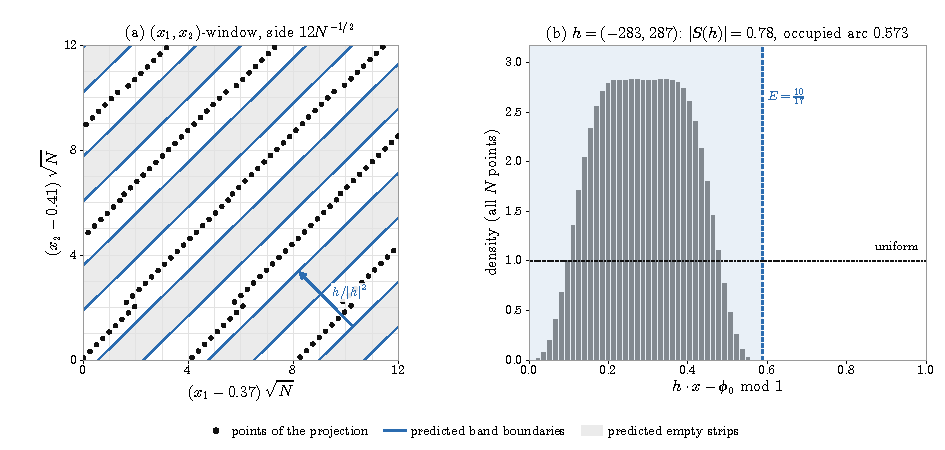
\includegraphics[width=\linewidth,height=0.45\textheight,keepaspectratio]{figs/projlines.pdf}}{\fbox{\parbox{0.9\textwidth}{\centering figure \texttt{projlines} pending}}}
\caption{\projLinesCaption}
\label{fig:projlines}
\end{figure}


\subsection{Reachable designs}
\begin{proposition}[Reachable designs]\label{prop:F}
The off-diagonal part of a design is reachable from the frame by the gauge moves of Lemma~\ref{lem:box}(c) with row scalars $\lambda'$ (that is, the residual problem is solvable with these $\lambda'$) if and only if, for every column $d$ and every $j\le s-2$,
\[
M^{(j)}[c][d]=\lambda'_c\,w_{cd}\,g_{d,j}(y_{cd})\qquad(c\ne d)
\]
for a polynomial $g_{d,j}\in R[X]$ of degree $j$ whose leading coefficient is a unit. For finite $c,d$ this says $M^{(j)}[c][d]=\lambda'_c\tilde g_{d,j}(z_{cd})$ with $z_{cd}=1/(a_c-a_d)$ and $\tilde g_{d,j}(z)=z\,g_{d,j}(z)$ of degree $j+1$ without constant term.
\end{proposition}

\begin{proof}
A lower-triangular column move with unit diagonal is a Toeplitz move times an upper-triangular matrix in the carry depths, so the residual problem captures all of Lemma~\ref{lem:box}(c) on row $0$. Column $n$ of $\lambda'^{-1}\odot F_{\cdot d}$ must be $\sum_{n'\le n}v_{n'}(U'_d)_{n'n}$, i.e. $(w_{cd}f_n(y_{cd}))_c$ with $\deg f_n\le n$ and the coefficient of $X^n$ a unit; as the $y_{cd}$ are distinct with unit differences, interpolation is unique over $R$, and this is exactly the condition. Partial sums of such polynomials have the same form, and conversely.
\end{proof}

At carry depth $0$ the design is the Cauchy layer $\lambda'_c\mu_dw_{cd}$; at carry depth $s-2$ any column whose interpolating polynomial has a unit leading coefficient is allowed (for instance a unit vector). Columns are coupled only through the shared row scalars $\lambda'_c$.

\subsection{Cauchy identities}
By Proposition~\ref{prop:Ns} the geometric layer stays a Cauchy matrix with free diagonal under the moves of Lemma~\ref{lem:box}(a), (c). In homogeneous coordinates $a_c=[\alpha_c:\beta_c]$, with $\infty=[1:0]$, put $D_{cd}=\alpha_c\beta_d-\alpha_d\beta_c$: then $D_{cd}=a_c-a_d$ for finite places, $D_{\infty d}=1$ and $D_{c\infty}=-1$, and the layer is $\tilde M_{cd}=\lambda_c\mu_d/D_{cd}$ ($c\ne d$) with units $\lambda_c$, $\mu_d$ (the sign of $D_{c\infty}$ is absorbed into $\mu_\infty$). The same holds over $\F_p$ for places in $\mathbb P^1(\F_p)$, and for the skeleton rows of Section~\ref{sec:skel} at carry depth $0$ (Proposition~\ref{prop:skelcomp}(i)). Put $\nu_c=\lambda_c\mu_c$ and $\pi_{cd}=\tilde M_{cd}\tilde M_{dc}=-\nu_c\nu_d/D_{cd}^2$.

\begin{lemma}[Cauchy identities]\label{lem:CH}
Let $R$ be a commutative ring, $\alpha,\beta\in R^s$, $D_{cd}=\alpha_c\beta_d-\alpha_d\beta_c$, and $W_{cd}=\lambda_c\mu_d/D_{cd}$ for $c\ne d$, where all $\lambda_c$, $\mu_d$ and $D_{cd}$ are units of $R$; let $\nu_c=\lambda_c\mu_c$ and $\pi_{cd}=W_{cd}W_{dc}$.
\begin{enumerate}
\item[(C)] For distinct $c,d,e$: $W_{cd}W_{de}W_{ec}=-W_{dc}W_{ed}W_{ce}$. Hence, if $R$ is an ordered field, $\pi_{cd}\pi_{de}\pi_{ec}<0$, and ``$c\sim d$ iff $\pi_{cd}<0$'' is an equivalence relation with at most two classes.
\item[(P)] For distinct $a,b,c,d$ let $\chi=D_{ac}D_{bd}/(D_{ab}D_{cd})$ and $\psi=D_{ad}D_{bc}/(D_{ab}D_{cd})$. Then $\chi-\psi=1$, $\chi^2=\pi_{ab}\pi_{cd}/(\pi_{ac}\pi_{bd})$ and $\psi^2=\pi_{ab}\pi_{cd}/(\pi_{ad}\pi_{bc})$; consequently $(\chi^2-\psi^2-1)^2=4\psi^2$.
\item[(H)] If $R\subset\R$: for distinct $i,j,k,l$, the largest of $|\pi_{ij}\pi_{kl}|^{-1/2}$, $|\pi_{ik}\pi_{jl}|^{-1/2}$, $|\pi_{il}\pi_{jk}|^{-1/2}$ is the sum of the other two.
\item[(X)] For distinct $i,j,l,d$:
\[
\frac{W_{ji}W_{ld}}{W_{jd}W_{li}}+\frac{W_{ij}W_{ld}}{W_{id}W_{lj}}=1 .
\]
\end{enumerate}
\end{lemma}

\begin{proof}
Everything follows from $D_{dc}=-D_{cd}$ and the Pl\"ucker relation $D_{ab}D_{cd}-D_{ac}D_{bd}+D_{ad}D_{bc}=0$. (C) The $\lambda$, $\mu$ cancel, and the $D$ cancel up to $(-1)^3$; then $\pi_{cd}\pi_{de}\pi_{ec}=-(W_{dc}W_{ed}W_{ce})^2$. If $c\sim d$ and $d\sim e$, two of the three factors are negative, so the third is too; if $c\not\sim d$ and $d\not\sim e$, then $c\sim e$. (P) Dividing the Pl\"ucker relation by $D_{ab}D_{cd}$ gives $\chi-\psi=1$. Since $\pi_{xy}=-\nu_x\nu_y/D_{xy}^2$, we have $\pi_{ab}\pi_{cd}=\nu_a\nu_b\nu_c\nu_d/(D_{ab}D_{cd})^2$ and similarly for the other pairings, which gives $\chi^2$ and $\psi^2$; and $\chi=1+\psi$ gives $2\psi=\chi^2-\psi^2-1$. (H) By the same formula $|D_{ij}D_{kl}|$, $|D_{ik}D_{jl}|$, $|D_{il}D_{jk}|$ are proportional to the three numbers, and by the Pl\"ucker relation the products sum to zero with signs. (X) The $\lambda$ and $\mu$ cancel, the two terms are $D_{jd}D_{il}/(D_{ij}D_{ld})$ and $-D_{id}D_{jl}/(D_{ij}D_{ld})$, and $D_{il}D_{jd}-D_{id}D_{jl}=D_{ij}D_{ld}$ is the Pl\"ucker relation for $(i,j,l,d)$.
\end{proof}

Each regime meets one of these identities as its frame-orbit obstruction: (X), or (P), modulo $q$ excludes $\pm1$ layers in dimension four (Remark~\ref{rem:pm1}); (C) and (H) exclude the deficit $K=1$ in dimension $s\ge5$ for the designs of Theorem~\ref{thm:O5}; (X) rules out, for $\ell\ge3$ skeleton coordinates (Section~\ref{sec:skel}), the Korobov skeleton digits that the nets $\mathcal B^1$ of Section~\ref{sec:allm} use in dimension three, when the faults are small (Lemma~\ref{lem:frameid}, Corollary~\ref{cor:frameid}); and (P), read $2$-adically, excludes half-integer layers (Proposition~\ref{prop:P}). The identities need the row and the column of a layer entry to carry the \emph{same} places; there are three ways out. The block scalings of Lemma~\ref{lem:box}(b), only for $s=3$, break the Cauchy form (the nets $\mathcal B^1$ of Definition~\ref{def:B} use them); graph forms at $m=s$ that are written down directly, not obtained from a frame, are not subject to it (Section~\ref{sec:large}); on split frames the layer $\lambda_c\mu_d/(u_c-v_d)$ has different row and column points and satisfies no Pl\"ucker relation (Proposition~\ref{prop:Gsplit}).

\section{Cubic cells, \texorpdfstring{$m\equiv0\pmod s$}{m = 0 mod s}: designs from short lattice vectors}\label{sec:dims}\label{sec:small}
At the resolutions $m=sk$ the cells are cubes. A geometric layer $\tilde M$ with bounded centred entries puts the points locally on $(I+\tilde M/q)\Z^s$, a slightly rotated and contracted $\Z^s$ broken along slip planes, at separation $1-K/q+O(q^{-2})$ (Remark~\ref{rem:K}). This section proves Theorem~A: a lower bound by diagonal dominance (Proposition~\ref{prop:D}) reduces the separation to the size of the entries of a reachable design, and the reachable design columns form a lattice whose short vectors make the entries small (Sections~\ref{sec:lattice} and~\ref{sec:Ustar}). Dimension three, where one integer scramble works in every base, follows in Section~\ref{sec:dim3}.

\subsection{Diagonal dominance}
We keep the notation of Section~\ref{sec:frames} and use the relaxation $\mathrm{LB}$ of Lemma~\ref{lem:Ss} with $L=\min(k,s-1)$ levels; for $k<s-1$ the frame realizes the truncated design $(F_0,\dots,F_{k-1})$ (Proposition~\ref{prop:Gs}).

\label{sec:U}
\begin{proposition}[Diagonal dominance]\label{prop:D}
Let $F$ be a reachable design whose diagonal vanishes at every carry depth $n\ge1$, with $F_0[c][c]=-\alpha_c$ and
\[
\alpha_c\ \ge\ \sum_{d\ne c}\ \max_{0\le j\le s-2}\bigl|M^{(j)}[c][d]\bigr|,\qquad a=\max_c\alpha_c.
\]
Then $\mathrm{LB}\ge1-a/q$ for every $q\ge5a+4$ (and every $k\ge1$).
\end{proposition}

\begin{proof}
Since the diagonal vanishes at every carry depth $n\ge1$, the own term of every moving coordinate $i$ is $-\alpha_i$ for every carry depth $j_i$, and dominance gives $e_i\sigma_i\le-\alpha_i+\alpha_i=0$ and $|\sigma_i|\le2a<q$: every moving coordinate is backward, so $b_i\ge q-|\sigma_i|-\mathrm{jit}_i$. An own-axis step along $c$ has $b_c=q-\alpha_c\ge q-a$ (no jitter). A step with at least two moving axes has $\sum b_i^2\ge2(q-2a-1)^2$, and $\sqrt2(q-2a-1)\ge q-a$ holds for $q\ge(2\sqrt2-1)a/(\sqrt2-1)+\sqrt2/(\sqrt2-1)$, in particular for $q\ge5a+4$. A truncated design is dominant with the same $a$, and at $k=1$ the configurations are a subset of those for $k\ge2$ (after Lemma~\ref{lem:Ss}).
\end{proof}

So the base threshold is $5a+4$, where $a$ measures the largest entries of the partial sums of a reachable design. By Proposition~\ref{prop:F} a design is reachable with row scalars $\lambda'$ if and only if each column of its partial sums interpolates a polynomial with a unit leading coefficient at the nodes $y_{cd}$; the question is how small such columns can be. The answer is a lattice problem.

\subsection{Admissible design columns form a lattice}\label{sec:lattice}
Fix $s\ge3$, the places $\infty,0,1,\dots,\nu$ with $\nu=s-2$, and the row scalars $\lambda'\equiv1$. Let $S$ be the set of primes $p\le \nu$ and $R_S=\Z[1/\nu!]$, so that the units of $R_S$ are $\pm$ the products of powers of primes in $S$ (the \emph{$S$-units}); for these places the ring $R$ of Section~\ref{sec:frames} is $R_S$. Fix a column $d$. For the $s-1$ rows $c\ne d$ let $w_c=w_{cd}$ and $y_c=y_{cd}$ be as in Proposition~\ref{prop:Ns}: $w_c=y_c=1/(c-d)$ if $c$ and $d$ are finite, $w_c=1$, $y_c=0$ for $c=\infty$, and $w_c=1$, $y_c=c$ for $d=\infty$. The weights $w_c$ and the differences $y_c-y_{c'}$, $c\ne c'$, are $S$-units: they are $1/(c-d)$, $(c'-c)/((c-d)(c'-d))$ or $c-c'$, with integers of absolute value at most $\nu$. For $0\le j\le \nu$ put
\[
V_j=\bigl\{(w_c\,g(y_c))_{c\ne d}:g\in\mathbb Q[X],\ \deg g\le j\bigr\}\subset\mathbb Q^{s-1},\qquad \Lambda_j=V_j\cap\Z^{s-1},
\]
and let $\operatorname{lc}_j:V_j\to\mathbb Q$ map a vector to the coefficient of $X^j$ in its polynomial $g$. As the $s-1$ nodes are distinct and $j\le s-2$, $g$ is determined by the vector, $\dim V_j=j+1$, $V_{j-1}\subset V_j$ is the kernel of $\operatorname{lc}_j$ ($V_{-1}=0$), and $V_\nu=\mathbb Q^{s-1}$. By Proposition~\ref{prop:F} (with $\lambda'\equiv1$, over $R_S$) an integer column $(M^{(j)}[c][d])_{c\ne d}$ is an \emph{admissible} design column at carry depth $j$ if it is a vector of $V_j$ whose polynomial has coefficients in $R_S$ and degree $j$ with an $S$-unit leading coefficient.

\begin{lemma}[The lattice of admissible design columns]\label{lem:sat}
\begin{enumerate}
\item[(i)] For $E\in\Lambda_j$ the polynomial of $E$ has coefficients in $R_S$.
\item[(ii)] $\operatorname{lc}_j(\Lambda_j)=\gamma_j\Z$ for a positive $S$-unit $\gamma_j$.
\item[(iii)] An integer column is admissible at carry depth $j$ if and only if it lies in $\Lambda_j$ and $\operatorname{lc}_j(E)$ is an $S$-unit; in particular every $E\in\Lambda_j$ with $\operatorname{lc}_j(E)=\gamma_j$ is admissible.
\item[(iv)] If $E_i\in\Lambda_i$ and $\operatorname{lc}_i(E_i)=\gamma_i$ for $i=0,\dots,j$, then $E_0,\dots,E_j$ is a basis of $\Lambda_j$, and $\{E\in\Lambda_j:\operatorname{lc}_j(E)=\gamma_j\}=E_j+\Lambda_{j-1}$.
\end{enumerate}
\end{lemma}

\begin{proof}
(i) Lagrange interpolation at any $j+1$ rows $J$ recovers $g=\sum_{b\in J}(E_b/w_b)\prod_{b'\in J\setminus b}(X-y_{b'})/(y_b-y_{b'})$, and all denominators are $S$-units. (ii) $\operatorname{lc}_j(\Lambda_j)$ is a finitely generated subgroup of $\mathbb Q$, nonzero because $\Lambda_j$ spans $V_j$, so it is $\gamma_j\Z$ with $\gamma_j>0$; by (i), $\gamma_j\in R_S$. The vector $(w_cy_c^j)_c$ of $g=X^j$ has $S$-unit or zero entries, so some product $P$ of primes in $S$ makes $P(w_cy_c^j)_c$ integral, with $\operatorname{lc}_j=P$; hence $P\in\gamma_j\Z$, and $\gamma_j$ has no prime factor outside $S$ in its numerator either. (iii) is (i) together with the definition. (iv) If $v\in\Lambda_j$ has $\operatorname{lc}_j(v)=t\gamma_j$, then $v-tE_j\in\Lambda_j\cap\ker\operatorname{lc}_j=\Lambda_{j-1}$; induction on $j$.
\end{proof}

So the admissible design columns at carry depth $j$ are the lattice vectors on the affine hyperplanes $\operatorname{lc}_j=\pm\gamma_j\cdot(S\text{-unit})$ of $\Lambda_j$, and the smallest ones are governed by the distance between consecutive hyperplanes. That distance is a product of local Chebyshev constants, one for each place of $\mathbb Q$ that matters (in the sense of number theory: the archimedean absolute value and the $p$-adic ones; not the places of a frame). For the archimedean absolute value and each $p\in S$ let
\[
A_{j,\R}=\min\bigl\{\|E\|_2:E\in V_j\otimes\R,\ \operatorname{lc}_j(E)=1\bigr\},\qquad A_{j,p}=\min\bigl\{\max_c|E_c|_p:E\in V_j,\ \operatorname{lc}_j(E)=1\bigr\},
\]
the least size, at that place, of the vectors $(w_cg(y_c))_c$ of monic polynomials $g$ of degree $j$ (the minimum at $p$ exists because these sizes are powers of $p$ and are bounded below by Lagrange interpolation).

\begin{lemma}[Adelic Chebyshev identity]\label{lem:adelic}
Let $\pi_j$ be the orthogonal projection of $\R^{s-1}$ onto the line $V_j\cap V_{j-1}^\perp$. Then $\pi_j(\Lambda_j)$ is generated by a vector of length
\[
\eta_j=A_{j,\R}\prod_{p\in S}A_{j,p},\qquad\text{and}\qquad \gamma_j=\prod_{p\in S}A_{j,p}.
\]
Every $E\in\Lambda_j\setminus V_{j-1}$ has $\|E\|_2\ge \eta_j$.
\end{lemma}

\begin{proof}
\emph{The $p$-adic places, $p\in S$.} If $E\in V_j$ has $\operatorname{lc}_j(E)=1$ and $\max_c|E_c|_p=p^e$, then $p^eE$ is $p$-integral, and $D'p^eE\in\Lambda_j$ for an integer $D'$ prime to $p$; so $D'p^e\in\gamma_j\Z$ and $v_p(\gamma_j)\le e$. Conversely, for $v\in\Lambda_j$ with $\operatorname{lc}_j(v)=\gamma_j$ the vector $v/\gamma_j$ has $\operatorname{lc}_j=1$ and $\max_c|v_c/\gamma_j|_p\le p^{v_p(\gamma_j)}$. So $A_{j,p}=p^{v_p(\gamma_j)}$, and as $\gamma_j>0$ is an $S$-unit, $\gamma_j=\prod_{p\in S}A_{j,p}$. \emph{The archimedean place.} On $V_j$, $\operatorname{lc}_j(E)=\langle\theta,E\rangle$ for a unique $\theta\in V_j$, and $\theta\perp V_{j-1}$. Hence $\|\pi_j(E)\|=|\operatorname{lc}_j(E)|/\|\theta\|$, and the least norm with $\operatorname{lc}_j=1$ is $A_{j,\R}=1/\|\theta\|$, attained at $\theta/\|\theta\|^2$. So $\pi_j(\Lambda_j)=\gamma_j\Z\,\theta/\|\theta\|^2$, generated by a vector of length $\gamma_jA_{j,\R}=\eta_j$, and $\|E\|\ge\|\pi_j(E)\|\ge \eta_j$ if $\operatorname{lc}_j(E)\ne0$.
\end{proof}

This is the product formula at work: an $S$-unit scalar can move the $p$-adic cost of a collision of nodes (Proposition~\ref{prop:Ns}) to the archimedean place, but never remove it. For the upper bounds below it suffices to exhibit, \emph{independently at each place}, one monic polynomial that is small there. At the place $p$ a monic polynomial is small on the nodes if its roots sit $p$-adically near the nodes that collide modulo $p$ (two finite rows $c,c'$ collide if $p\mid c-c'$, and then $y_c$ is $p$-adically large); different primes want the roots in different places, so no single closed-form basis serves all primes, and the lattice reduction chooses the roots for each prime automatically.

\begin{lemma}[Babai rounding along the flag]\label{lem:babai}
Let $E_i\in\Lambda_i$ with $\operatorname{lc}_i(E_i)=\gamma_i$ for $i<j$, and let $v\in\Lambda_j$ with $\operatorname{lc}_j(v)=\gamma_j$. Write the orthogonal projection of $v$ onto $V_{j-1}$ as $\sum_{i<j}c_iE_i$ and put $E_j=v-\sum_{i<j}\lfloor c_i+\frac12\rfloor E_i$. Then $E_j\in\Lambda_j$, $\operatorname{lc}_j(E_j)=\gamma_j$, and
\[
\|E_j\|_2\le \eta_j+\tfrac12\textstyle\sum_{i<j}\|E_i\|_2 .
\]
Consequently, if $E_0,\dots,E_j$ are all obtained in this way and $\eta_i\le H$ for every $i\le j$, then $\|E_i\|_2\le(3/2)^iH$ for every $i\le j$.
\end{lemma}

\begin{proof}
$E_j-v\in\Lambda_{j-1}=\ker\operatorname{lc}_j\cap\Lambda_j$, and $E_j=\pi_j(v)+\sum_{i<j}\bigl(c_i-\lfloor c_i+\frac12\rfloor\bigr)E_i$ with $\|\pi_j(v)\|=\eta_j$ (Lemma~\ref{lem:adelic}) and every coefficient in $[-\frac12,\frac12]$. For the consequence let $T_i=\sum_{i'\le i}\|E_{i'}\|$. Then $T_0=\eta_0\le H$ and $T_i\le\frac32T_{i-1}+H$, so $T_i\le2H((3/2)^{i+1}-1)$ by induction, and $\|E_i\|\le H+\frac12T_{i-1}\le(3/2)^iH$.
\end{proof}

\subsection{The design \texorpdfstring{$U^*_s$}{U*s} and the proof of Theorem~A}\label{sec:Ustar}
\begin{definition}[The design $U^*_s$]\label{def:Ustar}
Let $s\ge3$, $\nu=s-2$, and take the places $\infty,0,1,\dots,\nu$ and $\lambda'\equiv1$. For each column $d$ let $E_{d,0}$ be the generator of $\Lambda_0$ with $\operatorname{lc}_0>0$, and for $1\le j\le \nu$ let $E_{d,j}$ be the unique $E\in\Lambda_j$ with $\operatorname{lc}_j(E)=+\gamma_j$ whose orthogonal projection onto $V_{j-1}$ has all its coefficients in the basis $E_{d,0},\dots,E_{d,j-1}$ in $[-\frac12,\frac12)$. The design $U^*_s=(F_0,\dots,F_\nu)$ has the partial sums $M^{(j)}[c][d]=E_{d,j}[c]$ ($c\ne d$, $j\le \nu$), the diagonal $F_0[c][c]=-\alpha_c$ at carry depth $0$ with $\alpha_c=\sum_{d\ne c}\max_j|E_{d,j}[c]|$, and zero diagonal at the carry depths $n\ge1$. Let $a^*_s=\max_c\alpha_c$.
\end{definition}

By Lemma~\ref{lem:sat}(iv) the set $\{E\in\Lambda_j:\operatorname{lc}_j(E)=\gamma_j\}$ is a coset of $\Lambda_{j-1}=\bigoplus_{i<j}\Z E_{d,i}$, so $E_{d,j}$ exists, is unique, and is the vector of Lemma~\ref{lem:babai} for any $v$ in that coset (with ties rounded up). Only the two conventions $\operatorname{lc}_j=+\gamma_j$ and ``ties up'' matter: the result does not depend on the choice of $v$, of a basis of $\Lambda_j$ or of the order of the rows. The construction is deterministic and runs in time polynomial in $s$: there are $s(s-1)$ pairs $(d,j)$, each needs an integer kernel and a Hermite normal form of a lattice of dimension at most $s-1$ with entries of $O(s^2\log s)$ bits \cite{KB79}, an extended Euclid step for $v$, and one rational Gram solve, and the output entries have $O(s\log s)$ bits by the proof below; it is not a closed formula. For $s=3$ (places $\infty,0,1$, $S=\emptyset$) the definition gives, in the coordinate order $\infty,0,1$,
\[
F_0=\begin{pmatrix}-2&1&1\\1&-2&-1\\1&1&-2\end{pmatrix},\qquad F_1=\begin{pmatrix}0&-2&-1\\-2&0&2\\-1&-1&0\end{pmatrix},
\]
so $a^*_3=2$. Table~\ref{tab:astar} lists $a^*_s$ for $s\le10$ (computed exactly by two independent implementations of Definition~\ref{def:Ustar}).

\begin{table}[tbp]
\centering\small\setlength{\tabcolsep}{4pt}
\begin{tabular}{@{}lcccccccc@{}}
\toprule
$s$ & 3 & 4 & 5 & 6 & 7 & 8 & 9 & 10\\
\midrule
$a^*_s$ & 2 & 5 & 16 & 43 & 170 & 543 & 2842 & 13640\\
largest entry of $U^*_s$ & 1 & 2 & 6 & 14 & 86 & 198 & 1446 & 5364\\
$5a^*_s+4$ & 14 & 29 & 84 & 219 & 854 & 2719 & 14214 & 68204\\
bound of Theorem~A & -- & 46.7 & 324 & 2716 & $2.67\cdot10^4$ & $3.03\cdot10^5$ & $3.89\cdot10^6$ & $5.58\cdot10^7$\\
$a_s$ of $U_s$ (Remark~\ref{rem:Us}) & 4 & 63 & 17407 & $5.67\cdot10^6$ & $1.86\cdot10^{12}$ & $2.05\cdot10^{14}$ & $1.34\cdot10^{23}$ & $5.57\cdot10^{28}$\\
\bottomrule
\end{tabular}
\medskip
\caption{The constant $a^*_s$ of Theorem~\ref{thm:A} (exact values of Definition~\ref{def:Ustar}, computed), the largest entry $\max|M^{(j)}|$ of $U^*_s$, the base threshold $5a^*_s+4$, the bound $2(s-1)^{3/2}(3/2)^{s-2}(s-2)!$ of Theorem~A (truncated), and, for comparison, the constant $a_s$ of the monomial design $U_s$.}
\label{tab:astar}
\end{table}

\begin{proof}[Proof of Theorem~\ref{thm:A}]
\emph{Reachability.} By Lemma~\ref{lem:sat}(iii) every column $E_{d,j}$ is admissible at carry depth $j$, with polynomial $g_{d,j}\in R_S[X]$ of degree $j$ and leading coefficient $\gamma_j$, an $S$-unit; so by Proposition~\ref{prop:F} the off-diagonal part of $U^*_s$ is reachable with $\lambda'\equiv1$ over $R'=R_S$, and the diagonal is free (Lemma~\ref{lem:box}(a)).

(1) Every prime factor of $q$ is at least $s-1>\nu$, so $\gcd(q,\nu!)=1$, and Corollary~\ref{cor:tsk} gives a digital $(0,sk,s)$-net with one point in every cell, for every $k\ge1$. A cell has diameter $\sqrt s\,q^{-k}=\sqrt s\,N^{-1/s}$, which bounds $h$.

(2) \emph{Lower bound.} (H1) and (H2) of Lemma~\ref{lem:Ss} hold by Proposition~\ref{prop:Gs} and Definition~\ref{def:Ns}, with $L=\min(k,s-1)$. $U^*_s$ is diagonally dominant by construction, with the maximum over all carry depths, so Proposition~\ref{prop:D} gives $\delta q^k\ge1-a^*_s/q$ for $q\ge5a^*_s+4$ and every $k\ge1$.

\emph{Sharpness} ($k\ge2$). Let $i$ attain $a^*_s=\alpha_i$. For $q>2a^*_s$ the entries of $F_0$ are centred, so $\tilde M=F_0$. By (H2) the own-axis step $e_i$ from a cell whose last digit of $n_i$ is not $q-1$ changes coordinate $i$ by exactly $1-a^*_s/q$ cells if its first offset digit is at least $a^*_s$ (no wrap, no jitter), and every other coordinate $u$ by less than $(|\tilde M_{ui}|+1)/q$ if $r_u$ avoids the $|\tilde M_{ui}|$ values from which adding $\tilde M_{ui}$ wraps. For each $u\ne i$ the $t=0$ box with depths $k+1$ on $i$ and $u$ and $0$ elsewhere (total $2k+2\le sk$) makes $(n_i,r_i,n_u,r_u)$ jointly uniform (that box fixes exactly these $2k+2$ digits, so every value of them occurs equally often), so among the cells satisfying the conditions on $n_i$ and $r_i$ the fraction with a wrapping $r_u$ is $|\tilde M_{ui}|/q$; for $q>\sum_{u\ne i}|\tilde M_{ui}|$ a union bound leaves a cell. Its pair of points lies inside the unit cube, so
\[
\delta N^{1/s}<\Bigl(\bigl(1-\tfrac{a^*_s}q\bigr)^2+\sum_{u\ne i}\frac{(|F_0[u][i]|+1)^2}{q^2}\Bigr)^{1/2}=1-\frac{a^*_s}q+O(q^{-2}).
\]

\emph{The bound on $a^*_s$.} Let $s\ge4$. By Lemma~\ref{lem:babai} it suffices to show $\eta_{d,j}\le \Xi_s:=2\sqrt{s-1}\,(s-2)!$ for every column $d$ and carry depth $j$; then every entry of $U^*_s$ is at most $\max_{d,j}\|E_{d,j}\|_2\le(3/2)^{s-2}\Xi_s$, and $a^*_s\le(s-1)(3/2)^{s-2}\Xi_s=2(s-1)^{3/2}(3/2)^{s-2}(s-2)!$. By Lemma~\ref{lem:adelic} it suffices to give, at each place of $\mathbb Q$, one monic $g$ of degree $j$.

\emph{Finite column $d$.} Archimedean place: all nodes $y_c$ lie in $[-1,1]$ and $|w_c|\le1$, so the monic Chebyshev polynomial $2^{1-j}T_j$ ($j\ge1$; $g=1$ for $j=0$) gives $A_{j,\R}\le2\sqrt{s-1}$. At $p\in S$: let $\mathcal R_p$ be the finite rows $c\ne d$ with $p\mid c-d$, $e_c=v_p(c-d)\ge1$ for $c\in \mathcal R_p$, let $\mathcal R'\subset \mathcal R_p$ consist of $\min(j,|\mathcal R_p|)$ rows with the largest $e_c$, and $g_p=\prod_{r\in \mathcal R'}(X-y_r)\cdot X^{j-|\mathcal R'|}$. For $c\in \mathcal R'$ the entry vanishes. For $c,r\in \mathcal R_p$, $|y_c-y_r|_p=|(r-c)/((c-d)(r-d))|_p\le p^{\max(e_c,e_r)}$; so for $c\in \mathcal R_p\setminus \mathcal R'$ (then $|\mathcal R'|=j$ and $e_c\le e_r$ for $r\in \mathcal R'$) the entry has $p$-adic size at most $p^{e_c+\sum_{r\in \mathcal R'}e_r}\le p^{\sum_{r\in \mathcal R_p}e_r}$. For a finite row $c\notin \mathcal R_p$, and for the row $\infty$ ($y=0$, $w=1$), $|w_c|_p=1$, $|y_c|_p\le1$ and $|y_c-y_r|_p\le p^{e_r}$, so the size is at most $p^{\sum_{r\in \mathcal R'}e_r}$. Hence $A_{j,p}\le p^{\sum_{r\in \mathcal R_p}e_r}=p^{v_p(d!\,(\nu-d)!)}$, and $\prod_{p\in S}A_{j,p}\le d!\,(\nu-d)!\le \nu!$, since every prime factor of $d!(\nu-d)!$ lies in $S$. So $\eta_{d,j}\le2\sqrt{s-1}\,\nu!$.

\emph{Column $\infty$.} The nodes are $y_c=c\in\{0,\dots,\nu\}$ with $w_c=1$. At the archimedean place the monic Chebyshev polynomial of $[0,\nu]$ gives $A_{j,\R}\le2\sqrt{s-1}\,(\nu/4)^j$. At $p\in S$ the falling factorial $X(X-1)\cdots(X-j+1)$ takes the values $j!\binom cj$, so $A_{j,p}\le|j!|_p$ and $\prod_pA_{j,p}\le1/j!$. So $\eta_{\infty,j}\le2\sqrt{s-1}\,(\nu/4)^j/j!\le2\sqrt{s-1}\,e^{\nu/4}\le2\sqrt{s-1}\,\nu!$ for $\nu\ge2$.

Finally, with $\nu=s-2$ the elementary bounds $\nu^\nu e^{-\nu}\le \nu!\le \nu^\nu$ give $\bigl|\log\bigl(2(s-1)^{3/2}(3/2)^{s-2}(s-2)!\bigr)-s\log s\bigr|\le3s$ for $s\ge4$, so the bound is $e^{s\log s+O(s)}$; and $a^*_3=2$ is the display before Table~\ref{tab:astar}. (At the archimedean place the Chebyshev polynomial even gives $A_{j,\R}\le\sqrt{s-1}$ for a finite column, since $|2^{1-j}T_j|\le1$ on $[-1,1]$ for $j\ge1$; the factor $2$ in $\Xi_s$ is slack.)
\end{proof}

The bound is far from the computed values: $5.58\cdot10^7$ against $a^*_{10}=13640$ (Table~\ref{tab:astar}). The proof shows where the size comes from: the archimedean Chebyshev constants are harmless, and the cost sits at the primes $p\le s-2$, through the factorials $d!(s-2-d)!$ of the place differences. Whether other row scalars $\lambda'$, other places or another lower-bound argument bring the base threshold down to a polynomial in $s$ is open.

\begin{figure}[tbp]
\centering
\IfFileExists{figs/thmA_design.pdf}{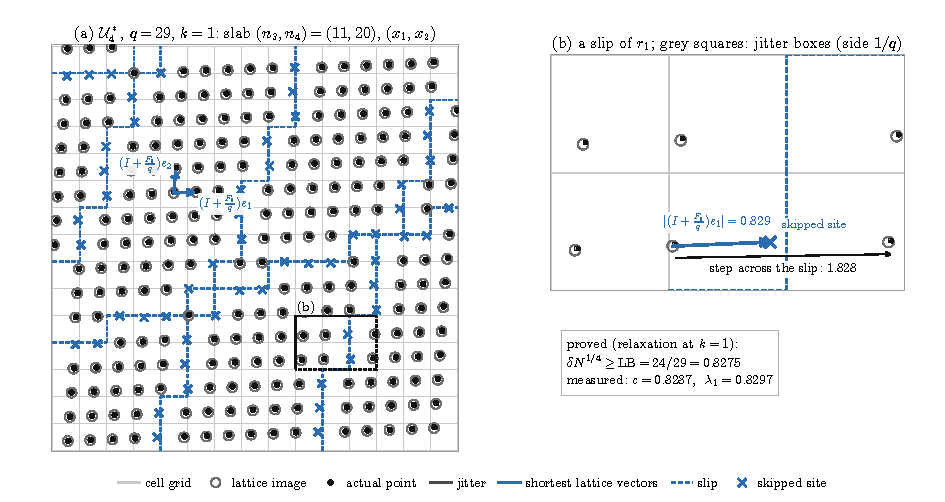
\includegraphics[width=\linewidth,height=0.62\textheight,keepaspectratio]{figs/thmA_design.pdf}}{\fbox{\parbox{0.9\textwidth}{\centering figure \texttt{thmA\_design} pending}}}
\caption{\thmADesignCaption}
\label{fig:thmA}
\end{figure}

\begin{remark}[The monomial design $U_s$]\label{rem:Us}
The every-dimension theorem also holds with the monomial design $U_s$: put $L_s=\operatorname{lcm}(1,\dots,s-2)^{s-1}$, $\lambda'_c=L_s$ for finite $c$, $\lambda'_\infty=1$, and $F_n[c][d]=L_s/(c-d)^{n+1}$ for finite $c,d$, $F_n[\infty][d]=[n=0]$, $F_n[c][\infty]=L_s\binom cn$, with a diagonal that is dominant in the sense of Proposition~\ref{prop:D}. Its increments are monomials in the nodes, and the proof of Theorem~A applies verbatim with its constant $a_s=\max_c\alpha_c$ in place of $a^*_s$ (for $k\ge2$ the net property, the separation bound for $q\ge5a_s+4$ and the sharpness are formally verified for this design). But $\log a_s=(1+o(1))s^2$: for finite $c$, $\alpha_c\ge|F_0[c][\infty]|=L_s$, and $\log L_s=(s-1)\psi(s-2)$ with Chebyshev's function $\psi$, while $a_s\le L_s(s^2+2^{s-2})$; so $a_s=e^{\Theta(s^2)}$ already by Chebyshev's bounds $\psi(x)\asymp x$, and the constant $1$ uses the prime number theorem \cite{Had96,dlVP96}. In the language above the reason is $p$-adic: a monomial has all its roots at $0$, so at a collision of nodes it is as large as possible, $|y^j|_p=p^{j\,v_p(c-d)}$, at every carry depth and in every column, and the single row scalar $\lambda'$ must clear all of it. Theorem~A puts the roots near the colliding nodes, separately for each prime, and so replaces $e^{\Theta(s^2)}$ by the upper bound $e^{s\log s+O(s)}$ (Table~\ref{tab:astar}: $a_5=17407$ against $a^*_5=16$).
\end{remark}

\section{Lattice skeletons: \texorpdfstring{$m=sk+r$}{m=sk+r}}\label{sec:skel}
For $N=p^m$, $m=sk+r$ with $1\le r\le s-1$, the boxes with one point each cannot all be cubes (regime~II of Section~\ref{sec:prelim}, Figure~\ref{fig:arcskeleton}). We give $r$ coordinates $k+1$ cell digits (the \emph{full} coordinates) and the other $\ell=s-r$ coordinates only $k$ (the \emph{skeleton} coordinates). The first offset digit of a skeleton coordinate, its \emph{skeleton digit}, places the point, along that coordinate, in one of the $p$ sub-intervals of side $p^{-(k+1)}$ of its cell. So we measure positions in \emph{fine cells}, the cubes of side $p^{-(k+1)}$: a cell (with the depths above) consists of $p^\ell$ fine cells, and each point lies in one of them. A \emph{coarse block} is a cube of side $p^{-k}$, fixed by the first $k$ digits of every coordinate; it consists of $p^s$ fine cells and holds $p^r$ points. The skeleton digits build the lattice (the `skeleton') on which the occupied fine cells lie: inside each coarse block they form a coset of a lattice of index $p^\ell$, a Construction~A lattice of an MDS code (Remark~\ref{rem:codes}). From one block to the next this coset is shifted by a small vector, a \emph{fault}; the faults come from the coefficients $g_{ij}$ of Lemma~\ref{lem:skelnec}(N2). So the separation, in fine cells, is at least the lattice minimum minus the largest fault minus one fine cell for the deeper digits (Lemma~\ref{lem:skelred}). One skeleton coordinate needs no faults (Theorem~\ref{thm:S1}); two force them (Theorems~\ref{thm:S2} and~\ref{thm:allm}). For three or more, a Pl\"ucker identity satisfied by every net in the frame orbit (Section~\ref{sec:frames}) rules out the Korobov skeleton digits of the nets $\mathcal B^1$ when the faults are small (Corollary~\ref{cor:frameid}); these residues are open for all large primes.

\emph{Conventions.} Here $p$ is a prime, $s\ge3$ and $\ell=s-r$. The $r$ \emph{full} coordinates $x_1,\dots,x_r$ have depth $k+1$, the $\ell$ skeleton coordinates $z_1,\dots,z_\ell$ depth $k$, and $S_z$ denotes the skeleton digit of $z$. Level $l$ of the cells is $x_{d,l}$, $z_{j,l}$ (level $0$ is the most significant; the letter $x$ has nothing to do with the variable $x$ of Lemma~\ref{lem:Rs}). As in Section~\ref{sec:prelim}, the depth of a coordinate is its number of cell digits, and the last level of a coordinate of depth $k_c$ is at carry depth $0$, the level $k_c-1-n$ at carry depth $n$. In dimension three ($m=3k+r$) the coordinates are $(x,y,z)$, with depths $\mathbf k=(k+1,k,k)$ for $r=1$ ($\ell=2$) and $\mathbf k=(k+1,k+1,k)$ for $r=2$ ($\ell=1$), and cell levels $x_l$, $y_l$, $z_l$.

\subsection{Fine cells and the separation reduction}\label{sec:fine}
Fine cells have side $p^{-(k+1)}$ in every coordinate, and the fine unit is $\varpi=p^{m-k-1}$ integer units. Put $P_c=n_c$ for a full and $P_c=p\,n_c+S_c$ for a skeleton coordinate, where $n_c$ is the cell index as an integer. So $P_c$ is the position of the point along axis $c$ measured in fine cells: for a full coordinate its $k+1$ cell digits, for a skeleton coordinate its $k$ cell digits followed by the skeleton digit. Then $P_c\in[0,p^{k+1})$ is the \emph{fine cell} of coordinate $c$, and the integer coordinate is $X_c=P_c\varpi+\theta_c$ with $0\le\theta_c<\varpi$. Since $n_c=\lfloor P_c/p\rfloor$ for skeleton coordinates, $P$ determines all cell digits, hence the index: distinct points have distinct $P$. For a full coordinate, level $k-j$ is $\lfloor P_c/p^j\rfloor\bmod p$; for a skeleton coordinate, level $k-1-j$ is $\lfloor P_c/p^{j+1}\rfloor\bmod p$, and $P_c\equiv S_c\pmod p$.

\begin{lemma}[Separation reduction]\label{lem:skelred}\label{lem:fine}
Let $v\ne w$ be two points, and let $a_c$ be the centred residue ($-p^{k+1}/2<a_c\le p^{k+1}/2$) of $P_c(w)-P_c(v)$ modulo $p^{k+1}$; we call $a$ the \emph{fine difference} of $v$ and $w$.
\begin{enumerate}
\item[(i)] The toroidal distance of $X_c(w)$ and $X_c(v)$ modulo $N$ is at least $(|a_c|-1)\varpi$. Hence, if $|a|_\infty\ge M$ for every pair of distinct points, the toroidal minimum distance satisfies $\delta N^{1/s}\ge(M-1)\,p^{-\ell/s}$.
\item[(ii)] If $|a_c|<p$ and $1\le j\le k$, then $\lfloor P_c(w)/p^j\rfloor-\lfloor P_c(v)/p^j\rfloor\equiv\xi_{c,j}\pmod{p^{k+1-j}}$ with $\xi_{c,j}\in\{0,\sgn a_c\}$, and $\xi_{c,j}\ne0$ implies $\xi_{c,j-1}\ne0$ for $j\ge2$.
\end{enumerate}
\end{lemma}

\begin{proof}
(i) $N=p^{k+1}\varpi$, so $X_c(w)-X_c(v)\equiv x:=a_c\varpi+(\theta'-\theta)\pmod N$ with $|\theta'-\theta|<\varpi$. If $|x|\le N/2$, the distance is $|x|\ge|a_c|\varpi-(\varpi-1)$. Otherwise it is $N-|x|\ge N-(|a_c|+1)\varpi+1>(p^{k+1}-|a_c|-1)\varpi\ge(|a_c|-1)\varpi$, as $|a_c|\le p^{k+1}/2$. So $\delta N\ge(M-1)\varpi$, and $\varpi N^{1/s}/N=p^{m/s-k-1}=p^{-\ell/s}$. (ii) Write $P_c(w)=P_c(v)+a_c+\varepsilon p^{k+1}$ with $\varepsilon\in\{-1,0,1\}$. The difference of the floors is $\lfloor(P_c(v)+a_c)/p^j\rfloor-\lfloor P_c(v)/p^j\rfloor+\varepsilon p^{k+1-j}$. As $|a_c|<p\le p^j$, the first part lies in $\{0,\sgn a_c\}$, and it is nonzero only if a multiple of $p^j$, hence of $p^{j-1}$, lies between $P_c(v)$ and $P_c(v)+a_c$. Neither part uses that $p$ is odd or prime; $p\ge2$ suffices.
\end{proof}

Part (ii) says: if two points are less than $p$ fine cells apart along axis $c$, the cell digits above the fine one change only by one carry or borrow in the direction of $a_c$, and a change at a level implies a change at every less significant level. So along each coordinate the changed levels are the last $j$ levels for some $j$, all changed with the same sign $\sgn a_c$ (a \emph{sign-consistent prefix}). Every lattice $\Lambda\subset\Z^s$ of index $p^\ell$ has a nonzero vector with $|\cdot|_\infty\le\lfloor p^{\ell/s}\rfloor$ (pigeonhole: the cube $\{0,\dots,\lfloor p^{\ell/s}\rfloor\}^s$ has more than $p^\ell$ points, so two of them are congruent modulo $\Lambda$). So when all fine differences lie in one lattice of index $p^\ell$, as for $\ell=1$ (Theorem~\ref{thm:S1}), the bound of (i) is less than $1$. For $\ell\ge2$ only differences within one coarse block are lattice vectors, so there this ceiling is a heuristic, not a theorem.

\subsection{Necessary conditions, forced faults and completion}
\begin{lemma}[Necessary conditions on the skeleton digits]\label{lem:skelnec}
Let a graph form with the depths above be a $(0,m,s)$-net over $\F_p$. Let $A\in\F_p^{\ell\times r}$ hold the coefficients of the skeleton digits on the last levels $x_{d,k}$, and, for $k\ge1$ and $i\ne j$, let $g_{ij}$ be the coefficient of $S_{z_i}$ on $z_{j,k-1}$.
\begin{enumerate}
\item[(N1)] Every square submatrix of $A$ is invertible.
\item[(N2)] \emph{(Forced faults.)} If $\ell\ge2$ and $k\ge1$, then $g_{ij}\ne0$ for all $i\ne j$.
\item[(N3)] For every full coordinate $x_d$ and every set $I$ of $j$ skeleton coordinates, the coefficients of the $S_{z_i}$, $i\in I$, on the levels $x_{d,k},\dots,x_{d,k-j+1}$ form an invertible matrix; for a skeleton coordinate $z_e\notin I$ the same holds on the levels $z_{e,k-1},\dots,z_{e,k-j}$ (whenever these levels exist).
\end{enumerate}
\end{lemma}

\begin{proof}
All three follow from Lemma~\ref{lem:box} for suitable boxes. For (N1) take depth $k+1$ on the skeleton coordinates of a set $I$, depth $k$ on the full coordinates of a set $J$ with $|J|=|I|$, and $k_c$ elsewhere: the over coordinates are those of $I$, by one digit (their skeleton digits), the under coordinates those of $J$, by one level (the level $k$), and the minor is $\det A[I,J]$. (N2) is the box with depth $k+1$ on $z_i$ and $k-1$ on $z_j$; (N3) the box with depth $k+1$ on $I$ and $k_e-j$ on the coordinate $e$.
\end{proof}

In words, (N3) says that any $j$ of the skeleton digits together depend invertibly on the last $j$ cell levels of each other coordinate. We call the coefficients $g_{ij}$ the \emph{faults}. By (N2), for $\ell\ge2$ every skeleton digit depends, with a nonzero coefficient, on the last cell digit of every other skeleton coordinate: when the last cell digit of $z_j$ changes, the skeleton digit of $z_i$ shifts by $g_{ij}$, and with it the lattice coset of the occupied fine cells. So the occupied fine cells form a lattice coset only inside each coarse block, shifted by the faults between neighbouring blocks (as for $\mathcal B^1$, Section~\ref{sec:allm}). In our constructions the faults are bounded integers (centred), so at the lattice scale $p^{\ell/s}$ they cost a bounded number of fine cells.

Fix $s$ distinct places in $\mathbb P^1(\F_p)$ (so $p\ge s-1$) and assign them to the coordinates. Lemmas~\ref{lem:Ts}, \ref{lem:Rs} and Proposition~\ref{prop:Ns} hold verbatim over $\F_p$, since their proofs use only that the differences of the finite places are units. By Lemma~\ref{lem:Ts} the frame has a graph form $\Phi^F$ with depths $\mathbf k$, all of whose box minors are units.

The key observation behind the next proposition: the points of the frame with $s(k+1)$ digits whose skeleton coordinates start with the digit $0$ form, after these coordinates are rescaled by $p$, the frame with $m$ digits, and a skeleton digit is the old first offset digit.

\begin{proposition}[Completion]\label{prop:skelcomp}
Let the frame and $\Phi^F$ be as above.
\begin{enumerate}
\item[(i)] \emph{(Normal form.)} After the moves of Proposition~\ref{prop:Ns}, applied to the restricted frame as described in the proof below, row $0$ of every block $(z_i,d)$, $d\ne z_i$, of $\Phi^F$ has the generating function $w_{id}/(1-y_{id}x)$ of Proposition~\ref{prop:Ns}, where $x^n$ marks carry depth $n$, the level $k_d-1-n$; this holds for every $k$. For a column block $d$ let $\ell_d$ be the number of skeleton coordinates other than $d$ ($\ell_d=\ell$ if $d$ is full, $\ell_d=\ell-1$ if $d$ is a skeleton coordinate). Then Propositions~\ref{prop:F} and~\ref{prop:Gs} hold for the skeleton rows, with the $\ell_d$ skeleton rows $z_i\ne d$ of block $d$ in place of the rows $c\ne d$, and $\ell_d-1$, $\ell_d$ in place of $s-2$, $s-1$ (the carry depths $n\le\ell_d-1$).
\item[(ii)] \emph{($\ell=1$.)} For every $k\ge0$ and all units $\kappa_1,\dots,\kappa_r$, the moves of Lemma~\ref{lem:box} turn $\Phi^F$ into a graph form whose skeleton digit is $S_z=\sum_d\kappa_dx_{d,k}$ (all other entries of row $0$ of $z$, own block included, are $0$). It is a $(0,m,s)$-net over $\F_p$.
\item[(iii)] \emph{($\ell=2$.)} Let $k\ge1$ and prescribe skeleton digits
\[
S_{z_i}=\sum_dA_{id}\,x_{d,k}+\sum_d\beta_{id}\,x_{d,k-1}+g_{ij}\,z_{j,k-1}+o_i\,z_{i,k-1}\qquad(\{i,j\}=\{1,2\})
\]
satisfying (N1)--(N3), with arbitrary own coefficients $o_i$. For a suitable choice of the places they are reachable for every $k\ge1$, and they complete to a $(0,m,s)$-net over $\F_p$.
\end{enumerate}
\end{proposition}

\begin{proof}
(i) \emph{Restriction.} Let $m'=s(k+1)$ and $V\in\F_p[t]_{<m'}$. The first digit of the reading at a finite skeleton place $a_z$ vanishes iff $(t-a_z)\mid V$, and at $\infty$ iff $\deg V<m'-1$. So the points of the $m'$-frame whose skeleton coordinates have first digit $0$ are given by $V=\prod_{z\text{ finite}}(t-a_z)\,V'$ with $\deg V'<m$, and their readings are those of $V'$ times a unit power series, shifted by one digit at a skeleton place. Hence this point set, with the skeleton coordinates rescaled by $p$, is the $m$-frame up to per-coordinate lower-triangular scrambles, i.e. up to the moves of Lemma~\ref{lem:box}; each new elementary box is an old one with one more leading digit on each skeleton coordinate. In the graph form of the $m'$-frame with depths $(k+1,\dots,k+1)$ the restriction is the vanishing of level $0$ of the skeleton cells, and the old first offset row of $z$ becomes its skeleton digit. The move of Proposition~\ref{prop:Ns} is lower-triangular in the levels and only scales level $0$, so it commutes with deleting the level-$0$ columns of the skeleton blocks; this gives the normal form, with carry depth $n$ at level $k_d-1-n$. The proofs of Propositions~\ref{prop:F} and~\ref{prop:Gs} use only this normal form and the distinctness, with unit differences, of the $y_{cd}$ on the rows involved, so they apply to the $\ell_d$ skeleton rows of a column.

(ii) For each full $x_d$, the entry of $S_z$ on $x_{d,k}$ is the box minor with depth $k+1$ on $z$ and $k$ on $x_d$, hence a unit. Subtract multiples of level $k$ from the levels $l<k$ (move (c) with $U_{x_d}$ lower-triangular) so that $S_z$ vanishes there, scale level $k$ to $\kappa_d$, and set all diagonal blocks to $0$ (move (a)). By Lemma~\ref{lem:box} every box minor stays a unit, and Lemma~\ref{lem:nie} applies. This is the recipe of Definition~\ref{def:B}($\mathcal B^2$) in $s$ dimensions; it needs no normal form.

(iii) By (i), the only constraints are these. On a full column $d$ ($\ell_d=2$): at carry depth $0$, $A_{id}=\lambda_i\mu_dw_{id}$ (a generalized Cauchy column); at carry depth $1$ Proposition~\ref{prop:F} only asks that the interpolating polynomial have a unit leading coefficient, and for two rows this is the determinant $\det[A_{\cdot d},\beta_{\cdot d}]$, which is (N3). On a skeleton column ($\ell_d=1$): $g_{ij}\ne0$, which is (N2). Larger carry depths are set to $0$ by Proposition~\ref{prop:Gs}, for every $k$, and the own terms by move (a). It remains to realize the ratios $A_{2d}/A_{1d}$. Put $z_1$ at $\infty$ and $z_2$ at a finite place $a_2$; then $w_{1d}=1$ and $w_{2d}=1/(a_2-b_d)$, with $b_d$ the place of $x_d$, and the condition is $b_d=a_2-\Lambda A_{1d}/A_{2d}$ with $\Lambda=\lambda_2/\lambda_1$. Take $\Lambda=1$, $\lambda_1=1$ and $\mu_d=A_{1d}$. The $b_d$ are finite, differ from $a_2$ because $A_{1d}\ne0$, and are pairwise distinct because the $2\times2$ minors of $A$ are nonzero (N1). The net property follows as in (ii).
\end{proof}

With Lemma~\ref{lem:skelnec}, part (iii) is sharp. Here a graph form is \emph{reachable from the frame} if the moves of Lemma~\ref{lem:box} produce it from $\Phi^F$.

\begin{corollary}[Reachable skeletons with two skeleton coordinates]\label{cor:skelreach}
Let $\ell=2$, and fix skeleton digits of the form in Proposition~\ref{prop:skelcomp}(iii), with coefficients that do not depend on $k$. For a suitable choice of the places they are reachable from the frame for every $k\ge1$ if and only if they satisfy (N1)--(N3). The necessity holds for each single $k\ge1$: every graph form with these skeleton digits that is a $(0,m,s)$-net over $\F_p$ satisfies (N1)--(N3).
\end{corollary}

\begin{proof}
For skeleton digits of this form, (N1)--(N3) say: every entry and every $2\times2$ minor of $A$ is nonzero (N1, which contains (N3) for $j=1$ on a full coordinate); $g_{12}\ne0$ and $g_{21}\ne0$ (N2, which is also (N3) for $j=1$ on a skeleton coordinate); and $\det[A_{\cdot d},\beta_{\cdot d}]\ne0$ for every full coordinate $x_d$ ((N3) for $j=2$; for $\ell=2$ no skeleton coordinate lies outside a set $I$ of size $2$). These conditions involve only the coefficients, not $k$. \emph{If:} Proposition~\ref{prop:skelcomp}(iii). \emph{Only if:} let $k\ge1$, and let a graph form with the given skeleton digits be reachable from the frame for some choice of the places. All box minors of $\Phi^F$ are units (Lemma~\ref{lem:Ts}, over $\F_p$), and the moves multiply every box minor by a unit (Lemma~\ref{lem:box}), so the graph form is a $(0,m,s)$-net over $\F_p$ (Lemma~\ref{lem:nie}). Lemma~\ref{lem:skelnec} applies to every such net and gives (N1)--(N3).
\end{proof}

For $\ell\ge3$ the carry depths $j\le \ell-2$ of the full columns are constrained, and a three-term identity holds at carry depth $0$ (Lemma~\ref{lem:frameid}); for $\ell\ge3$ it is open whether every skeleton satisfying (N1)--(N3) completes to a net for every $k$ by some construction not based on a frame.

\subsection{Lattices}
For $A\in\Z^{\ell\times r}$ let $\Lambda_A=\{(x,z)\in\Z^r\times\Z^\ell:z\equiv Ax\pmod p\}$, a lattice of index $p^\ell$, and $\lambda_\infty(\Lambda_A)$ its minimum in the maximum norm. By the pigeonhole argument above, $\lambda_\infty(\Lambda_A)\le\lfloor p^{\ell/s}\rfloor$.

\begin{lemma}[Short vectors]\label{lem:skellat}\label{lem:L12}
Let $\Lambda_A$ be as above.
\begin{enumerate}
\item[(L)] ($\ell=1$.) If $\rho\ge2$, $\rho^s<p$ and $A=(\rho,\rho^2,\dots,\rho^{s-1})$, then $\lambda_\infty(\Lambda_A)=\rho$. For $\rho=\lfloor p^{1/s}\rfloor$ this is the largest minimum of any lattice of index $p$.
\item[(L1)] ($r=1$.) If $\rho\ge2$, $\rho^\ell(\rho+1)\le p$ and $A=(\rho,\rho^2,\dots,\rho^\ell)^{\!\top}$, then $\lambda_\infty(\Lambda_A)=\rho^\ell$.
\item[(T)] ($\ell=r=2$.) If $\rho\ge2$, $\rho^2-4<p$ and $A=\left(\begin{smallmatrix}\rho&1\\1&\rho\end{smallmatrix}\right)$, then $\lambda_\infty(\Lambda_A)\ge\rho-1$.
\item[(G)] ($\ell=2$, $r\ge3$.) Let $B\ge1$ and let $\nu_1>\sqrt2\,B$ and $\nu_2,\dots,\nu_{r-1}$ be integers with $\nu_l^2+1>B$. Put $\zeta_l=\nu_l+i$ and $\Omega_l=\zeta_1\cdots\zeta_l\in\Z[i]$, and define $A\in\Z^{2\times r}$ by
\[
A_1x+i\,A_2x=\sum_{l=1}^{r-2}x_l\,\Omega_l+(x_{r-1}+ix_r)\,\Omega_{r-1}.
\]
If $B(1+\|A_j\|_1)<p$ for $j=1,2$, then $\lambda_\infty(\Lambda_A)\ge B+1$.
\end{enumerate}
\end{lemma}

\begin{proof}
(L) If $0<|u|_\infty\le\rho-1$, then $|z-\sum_d\rho^dx_d|\le(\rho-1)(1+\rho+\dots+\rho^{s-1})=\rho^s-1<p$, so $z=\rho(x_1+\rho x_2+\cdots)$ exactly. Then $\rho\mid z$ and $|z|<\rho$ give $z=0$, then $|x_1|<\rho$ and $\rho\mid x_1$ give $x_1=0$, and so on: $u=0$. The vector $x=e_1$, $z=\rho$ shows equality, and $\rho=\lfloor p^{1/s}\rfloor$ attains the pigeonhole bound. (L1) Let $u=(x,z_1,\dots,z_\ell)\ne0$ and $B=|u|_\infty$. If $B(\rho+1)\ge p$, then $B\ge p/(\rho+1)\ge\rho^\ell$. Otherwise $|z_1-\rho x|\le B(1+\rho)<p$ gives $z_1=\rho x$, and for $i<\ell$, $z_{i+1}-\rho z_i\equiv\rho^{i+1}x-\rho^{i+1}x=0$ with $|z_{i+1}-\rho z_i|<p$ gives $z_{i+1}=\rho z_i$; so $z_\ell=\rho^\ell x$. As $u\ne0$, $x\ne0$, so $B\ge|z_\ell|\ge\rho^\ell$; the vector $(1,\rho,\dots,\rho^\ell)$ shows equality. (T) If $0<|u|_\infty\le\rho-2$, then $|z_1-\rho x_1-x_2|\le(\rho-2)(\rho+2)<p$, so $z_1=\rho x_1+x_2$, and likewise $z_2=x_1+\rho x_2$. If $x=0$ then $z=0$. Otherwise, say $|x_1|\ge|x_2|$, and $|z_1|\ge(\rho-1)|x_1|\ge\rho-1$, a contradiction. (G) Let $0<|u|_\infty\le B$. Since $|z_j-A_jx|\le B(1+\|A_j\|_1)<p$, the relations are exact. Then $Z=z_1+iz_2$ is divisible by $\zeta_1$ in $\Z[i]$, and $|Z|\le\sqrt2B<|\zeta_1|$, so $Z=0$. Dividing by $\zeta_1$ shows that $\zeta_2$ divides the rational integer $x_1$. For a rational integer $n$, $n/\zeta_2=n(\nu_2-i)/(\nu_2^2+1)$, so $\zeta_2\mid n$ iff $\nu_2^2+1\mid n$; as $|x_1|\le B<\nu_2^2+1$, $x_1=0$. Continuing with $\zeta_3,\dots,\zeta_{r-1}$ gives $x_1=\dots=x_{r-2}=0$ and then $x_{r-1}+ix_r=0$, so $u=0$.
\end{proof}

For $s=3$, (L) and (L1) are the lattices $\Lambda_{\mathcal B^2}=\{a:a_z\equiv\rho a_x+\rho^2a_y\}$ of $\mathcal B^2$ and $\Lambda_{\mathcal B^1}=\{u:u_y\equiv\rho u_x,\ u_z\equiv\rho^2u_x\}$ of $\mathcal B^1$ (Definition~\ref{def:B}); with $\rho\approx p^{1/s}$ both are sharp to first order. (L1) keeps the optimal order $p^{\ell/s}$ by comparing $z_{i+1}$ with $\rho z_i$ rather than with $\rho^{i+1}x$; inside the frame orbit it is not reachable with small faults once $\ell\ge3$ (Corollary~\ref{cor:frameid}). In (G) the row sums are of order $\sqrt2B\cdot B^{(r-2)/2}$, so the largest allowed $B$ is of order $(p/\sqrt2)^{2/s}$, again the optimal exponent: the last factor $\Omega_{r-1}$ multiplies $x_{r-1}+ix_r$, so one Gaussian `digit' carries two coordinates, whereas the naive choice $A_2=\rho A_1$ plus a small correction is capped at $B^r<p$, and splitting the $x$'s into two groups, one per row, reaches the optimal exponent only for even $r$. For $3\le \ell\le s-2$ we have no explicit family, but such lattices exist by counting. If $0<|u|_\infty<p$ then $x\ne0$ (otherwise $z\equiv0$ forces $z=0$), so for $A$ uniform in $\F_p^{\ell\times r}$ the vector $u$ lies in $\Lambda_A$ with probability $p^{-\ell}$. The expected number of nonzero $u\in\Lambda_A$ with $|u|_\infty\le L$ is thus below $(2L+1)^sp^{-\ell}$, at most $1$ if $2L+1\le p^{\ell/s}$, so some $A$ has $\lambda_\infty(\Lambda_A)>(p^{\ell/s}-1)/2$; this says nothing about (N1)--(N3) or reachability.

\begin{definition}\label{def:G2rule}
Let $s\ge5$, $r=s-2$ and $B\ge1$. Let $A(B)$ be the matrix of Lemma~\ref{lem:skellat}(G) with $\nu_1=\lfloor\sqrt2B\rfloor+1$ and $\nu_l=\lfloor\sqrt B\rfloor+1$ for $2\le l\le r-1$, and, for a prime $p$, let $B(p)$ be the largest integer $\beta\ge1$ with $\beta\,(1+\max_j\|A_j(\beta)\|_1)<p$. This $B(p)$ is nondecreasing in $p$.
\end{definition}

\begin{lemma}[(N1) for the Gaussian matrix]\label{lem:G2N1}
Let $s\ge5$, $B\ge1$, $A=A(B)$ and $B(1+\max_j\|A_j\|_1)<p$. Then:
\begin{enumerate}
\item[(a)] $\nu_j^2+1<p$ for every $j$;
\item[(b)] if $\sum_{j=1}^{r-1}\arctan(1/\nu_j)<\pi/2$, every entry and every $2\times2$ minor of $A$ is nonzero modulo $p$, i.e. $A$ satisfies (N1);
\item[(c)] the hypothesis of (b) holds if $s\le8$ and $B\ge g^*+1$, where $g^*=1+\lceil r/2\rceil$, and, for every $s$, if $B>(2(r-1)/\pi)^2$.
\end{enumerate}
\end{lemma}

\begin{proof}
(a) Columns $r-1$ and $r$ of $A$ are $(\operatorname{Re}\Omega_{r-1},\operatorname{Im}\Omega_{r-1})$ and $(-\operatorname{Im}\Omega_{r-1},\operatorname{Re}\Omega_{r-1})$, so $\|A_j\|_1\ge|\Omega_{r-1}|=\prod_j(\nu_j^2+1)^{1/2}\ge\sqrt5\,(\nu_1^2+1)^{1/2}$, as $r\ge3$ and $\nu_l\ge2$. Hence $p>B\sqrt5\,(\nu_1^2+1)^{1/2}$. Since $\nu_1\le\sqrt2B+1$, we have $\nu_1^2+1\le2B^2+2\sqrt2B+2\le5B^2$ for $B\ge2$, and $\nu_1^2+1=5=5B^2$ for $B=1$. So $p>\nu_1^2+1\ge \nu_j^2+1$.
(b) The arguments of all $\Omega_l$ lie in $(0,\pi/2)$, so the entries are nonzero integers, of absolute value $<p$ by the hypothesis. The $2\times2$ minor of the columns $l<l'\le r-1$ is $\operatorname{Im}(\overline{\Omega_l}\,\Omega_{l'})=|\Omega_l|^2\operatorname{Im}(\zeta_{l+1}\cdots\zeta_{l'})$, and that of the columns $l\le r-1$ and $r$ is $|\Omega_l|^2\operatorname{Re}(\zeta_{l+1}\cdots\zeta_{r-1})$. Here $|\Omega_l|^2$ is a product of the factors $\nu_j^2+1<p$, so it is prime to $p$. The second factor is a nonzero integer of absolute value at most $|\zeta_2\cdots\zeta_{r-1}|<|\Omega_{r-1}|<p$.
(c) The $\nu_j$ are nondecreasing in $B$. At $B=g^*+1$ they are $(6,3)$, $(6,3,3)$, $(8,3,3,3)$, $(8,3,3,3,3)$ for $s=5,6,7,8$, with arctangent sums below $0.487$, $0.809$, $1.090$, $1.412$, all $<\pi/2$. For every $B$, $\nu_j>\sqrt B$ (Definition~\ref{def:G2rule}), so the sum is $<(r-1)/\sqrt B$.
\end{proof}

For $s\ge9$ part (c) gives no threshold of the form $B\ge g^*+1$: at $B=g^*+1$ the sum is $1.7194\ldots>\pi/2$ for $s=9$, and larger for $s\ge10$.

\begin{remark}[Codes]\label{rem:codes}
The lattices of this section are Construction~A lattices \cite[Ch.~5]{CS99} (stated there for binary codes; the $p$-ary version is the same): with the systematic $[s,r]$ code $C_A=\{(x,Ax):x\in\F_p^r\}\subset\F_p^s$ of the skeleton digits, $\Lambda_A=C_A+p\Z^s$. For every prime $p$ the nonzero vectors of $p\Z^s$ have maximum and Euclidean norm at least $p$, and the centred lift of a codeword is a shortest lift in every coordinate. So $\lambda_\infty(\Lambda_A)$ is the least largest centred entry of a nonzero codeword, and $\lambda_2(\Lambda_A)^2=\min(p^2,w_E(C_A))$, with $w_E$ the least Euclidean (squared Lee) weight. We call skeleton digits \emph{pure} if they depend only on the last levels $x_{d,k}$ of the full coordinates (as in Definition~\ref{def:S1}). For pure skeleton digits, $P_{x_d}\equiv x_{d,k}$ and $P_z\equiv S_z\pmod p$ constrain only the lowest fine digit, so the occupied fine cells lie in $\Lambda_A$ (for $\ell=1$ they fill it, Theorem~\ref{thm:S1}(2)); the faults shift $C_A$ to cosets that vary between coarse blocks. In this language:

(a) Condition (N1) of Lemma~\ref{lem:skelnec} says that $C_A$ is MDS \cite[Ch.~11, Thm.~8]{MS77}, which says nothing about the Lee or Euclidean minimum: $A=(1,\dots,1)$ is MDS with $\lambda_\infty(\Lambda_A)=1$.

(b) Inside the frame orbit the layer at carry depth $0$ is a generalized Cauchy matrix in the places (Proposition~\ref{prop:skelcomp}(i)), so $C_A$ is a generalized Reed--Solomon code \cite{RS85} (doubly extended if $s=p+1$). This restricts the code only if $r\ge3$ and $\ell\ge3$, since every MDS code of dimension or codimension at most two is generalized Reed--Solomon; for $r\le2$ or $\ell\le2$ the restriction comes instead from the faults: the code and the faults must be realized with the same row scalars $\lambda'$ (Proposition~\ref{prop:F}), which ties their values together. Lemma~\ref{lem:frameid} is the Pl\"ucker relation (Lemma~\ref{lem:CH}(X)) applied jointly to the code and the faults; Corollary~\ref{cor:frameid} concerns the Korobov column with bounded faults, not other codes.

(c) For $\ell=1$, $\Lambda_A=\{a\in\Z^s:h\cdot a\equiv0\pmod p\}$ with the (parity-)check vector $\mathbf h=(\kappa_1,\dots,\kappa_r,-1)$ is the dual of the rank-$1$ lattice $\Z^s+\Z\mathbf h/p$ \cite{SJ94}, and $\lambda_2(\Lambda_A)$ is its spectral test \cite{CM67}, \cite[Sec.~3.3.4]{Knu97}; for $\kappa_d=\rho^d$ (Definition~\ref{def:S1}) it is Knuth's spectral-test lattice of the multiplier $\rho$ in dimension $s$, after $a_z\mapsto-a_z$. For $\rho=\lfloor p^{1/s}\rfloor$ the normalized minimum $\lambda_2(\Lambda_A)p^{-1/s}$ lies between $\rho p^{-1/s}$ and $\sqrt{\rho^2+1}\,p^{-1/s}$ and tends to $1$, against the upper bound $\sqrt{\gamma_s}$ valid for every $\mathbf h$ (Remark~\ref{rem:S1Elim}). So $\kappa_d=\rho^d$ is optimal in the maximum norm but not for the spectral test, which Proposition~\ref{prop:S1E} (Part~II) exploits.


\end{remark}

\needspace{8\baselineskip}
\subsection{One skeleton coordinate}

\begin{theorem}[One skeleton coordinate]\label{thm:S1}
Let $s\ge3$, let $p$ be a prime, let $\rho\ge2$ be an integer with $\rho^s<p$ (one exists iff $p>2^s$), and let $k\ge0$. The net $\mathcal S^1_{k,p,\rho}$ of Definition~\ref{def:S1}, whose skeleton digit is $S_z=\sum_d\rho^dx_{d,k}$, with $N=p^{sk+s-1}$ points, is a digital $(0,sk+s-1,s)$-net over $\F_p$, and:
\begin{enumerate}
\item its toroidal (hence also Euclidean) minimum distance satisfies $\delta N^{1/s}\ge(\rho-1)\,p^{-1/s}$; for $\rho=\lfloor p^{1/s}\rfloor$ the bound exceeds $(\rho-1)/(\rho+1)$, so it is $>1/3$ for every prime $p>2^s$, $>1/2$ for $p>3^s$, and tends to $1$;
\item its occupied fine cells are exactly the cells of a lattice of index $p$ with minimum $\lambda_\infty=\rho$, which for $\rho=\lfloor p^{1/s}\rfloor$ is the largest minimum of any lattice of index $p$;
\item for $\rho=\lfloor p^{1/s}\rfloor$ its covering radius satisfies $hN^{1/s}\le\sqrt s\,(\mu+1)\,p^{-1/s}$ with $\mu=\lceil p/\rho^{s-1}\rceil<\rho(1+1/\rho)^s+1$, so the mesh ratio $h/\delta\le\sqrt s\,(\mu+1)/(\rho-1)$ is bounded uniformly in $p$ and $k$, and is at most $\sqrt s\,(1+o(1))$ as $p\to\infty$.
\end{enumerate}
\end{theorem}

\begin{definition}\label{def:S1}
Let $s\ge3$, $\rho\ge2$ with $\rho^s<p$, $k\ge0$ and $m=sk+s-1$. Take the frame that assigns the places $\infty,0,1,\dots,s-2$ to the coordinates $x_1,\dots,x_{s-1},z$, respectively, the depths $(k+1,\dots,k+1,k)$ with the skeleton coordinate $z$ last, and the recipe of Proposition~\ref{prop:skelcomp}(ii) with $\kappa_d=\rho^d$. The result is the digital net $\mathcal S^1_{k,p,\rho}$ over $\F_p$. Its skeleton digit is
\[
S_z=\sum_{d=1}^{s-1}\rho^d\,x_{d,k}.
\]
\end{definition}
\begin{proof}[Proof of Theorem~\ref{thm:S1}]
\emph{Net.} Proposition~\ref{prop:skelcomp}(ii): $p>2^s\ge s-1$, and the prescribed coefficients $\rho^d$ are units since $\rho^{s-1}<p$.

(1) Since $x_{d,k}\equiv P_{x_d}$ and $P_z\equiv S_z\pmod p$, every point satisfies $P_z\equiv\sum_d\rho^dP_{x_d}\pmod p$. This congruence passes to the differences modulo $p^{k+1}$, so every difference $a\ne0$ lies in $\Lambda_A$ of Lemma~\ref{lem:skellat}(L), and $|a|_\infty\ge\rho$. Lemma~\ref{lem:skelred}(i) gives $\delta N^{1/s}\ge(\rho-1)p^{-1/s}$. There are no faults. With $\rho=\lfloor p^{1/s}\rfloor$ we have $p<(\rho+1)^s$, so the bound exceeds $(\rho-1)/(\rho+1)$, which is $\ge1/3$ for $\rho\ge2$ ($p>2^s$) and $\ge1/2$ for $\rho\ge3$ ($p>3^s$).

(2) There are $N=p^{s(k+1)-1}$ points with distinct $P$, all in $\Lambda_A$, and $\Lambda_A$ has $p^{s(k+1)}/p=N$ classes modulo $p^{k+1}\Z^s$. So the occupied fine cells are exactly the cells of $\Lambda_A$. Optimality is Lemma~\ref{lem:skellat}(L).

(3) Let $Q\in\{0,\dots,p^{k+1}-1\}^s$ be the fine cell of a point $y\in[0,1)^s$. We look for a cell $a=Q-v\in\Lambda_A$ in the same range with $|v|_\infty\le\mu:=\lceil p/\rho^{s-1}\rceil$. Prescribe the sign $\epsilon_c$ of $v_c$: $-1$ if $Q_c<p^{k+1}/2$, else $+1$. Since $\mu\le p/4+1\le p^{k+1}/2$, any $v$ with these signs and $|v|_\infty\le\mu$ keeps $a$ in range. With $T\equiv Q_z-\sum_d\rho^dQ_{x_d}\pmod p$, the vector $a$ lies in $\Lambda_A$ iff $v_z-\sum_d\rho^dv_{x_d}\equiv T$. Choose the representative $T'$ of $T$ in $[0,p)$ or in $(-p,0]$, and expand $T'=\sum_{i=0}^{s-1}t_i\rho^i$ in base $\rho$ with signed digits: $t_0,\dots,t_{s-2}$ are taken one at a time from the window $[0,\rho-1]$ or $[-(\rho-1),0]$, according to the sign of $T'$, and $t_{s-1}$ is the rest. Put $v_z=t_0$ and $v_{x_i}=-t_i$; the windows give the required signs of $v_z,v_{x_1},\dots,v_{x_{s-2}}$. The lower digits contribute less than $\rho^{s-1}$ in absolute value, so $t_{s-1}$ has the sign of $T'$ (which we choose) and $|t_{s-1}|<p/\rho^{s-1}+1$. So $|v|_\infty\le\mu$, since also $\rho-1<p/\rho^{s-1}$. The point in the cell $a$ differs from $y$ by less than $(\mu+1)p^{-(k+1)}$ in every coordinate, so
\[
hN^{1/s}\le\sqrt s\,(\mu+1)\,p^{-1/s},\qquad \frac h\delta\le\frac{\sqrt s\,(\mu+1)}{\rho-1}.
\]
For $\rho=\lfloor p^{1/s}\rfloor$, $\mu<\rho(1+1/\rho)^s+1$, so both bounds are bounded in $p$ for fixed $s$, and $h/\delta\le\sqrt s\,(1+o(1))$ as $p\to\infty$.
\end{proof}

For the toroidal covering radius, balanced digits $|t_i|\le\lfloor\rho/2\rfloor$ and $|T'|<p/2$ give $\mu\le\lceil p/(2\rho^{s-1})\rceil$, and the resulting bound on the toroidal mesh ratio tends to $\sqrt s/2$.



\begin{table}[tbp]
\centering\small\setlength{\tabcolsep}{3.4pt}
\begin{tabular}{@{}ccccccc@{\qquad}cccccc@{}}
\toprule
& \multicolumn{6}{c}{Theorem~\ref{thm:S1} ($r=s-1$)} & \multicolumn{6}{c}{Theorem~\ref{thm:S2} ($r=s-2$)}\\
$s$ & $p_0$ & 37 & 101 & 1009 & 10007 & $10^6{+}3$ & $p_0$ & 101 & 1009 & 10007 & $10^5{+}3$ & $10^6{+}3$\\
\midrule
3 & 11 & .600 & .644 & .897 & .928 & .989 & & & & & & \\
4 & 17 & .405 & .630 & .709 & .899 & .948 & 23 & .597 & .849 & .959 & .986 & .995\\
5 & 37 & .485 & .397 & .501 & .792 & .883 & 137 & 0 & .440 & .652 & .759 & .796\\
6 & 67 & -- & .463 & .631 & .646 & .899 & 443 & 0 & .299 & .556 & .689 & .769\\
7 & 131 & -- & -- & .372 & .536 & .833 & 2179 & 0 & 0 & .287 & .484 & .617\\
8 & 257 & -- & -- & .421 & .632 & .711 & 6101 & 0 & 0 & .199 & .449 & .632\\
\bottomrule
\end{tabular}
\medskip
\caption{The lower bounds of Theorems~\ref{thm:S1} and~\ref{thm:S2} for $\delta N^{1/s}$, with $\rho$ maximal (Theorem~\ref{thm:S1}: $\rho=\lfloor p^{1/s}\rfloor$; Theorem~\ref{thm:S2}: $\rho$ resp. $B(p)$ maximal), at the primes shown, and the least prime $p_0$ from which on they are positive; truncated (not rounded) to three digits. Both bounds are sawtooth functions of $p$. For $s\ge5$ the bound of Theorem~\ref{thm:S2} tends to $2^{-1/s}$ by a heuristic estimate (Remark~\ref{rem:skelconst}).}
\label{tab:skel}
\end{table}

The bounds of Table~\ref{tab:skel} hold for every net with the given skeleton digits, and for Theorem~\ref{thm:S1} the lattice bound is attained: some two points have a fine difference with $|a|_\infty=\rho$ (Theorem~\ref{thm:S1}(2) and Lemma~\ref{lem:skellat}(L)).

\subsection{Two skeleton coordinates}
\begin{theorem}[Two skeleton coordinates]\label{thm:S2}
Let $s\ge4$, let $p$ be a prime and $k\ge1$, and let $\mathcal S^2_{k,p}$ be the net of Definition~\ref{def:S2}, with $N=p^{sk+s-2}$ points.
\begin{enumerate}
\item ($s=4$.) For every prime $p\ge5$, $\mathcal S^2_{k,p}$ is a digital $(0,4k+2,4)$-net over $\F_p$ with $\delta N^{1/4}\ge(\rho-4)\,p^{-1/2}$, where $\rho=\max\{\rho:\rho^2<p+4\}$; the bound is positive for every prime $p\ge23$ and tends to $1$.
\item ($5\le s\le8$.) For every prime $p\ge137$, $443$, $2179$, $6101$ ($s=5,6,7,8$), $\mathcal S^2_{k,p}$ is a digital $(0,sk+s-2,s)$-net over $\F_p$ with $\delta N^{1/s}\ge(B(p)-g^*)\,p^{-2/s}>0$, where $g^*=1+\lceil(s-2)/2\rceil$ and $B(p)\asymp p^{2/s}$ is defined in Definition~\ref{def:G2rule}.
\item ($s\ge9$.) The same holds for every prime $p$ with $B(p)>g^*$ and $\sum_{j=1}^{s-3}\arctan(1/\nu_j)<\pi/2$ for the $\nu_j$ of Definition~\ref{def:G2rule} at $B=B(p)$; this holds if $B(p)>\max\{g^*,(2(s-3)/\pi)^2\}$, in particular for all sufficiently large $p$.
\end{enumerate}
\end{theorem}

\begin{definition}\label{def:S2}
Let $s\ge4$, $r=s-2$, $k\ge1$, $m=sk+s-2$. For $s=4$ let $A$ be the matrix of Lemma~\ref{lem:skellat}(T) with $\rho$ maximal such that $\rho^2-4<p$, and put $I_1=\{2\}$, $I_2=\{1\}$. For $s\ge5$ let $A=A(B(p))$ (Definition~\ref{def:G2rule}), and let $I_1\sqcup I_2=\{1,\dots,r\}$ with $|I_1|=\lfloor r/2\rfloor$. The net $\mathcal S^2_{k,p}$ is the completion (Proposition~\ref{prop:skelcomp}(iii)) of the skeleton digits
\[
S_{z_1}=A_1x_{\cdot,k}+\sum_{d\in I_1}x_{d,k-1}+z_{2,k-1},\qquad S_{z_2}=A_2x_{\cdot,k}+\sum_{d\in I_2}x_{d,k-1}-z_{1,k-1},
\]
with no dependence of $S_{z_i}$ on the cell of $z_i$ itself (own coefficients $0$), and $x_{\cdot,k}=(x_{1,k},\dots,x_{r,k})$.
\end{definition}

The faults $g_{12}=+1$ and $g_{21}=-1$ have opposite signs (they are \emph{skew}); this excludes the case $u=0$ in the proof below. (N3) holds: $\det[A_{\cdot d},e_1]=-A_{2d}$ and $\det[A_{\cdot d},e_2]=A_{1d}$ are nonzero by (N1).

\begin{proof}[Proof of Theorem~\ref{thm:S2}]
\emph{(N1).} For $s=4$ the entries $\rho$, $1$ are units, and $\det A=\rho^2-1=(\rho-1)(\rho+1)$ with $0<\rho-1<\rho+1<p$, since $\rho^2<p+4$ and $p\ge5$. For $s\ge5$ use Lemma~\ref{lem:G2N1}: in (2), $B(p)\ge g^*+1$ exactly for $p>132$, $440$, $2170$, $6095$ ($s=5,\dots,8$), which gives the primes $137$, $443$, $2179$, $6101$. These four numbers are $\Gamma(g^*+1)$ for $\Gamma(B)=B(1+\max_j\|A_j(B)\|_1)$, and $\Gamma$ is increasing on $B\ge g^*+1$ (below), so some $B\ge g^*+1$ has $\Gamma(B)<p$ iff $\Gamma(g^*+1)<p$. In (3) the hypothesis is that of Lemma~\ref{lem:G2N1}(b), and the closed-form sufficient condition is that of Lemma~\ref{lem:G2N1}(c). \emph{Net.} Proposition~\ref{prop:skelcomp}(iii).

\emph{Monotonicity of $\Gamma$.} Let $5\le s\le8$ and $g^*+1\le B<B'$. The $\nu_j$ do not decrease from $B$ to $B'$, and $\sum_j\arctan(1/\nu_j)<\pi/2$ at $B$ by Lemma~\ref{lem:G2N1}(c). The absolute values of the entries of $A(B)$ are the real and imaginary parts of $\Omega_1,\dots,\Omega_{r-1}$ (proof of Lemma~\ref{lem:G2N1}(a)). Raise the $\nu_j$ one at a time from their values at $B$ to those at $B'$. If $\nu_j$ is a factor of $\Omega_l=P\,(\nu_j+i)$, the other factors have arctangents no larger than at $B$, so $P=a+ib$ with $\arg P\in[0,\pi/2)$, i.e. $a>0$, $b\ge0$; and $P(\nu_j+i)=(a\nu_j-b)+i(b\nu_j+a)$, so raising $\nu_j$ by $\Delta\ge0$ raises the real part by $a\Delta$ and the imaginary part by $b\Delta$. All parts stay positive, so every $|A_{jd}|$ is nondecreasing, $\|A_j(B')\|_1\ge\|A_j(B)\|_1$, and $\Gamma(B')>\Gamma(B)$. (The thresholds are also verified in Lean, by a different route: $\Gamma$ is evaluated exactly for $g^*+1\le B<B_1$, $B_1=7,7,9,9$, and $(B\max_j\|A_j(B)\|_1)^2\ge2B^s$, from $\|A_j\|_1\ge|\Omega_{r-1}|$, covers $B\ge B_1$.)

\emph{Separation.} Let $a\ne0$ be a difference and $M=|a|_\infty$. If $M\ge p-1$, then $M\ge\lambda_\infty(\Lambda_A)-g^*$ below holds, since $\lambda_\infty(\Lambda_A)\le\lfloor p^{2/s}\rfloor\le p-1$. Otherwise let $\xi_c=\xi_{c,1}$ be the floor changes of Lemma~\ref{lem:skelred}(ii); they give the changes of the level-$(k-1)$ digits modulo $p$. Put
\[
u=\Bigl(a_x,\ a_{z_1}-\sum_{d\in I_1}\xi_{x_d}-\xi_{z_2},\ a_{z_2}-\sum_{d\in I_2}\xi_{x_d}+\xi_{z_1}\Bigr).
\]
By the skeleton digits, the change of $S_{z_i}$ is $A_ia_x$ plus the contributions of the level-$(k-1)$ changes $\xi$; subtracting these, as in $u$, leaves a vector of $\Lambda_A$. So $u\in\Lambda_A$, and $|u|_\infty\le M+g^*$ with $g^*=1+\lceil r/2\rceil$. If $u\ne0$, then $M\ge\lambda_\infty(\Lambda_A)-g^*$. If $u=0$, then $a_x=0$, so every $\xi_{x_d}=0$, and $a_{z_1}=\xi_{z_2}$, $a_{z_2}=-\xi_{z_1}$. If $\xi_{z_2}=1$ then $a_{z_2}>0$ and $a_{z_1}=1$, so $\xi_{z_1}\in\{0,1\}$ and $a_{z_2}=-\xi_{z_1}\le0$, a contradiction. The case $\xi_{z_2}=-1$ is symmetric, and $\xi_{z_2}=0$ gives $a_{z_1}=0$, $\xi_{z_1}=0$, $a_{z_2}=0$, contradicting $a\ne0$. Here the opposite signs of $g_{12}$ and $g_{21}$ give the contradiction, so no dependence of $S_{z_i}$ on its own cell is needed. So $M\ge\lambda_\infty(\Lambda_A)-g^*$, and Lemma~\ref{lem:skelred}(i) gives $\delta N^{1/s}\ge(\lambda_\infty(\Lambda_A)-g^*-1)p^{-2/s}$. With $\lambda_\infty\ge\rho-1$ and $g^*=2$ ($s=4$), resp. $\lambda_\infty\ge B+1$ (Lemma~\ref{lem:skellat}), this is the claim. For $s=4$, $\rho\ge5$ iff $p\ge23$, and $(\rho-4)/\sqrt p\to1$.
\end{proof}

Since $B(p)$ and $\rho(p)$ are nondecreasing, the bounds are positive for every $p\ge p_0$ (Table~\ref{tab:skel}); their limits and the growth of $p_0(s)$ are discussed in Remark~\ref{rem:skelconst}.

\begin{remark}[Comparison with $m\equiv0$]\label{rem:skelr0}
Seen one digit deeper, the case $m=sk$ fits this picture as the case $\ell=s$: every coordinate is a skeleton coordinate whose skeleton digit is its geometric digit, the occupied fine cells are a translate of all of $p\Z^s$, and the geometric layer $\tilde M$ plays the role of the faults; so $1-K/q$ is the analogue of ``$\lambda_\infty$ minus faults'' (up to the one fine cell more that Lemma~\ref{lem:skelred} loses). Since $p\Z^s$ attains the pigeonhole bound, only the scale of the faults differs: $K/q$ at $r=0$ against $g^*\,p^{-\ell/s}$ for $r\ne0$. This is why the thresholds ($p>2^s$ for $r=s-1$; $p\ge23$, $137$, $443$, $2179$, $6101$ for $r=s-2$, $s=4,\dots,8$) are far below the threshold $5a^*_s+4\le e^{s\log s+O(s)}$ of Theorem~\ref{thm:A}, while at a fixed large $p$ the constants for $r=0$ are larger: the skeletons gain in the range of $p$, not in the constant (heuristic comparison).
\end{remark}

\subsection{Three or more skeleton coordinates}
For $\ell=2$ the frame orbit imposes nothing beyond (N1)--(N3) on skeleton digits of the form in Proposition~\ref{prop:skelcomp}(iii) (Corollary~\ref{cor:skelreach}). For $\ell\ge3$ it constrains the skeleton beyond (N1)--(N3).

\begin{lemma}[A Pl\"ucker identity for skeleton digits]\label{lem:frameid}
Let $\ell\ge3$, let a graph form be obtained from a frame over $\F_p$ by the moves of Lemma~\ref{lem:box}, and let $d$ be a full coordinate. Let $\kappa_i$ be the coefficient of $S_{z_i}$ on $x_{d,k}$, $g_{ij}$ that on $z_{j,k-1}$, and $\psi_i=1/\kappa_i$. Then, for distinct $i,j,l$,
\[
g_{ji}\,g_{lj}\,\psi_j+g_{ij}\,g_{li}\,\psi_i=g_{li}\,g_{lj}\,\psi_l .
\]
\end{lemma}

\begin{proof}
The moves only scale the entries of the first offset rows on the last cell level, so by Proposition~\ref{prop:skelcomp}(i) these entries form a Cauchy layer $W_{ce}=\lambda_c\mu_e/D_{ce}$ in the places (Section~\ref{sec:frames}), with $W_{z_iz_j}=g_{ij}$ and $W_{z_ix_d}=\kappa_i$. Lemma~\ref{lem:CH}(X) for the coordinates $z_i,z_j,z_l,x_d$ reads $g_{ji}\kappa_l/(\kappa_jg_{li})+g_{ij}\kappa_l/(\kappa_ig_{lj})=1$; multiplying by $g_{li}g_{lj}/\kappa_l$ gives the identity.
\end{proof}

\begin{corollary}[Korobov skeleton digits need large faults]\label{cor:frameid}
Let $\ell\ge3$, $k\ge1$, let $d$ be a full coordinate, and let $\rho,G\ge1$ be integers with $G^2<\rho$ and $p>G^2(2\rho^2+1)$. Then no graph form obtained from a frame over $\F_p$ by the moves of Lemma~\ref{lem:box} has, in the notation of Lemma~\ref{lem:frameid}, $\kappa_1,\kappa_2,\kappa_3\equiv\rho,\rho^2,\rho^3$ and centred $g_{ij}$ with $|g_{ij}|\le G$ for $i\ne j\le3$.
\end{corollary}

\begin{proof}
Suppose such a graph form exists. The moves multiply every box minor by a unit, so it is a $(0,m,s)$-net, and $g_{ij}\ne0$ by (N2). Multiply the identity for $(i,j,l)=(1,2,3)$ by $\rho^3$: $g_{21}g_{32}\rho+g_{12}g_{31}\rho^2\equiv g_{31}g_{32}\pmod p$. The difference of the two sides is at most $G^2(\rho^2+\rho+1)<p$ in absolute value, so the congruence is an equality of integers. Hence $\rho\mid g_{31}g_{32}$. But $0<|g_{31}g_{32}|\le G^2<\rho$, a contradiction.
\end{proof}

The corollary is about nets in the frame orbit, about the coefficients on the last cell level (carry depth $0$), about faults bounded by $G$, and about the Korobov vector $(\rho,\rho^2,\rho^3)$, the analogue of the skeleton digits of $\mathcal B^1$, or any unit multiple of it (the identity of Lemma~\ref{lem:frameid} is homogeneous in $\psi$). Other Korobov vectors, faults growing with $p$ (harmless while $o(p^{\ell/s})$), and nets outside the frame orbit are not excluded. Lemma~\ref{lem:frameid} and Corollary~\ref{cor:frameid}, with the same proofs, hold for every depth vector with all depths at least $1$ and any four distinct coordinates in the roles of $z_1,z_2,z_3$ and $x_d$, with $\kappa_i$ and $g_{ij}$ the entries of the first offset rows on the last cell level; this is the form verified in Lean (Appendix~\ref{app:formal}).

For individual primes, other Korobov vectors with faults $\pm1$ do give nets. Proposition~\ref{prop:korobov4} works out one instance in dimension four. Designs of the same kind, found by a finite search, give such nets in dimension four for $m\equiv1\pmod4$ at every prime $7\le p\le83$, and in dimension five for $m\equiv2\pmod5$ at seven primes $31\le p\le199$ (computed; these designs are not printed here; they are included in the software deposit, Appendix~\ref{app:verify}, whose scripts do not rerun these checks). So the obstruction of Corollary~\ref{cor:frameid} is specific to the Korobov vector $(\rho,\rho^2,\rho^3)$; a family for all large primes with $\ell\ge3$ skeleton coordinates is open.

\begin{proposition}[A Korobov skeleton with faults $\pm1$; computer-assisted]\label{prop:korobov4}
Let $p=13$, $s=4$ and $m=4k+1$ with $k\ge1$, with one full coordinate $x$ of depth $k+1$ (we write $x_l$ for its level $l$) and three skeleton coordinates $z_1,z_2,z_3$ of depth $k$, and take the frame with the place $\infty$ for $x$ and the places $0$, $1$, $3$ for $z_1$, $z_2$, $z_3$. The skeleton digits
\begin{align*}
S_{z_1}&=4x_k-2x_{k-1}+x_{k-2}-z_{1,k-1}-z_{2,k-1}+z_{2,k-2}-z_{3,k-1}+z_{3,k-2},\\
S_{z_2}&=7x_k-x_{k-1}-z_{1,k-1}+z_{1,k-2}-z_{3,k-1},\\
S_{z_3}&=8x_k-x_{k-1}-z_{1,k-1}+z_{2,k-1}
\end{align*}
(terms with nonexistent levels omitted) are reachable from the frame for every $k\ge1$, so they complete to digital $(0,4k+1,4)$-nets over $\F_{13}$. Every graph form over $\F_{13}$ with the depths $(k+1,k,k,k)$ and these skeleton digits, net or not, satisfies $\delta N^{1/4}\ge3\cdot13^{-3/4}>0.438$ (toroidal).
\end{proposition}

\begin{proof}
Write $\kappa=(4,7,8)$, $\beta=(-2,-1,-1)$ and $\eta=(1,0,0)$ for the coefficients of the $S_{z_i}$ on $x_k$, $x_{k-1}$, $x_{k-2}$, $g_{ij}$ and $H_{ij}$ for those of $S_{z_i}$ on $z_{j,k-1}$ and $z_{j,k-2}$ ($i\ne j$), and $\alpha=(0,1,3)$ for the places of $z_1,z_2,z_3$; all faults $g_{ij}$ are $\pm1$.

\emph{Reachability.} By Proposition~\ref{prop:skelcomp}(i), Propositions~\ref{prop:F} and~\ref{prop:Gs} hold for the skeleton rows: column $x$ carries the three rows $S_{z_i}$ and the levels $k$, $k-1$, $k-2$ (the carry depths $0,1,2$), and column $z_j$ carries the two rows $S_{z_i}$, $i\ne j$, and the levels $k-1$, $k-2$; one vector $\lambda'$ of row scalars is shared by all columns. The coefficients of $S_{z_i}$ on its own cell are diagonal entries, free by move (a). By Proposition~\ref{prop:F} (with $w=1$, $y=\alpha_i$ on the column at $\infty$, and $w=y=1/(\alpha_i-\alpha_j)$ on the column $z_j$), the digits are reachable, with all deeper levels $0$, if there are units $\lambda'_i$, $\mu_x$, $\mu_{z_j}$ such that, modulo $13$:
(R1) $\kappa_i=\lambda'_i\mu_x$; $\kappa_i+\beta_i=\lambda'_i(c_0+c_1\alpha_i)$ with $c_1\ne0$; and $\kappa_i+\beta_i+\eta_i=\lambda'_iG(\alpha_i)$ with $\deg G=2$;
(R2) $g_{ij}=\lambda'_i\mu_{z_j}/(\alpha_i-\alpha_j)$, and $g_{ij}+H_{ij}=\lambda'_i(\alpha_i-\alpha_j)^{-1}\bigl(c'_0+c'_1/(\alpha_i-\alpha_j)\bigr)$ with $c'_1\ne0$, for each $j$ and the two $i\ne j$.
Take $\lambda'=\kappa$ and $\mu_x=1$. For (R2) at level $k-1$ each column must give one value of $\mu_{z_j}=g_{ij}(\alpha_i-\alpha_j)/\kappa_i$ for both $i\ne j$: column $z_1$ needs $7\mu=-1$ and $8\mu=-3$, column $z_2$ needs $4\mu=1$ and $8\mu=2$, column $z_3$ needs $4\mu=3$ and $7\mu=2$, and indeed $(\mu_{z_1},\mu_{z_2},\mu_{z_3})=(-2,-3,4)$ solves all six. For (R1), $(\kappa_i+\beta_i)/\kappa_i=(2/4,6/7,7/8)=(7,12,9)=c_0+c_1\alpha_i$ with $(c_0,c_1)=(7,5)$. The remaining conditions say that leading coefficients of interpolation polynomials are nonzero: three values $\lambda'_iG(\alpha_i)$ at distinct $\alpha_i$ always come from a $G$ of degree at most $2$, and since $\det[\lambda',\lambda'\odot(c_0+c_1\alpha),\lambda'\odot G(\alpha)]$ is $\lambda'_1\lambda'_2\lambda'_3\,c_1$ times the leading coefficient of $G$ times a Vandermonde determinant, $\deg G=2$ is equivalent to $\det[\kappa,\beta,\eta]\ne0$; here $\det[\kappa,\beta,\eta]=7\cdot(-1)-8\cdot(-1)=1$. Likewise $c'_1\ne0$ in column $z_j$ is equivalent to $g_{ij}H_{lj}-H_{ij}g_{lj}\ne0$ for $\{i,l\}=\{1,2,3\}\setminus\{j\}$, and these are $1$, $-1$, $1$ for $j=1,2,3$. The places $\infty,0,1,3$ are distinct modulo $13$. So Proposition~\ref{prop:Gs} gives, for every $k\ge1$, moves of Lemma~\ref{lem:box} that turn the graph form $\Phi^F$ of the frame into one with these skeleton digits (truncated for $k=1$). The box minors of $\Phi^F$ are units (Lemma~\ref{lem:Ts}), the moves multiply them by units, and Lemma~\ref{lem:nie} gives the net property.

\emph{Separation.} Let $a$ be the centred difference of the fine positions of two distinct points (Lemma~\ref{lem:skelred}). If some $|a_c|\ge13/2$, then $|a|_\infty\ge7$. Otherwise, as $P_x\equiv x_k$ and $P_{z_i}\equiv S_{z_i}\pmod{13}$, Lemma~\ref{lem:skelred}(ii) gives
\[
a_{z_i}\equiv\kappa_ia_x+\beta_i\xi_{x,1}+\eta_i\xi_{x,2}+\sum_{j\ne i}\bigl(g_{ij}\xi_{z_j,1}+H_{ij}\xi_{z_j,2}\bigr)-[i=1]\,\xi_{z_1,1}\pmod{13},
\]
with sign-consistent prefix patterns $(\xi_{c,1},\xi_{c,2})\in\{(0,0),(\sgn a_c,0),(\sgn a_c,\sgn a_c)\}$ (and $\xi=0$ for missing levels). We enumerate $|a_x|\le6$ and all patterns ($4625$ combinations, with both signs for the patterns of the $z_i$ before the sign check; rerun by the scripts of Appendix~\ref{app:verify}), take the centred $a_{z_i}$ and keep the sign-consistent solutions: the least $|a|_\infty$ of a nonzero solution is $M_{13}=4$. Lemma~\ref{lem:skelred}(i) gives $\delta N^{1/4}\ge(M_{13}-1)\,13^{-3/4}=0.4381\ldots$.
\end{proof}

Without the faults the occupied fine cells of a coarse block would lie on the Korobov lattice $\{u:u_{z_i}\equiv\kappa_iu_x\pmod{13}\}$, whose minimum is $\lambda_\infty=5$, against the pigeonhole bound $\lfloor13^{3/4}\rfloor=6$; the faults $\pm1$ cost one fine cell. The vector $\kappa$ is not a unit multiple of $(\rho,\rho^2,\rho^3)$ (as $\kappa_2/\kappa_1=5\ne3=\kappa_3/\kappa_2$ modulo $13$), in accordance with Corollary~\ref{cor:frameid}.

\section{Dimension three, every resolution}\label{sec:dim3}
In dimension three the cells can be cubes only for $m\equiv0\pmod3$, and a frame needs only three places, $0$, $1$ and $\infty$. For $m\equiv0$ one lower-triangular scramble, applied to all three coordinates of this frame, gives $t=0$ in every base $q\ge2$ and the separation $1-1/q$ for every $q\ge8$ (Theorem~\ref{thm:main}). The scramble is the Toeplitz matrix of $(1-t)^{-k}$, followed by a matrix that differs from the identity in three rows. It is one integer matrix whose box minors are all $\pm1$ (Theorem~\ref{thm:t0}), so $t=0$ holds in every base at once. The other resolutions use the other two regimes of the lattice picture (Section~\ref{sec:prelim}): at $m=3$ one geometric digit shared by all three coordinates (regime~III, the column nets, Theorem~\ref{thm:col}), and for $m\equiv1,2\pmod3$ skeleton digits on cells of unequal depths (regime~II, Theorem~\ref{thm:allm}, Remark~\ref{rem:B2}). Corollary~\ref{cor:allm} puts them together.
\subsection{\texorpdfstring{$m\equiv0$}{m = 0}: the scramble}\label{sec:construction}
Here $s=3$, $k\ge2$, $m=3k$, and $\Psi$, $T$ are the maps of the M\"obius frame. Let $\mathcal K$ be the lower-triangular Toeplitz matrix of $(1-t)^{-k}$: $\mathcal K_{ij}=\binom{i-j+k-1}{k-1}$ $(i\ge j)$, so $\mathcal K\,[W]_m=\bigl[W(1-t)^{-k}\bigr]_m$. The three rows of the second matrix are chosen so that the digit with index $k$, the first offset digit, depends only on the last two cell digits of each coordinate, through two small matrices (Proposition~\ref{prop:cell} and the paragraph after its proof). Let $\mathcal E$ be the identity except in three rows: for a digit vector $d$,
\[
(\mathcal Ed)_{k-2}=d_0+d_1+\dots+d_{k-2},\qquad (\mathcal Ed)_{k-1}=-d_{k-1},\qquad (\mathcal Ed)_k=d_{k-1}+d_k,
\]
and put $L=\mathcal E\mathcal K$, lower-triangular with diagonal $(1,\dots,1,-1,1,\dots,1)$ ($-1$ at position $k-1$).

\begin{definition}\label{def:net}
$\mathcal P_{k,q}$ is the digital net over $\Z/q\Z$ with generator matrices $(LT^2,\,L,\,LT)$. For $V\in(\Z/q\Z)[t]_{<3k}$ the point has coordinates $\phi_q(d(W))$ for $W=T^2V,V,TV$, where $d(W)=L\,[W]_m$:
\begin{align*}
d_j&=\coef{j}\,W(1-t)^{-k}\quad(j\notin\{k-2,k-1,k\}),&
d_{k-2}&=\coef{k-2}\,W(1-t)^{-k-1},\\
d_{k-1}&=-\coef{k-1}\,W(1-t)^{-k},&
d_k&=\coef{k}\,(1+t)\,W(1-t)^{-k}.
\end{align*}
\end{definition}

The same $L$ is applied to all three readings, so $\mathcal P_{k,q}$ inherits the cyclic symmetry of the frame. Definition~\ref{def:net} also makes sense for $k=1$ (row $k-2$ of $\mathcal E$ is absent); then $k=1$ is covered by Theorem~\ref{thm:t0} but not by the separation bound, and Figure~\ref{fig:slab} shows it.

\subsection{The net property}
\begin{theorem}\label{thm:t0}
For every $k\ge1$, every box minor of $(LT^2,L,LT)$ equals $\pm1$. Hence $\mathcal P_{k,q}$ is a $(0,3k,3)$-net in base $q$ for every $q\ge2$.
\end{theorem}

In words: a box with all its prescribed digits zero asks one binary form of degree $m-1$ to vanish to total order $m$ at $0$, $1$ and $\infty$, which forces it to be zero. After the re-indexing of Proposition~\ref{prop:faure} this is Lemma~\ref{lem:hermite} \cite[Thm.~6.2]{Nie87}; we give the direct proof, which is also the one formalized.

\begin{proof}
From $(\Psi V)(t)=\sum_iv_i(1-t)^{m-1-i}$ one reads off, over any commutative ring:
(F1) if $t^j\mid V$ then $\deg\Psi V<m-j$; (F2) if $\deg V<m-j$ then $(1-t)^j\mid\Psi V$.
Let $d_1+d_2+d_3=m$ and suppose that, over a field, the first $d_1,d_2,d_3$ digits of $T^2V$, $V$, $TV$ vanish: $t^{d_1}\mid\Psi^2V$, $t^{d_2}\mid V$, $t^{d_3}\mid\Psi V$. Since $V=\pm\Psi(\Psi^2V)$, (F1) gives $\deg V<m-d_1=d_2+d_3$; and (F1) applied to $\Psi V$ gives $\deg\Psi^2V<m-d_3$, whence $(1-t)^{d_3}\mid V$ by (F2). As $1=t+(1-t)$, the factors $t^{d_2}$ and $(1-t)^{d_3}$ are coprime, so their product, of degree $d_2+d_3$, divides $V$; hence $V=0$. So every box minor of the frame is nonzero modulo every prime, i.e. $\pm1$; the scramble multiplies it by $\pm1$ \eqref{eq:scr}, and Lemma~\ref{lem:nie} concludes.
\end{proof}

What is specific here is $L$: it does not change $t$, but it decides the geometry.

\subsection{Cells and the geometric digit}\label{sec:sep}
By Theorem~\ref{thm:t0} with $(d_1,d_2,d_3)=(k,k,k)$ (or directly by the proof of Proposition~\ref{prop:cell}), the first $k$ digits of the three coordinates determine the point. Let $n_c\in\{0,\dots,q^k-1\}$ be the integer with base-$q$ digits $d^c_0\cdots d^c_{k-1}$ (the \emph{cell index} of coordinate $c$; the cell is the box with the indices $(n_x,n_y,n_z)$), $u_c\equiv d^c_{k-1}$ and $v_c\equiv d^c_{k-2}$ its last two digits, and $r_c\equiv d^c_k$ the \emph{geometric digit}. In cell units (the cell side $q^{-k}$ as unit), coordinate $c$ of the point is
\[
n_c+\frac{r_c+f_c}{q},\qquad f_c=\textstyle\sum_{j>k}(d^c_j\bmod q)\,q^{k-j}\in[0,1).
\]

\begin{proposition}\label{prop:cell}
The geometric digit of each coordinate depends only on the last two cell digits of the three coordinates, and the deeper digits of a coordinate do not depend on its own cell. Precisely, for every $V$, writing $d^x,d^y,d^z$ for the digit vectors of the three coordinates:
(a) $d^x_k=-d^x_{k-1}-d^y_{k-1}+d^z_{k-1}-d^z_{k-2}$;
(b) for $j>k$, $d^x_j$ is a function of the cells $(n_y,n_z)$ alone;
(c) the same holds after the cyclic shift $(x,y,z)\mapsto(y,z,x)$.
Consequently $r\equiv Mu+Jv\pmod q$ with
\[
M=\begin{pmatrix}-1&-1&1\\1&-1&-1\\-1&1&-1\end{pmatrix},\qquad J=\begin{pmatrix}0&0&-1\\-1&0&0\\0&-1&0\end{pmatrix},
\]
and $f_c$ does not depend on $n_c$.
\end{proposition}

\begin{proof}
For $\deg F\le N$ put $\Psi_NF=(1-t)^NF(1/(1-t))$, so $\Psi=\Psi_{m-1}$, and $\Psi_{a+b}(FG)=\Psi_aF\cdot\Psi_bG$ whenever $\deg F\le a$, $\deg G\le b$ (on binary forms, $\Psi_N$ is the $N$-th symmetric power of the matrix $g$ of Section~\ref{sec:frames}). Moreover $\Psi_kt^k=1$, $\Psi_k(t-1)^k=t^k$, $\Psi_k(1-t)^k=(-t)^k$, $\Psi_k1=(1-t)^k$, and for $\deg F<k$, with $\Psi'=\Psi_{k-1}$: $(\Psi'^2F)(0)=F_{k-1}=(\Psi'F)(1)$. Partial fractions of $V/(t^k(t-1)^k)$ (over $\Z$: divide by the monic $t^k(t-1)^k$, then use a B\'ezout identity $1=\alpha t^k+\beta(t-1)^k$ in $\Z[t]$, obtained by expanding $1=(t-(t-1))^{2k-1}$) give
\[
V=A\,(t-1)^k+B\,t^k+Q\,t^k(t-1)^k,\qquad\deg A,\deg B,\deg Q<k,
\]
and multiplicativity gives
\begin{align*}
\Psi V&=\Psi'A\cdot t^k(1-t)^k+\Psi'B\cdot(1-t)^k+\Psi'Q\cdot t^k,\\
\Psi^2V&=(-t)^k\,\Psi'^2A+(-t)^k(1-t)^k\,\Psi'^2B+(1-t)^k\,\Psi'^2Q .
\end{align*}
Write $\psi_j(W)=(\mathcal K[W]_m)_j=\coef{j}W(1-t)^{-k}$, so that $d(W)=\mathcal E\,(\psi_j(W))_j$.

\emph{Cells and (b).} Modulo $t^k$, $V\equiv A(t-1)^k$ and $\Psi V\equiv\Psi'B\,(1-t)^k$, so the $y$-cell determines $A$ and the $z$-cell $B$ ($L$ is lower-triangular with diagonal $\pm1$, $(t\mp1)^k$ are units modulo $t^k$, and $\Psi'$ is invertible). For $j<k$, $\psi_j(\Psi^2V)=\coef{j}\Psi'^2Q$, so the $x$-cell determines $Q$, and the three cells determine $V$. For $j\ge k$, $\psi_j(\Psi^2V)=\coef{j}(-t)^k\bigl(\Psi'^2A\,(1-t)^{-k}+\Psi'^2B\bigr)$ depends on $A,B$ only; as $\mathcal E$ changes only rows $k-2,k-1,k$, this is (b).

\emph{(a).} From the displays, $\psi_k(\Psi^2V)=(-1)^k(A_{k-1}+B_{k-1})$, $\psi_{k-1}(V)=(-1)^kA_{k-1}$ and, as $\Psi V(1-t)^{-k}\equiv\Psi'B\pmod{t^k}$, $\sum_{j<k}\psi_j(\Psi V)=(\Psi'B)(1)=B_{k-1}$. By the definition of $\mathcal E$ (and $T^2=\Psi^2$, $T=s_k\Psi$), $d^x_k=-d^x_{k-1}+(-1)^k(A_{k-1}+B_{k-1})$, $d^y_{k-1}=-(-1)^kA_{k-1}$ and $d^z_{k-2}-d^z_{k-1}=s_kB_{k-1}$; with $(-1)^ks_k=-1$ this is (a). Part (c) follows from $T^3=1$.
\end{proof}

Among the $q^3$ cells that agree in all but their last cell digit (so that $v$ is fixed), the points sit at $n+((Mu+Jv)\bmod q)/q$ up to a jitter $f/q$: this is the lattice picture of Section~\ref{sec:prelim} with the geometric layer $\tilde M=M$, the matrix by which the geometric digits change when the last cell digits move by one step without a carry (Remark~\ref{rem:lattice3}). The coefficients $A_{k-1}$ and $B_{k-1}$ are the residues at $0$ and $1$ of the differential $V\,dt/(t^k(t-1)^k)$, so by (a) the geometric digit is, up to the sign $(-1)^k$ and the own term $-d^x_{k-1}$, the sum of the two finite residues of this differential. $\mathcal K$ absorbs the partial-fraction coefficients of $1/(t^k(t-1)^k)$, rows $k-2$, $k-1$ of $\mathcal E$ express the two residues in the last two cell digits, and row $k$ installs the diagonal $-1$ of $M$.

Figures~\ref{fig:arcsmall}(a) and~\ref{fig:slab} show slabs of cells with $n_z$ fixed. Up to the jitter, and up to a shift by $\pm1/q$ where a last cell digit wraps (the carry term $\omega$ in \eqref{eq:sigma} below), the points form patches of the square lattice spanned by the $(x,y)$ parts of $(I+M/q)e_x$, $(I+M/q)e_y$. The patches are separated by staircase-shaped slip lines, the traces of the slip planes where a geometric digit wraps (more views in Appendix~\ref{app:figs}).

\begin{remark}[Lattice reading]\label{rem:lattice3}
Figure~\ref{fig:arcsmall} shows the lattice picture for $\mathcal P_{k,q}$. On a patch where no geometric digit wraps, the points form, up to the jitter, a piece of a translate of the lattice $\Lambda_q=(I+M/q)\Z^3$ (in cell units). Since $M=-I+[\mathbf 1]_\times$, where $[\mathbf 1]_\times E=\mathbf 1\times E$ is the cross product with $\mathbf 1=(1,1,1)$, $\Lambda_q$ is $\Z^3$ rotated by $\arctan(\sqrt3/(q-1))$ about $\mathbf 1$, scaled by $1-1/q$ along $\mathbf 1$ and by $((1-1/q)^2+3/q^2)^{1/2}$ across it; $\det(I+M/q)<1$. Its shortest vectors are $\pm(I+M/q)e_i$, e.g. $(I+M/q)e_x=(1-\tfrac1q,\tfrac1q,-\tfrac1q)$, of length $\lambda_1(\Lambda_q)=(1-2/q+3/q^2)^{1/2}=1-1/q+O(q^{-2})$: for $E\in\Z^3$, $|(I+M/q)E|^2=(1-1/q)^2|E|^2+(3/q^2)|E_\perp|^2$ with $E_\perp$ the component orthogonal to $\mathbf 1$, which is at least $2(1-1/q)^2>1-2/q+3/q^2$ when $|E|^2\ge2$ and $q\ge3$. The own-axis term $1-1/q$ of $c(q)$ is its component along the moving axis. The proof of Theorem~\ref{thm:sep} uses only this component: the transverse parts $\pm1/q$ are of the size of the jitter, which may cancel them, so the certified $c(q)$ is below $\lambda_1(\Lambda_q)$. $\Lambda_q$ has covolume $\det(I+M/q)<1$, so it has slightly more than one site per cell; reducing $Mu$ modulo $q$ skips the extra sites at the slip planes, so that each cell keeps exactly one point. Theorem~\ref{thm:sep} bounds the steps coordinatewise and does not use $\lambda_1(\Lambda_q)$.
\end{remark}



\begin{figure}[tbp]
\centering
\arcfig{arc_small}
\caption{\arcSmallCaption}
\label{fig:arcsmall}
\end{figure}

\needspace{8\baselineskip}
\subsection{The separation bound}
\begin{theorem}[Dimension three, $m\equiv0$]\label{thm:main}
Let $q\ge 4$ and $k\ge 2$, and let $\mathcal P_{k,q}$ be the digital net of Definition~\ref{def:net}, with $N=q^{3k}$ points. Then:
\begin{enumerate}
\item $\mathcal P_{k,q}$ is a $(0,3k,3)$-net in base $q$ (Theorem~\ref{thm:t0}; this holds for every $q\ge2$);
\item every cell $\prod_i[n_i q^{-k},(n_i+1)q^{-k})$ contains exactly one point, so $h_{\mathcal P}\le\sqrt3\,N^{-1/3}$;
\item the toroidal (hence also the Euclidean) minimum distance satisfies $\delta_{\mathcal P}\ge c(q)\,N^{-1/3}$, where
\[
c(q)^2=\min\Bigl\{\bigl(1-\tfrac1q\bigr)^2,\ \bigl(1-\tfrac2q\bigr)^2+\bigl(1-\tfrac4q\bigr)^2,\ 3\bigl(1-\tfrac3q\bigr)^2\Bigr\}.
\]
In particular $c(q)=1-1/q$ for all $q\ge8$ (Theorem~\ref{thm:sep}).
\end{enumerate}
\end{theorem}

The constant is close to sharp for this net: for $q=8,\dots,13$ and $16$ the exact minimum distance at $m=6$ exceeds $c(q)$ by less than $4\cdot10^{-4}$ (Table~\ref{tab:c}), and for odd prime $q$ the first-order term $1-1/q$ cannot be improved by any digital $(0,3k,3)$-net over $\F_q$, $k\ge3$, whose geometric layer has bounded entries and a negative diagonal entry (the first-order ceiling, Corollary~\ref{cor:ceil3}). Compared with Theorem~\ref{thm:A} at $s=3$ ($a^*_3=2$), the net $\mathcal P_{k,q}$ has $\delta N^{1/3}\ge1-1/q$ against the $1-2/q$ of Theorem~\ref{thm:A}, half the loss, and needs no threshold beyond $q\ge4$. Part~(3) is the following theorem, which we state on its own (it is also a separate formal statement) and prove now.
\begin{theorem}\label{thm:sep}
For $q\ge4$ and $k\ge2$, the toroidal minimum distance of $\mathcal P_{k,q}$ is at least $c(q)\,q^{-k}$, with $c(q)$ as in Theorem~\ref{thm:main}.
\end{theorem}

\begin{proof}
Work in cell units, with two points in cells $n$ and $n+e$ (toroidally). If some $|e_i|\ge2$, the $i$-th coordinates differ by at least $1\ge c(q)$; $e=0$ is impossible. So let $e\in\{-1,0,1\}^3\setminus\{0\}$, and let $\nu$ be the number of moving axes.

\emph{The step.} For a moving axis $d$, $u_d$ changes by $e_d$ modulo $q$, and $v_d$ changes by $e_d$ if $u_d$ wraps ($\omega_d=1$; this includes the step across the torus boundary, $n_d$ from $q^k-1$ to $0$ or back, where all cell digits wrap; since $k\ge2$, $v_d$ then still changes by exactly $e_d$) and is unchanged otherwise ($\omega_d=0$). Hence $r'-r\equiv\sigma\pmod q$ with
\begin{equation}\label{eq:sigma}
\sigma_i=-e_i-e_{i+1}+(1-\omega_{i+2})\,e_{i+2}\qquad(\text{indices mod }3,\ x\to y\to z),
\end{equation}
$|\sigma_i|\le3$, and $\Delta_i=e_i+((r'_i-r_i)+(f'_i-f_i))/q$, where $r'_i-r_i\in\{\sigma_i,\ \sigma_i-q\sgn\sigma_i\}$ ($\{0\}$ if $\sigma_i=0$), $|f'_i-f_i|<1$, and $f'_i=f_i$ if only axis $i$ moves (Proposition~\ref{prop:cell}(b)).

\emph{Per-coordinate bound.} Call a moving coordinate \emph{backward} if $e_i\sigma_i\le0$ and \emph{forward} otherwise. For a backward coordinate, $r'_i-r_i=\sigma_i$ gives $|\Delta_i|\ge1-(|\sigma_i|+1)/q$ and $r'_i-r_i=\sigma_i+qe_i$ gives $|\Delta_i|\ge2-(|\sigma_i|+1)/q$; as $q\ge4>|\sigma_i|$, both give $|\Delta_i|\ge c_{|\sigma_i|+1}$ with $c_j:=1-j/q\ge0$. Forward coordinates, and coordinates that do not move, are only bounded by $0$.

\emph{Signs.} From \eqref{eq:sigma}:
(i) If $e=\pm e_i$ then $\sigma_i=-e_i$ and there is no jitter, so $\Delta_i\in\{e_i(1-1/q),\ e_i(2-1/q)\}$ and $|\Delta|\ge c_1$.
(ii) $e_i\sigma_i=-1-e_ie_{i+1}+(1-\omega_{i+2})e_ie_{i+2}$ is positive iff $e_{i+1}=-e_i$, $e_{i+2}=e_i$ and $\omega_{i+2}=0$. So a forward coordinate exists only if $\nu=3$, and it is unique; then $\sigma_{i+1}=(1-\omega_i)e_i$ (backward, $|\sigma|\le1$) and $\sigma_{i+2}=-(3-\omega_{i+1})e_i$ (backward, $|\sigma|\le3$).
(iii) $|\sigma_i|=3$ forces $e_{i+1}=e_i$, $e_{i+2}=-e_i$, $\omega_{i+2}=0$, and then $\sigma_{i+2}=(1-\omega_{i+1})e_i$: backward with $|\sigma|\le1$.
(iv) If $\nu=2$ with moving axes $\{i,i+1\}$, both are backward by (ii); either $e_{i+1}=e_i$ and $|\sigma_{i+1}|\le1$, or $e_{i+1}=-e_i$ and $\sigma_i=0$; the other value is at most $2$ in absolute value.

\emph{Cases.} $\nu=1$: $|\Delta|\ge c_1$ by (i). $\nu=2$: $|\Delta|^2\ge c_2^2+c_3^2$ by (iv). $\nu=3$ with some backward $|\sigma_i|=3$: $|\Delta|^2\ge c_4^2+c_2^2$ by (iii). $\nu=3$ with a forward coordinate and all backward $|\sigma|\le2$: $|\Delta|^2\ge c_2^2+c_3^2$ by (ii). Otherwise three backward coordinates with $|\sigma|\le2$: $|\Delta|^2\ge3c_3^2$. As $c_3\ge c_4$, the minimum is $c(q)^2$. For $q\ge8$, $c_2^2+c_4^2\ge c_1^2$ (as $1-10x+19x^2\ge0$ for $x=1/q\le1/8$) and $3c_3^2\ge c_1^2$, so $c(q)=1-1/q$.
\end{proof}

For $s=3$ and the layer $(M,J)$ of $\mathcal P_{k,q}$, the quantity $\sigma$ of \eqref{eq:sigma} is the $\sigma$ of Lemma~\ref{lem:Ss}, and the proof above is that lemma together with the sign analysis (i)--(iv).

The three terms of $c(q)$ come from an own-axis step, a twisted diagonal $e=\pm(1,1,-1)$ and the body diagonal; for $q\ge8$ the own-axis step binds. Dimension three is the largest in which one integer family has $t=0$ in every base (Remark~\ref{rem:base2}).

\subsection{Resolution \texorpdfstring{$m=3$}{m=3}: column nets}\label{sec:m3}
At $m=3$ a cell is a cube of side $q^{-1}$, and each coordinate has one cell digit and two offset digits. The nets of this section give all three coordinates the same two offset digits. Then every point is the corner of its cell moved along the body diagonal of the cell, and the net is a union of $q^2$ lines of points parallel to $\mathbf 1=(1,1,1)$, its \emph{columns} (Figure~\ref{fig:col}). For such nets the minimum distance can be computed exactly.

Throughout this subsection $q\ge2$ is an integer, $\mathbf 1=(1,1,1)$, $\Sigma n=n_x+n_y+n_z$ (the coordinate sum, also for steps: $\Sigma E=\sum_cE_c$), and we work on the torus $(\Z/q^3\Z)^3$, the integer scale at which a cell has side $q^2$; so $\delta N^{1/3}$ is the toroidal distance divided by $q^2$. Let $\mathbb T=(\Z/q\Z)^3/\langle\mathbf 1\rangle$, a group with $q^2$ elements; the class $[n]\in \mathbb T$ of a cell $n\in\{0,\dots,q-1\}^3$ is its \emph{column}. A \emph{column point set} is a set of $q^3$ points of the torus, one for each cell, at
\[
X(n)=q^2n+\varphi([n])\,\mathbf 1,\qquad \varphi:\mathbb T\to\{0,\dots,q^2-1\}
\]
(the \emph{heights}). The first base-$q$ digits of $X(n)$ are $n$, so every cell holds exactly one point, whatever the heights. The $q$ points of a column $[n]$ are $q^2(n+t\mathbf 1)+\varphi([n])\mathbf 1$, $t=0,\dots,q-1$: they lie on a closed line of the torus parallel to $\mathbf 1$, $q^2\sqrt3$ apart, and projected along $\mathbf 1$ the columns stand over the triangular lattice $q^2\Pi_\perp\Z^3$, $\Pi_\perp=I-\frac13\mathbf 1\mathbf 1^{\!\top}$ (the projection along $\mathbf 1$).

\begin{definition}[Column nets]\label{def:col}
Let $q\ge5$ with $\gcd(q,6)=1$, let $w=(-2,1,1)$ if $q\equiv2\pmod3$ and $w=(-1,-1,2)$ if $q\equiv1\pmod3$, and let $a=\frac13(q\mathbf 1+w)$, an integer vector with $a_x+a_y+a_z=q$ ($w$ is forced modulo $3$, $w\equiv-q\mathbf 1$, by the integrality of $a$, and $w\cdot\mathbf 1=0$). The \emph{column net} $\mathcal C_q$ is the digital net over $\Z/q\Z$ whose point with index $n\in(\Z/q\Z)^3$ has, in every coordinate $c$, the three digits
\[
n_c,\qquad r(n)=a\cdot n,\qquad j(n)=n_y-n_x,
\]
i.e. the generator matrices with the rows $\e_c$, $a$ and $b:=(-1,1,0)$.
\end{definition}

So $a=(\frac{q-2}3,\frac{q+1}3,\frac{q+1}3)$ for $q\equiv2$ and $a=(\frac{q-1}3,\frac{q-1}3,\frac{q+2}3)$ for $q\equiv1\pmod3$, and the geometric layer is $\tilde M=\mathbf 1a^{\!\top}$: one geometric digit, shared by all three coordinates, with entries between $\frac{q-2}3$ and $\frac{q+2}3$. Because all three coordinates read the same two offset digits, each point lies on the main diagonal of its cell, and the distance between two points depends only on their cells and the difference of these shared digits (Theorem~\ref{thm:colmin}). Since $a\cdot\mathbf 1=q\equiv0$ and $b\cdot\mathbf 1=0$, both shared digits are functions of the column, and the integer coordinates are $X(n)=q^2n+\varphi([n])\mathbf 1$ with $\varphi=q\,r+j$: $\mathcal C_q$ is a column point set. The first theorem computes the minimum distance of every column point set.

\begin{theorem}[Minimum distance of column point sets]\label{thm:colmin}
Let $q\ge2$, let $X$ be a column point set, and for a direction $i\in\{x,y,z\}$ and a cell $n$ let $\Delta_i([n])=\varphi([n+\e_i])-\varphi([n])$. Then the toroidal minimum distance $d$ of $X$ at integer scale $q^3$ satisfies
\[
d^2=\frac23q^4+3g^2,\qquad g=\min_{i,[n]}\operatorname{dist}\Bigl(\Delta_i([n]),\ \frac23q^2+q^2\Z\Bigr),
\]
and it is attained by two points in neighbouring columns $[n]$, $[n+\e_i]$. In particular $\delta N^{1/3}\ge\sqrt{2/3}$.
\end{theorem}

Here $\frac23q^2$ is the worst height step: two neighbouring columns whose heights differ by $\frac23q^2$ modulo $q^2$ hold points only $\sqrt{2/3}$ cells apart, and $g$ measures how far every step stays from it.

\begin{proof}
Let $n\ne n'$ be cells and $D$ a representative of $X(n')-X(n)$ modulo $q^3$. Then $D=q^2E+\Delta\mathbf 1$ with an integer vector $E\equiv n'-n\pmod q$ and $\Delta=\varphi([n'])-\varphi([n])$; every such $E$ occurs, and the toroidal distance of the pair is the least $|D|$. With $\Sigma E=E_x+E_y+E_z$,
\[
|q^2E+\Delta\mathbf 1|^2=q^4|PE|^2+\tfrac13\bigl(q^2\Sigma E+3\Delta\bigr)^2,\qquad
|PE|^2=\tfrac13\bigl((E_x-E_y)^2+(E_y-E_z)^2+(E_z-E_x)^2\bigr).
\]
The three differences $E_x-E_y$, $E_y-E_z$, $E_z-E_x$ are integers with sum $0$. If they all vanish, $E=t\mathbf 1$ with $t\in\Z$; then $n'\equiv n+t\mathbf 1$ lies in the column of $n$, $\Delta=0$, $t\not\equiv0\pmod q$, and $|D|^2=3t^2q^4\ge3q^4$. If one of them has absolute value at least $2$, the other two sum to its negative, so the three squares sum to at least $6$ and $|D|^2\ge2q^4$. Otherwise they are $\pm(1,-1,0)$ up to order, i.e. $E=\pm\e_i+t\mathbf 1$ for some $i$ and $t\in\Z$. For $E=\e_i+t\mathbf 1$ we get $D=q^2\e_i+U\mathbf 1$ with $U=\Delta+tq^2$, and
\[
|q^2\e_i+U\mathbf 1|^2=(q^2+U)^2+2U^2=\tfrac23q^4+3\bigl(U+\tfrac13q^2\bigr)^2 .
\]
As $t$ runs over $\Z$, $U$ runs over $\Delta+q^2\Z$, so the least such value is $\frac23q^4+3\operatorname{dist}(\Delta,-\frac13q^2+q^2\Z)^2$, and $-\frac13q^2\equiv\frac23q^2\pmod{q^2}$; it is at most $\frac23q^4+3(\frac12q^2)^2<2q^4$. A pair with $E=-\e_i+t\mathbf 1$ is, read backwards, a pair with $E=\e_i-t\mathbf 1$. Every pair of neighbouring columns occurs (take any cell $n$ and $n'=n+\e_i$), so the minimum over all pairs is $\frac23q^4+3g^2$.
\end{proof}

\begin{theorem}[Resolution $m=3$]\label{thm:col}
Let $q\ge5$ with $\gcd(q,6)=1$, and let $\mathcal C_q$ be the column net of Definition~\ref{def:col}, with $N=q^3$ points.
\begin{enumerate}
\item $\mathcal C_q$ is a digital $(0,3,3)$-net over $\Z/q\Z$; up to sign, its box minors are $1$, $a_x$, $a_y$, $a_z$ and $a_x+a_y$ (the last two modulo $q$; as integers the minors of the boxes with depth $3$ on $x$, $y$ and $z$ are, up to sign, $a_z$, $a_z$ and $a_x+a_y$). Every cell of side $q^{-1}$ holds one point, so $h\le\sqrt3\,N^{-1/3}$.
\item Its toroidal minimum distance $d$ at integer scale $q^3$, and also its Euclidean one, is
\[
d^2=\frac23q^4+3g^2,\qquad 3g=\begin{cases}q^2-q-3&\text{if }q\equiv2\pmod3,\\ q^2-2q&\text{if }q\equiv1\pmod3,\end{cases}
\]
with $g$ as in Theorem~\ref{thm:colmin},
that is, $d^2=q^4-\frac23q^3-\frac53q^2+2q+3$ resp.\ $q^4-\frac43q^3+\frac43q^2$, and
\[
\delta N^{1/3}=1-\frac1{3q}-\frac8{9q^2}+O(q^{-3})\quad\text{resp.}\quad\delta N^{1/3}=1-\frac2{3q}+\frac4{9q^2}+O(q^{-3}).
\]
Two points are closest on the torus if and only if they differ by $\pm D$ modulo $q^3$, where $D=\frac13\bigl(-(2q^2-q-3),\,q^2+q+3,\,-(2q^2-q-3)\bigr)$ for $q\equiv2$ and $D=\frac13\bigl(-(2q^2-2q),\,-(2q^2-2q),\,q^2+2q\bigr)$ for $q\equiv1\pmod3$.
\item Within each residue class of $q$ modulo $3$, $\delta N^{1/3}$ increases with $q$. It is $0.9059\ldots$ at $q=5$ and $0.9147\ldots$ at $q=7$, so $\delta N^{1/3}>0.9059$ for every such $q$, and $\delta N^{1/3}>0.9823$ for every such $q\ge37$.
\end{enumerate}
\end{theorem}

\begin{proof}
(1) The first rows are $\e_x,\e_y,\e_z$, so $\mathcal C_q$ is a graph form with the depths $(1,1,1)$, and we use Lemma~\ref{lem:box}. The box of shape $(1,1,1)$ has determinant $1$ and puts one point in every cell. A box with depth $2$ on $c$, $1$ on $c'$ and $0$ on $c''$ has, up to sign, the determinant $a_{c''}$; as $3a_{c''}=q+w_{c''}\equiv w_{c''}\in\{\pm1,\pm2\}$ and $\gcd(q,6)=1$, it is a unit. A box with depth $3$ on $c$ has, up to sign, the $2\times2$ minor of the rows $a$ and $b$ on the two columns other than $c$. Both rows sum to $0$ modulo $q$, so in each of them column $c$ is minus the sum of the other two modulo $q$, and modulo $q$ all three such minors equal $\pm\mu$ with $\mu=a_xb_y-a_yb_x=a_x+a_y$ (as integers they are $a_x+a_y$ and $\pm a_z$); and $3\mu=2q+w_x+w_y\equiv-w_z\in\{-1,-2\}\pmod q$, a unit. Lemma~\ref{lem:nie} concludes.

(2) We apply Theorem~\ref{thm:colmin}. Let $\bar b_i\in\{0,\dots,q-1\}$ be the residue of $b\cdot\e_i$, so $\bar b=(q-1,1,0)$. A step from the cell $n$ to $n+\e_i$ changes $r$ by $a_i$ and $j$ by $\bar b_i$ modulo $q$, so
\[
\Delta_i([n])=q\bigl(a_i-q\,[r(n)+a_i\ge q]\bigr)+\bigl(\bar b_i-q\,[j(n)+\bar b_i\ge q]\bigr).
\]
The map $[n]\mapsto(r(n),j(n))$ is a bijection from $\mathbb T$ onto $(\Z/q\Z)^2$, because $\mu$ is a unit; so the two wraps occur independently, in all four combinations (two if $\bar b_i=0$). Modulo $q^2$ the values of $\Delta_i$ are therefore $s_i$ and, if $\bar b_i\ne0$, $s_i-q$, where $s_i=qa_i+\bar b_i$, and $3\operatorname{dist}(\Delta_i,-\frac13q^2+q^2\Z)$ is the least value of $|3U+q^2|$ over $U\in s_i+\{0,-q\}+q^2\Z$. Here $3s_i+q^2$ lies between $2q^2-q+3$ and $2q^2+2q$, so the least value is attained at $U=s_i-q^2$ or $U=s_i-q^2-q$, where $3U+q^2=-(2q^2-3s_i)$ resp.\ $-(2q^2-3s_i+3q)$; every other $U$ gives at least $2q^2-4q+3>q^2+q$. The values $2q^2-3s_i$ for $i=x,y,z$ are
\[
q^2-q+3,\quad q^2-q-3,\quad q^2-q\quad(q\equiv2),\qquad\qquad q^2-2q+3,\quad q^2+q-3,\quad q^2-2q\quad(q\equiv1),
\]
all positive, and adding $3q$ only increases them. So $3g$ is the least of them, $q^2-q-3$ resp.\ $q^2-2q$, attained only at $i=y$ (resp.\ $i=z$) with $U=s_i-q^2$, and Theorem~\ref{thm:colmin} gives $d^2=\frac23q^4+3g^2$. The closest differences are then $\pm(q^2\e_i+U\mathbf 1)=\pm D$ modulo $q^3$. The Euclidean minimum distance is at least $d$, and it is attained without a wrap: $\varphi([\mathbf 1])=0$ and $\varphi([\e_i])=qa_i+\bar b_i=s_i$, so the points of the cells $\mathbf 1$ and $\e_i$ differ by $q^2(\e_i-\mathbf 1)+s_i\mathbf 1=q^2\e_i+(s_i-q^2)\mathbf 1=D$ exactly. The expansions follow from $(\delta N^{1/3})^2=\frac23+\frac13(3g/q^2)^2$.

(3) $3g/q^2=1-\frac1q-\frac3{q^2}$ resp.\ $1-\frac2q$ is positive and increases with $q$. The values at $q=5$ and $7$ are $\sqrt{513}/25$ and $\sqrt{2009}/49$, and at $q=37$ (the least $q\ge37$ coprime to $6$, in the class $q\equiv1$; the least in the other class is $41$, with $0.9913\ldots$) it is $0.9823\ldots$.
\end{proof}

\begin{figure}[tbp]
\centering
\IfFileExists{figs/col_net.pdf}{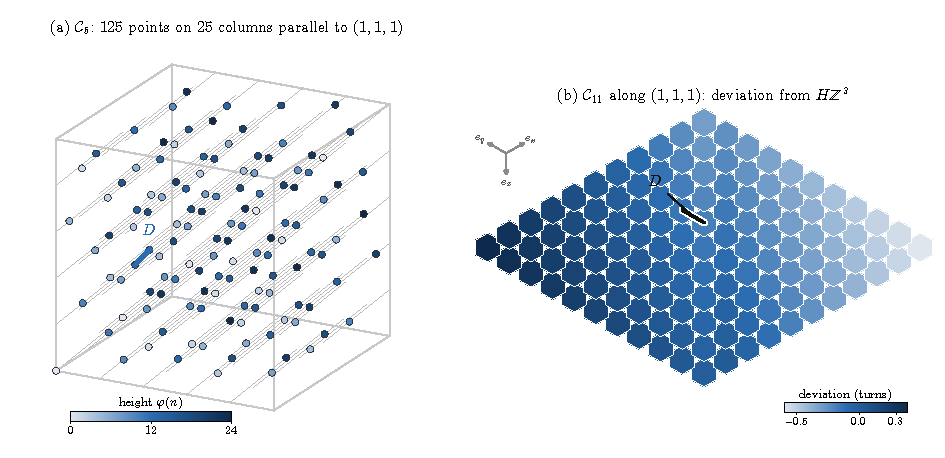
\includegraphics[width=\linewidth,height=0.5\textheight,keepaspectratio]{figs/col_net.pdf}}{\fbox{\parbox{0.9\textwidth}{\centering figure \texttt{col\_net} pending}}}
\caption{\colNetCaption\interactive{anatomy.html}}
\label{fig:col}
\end{figure}

\emph{Locally a reflected cube.} In cell units the point of cell $n$ is $n+\frac{\varphi([n])}{q^2}\mathbf 1$: it lies on the body diagonal of its cell. As $a/q=\frac13\mathbf 1+\frac1{3q}w$, two points whose cells differ by a bounded $E$ differ, in cell units, by
\[
E+\Bigl(\frac{\Sigma E}3+z+\frac{w\cdot E}{3q}\Bigr)\mathbf 1+\frac{\Delta j}{q^2}\mathbf 1
\]
for an integer $z$ (the wrap of $r$) and the change $\Delta j\in(-q,q)$ of the third digit. This is an $O(1/q)$ perturbation, \emph{along} $\mathbf 1$, of the point $E+\frac{z'}3\mathbf 1$, $z'=\Sigma E+3z$, of the set $\{E+\frac{z'}3\mathbf 1:z'\equiv\Sigma E\pmod3\}=H\Z^3$, where $H=I-\frac23\mathbf 1\mathbf 1^{\!\top}$ (for $v=E-\frac{z'+2\Sigma E}3\mathbf 1$ one checks $Hv=E+\frac{z'}3\mathbf 1$). Here $-H$ is the rotation by $180^\circ$ about the main diagonal, so $H\Z^3=-H\Z^3$ is the cubic lattice turned half a turn about $\mathbf 1$; we call it the \emph{reflected cube}. It has covolume $1$, minimum $1$ and minimal vectors $\pm H\e_c=\pm(\e_c-\frac23\mathbf 1)$.

\emph{Stacking.} Seen along $\mathbf 1$, both $\Z^3$ and $H\Z^3$ are the triangular lattice $\Pi_\perp\Z^3$ (a copy of $A_2$) with lines of points of period $\sqrt3$ over each site. In $\Z^3$ the line over the neighbour $\Pi_\perp\e_i$ is raised by $\frac13$ of the period, in $H\Z^3$ by $\frac23$, i.e.\ lowered by $\frac13$ (in crystallographic terms, the stackings $ABC$ and $ACB$ of triangular planes). If neighbouring columns had equal heights (the stacking $AA$), points would be only $\sqrt{2/3}$ apart. In the notation of Theorem~\ref{thm:colmin}, the height steps of $\Z^3$ and of $H\Z^3$ are $\Delta\equiv0$ and $\Delta\equiv\frac13q^2\pmod{q^2}$, both at distance $\frac13q^2$ from this worst step $\frac23q^2$; the theorem measures every step by its distance from it.

\emph{Drift and jitter.} The two perturbations are a \emph{drift} $\frac{w\cdot E}{3q}$, linear in $E$ and zero on $\mathbf 1$, and a \emph{jitter} $\Delta j/q^2$ of the third digit. Both are along $\mathbf 1$, so the columns are exact and only the heights deviate from the ideal, by $O(1/q)$. Section~\ref{sec:drift} shows that the losses $\frac1{3q}$ and $\frac2{3q}$ of Theorem~\ref{thm:col}(2) are forced, and that $\mathcal C_q$ is optimal among all column nets: going once around the torus along an axis takes $q$ steps, the ideal step of $H\Z^3$ is a third of the period, and $q/3$ is not an integer when $3\nmid q$, so the heights must deviate somewhere. Globally the set is not a lattice, since $qH\e_c\notin\Z^3$: at the wraps of $r$ the points jump back into their cells, and these are the slip planes of the column nets (Figure~\ref{fig:arclarge}). The drift vanishes on $\mathbf 1$ because $a\cdot\mathbf 1=q$, the condition that $q$ steps along $\mathbf 1$ close up; this is what makes $r$ a function of the column.

\begin{figure}[tbp]
\centering
\arcfig{arc_large}
\caption{\arcLargeCaption}
\label{fig:arclarge}
\end{figure}

The column structure is special to $m=3$. The following box count, which holds for every net, digital or not, shows that at every other resolution not even two coordinates can share the first offset digit (the geometric digit).

\begin{lemma}[Shared digits]\label{lem:shared}
Let $P$ be a $(0,m,s)$-net in base $q$, digital or not, $j\ge0$, and $a\ne b$ two coordinates. If $2(j+1)\le m$, then the pair of the digits with index $j$ of $a$ and of $b$ takes every value in $\{0,\dots,q-1\}^2$ at exactly $q^{m-2}$ points of $P$. In particular, if $f$ is a map of digits such that for every point of $P$ the digit with index $j$ of coordinate $b$ equals $f$ of the digit with index $j$ of coordinate $a$, then $2(j+1)>m$.
\end{lemma}

\begin{proof}
Let $2(j+1)\le m$ and choose the depths $d_a=j+1$, $d_b=m-j-1\ge j+1$ and $d_c=0$ for the other coordinates. Prescribing the digits $0,\dots,j$ of $a$ and of $b$ fixes the coordinate $a$ of an elementary box of this shape and the first $j+1$ digits of its coordinate $b$, and leaves $q^{m-2(j+1)}$ choices for the other digits of $b$; by $t=0$ each such box holds exactly one point. So each prescription is met by $q^{m-2j-2}$ points, and each value of the pair of digits with index $j$ by $q^{2j}\cdot q^{m-2j-2}=q^{m-2}$ points. A map $f$ as stated would leave the values $(\alpha,\beta)$, $\beta\ne f(\alpha)$, unmet.
\end{proof}

For $s=3$ and $m=3k$ the geometric digit has the index $k$, and $2(k+1)>3k$ only for $k=1$; so for $k\ge2$ no two coordinates of a $(0,3k,3)$-net can read the same geometric digit, let alone all three, and column nets exist only at $m=3$. At the other resolutions $m\ge4$ the lemma likewise excludes two coordinates that agree at the digit with index $\lfloor m/3\rfloor$, since $2(\lfloor m/3\rfloor+1)\le m$. So once $2(j+1)\le m$ the lemma excludes every relation between the digits with index $j$ of two coordinates, functional or not; it says nothing about relations among three coordinates, such as the rank-one layers of Section~\ref{sec:wnet} (Remark~\ref{rem:open}(7)).

At $m=3$ the third digit does not matter at first order: with the shared second digit of a reflected-cube layer and an arbitrary third digit in each coordinate, $\delta N^{1/3}=1-O(1/q)$.

\begin{proposition}[Arbitrary third digits]\label{prop:colfree}
Let $q\ge2$, let $w\in\Z^3$ with $w_x+w_y+w_z=0$ and $w_c\equiv-q\pmod3$, $a=\frac13(q\mathbf 1+w)$, and $\beta\in\Z$. Let $P$ be a set of $q^3$ points of the torus $(\Z/q^3\Z)^3$, one for each cell $n\in\{0,\dots,q-1\}^3$, at
\[
X(n)=q^2n+q\,r(n)\mathbf 1+j(n),\qquad r(n)\in[0,q),\ \ r(n)\equiv a\cdot n+\beta\pmod q,\qquad j(n)\in[0,q)^3
\]
(integers; $j$ arbitrary). Then any two distinct points of $P$ have toroidal distance at least $q^2-\bigl((\|w\|_1+3)q-3\bigr)/\sqrt3$.
\end{proposition}

\begin{proof}
Let $n\ne n'$ and let $D=q^2E+q\,\Delta r\,\mathbf 1+\Delta j$ be a representative of $X(n')-X(n)$ modulo $q^3$, with an integer vector $E\equiv n'-n\pmod q$, $\Delta r\in(-q,q)$ and $\Delta j\in(-q,q)^3$. If some $|E_c|\ge2$, then $|D_c|\ge2q^2-q(q-1)-(q-1)>q^2$. So let $E\in\{-1,0,1\}^3\setminus\{0\}$ and $\Sigma E=E_x+E_y+E_z$. The constant $\beta$ cancels: $\Delta r\equiv a\cdot E\pmod q$, and $3a\cdot E=q\Sigma E+w\cdot E$, so $3\Delta r=w\cdot E+zq$ with an integer $z\equiv\Sigma E\pmod3$. Hence $v=E-\frac{z+2\Sigma E}3\mathbf 1$ is an integer vector with $Hv=E+\frac z3\mathbf 1$, and
\[
3D=3q^2E+q\,(w\cdot E+zq)\mathbf 1+3\Delta j=3q^2Hv+R,\qquad R=q\,(w\cdot E)\mathbf 1+3\Delta j,
\]
with $|R_c|\le q\|w\|_1+3(q-1)$, since $|w\cdot E|\le\|w\|_1$. If $v\ne0$, then $|D|\ge q^2|Hv|-|R|/3\ge q^2-\bigl((\|w\|_1+3)q-3\bigr)/\sqrt3$, as $H$ is orthogonal. If $v=0$, then $E=t\mathbf 1$ with $3t=z+2\Sigma E=z+6t$, so $z=-3t$ and, as $w\cdot\mathbf 1=0$, $\Delta r=-tq$; then $|\Delta r|<q$ forces $t=0$, i.e. $E=0$, a contradiction.
\end{proof}

For $\mathcal C_q$, $\|w\|_1=4$, and the bound is $\delta N^{1/3}\ge1-(7q-3)/(\sqrt3q^2)$ whatever the third digits. The constant $\beta$ is what a digital shift with equal second digits in the three coordinates adds to the shared digit; since $\beta$ is arbitrary, the proposition also covers these shifts. Shifts whose second digits differ change the picture:

\begin{proposition}[Every digital shift at $m=3$]\label{prop:colshift}
Let $q\ge5$ with $\gcd(q,6)=1$, let $\tau$ be a digital shift of $\mathcal C_q$ (Definition~\ref{def:dshift}) with the digits $\tau_{c,1},\tau_{c,2},\tau_{c,3}$ in coordinate $c$ (the first, second and third digit), and put $W=2$ if $q\equiv2$ and $W=4$ if $q\equiv1\pmod3$ ($W/(3q)$ is the largest distance of $a_i/q$ or $2a_i/q$ from $\frac13$ or $\frac23$ that occurs; see the proof), and $a_{\max}=\max_ca_c$. The toroidal minimum distance of $\mathcal C_q\oplus\tau$ satisfies:
\begin{enumerate}
\item if $\tau_{x,2}=\tau_{y,2}=\tau_{z,2}$ and $\tau_{x,3}=\tau_{y,3}=\tau_{z,3}$, it equals that of $\mathcal C_q$ (Theorem~\ref{thm:col}(2));
\item if $\tau_{x,2}=\tau_{y,2}=\tau_{z,2}$, then $\delta N^{1/3}\ge1-(7q-3)/(\sqrt3q^2)$;
\item for every $\tau$,
\[
\delta N^{1/3}\ \ge\ \frac1{\sqrt3}\Bigl(1-\frac{W+3}q+\frac3{q^2}\Bigr),
\]
which exceeds $0.4693$ for every $q\ge37$; and if $\tau_{x,2},\tau_{y,2},\tau_{z,2}$ are not all equal, then $\delta N^{1/3}\le\sqrt3\,(q\,a_{\max}+q-1)/q^2=\frac1{\sqrt3}\bigl(1+\frac{3+w_{\max}}q-\frac3{q^2}\bigr)$, $w_{\max}=\max_cw_c$.
\end{enumerate}
The lower bounds of (2) and (3), and the value of (1) as a lower bound, hold for the Euclidean minimum distance too, which is at least the toroidal one; so does the upper bound of (3), which is witnessed by a pair that does not wrap.
\end{proposition}

\begin{proof}
\emph{Shifted digits.} By Lemma~\ref{lem:shift}, after re-indexing by the cells, the point of cell $n$ of $\mathcal C_q\oplus\tau$ has, in coordinate $c$, the digits $n_c$, $r_c(n)\equiv a\cdot n+\beta_c$ and $j_c(n)\equiv b\cdot n+\beta'_c$ with $\beta_c=\tau_{c,2}-a\cdot\tau_1$ and $\beta'_c=\tau_{c,3}-b\cdot\tau_1$, $\tau_1=(\tau_{x,1},\tau_{y,1},\tau_{z,1})$. So the $\beta_c$ are congruent if and only if the $\tau_{c,2}$ are equal, and likewise for $\beta'_c$ and $\tau_{c,3}$.

(1) Then $X(n)=q^2n+\varphi'([n])\mathbf 1$ with $\varphi'=q\,r+j$, $r=(a\cdot n+\beta)\bmod q$, $j=(b\cdot n+\beta')\bmod q$: a column point set. The map $[n]\mapsto(r,j)$ is still a bijection onto $(\Z/q\Z)^2$, so in the proof of Theorem~\ref{thm:col}(2) the same values $\Delta_i$ occur, and Theorem~\ref{thm:colmin} gives the same $d$.

(2) Proposition~\ref{prop:colfree} with $\|w\|_1=4$.

(3) \emph{Lower bound.} Let $n\ne n'$ and $D=q^2E+q\,\Delta r+\Delta j$ a representative, now with $\Delta r=(\Delta r_c)_c\in(-q,q)^3$. If some $|E_c|\ge2$, then $|D_c|>q^2$. So let $E\in\{-1,0,1\}^3\setminus\{0\}$, and let $\vartheta\in[0,q)$ be the residue of $a\cdot E$. The constants $\beta_c$ cancel: $\Delta r_c\equiv a\cdot E$ and $|\Delta r_c|<q$, so $\Delta r_c=\vartheta-q\omega_c$ with $\omega_c\in\{0,1\}$ ($\omega=0$ if $\vartheta=0$). Hence $D=q^2u+\Delta j$ with $u=E-\omega+\theta\mathbf 1$, $\theta=\vartheta/q$, and $|D|\ge q^2|u|-\sqrt3(q-1)$. Every $u_c$ lies in $\theta+\Z$, so $|u_c|\ge\|\theta\|$, the distance from $\theta$ to the nearest integer, and $\theta\equiv(a\cdot E)/q\pmod1$. If $\Sigma E=0$, then $E=\pm(\e_c-\e_d)$, the two moving coordinates of $u$ are $\pm(\theta+\{0,1\})$ and $\pm(\theta-\{1,2\})$, and $|u|^2\ge\theta^2+(1-\theta)^2\ge\frac12$. If $E=\pm\mathbf 1$, then $\vartheta=0$ and $|u|=\sqrt3$. Otherwise, up to sign, $E=\e_i$ or $E=\mathbf 1-2\e_i$ or $E=\mathbf 1-\e_i$, with $a\cdot E\equiv a_i$, $-2a_i$, $-a_i$ respectively. As $3a_i=q+w_i$ with $0<a_i<\frac q2$, $\|a_i/q\|=\frac{q+w_i}{3q}$ and $\|2a_i/q\|=\min\bigl(\frac{q-2w_i}{3q},\frac{2q+2w_i}{3q}\bigr)$; over the entries $w_i\in\{-2,1\}$ resp.\ $\{-1,2\}$ the least of these is $\frac{q-W}{3q}$. So $|u|\ge\sqrt3\,\|\theta\|\ge(q-W)/(\sqrt3q)$ in these cases, which is also less than $\frac1{\sqrt2}$ and $\sqrt3$. Therefore $|D|\ge q(q-W)/\sqrt3-\sqrt3(q-1)=\bigl(q^2-(W+3)q+3\bigr)/\sqrt3$ for every pair, which is the bound. It increases with $q$ within each residue class; for $q\ge37$ its least value is $0.4693\ldots$ at $q=37$ ($W=4$), and $0.5079\ldots$ at $q=41$ in the class $W=2$.

\emph{Upper bound.} Put $b_c\equiv-\beta_c\pmod q$; they are not all equal. Along $\e_c$ the shared digit changes by $a_c$, and $r_d$ wraps if and only if $\vartheta=a\cdot n\bmod q$ lies in the cyclic interval $J^{(c)}_d=\{b_d-a_c,\dots,b_d-1\}$ of $a_c$ consecutive residues of $\Z/q\Z$. We find $c$ and a residue $\vartheta$ that lies in $J^{(c)}_c$ and in no $J^{(c)}_d$, $d\ne c$. If the $b_d$ are distinct, let $g_c\ge1$ be the distance from $b_c$ forward around $\Z/q\Z$ to the next of them. The gaps sum to $q=a_x+a_y+a_z$, so $g_c\ge a_c$ for some $c$; then $\vartheta=b_c-1$ lies in $J^{(c)}_c$, and it lies in $J^{(c)}_d$ only if $b_d$ is at forward distance at most $a_c-1$ from $b_c$, which no $b_d$ is. If exactly two of them are equal, $b_d=b_{d'}\ne b_c$, then $J^{(c)}_c$ and $J^{(c)}_d=J^{(c)}_{d'}$ are two different cyclic intervals of the same length $a_c<q$, so neither contains the other. Take a cell $n$ with $n_c=0$ and $a\cdot n\equiv\vartheta$ (possible, as the entries $a_d$, $d\ne c$, are units) and $n'=n+\e_c$, so that the pair does not wrap in the cell digits. Then $\Delta r_c=a_c-q$ and $\Delta r_d=a_c$ for $d\ne c$, so the representative with $E=\e_c$ is $D=q^2\e_c+q(a_c\mathbf 1-q\e_c)+\Delta j=q\,a_c\mathbf 1+\Delta j$, and $|D|\le\sqrt3\,(q\,a_{\max}+q-1)$.
\end{proof}

So the exact minimum distance of $\mathcal C_q$ survives exactly the digital shifts whose digits agree in the three coordinates on the two shared digits, the first-order value $1$ survives those that agree on the geometric digit, and the others give $1/\sqrt3$ at first order. Unequal second shift digits make the three coordinates wrap at different cells, so the shared digit no longer moves all three coordinates together, and a step across a wrap of one coordinate alone is short; Remark~\ref{rem:glue} explains why the value then drops to $1/\sqrt3$. The constants of Corollary~\ref{cor:allm} below survive every shift (Section~\ref{sec:dgs}).
\subsection{\texorpdfstring{$m\equiv1,2$}{m = 1, 2}: lattice skeletons}\label{sec:allm}
For $s=3$ the residue $m\equiv2$ ($\ell=1$ skeleton coordinate) is the case $s=3$ of Theorem~\ref{thm:S1}. The residue $m\equiv1$ ($\ell=2$ skeleton coordinates, $r=1$) needs a different lattice, since Theorem~\ref{thm:S2} needs $s\ge4$: here the occupied fine cells form, in each coarse block, a coset of the Korobov lattice with generating vector $(1,\rho,\rho^2)$ modulo $p$. We realize both on the M\"obius frame $(\Psi^2,I,\Psi)$ of Section~\ref{sec:frames} (Definition~\ref{def:net} used $T=\pm\Psi$; the sign does not matter here). It is defined for every $m$, and the proof of Theorem~\ref{thm:t0} does not use $3\mid m$ (only (F1), (F2) and $\Psi^3=\pm1$), so all its box minors are $\pm1$ and it has an integer graph form $\Phi^F$ with depths $\mathbf k$.

\emph{Notation.} The \emph{column block} $x$ consists of the blocks $\Phi_{cx}$, $c\in\{x,y,z\}$, which multiply the cell index $n_x$; its columns are the levels $x_l$, $0\le l<k_x$, of $n_x$ (level $l$ of $n_x$). We write $Y0|x_l$ for the entry of the first offset row of $y$ on the level $l$ of $n_x$, and so on, and ``box $(d_x,d_y,d_z)$'' for the elementary box with these depths. We modify $\Phi^F$ modulo $p$ by the moves of Lemma~\ref{lem:box}: inside a column block, adding multiples of less significant levels to a level or scaling a level by a unit (move (c)); scaling single off-diagonal blocks (move (b)); and setting diagonal blocks (move (a)). Every pivot used below is a nonzero entry or $2\times2$ minor, because by Lemma~\ref{lem:box} it is the box minor of the frame for the box indicated, which is $\pm1$.

\begin{definition}\label{def:B}
Let $\rho$ be an integer with $\rho\not\equiv0\pmod p$.
\begin{enumerate}
\item[($\mathcal B^2$)] $\mathbf k=(k+1,k+1,k)$; the recipe of Proposition~\ref{prop:skelcomp}(ii) with $\kappa=(\rho,\rho^2)$. In column block $x$: $Z0|x_k\ne0$ (box $(k,k+1,k+1)$); subtract multiples of level $x_k$ from every level $x_l$, $l<k$, so that $Z0|x_l=0$, then scale level $x_k$ so that $Z0|x_k=\rho$. In column block $y$ the same, with pivot $Z0|y_k$ (box $(k+1,k,k+1)$) and target $\rho^2$. Set all diagonal blocks to $0$. The result is the digital net $\mathcal B^2_{k,p,\rho}$ over $\F_p$; its skeleton digit is
\[
S_z\equiv\rho\,x_k+\rho^2\,y_k\pmod p.
\]
\item[($\mathcal B^1$)] $\mathbf k=(k+1,k,k)$. The goal is a graph form whose skeleton digits are $S_y\equiv\rho x_k+z_{k-1}$ and $S_z\equiv\rho^2x_k+x_{k-1}+y_{k-1}-z_{k-1}\pmod p$, with every box minor a unit; the steps are as follows. Column block $x$: the matrix $\left(\begin{smallmatrix}Y0|x_k&Y0|x_{k-1}\\ Z0|x_k&Z0|x_{k-1}\end{smallmatrix}\right)$ is invertible (box $(k-1,k+1,k+1)$); call its determinant $\Delta$; use the levels $x_k$, $x_{k-1}$ to make $Y0$ and $Z0$ vanish on the levels $l<k-1$; then add a multiple of $x_k$ to $x_{k-1}$ so that $Y0|x_{k-1}=0$. Now $Y0|x_k\ne0$ (box $(k,k+1,k)$), $Z0|x_k\ne0$ (box $(k,k,k+1)$) and $Z0|x_{k-1}=\Delta/Y0|x_k\ne0$. Scale the block $\Phi_{zx}$ so that $Z0|x_{k-1}=1$, the level $x_k$ so that $Z0|x_k=\rho^2$, and the block $\Phi_{yx}$ so that $Y0|x_k=\rho$. Column block $y$: with the pivot $Z0|y_{k-1}\ne0$ (box $(k+1,k-1,k+1)$) make $Z0|y_l=0$ for $l<k-1$ and scale $\Phi_{zy}$ so that $Z0|y_{k-1}=1$. Column block $z$: the same for $Y0|z$ (box $(k+1,k+1,k-1)$). Diagonal blocks: $Z0|z_{k-1}=-1$ and all other entries $0$. The result is $\mathcal B^1_{k,p,\rho}$; its skeleton digits are
\[
S_y\equiv\rho\,x_k+z_{k-1},\qquad S_z\equiv\rho^2\,x_k+x_{k-1}+y_{k-1}-z_{k-1}\pmod p.
\]
\end{enumerate}
\end{definition}

The levels and blocks not mentioned keep the values of $\Phi^F$ modulo $p$. Each net is obtained by finitely many explicit elementary operations on the explicit integer matrix $\Phi^F$, and only the skeleton digits matter for the separation proofs below.

\begin{proposition}\label{prop:Bnet}
For every prime $p$, every $k\ge1$ and every $\rho\not\equiv0\pmod p$, $\mathcal B^2_{k,p,\rho}$ is a $(0,3k+2,3)$-net and $\mathcal B^1_{k,p,\rho}$ is a $(0,3k+1,3)$-net over $\F_p$.
\end{proposition}

\begin{proof}
Every box minor of $\Phi^F$ is $\pm1$, and each move multiplies every box minor by a unit of $\F_p$ (Lemma~\ref{lem:box}; the targets $\rho$, $\rho^2$, $1$ and the pivots are units). Lemma~\ref{lem:nie} completes the proof.
\end{proof}

\begin{figure}[tbp]
\centering
\arcfig{arc_skeleton}
\caption{\arcSkeletonCaption}
\label{fig:Blattice}\label{fig:arcskeleton}
\end{figure}

\begin{remark}[Dimension three, $m\equiv2\pmod3$]\label{rem:B2}
For $s=3$ the recipes of Definitions~\ref{def:S1} and~\ref{def:B}($\mathcal B^2$) coincide (Proposition~\ref{prop:skelcomp}(ii) with $\kappa=(\rho,\rho^2)$, skeleton digit $S_z=\rho x_k+\rho^2y_k$), and Theorem~\ref{thm:S1} uses only the skeleton digit. So for every prime $p$, every $k\ge1$ and every $\rho\ge1$ with $\rho^3<p$, $\mathcal B^2_{k,p,\rho}$ is a $(0,3k+2,3)$-net over $\F_p$ (Proposition~\ref{prop:Bnet}) with toroidal $\delta N^{1/3}\ge(\rho-1)\,p^{-1/3}$ (Theorem~\ref{thm:S1}(1) for $\rho\ge2$; the bound is $0$ for $\rho=1$); its occupied fine cells are exactly the cells of the index-$p$ lattice $\Lambda_{\mathcal B^2}=\{a:a_z\equiv\rho a_x+\rho^2a_y\pmod p\}$, of minimum $\rho$ (Theorem~\ref{thm:S1}(2), Figure~\ref{fig:Blattice}(a),~(b)); and for $\rho=\lfloor p^{1/3}\rfloor$ its mesh ratio is bounded uniformly in $p$ (Theorem~\ref{thm:S1}(3)). With $\rho$ maximal, $p<(\rho+1)^3$, so the bound exceeds $(\rho-1)/(\rho+1)$ and tends to $1$. It is a sawtooth in $p$ (it drops each time $\lfloor p^{1/3}\rfloor$ increases), first exceeds $0.9$ at $p=1361$, and stays above $0.9$ for every prime $p\ge6863$ ($\rho\ge19$). The bound is sharp for the method: the bound of Lemma~\ref{lem:skelred}(i), which allows a jitter of one fine cell in every coordinate, equals $(\rho-1)p^{-1/3}$ exactly, attained at the step $(-\rho,1,0)$.
\end{remark}

\begin{theorem}[Dimension three, $m\equiv1\pmod3$]\label{thm:allm}
Let $p$ be a prime, $k\ge1$, and let $\rho\ge2$ with $\rho^2(\rho+1)\le p$. The digital net $\mathcal B^1_{k,p,\rho}$ of Definition~\ref{def:B} is a $(0,3k+1,3)$-net over $\F_p$ whose toroidal minimum distance satisfies $\delta N^{1/3}\ge(\rho^2-4)\,p^{-2/3}$. With $\rho$ the largest integer such that $\rho^2(\rho+1)\le p$, the bound tends to $1$ as $p\to\infty$; it exceeds $0.9$ once $\rho\ge27$, i.e.\ $p\ge27^2\cdot28=20412$, so for every prime $p\ge20431$.
\end{theorem}

\begin{proof}[Proof of Theorem~\ref{thm:allm}]
The net property is Proposition~\ref{prop:Bnet}; the hypotheses give $2\le\rho<p$, so $\rho\not\equiv0$. Let $v\ne w$ be two points, $a\ne0$ the centred difference of their fine positions, and $M=|a|_\infty$. If $M\ge p-1$ we are done, since $p-1\ge\rho^2-3$. Otherwise let $\xi_c=\xi_{c,1}$ be the floor changes of Lemma~\ref{lem:skelred}(ii) and $u=(a_x,\ a_y-\xi_z,\ a_z-\xi_x-\xi_y+\xi_z)$. By the displayed relations, $u\in\Lambda_{\mathcal B^1}$, and $|u|_\infty\le M+3$. If $u\ne0$, Lemma~\ref{lem:skellat}(L1) gives $M+3\ge\rho^2$. If $u=0$, then $a_x=0$, hence $\xi_x=0$, $a_y=\xi_z$ and $a_z=\xi_y-\xi_z$. If $\xi_z=1$ then $a_z>0$, so $\xi_y\ge2$, impossible; if $\xi_z=-1$ then $a_z<0$ and $\xi_y\le-2$, impossible. So $\xi_z=0$, $a_y=0$, $\xi_y=0$ and $a_z=0$, contradicting $a\ne0$. Hence $M\ge\rho^2-3$, and Lemma~\ref{lem:skelred}(i) with $\ell=2$ gives $\delta N^{1/3}\ge(\rho^2-4)p^{-2/3}$.

\emph{Constants.} Let $c_1(p)=(\rho^2-4)p^{-2/3}$ be the bound with $\rho$ maximal. Then $p<(\rho+1)^2(\rho+2)$, hence
\[
c_1(p)^3>G(\rho)=\frac{(\rho-2)^3(\rho+2)}{(\rho+1)^4}.
\]
$G$ increases for $\rho\ge3$, since $(\log G)'=9/((\rho-2)(\rho+1))-1/((\rho+1)(\rho+2))$ is positive, and tends to $1$. Since $\rho\ge27$ iff $p\ge20412$, and $G(27)^{1/3}=0.9033\ldots$, the bound exceeds $0.9$ from this prime on.
\end{proof}

The case $u=0$ uses the own-coordinate term $-z_{k-1}$ of $S_z$: with $+z_{k-1}$ or $0$ there and equal signs of the faults this argument does not apply. Like that of Remark~\ref{rem:B2}, the bound is a sawtooth in $p$.

\emph{Lattice reading.} For $\mathcal B^1$ the skeleton digits give, with $P_c$ the fine cell of coordinate $c$ (Section~\ref{sec:fine}),
\[
P_y\equiv\rho P_x+\lfloor P_z/p\rfloor,\qquad P_z\equiv\rho^2P_x+\lfloor P_x/p\rfloor+\lfloor P_y/p\rfloor-\lfloor P_z/p\rfloor\pmod p,
\]
so inside each coarse block the occupied fine cells (one in $p^2$) form a coset of $\Lambda_{\mathcal B^1}$, the Korobov lattice with generating vector $(1,\rho,\rho^2)$ and modulus $p$ \cite{Kor59,SJ94}, shifted by unit \emph{faults} between neighbouring coarse blocks (Figure~\ref{fig:Blattice}(c)). The choice $\rho\approx p^{1/3}$ makes the shortest (primal) vector as long as possible for a lattice of index $p^2$, up to a constant (the pigeonhole bound after Lemma~\ref{lem:skelred}). For integration it would be a poor Korobov generator: $(\rho,-1,0)$ lies in the dual lattice, so its Zaremba index is at most $\rho$. Separation (primal) and integration (dual) favour different generators.


\subsection{Every resolution}\label{sec:everym}
Together, the nets of this section cover every resolution $m\ge3$ for every large prime.

\begin{corollary}[Every prime $p\ge37$, every $m\ge3$]\label{cor:allm}
For every prime $p\ge37$ and every $m\ge3$ the nets of Theorems~\ref{thm:col} ($m=3$), \ref{thm:main} ($m\equiv0$, $m\ge6$), \ref{thm:allm} ($m\equiv1$) and~\ref{thm:S1} with $s=3$ ($m\equiv2$; the nets $\mathcal B^2$ of Remark~\ref{rem:B2}), with $\rho$ maximal, are explicit digital $(0,m,3)$-nets over $\F_p$ with
\[
\delta N^{1/3}>0.2715,\quad\text{and}\quad\delta N^{1/3}>0.4250\ \text{if } p\ge83,
\]
uniformly in $m$, and the lower bound tends to $1$ as $p\to\infty$. Their covering radius satisfies $hN^{1/3}\le\sqrt3$ for $m\equiv0$, $hN^{1/3}\le p^{1/3}\sqrt{2+p^{-2}}$ for $m\equiv1$, and $hN^{1/3}\le\min\{p^{2/3}\sqrt{1+2p^{-2}},\,4.264\}$ for $m\equiv2\pmod 3$. So for each such $p$ the mesh ratio $h/\delta$ is bounded uniformly in $m$: the nets are quasi-uniform along every $N=p^m$, $m\ge3$. For $m\equiv2$ the mesh ratio is moreover at most $7\sqrt3<12.2$ for every prime $p\ge11$ and every $m\ge5$ (Theorem~\ref{thm:S1}(3)).
\end{corollary}

\begin{proof}[Proof of Corollary~\ref{cor:allm}]
Take $\mathcal C_p$ for $m=3$ (Theorem~\ref{thm:col}; for $p\ge37$, $\delta N^{1/3}>0.9823$, and its covering radius is at most $\sqrt3N^{-1/3}$ because every cell holds a point), $\mathcal P_{k,p}$ for $m=3k\ge6$, $\mathcal B^1_{k,p,\rho}$ for $m=3k+1\ge4$ and $\mathcal B^2_{k,p,\rho}$ for $m=3k+2\ge5$, with $\rho$ maximal: $\rho_1$ and $\rho_2$, the largest integers with $\rho_1^2(\rho_1+1)\le p$ and $\rho_2^3<p$. For $p\ge37$, $\rho_1\ge3$ and $\rho_2\ge3$. If $37\le p\le79$ then $\rho_1=3$ and the bound of $\mathcal B^1$ is $5p^{-2/3}\ge5\cdot79^{-2/3}=0.27157\ldots$, the bound of $\mathcal B^2$ is $\ge2\cdot61^{-1/3}>0.508$, and $1-1/p>0.97$. If $p\ge83$ then $\rho_1\ge4$ and $\rho_2\ge4$, and the bounds exceed $G(4)^{1/3}=(48/625)^{1/3}>0.4250$ and $(\rho-1)/(\rho+1)=3/5$ at $\rho=4$ (Remark~\ref{rem:B2}). All bounds tend to $1$. For the covering radius: by $t=0$ the elementary box with depths $\mathbf k$ (resp. $(k,k,k)$) around any point of the torus contains a net point, and its diagonal is $p^{-k}\sqrt{2+p^{-2}}=p^{1/3}\sqrt{2+p^{-2}}\,N^{-1/3}$ for $m\equiv1$ and $p^{-k}\sqrt{1+2p^{-2}}=p^{2/3}\sqrt{1+2p^{-2}}\,N^{-1/3}$ for $m\equiv2$. For $m\equiv2$, Theorem~\ref{thm:S1}(3) with $s=3$ gives $hN^{1/3}\le\sqrt3(\mu+1)p^{-1/3}$ and $h/\delta\le\sqrt3(\mu+1)/(\rho-1)$, $\mu=\lceil p/\rho^2\rceil$; over all primes $p\ge11$ the maxima are $4.2633\ldots<4.264$ and $7\sqrt3$, both at $p=23$ (for $\rho\ge4$ use $\mu<\rho(1+1/\rho)^3+1$).
\end{proof}

For $m\equiv1$ the mesh ratio obtained in this way grows like $p^{1/3}$. Whether a bound uniform in $p$ holds is open (Remark~\ref{rem:open}(5); for $m\equiv2$ it is Theorem~\ref{thm:S1}(3)). (Heuristic for one: the cosets of $\Lambda_{\mathcal B^1}$ have reduced bases of about $\rho^2$ fine cells, i.e. $O(N^{-1/3})$; a proof has to handle the faults between coarse blocks, and we have not given one.) The separation bounds and the lattice reading use only the skeleton digits: the bounds of Theorem~\ref{thm:allm} hold for every graph form over $\F_p$ with the depths $\mathbf k$ and the skeleton digits of Definition~\ref{def:B}, net or not.

At $m=3$ the constant can exceed $1$ (Part~II). If two coordinates share the geometric digit and the third reads it with the factor $\frac12$ modulo $p$, the points lie locally on two cosets of a lattice, with the limit $\sqrt{66}/8=1.0155\ldots$ (Proposition~\ref{prop:twocoset}). If all three geometric digits are multiples of one digit, the three coordinates wrap together, and $\delta N^{1/3}>1$ for every prime $p\ge17$, with the limit $\sqrt{281}/16=1.0476\ldots$ (Proposition~\ref{prop:wnet}). For small primes, the per-prime nets of Remark~\ref{rem:perprime} give larger constants and close most of the remaining gaps:

\begin{remark}[Per-prime designs]\label{rem:perprime}
For small primes, computer-found designs give larger constants. They are graph forms with the depths $\mathbf k$, built by the same moves from the frame, in which the skeleton digits and the next offset digit of each coordinate (which controls the jitter) are prescribed on the last three or four levels; their skeletons are index-$p^2$ Korobov-type ($m\equiv1$) and index-$p$ congruence lattices ($m\equiv2$). A finite computation analogous to Lemma~\ref{lem:Ss} (it enumerates the steps between nearby fine cells, all carry patterns and both representatives of each digit difference) certifies the constants of Table~\ref{tab:perprime} for every $m=3k+1\ge10$ resp. $m=3k+2\ge8$, since the prescribed rows do not depend on $k$; they exceed $1$ for $p=47$, $53$, $59$, $61$, $71$, $73$, $79$ ($m\equiv1$) and $p=41$, $43$, $59$, $61$, $79$ ($m\equiv2$). This separation bound is Proposition~\ref{prop:ppsep}, and it holds for every digital shift as well (Remark~\ref{rem:ppshift}). The existence of such a $(0,m,3)$-net for every $k$ (Propositions~\ref{prop:pp2} and~\ref{prop:pp1}, Appendix~\ref{app:perprime}) rests on quantities that the moves of Lemma~\ref{lem:box} do not change and that do not depend on $k$ (Lemma~\ref{lem:ppinv}: five for $m\equiv1$, two for $m\equiv2$), and on finitely many exact checks per design (proofs in Appendix~\ref{app:perprime}; formalization status in Section~\ref{sec:formal}).
\end{remark}

Together these results give, for every prime $p\ge5$, explicit digital $(0,m,3)$-nets over $\F_p$ at the following resolutions. At $m=3$, Theorem~\ref{thm:col} gives $\delta N^{1/3}>0.9059$, and Theorem~\ref{thm:main} covers every $m\equiv0$, $m\ge6$. For $m\equiv1$, $m\ge10$, $\delta N^{1/3}>0.4250$ (Theorem~\ref{thm:allm}, and for $p\le79$ the per-prime certificates of Remark~\ref{rem:perprime}). For $m\equiv2$, $m\ge8$, $\delta N^{1/3}>0.5$ (Remark~\ref{rem:B2}, and for $p\le79$ the per-prime certificates); for $p\ge11$ the nets $\mathcal B^2$ of Remark~\ref{rem:B2} also cover $m=5$. Not covered are $m\in\{4,7\}$ for $5\le p\le31$ and $m=5$ for $p\le7$; finitely many resolutions do not matter for the question of Dick, Goda and Suzuki (Remark~\ref{rem:dgsfinite}). In the bases $2$ and $3$ every $m$ is covered (Theorem~\ref{thm:base23}).

\section{Bases two and three: the deep-shift lift}\label{sec:base23}
The constructions so far need large bases. The net of Theorem~\ref{thm:main} is a $(0,3k,3)$-net in every base, but its separation bound needs $q\ge4$; the other residues need large primes (Corollary~\ref{cor:allm}). The bases two and three, the most common ones in practice, need another idea.

\begin{remark}[Why $s=3$, and base two]\label{rem:base2}
A $(0,m,s)$-net in base $2$ with $m\ge2$ requires $s\le3$ \cite[Cor.~5.11]{Nie87}; for digital nets over rings see \cite[Thm.~2]{LNS96}. So $s=3$ is the largest dimension in which one set of integer generator matrices can give $t=0$ in every base (for dimension $s$ see the text after Lemma~\ref{lem:Ts}). In the frame language of Section~\ref{sec:frames}: $t=0$ in every base needs places whose pairwise differences are $\pm1$; $\{0,1\}$ is the largest set of integers with this property (in the language of exceptional units \cite{Len77}), and the place $\infty$ gives the third coordinate.
\end{remark}

In base $b\in\{2,3\}$ we therefore build the nets recursively, $m\to m+3$, from a finite seed. Each step adds one digit at the top of every coordinate and two at the bottom. The three new top digits form a $(0,3,3)$-net in base $b$, so they split the cube into $b^3$ \emph{top boxes} of side $1/b$. Every top box receives a copy of the old net, and the two new bottom digits are jitter. Neighbouring copies differ by digital shifts that change only the lower half of the old digits. The upper half of every old point therefore never changes (it is \emph{frozen}), and the separation that the old net has at the scale of its upper half survives every later step. This is the mechanism of the introduction again, with the old net in the role of the lattice and the shifted lower digits as jitter (Figure~\ref{fig:base23}).

\emph{Setting.} Let $b$ be a prime and $m_0\ge1$. A digitally shifted digital $(0,m_0,3)$-net over $\F_b$ is a set $P=\{\xi(n)=Cn+\tau:n\in\F_b^{m_0}\}$ with $C=(C_x,C_y,C_z)$, $C_c\in\F_b^{m_0\times m_0}$, and a shift $\tau\in\F_b^{3m_0}$; a point has the three digit vectors $\xi_c(n)\in\F_b^{m_0}$, most significant digit first. For a pair of coordinates $(c,c')\in\{(y,z),(x,y),(x,z)\}$ let $P_{cc'}=\{(C_cn,C_{c'}n):n\in\F_b^{m_0}\}\subset\F_b^{m_0}\times\F_b^{m_0}$, an $m_0$-dimensional subspace (a digital $(0,m_0,2)$-net). For $1\le e\le m_0$ let $Z_e\subset\F_b^{m_0}\times\F_b^{m_0}$ be the vectors that vanish on the first $e$ digits of $c$ and on the first $m_0+1-e$ digits of $c'$. Since the map from $P_{cc'}$ to the first $e$ digits of $c$ and the first $m_0-e$ digits of $c'$ (the box of shape $(e,m_0-e)$) is injective, $P_{cc'}\cap Z_e=0$, so $H_e=P_{cc'}\oplus Z_e$ is a hyperplane; let $\lambda^{cc'}_e$ be a nonzero linear functional with kernel $H_e$. A point of $P_{cc'}+t\,s$, $t\ne0$, and a point of $P_{cc'}$ fall into the same elementary box of shape $(e,m_0+1-e)$ only if $s\in H_e$; so $\lambda^{cc'}_e(s)\ne0$ says that adding multiples of $s$ to the pair $(c,c')$ creates no collision in boxes of that shape.

\begin{definition}[Deep-shift lift]\label{def:lift}
Let $P$ be as above, $0\le D$, and let $s_A,s_B\in\F_b^{3m_0}$ vanish on the first $D$ digits of each coordinate, i.e.\ change only the \emph{deep} digits, those of index $>D$. They are \emph{separating} if, for every $1\le e\le m_0$,
\[
\lambda^{yz}_e\bigl(s_A^{yz}\bigr)\ne0,\qquad \lambda^{xy}_e\bigl(s_B^{xy}\bigr)\ne0,\qquad \lambda^{xz}_e\bigl((s_B-s_A)^{xz}\bigr)\ne0,
\]
where $s^{cc'}$ is the restriction of $s$ to the coordinates $c,c'$. The \emph{lift} $L_D(P)$ is the set of $b^{m_0+3}$ points with index $(n,\alpha,\beta_1,\beta_2)\in\F_b^{m_0+3}$ whose coordinates have the $m_0+3$ digits
\[
\begin{aligned}
x&:\ \alpha\ \bigm|\ (\xi(n)+s_\beta)_x\ \bigm|\ \beta_2,\ \beta_1,\\
y&:\ \alpha+\beta_1\ \bigm|\ (\xi(n)+s_\beta)_y\ \bigm|\ \beta_1+\beta_2,\ \beta_1,\\
z&:\ \alpha+\beta_1+\beta_2\ \bigm|\ (\xi(n)+s_\beta)_z\ \bigm|\ \beta_1,\ \beta_2,
\end{aligned}
\qquad s_\beta=\beta_1s_A+\beta_2s_B,
\]
one \emph{top} digit, $m_0$ \emph{block} digits and two \emph{jitter} digits. The shift $\tau$ of $P$ stays in the block digits, so $L_D(P)$ is again a digitally shifted digital net over $\F_b$.
\end{definition}

\begin{lemma}[Lift]\label{lem:lift}
Let $P$ be a digitally shifted digital $(0,m_0,3)$-net over $\F_b$.
\begin{enumerate}
\item[(A)] If $s_A,s_B$ are separating, then $L_D(P)$ is a digitally shifted digital $(0,m_0+3,3)$-net over $\F_b$.
\item[(B)] If $2D\le m_0$, separating $s_A,s_B$ exist.
\end{enumerate}
\end{lemma}

There are $m_0$ conditions for each pair of coordinates, one for each $e$. Each $\lambda_e$ involves a deep digit, and $2D\le m_0$ makes these deep digits distinct, so the conditions can be met independently.

\begin{proof}
(A) Let $(d_x,d_y,d_z)$ be a box shape with $\sum_cd_c=m_0+3$; by Lemma~\ref{lem:nie} it suffices that the box map, from the index to the prescribed digits, is injective. \emph{All $d_c\ge1$.} The top digits $(\alpha,\alpha+\beta_1,\alpha+\beta_1+\beta_2)$ determine $(\alpha,\beta)$. The remaining depths $d_c-1$ sum to $m_0$ and are at most $m_0$ each, so no jitter digit is prescribed, and what remains is an $m_0$-box of the shifted net $P+s_\beta$, which is injective. \emph{Exactly one $d_c=0$}, say $d_x=0$ (the cases $d_y=0$, $d_z=0$ are the same with the pairs $xz$ and $xy$). The top digits of $y$ and $z$ fix $\alpha+\beta_1$ and $\beta_2$, and the remaining index is $(n,t)$ with $t=\beta_1$; the block digits of $(y,z)$ are those of $P_{yz}+\text{const}+t\,s_A^{yz}$. If $d_y-1=e$ and $d_z-1=m_0+1-e$ with $1\le e\le m_0$, injectivity on $(n,t)$ is injectivity of the projection to the first $e$ resp.\ $m_0+1-e$ digits on $P_{yz}+\F_bs_A^{yz}$; it holds on $P_{yz}$ by the $(e,m_0-e)$ box, and for $t\ne0$ a collision would put $s_A^{yz}$ in $H_e=\ker\lambda^{yz}_e$, which the separating condition excludes. If $d_y=1$ or $d_z=1$, the other coordinate reads all of its block and one jitter digit, $\beta_1$ for $z$ and $\beta_1+\beta_2$ for $y$, which determines $t$, and then the block determines $n$. For $d_y=0$ the pair is $(x,z)$ with the line $s_B-s_A$ and the jitter digits $\beta_2$, $\beta_1$; for $d_z=0$ it is $(x,y)$ with $s_B$ and $\beta_2$, $\beta_1+\beta_2$. \emph{Two $d_c=0$.} One coordinate carries all $m_0+3$ digits: its top digit, its block (a bijection in $n$ for fixed $\beta=(\beta_1,\beta_2)$) and its two jitter digits, which are a bijection of $\F_b^2$ onto $(\beta_1,\beta_2)$ in every coordinate.

(B) The functional $\lambda_e=\lambda^{cc'}_e$ vanishes on $Z_e$, so it is supported on the first $e$ digits of $c$ and the first $m_0+1-e$ digits of $c'$. Its coefficient on digit $e$ of $c$ is nonzero: otherwise $\lambda_e$ would live on a window of $e-1$ plus $m_0+1-e$ digits, onto which $P_{cc'}$ projects bijectively (the $(e-1,m_0+1-e)$ box), and vanish on $P_{cc'}$, hence be $0$. Likewise its coefficient on digit $m_0+1-e$ of $c'$ is nonzero. If $e>D$, digit $e$ of $c$ is \emph{deep} (index $>D$); if $e\le D$, digit $m_0+1-e\ge m_0+1-D>D$ of $c'$ is deep. So each $\lambda_e$ has a nonzero coefficient on a deep digit, its own: digit $e$ of $c$ if $e>D$, digit $m_0+1-e$ of $c'$ if $e\le D$. In any vanishing linear combination, the term with the largest $e>D$ (or, if there is none, the smallest $e$) is the only one that sees its own digit, so its coefficient is $0$; by induction all coefficients are $0$. Hence the restrictions of $\lambda_1,\dots,\lambda_{m_0}$ to the deep digits are linearly independent, and the deep parts of $s_A^{yz}$ can be chosen with $\lambda^{yz}_e(s_A^{yz})=1$ for all $e$, those of $s_B^{xy}$ with $\lambda^{xy}_e(s_B^{xy})=1$; the conditions on $(s_B-s_A)^{xz}$ involve the still free deep digits of $(s_A)_x$ and $(s_B)_z$, and are solved in the same way.
\end{proof}

A \emph{deep-shift chain} is a sequence $P_{m_0}\to P_{m_0+3}\to\cdots$ of lifts $P_{\ell+3}=L_{D_\ell}(P_\ell)$ with $2D_\ell\le\ell$, where $P_\ell$ has $b^\ell$ points (the resolution $\ell$); its \emph{canonical continuation} from a resolution $\ell_0$ on uses $D_\ell=\lfloor\ell/2\rfloor$. For a resolution $L$ write $A=b^{\lfloor L/2\rfloor}$ (the number of values of the top $\lfloor L/2\rfloor$ digits) and $W=b^{L-\lfloor L/2\rfloor}$, read the coordinates of a point of $P_L$ as integers $X_c\in[0,b^L)$, and let $t_c=\lfloor X_c/W\rfloor$ be the integer of its top $\lfloor L/2\rfloor$ digits. Put
\[
v^*_L=\min_{p\ne p'\in P_L}\ \sum_{c}\max\bigl(0,\ |t_c(p)-t_c(p')|_{A}-1\bigr)^2,\qquad g_L=W\sqrt{v^*_L}\,b^{-2L/3},
\]
with $|\cdot|_A$ the distance to the nearest multiple of $A$; $v^*_L$ is an integer, computable from $P_L$ alone. It is the smallest squared toroidal distance between the top halves of two points of $P_L$, in units of $W$, after one unit per coordinate is subtracted for the unknown lower half; $g_L$ is the same quantity normalized like $\delta N^{1/3}$.

\begin{lemma}[Freezing and separation]\label{lem:liftsep}
Let $P_L\to P_{L+3}\to\cdots$ be lifts whose depth parameters satisfy $D_{L+3j'}\ge\lfloor L/2\rfloor+j'$ for every $j'\ge0$ (for instance the canonical continuation). Then for every $j\ge0$ the toroidal (hence also Euclidean) minimum distance of $P_{L+3j}$ satisfies
\[
\delta N^{1/3}\ \ge\ \min\bigl(g_L,\ b^{L/3}-W\,b^{-2L/3}\bigr).
\]
\end{lemma}

Each lift prepends one digit, so the old top half moves one digit down; this is why the depth must grow by one per step. In the bound, the first term covers two points that come from different points of $P_L$, and the second two copies of the same point, which differ in a top digit.

\begin{proof}
\emph{Freezing.} By induction on $j$, $P_{L+3j}$ is the set of points whose coordinate $c$ has the digits $\pi_c(u)\,|\,(p+\eta(u))_c\,|\,\mathrm{low}_c(u)$, where $u\in\F_b^{3j}$ collects the new index digits, $u\mapsto\pi(u)=(\pi_c(u))_c\in\F_b^{3j}$ is a bijection ($j$ top digits per coordinate), $p$ runs over $P_L$, $\eta(u)$ is a digitwise shift of the $L$ block digits, and $\mathrm{low}(u)$ has $2j$ digits per coordinate. The lift at resolution $\ell=L+3j'$ shifts only digits of index $>D_\ell$ of its own block, in which the block of $P_L$ occupies the indices $j'+1,\dots,j'+L$; so it touches block digits of index $>D_\ell-j'\ge\lfloor L/2\rfloor$ only, and never the $j'$ top digits before them. Hence $\eta(u)$ vanishes on the top $\lfloor L/2\rfloor$ digits of every coordinate: these are \emph{frozen}, equal to those of $p$.

\emph{Separation.} Measure in units of $b^{-(L+3j)}b^{2j}$, so that the torus has period $b^{L+j}$ and a point has coordinates $\pi_c(u)b^L+t_c(p)W+\varepsilon_c$ with $\varepsilon_c\in[0,W)$. Two points with different $p\ne p'$: reducing modulo $b^L$, which divides the period, does not increase toroidal distances, and modulo $b^L=AW$ the difference in coordinate $c$ is $(t_c(p)-t_c(p'))W+(\varepsilon_c-\varepsilon'_c)$, of toroidal size more than $W(|t_c(p)-t_c(p')|_A-1)$; so their distance is at least $W\sqrt{v^*_L}$. Two points with the same $p$ and different $u$: some $\pi_c$ differ, while $t_c$ agree, so coordinate $c$ differs by $(\pi_c-\pi'_c)b^L+(\varepsilon_c-\varepsilon'_c)$ with $\pi_c\not\equiv\pi'_c\pmod{b^j}$, of toroidal size more than $b^L-W$. A distance of $x$ units is $x\,b^{-L-j}$ in $[0,1)^3$, and $N^{1/3}=b^{L/3+j}$, so $\delta N^{1/3}$ is the distance in units times $b^{-2L/3}$.
\end{proof}

The bound does not depend on $j$, nor on the shifts chosen after resolution $L$: one exact computation at the resolution $L$ certifies every larger $m\equiv L\pmod3$, and finitely many exact computations certify the resolutions between the seed and $L$.

For the every-shift part of Theorem~\ref{thm:base23} below we need the same certificate for every digital shift. A digital shift adds digits without carries, so it can change the integer difference of two digit vectors; the following lemma computes the worst case exactly.

\begin{lemma}[Every digital shift]\label{lem:shiftcert}
For $\mathbf d\in\F_b^n$ let $\mu_n(\mathbf d)$ be the least toroidal distance $|X'-X|_{b^n}$ (the distance to the nearest multiple of $b^n$) over the integers $X\in[0,b^n)$, where $X'$ has the digits of $X$ plus $\mathbf d$, digit by digit modulo $b$. Let $H=\lfloor L/2\rfloor$.
\begin{enumerate}
\item[(a)] Under the hypothesis of Lemma~\ref{lem:liftsep}, for every $j\ge0$ and every digital shift $\tau$ of $P_{L+3j}$ (Definition~\ref{def:dshift}),
\[
\delta(P_{L+3j}\oplus\tau)\,N^{1/3}\ \ge\ \min\bigl(W\sqrt{v^\circ_L}\,b^{-2L/3},\ b^{L/3}-W\,b^{-2L/3}\bigr),
\]
where $v^\circ_L=\min_\Delta\sum_c\max\bigl(0,\mu_H(\Delta_c)-1\bigr)^2$, the minimum over the differences $\Delta=(\Delta_x,\Delta_y,\Delta_z)$ of the top $H$ digits of two distinct points of $P_L$ ($\Delta=0$ allowed, with weight $0$).
\item[(b)] For every digitally shifted digital $(0,m,3)$-net $P$ over $\F_b$,
\[
\min_\tau\delta(P\oplus\tau)^2=b^{-2m}\min_\Delta\textstyle\sum_c\mu_m(\Delta_c)^2,
\]
the minimum over the digital shifts $\tau$ and over the nonzero digit differences $\Delta$ of two points of $P$ (toroidal distances).
\end{enumerate}
\end{lemma}

\begin{proof}
For a pair of points with digit difference $\Delta$, coordinate $c$ of the shifted pair has the digits $X_c$ and $X_c+\Delta_c$, where $X_c$ is coordinate $c$ of the first point plus $\tau_c$. As $\tau$ varies, $(X_x,X_y,X_z)$ runs over all triples of digit vectors, independently in the three coordinates, so the minimum over $\tau$ of the squared distance of the pair is $\sum_c\min_{X_c}|X'_c-X_c|^2$. This gives (b). Since $t\mapsto\max(0,t-1)^2$ is nondecreasing, the same argument gives $v^\circ_L=\min_{\tau'}v^*_L(P_L\oplus\tau')$ over the digital shifts $\tau'$ of $P_L$. For (a), write the points of $P_{L+3j}$ as in the proof of Lemma~\ref{lem:liftsep}. A digital shift $\tau$ keeps $u\mapsto\pi(u)+\tau_\pi$ a bijection, where $\tau_\pi$ are its digits on the top $j$ digits, and adds the same vector $\tau_{\mathrm{blk}}$ to the block digits of every point. So $P_{L+3j}\oplus\tau$ has the structure used in that proof, with $P_L$ replaced by the digitally shifted copy $P_L\oplus\tau_{\mathrm{blk}}$: the top $H$ block digits of every point are those of a point of $P_L\oplus\tau_{\mathrm{blk}}$, and the proof applies verbatim. The first term is then $W\sqrt{v^*_L(P_L\oplus\tau_{\mathrm{blk}})}\,b^{-2L/3}\ge W\sqrt{v^\circ_L}\,b^{-2L/3}$, and the second term does not involve the shift.
\end{proof}

The quantity $\mu_n$ has a simple description. Write $d_k$ for the digit of $\mathbf d$ of weight $b^k$. Each nonzero $d_k$ contributes $d_kb^k$ or $(d_k-b)b^k$ to $X'-X$, according to whether digit $k$ of $X$ is below $b-d_k$ or not, and both occur. So $\mu_n(\mathbf d)$ is the distance, modulo $b^n$, from the integer with the digits $\mathbf d$ to the nearest number $\sum_{k\in S}b^{k+1}$, $S\subseteq\operatorname{supp}\mathbf d$; the numbers $b^{k+1}$, $k\in\operatorname{supp}\mathbf d$, are super-increasing, so the nearest such sum is found greedily. Thus $v^\circ_L$ is the minimum weight, under an additive weight, of a linear code of length $3H$: the top $H$ digits of the differences of points of $P_L$, of dimension $L$ when the top-digit map is injective (as at all resolutions used below). It is computed exactly by enumerating the code words of small weight, in milliseconds even at $2^{30}$ points. It vanishes if and only if two distinct points of $P_L$ share their top $H$ digits or the code contains a nonzero vector whose coordinates are each $0$ or $\pm(0,\dots,0,1,\dots,1)$. The reason is the mechanism of Remark~\ref{rem:shiftshared} in another guise: without a shift, two points whose digits differ by $0\cdots01\cdots1$ are close only if they happen to sit on a carry chain, as $d(b-1)\cdots(b-1)$ and $(d+1)0\cdots0$ do; a digital shift can put any such difference on a carry chain, and then the two coordinates differ by one unit.

\begin{theorem}[Bases two and three; computer-assisted]\label{thm:base23}
Let $b\in\{2,3\}$. For every $m\ge1$ there is an explicit digital $(0,m,3)$-net $P_m$ over $\F_b$ and a digital shift $\tau_m\in(\F_b^m)^3$ (Definition~\ref{def:dshift}) such that the toroidal (hence also Euclidean) minimum distances satisfy
\begin{enumerate}
\item $\delta(P_m\oplus\tau_m)\,N^{1/3}\ge0.4129$ for $b=2$ and $\ge0.3538$ for $b=3$;
\item $\delta(P_m)\,N^{1/3}\ge0.1718$ for $b=2$ and $\ge0.0770$ for $b=3$;
\item $\delta(P_m\oplus\tau)\,N^{1/3}\ge0.1718$ for $b=2$ and $\ge0.0770$ for $b=3$, for every digital shift $\tau\in(\F_b^m)^3$.
\end{enumerate}
Per residue $m\equiv0,1,2\pmod3$ the constants are those of Table~\ref{tab:base23}. For $m\ge9$ ($b=2$) resp.\ $m\ge6$ ($b=3$) the nets come from a finite seed by deep-shift lifts: along a fixed chain up to the certificate resolution of Table~\ref{tab:base23}, then by any continuation with $D_\ell=\lfloor\ell/2\rfloor$. For smaller $m$ they are explicit nets with exactly computed minimum distances.
\end{theorem}

\begin{proof}
For the lifted resolutions: Lemma~\ref{lem:lift}(A) gives the net property at every resolution, Lemma~\ref{lem:lift}(B) the existence of the continuation, and Lemma~\ref{lem:liftsep} the bound $\delta N^{1/3}\ge g_L$ for every $m\ge L$ in the residue class of a certificate resolution $L$, once the finite certificate $v^*_L$ is known and the proviso $g_L\le b^{L/3}-Wb^{-2L/3}$ holds. The finite part is an exact computation on explicitly given nets: the $t=0$ property of the seeds and of the nets at the certificate resolutions, the integers $v^*_L$ (with the proviso, which holds by a wide margin), the exact minimum distances at the finitely many resolutions between the seed and $L$, and, for $m$ below the seed resolutions, explicit digital $(0,m,3)$-nets with their exact minimum distances (all above the stated constants). The constants are the minima of these exact values, truncated. Without the shift the same matrices are used: Lemmas~\ref{lem:lift} and~\ref{lem:liftsep} never use the shift, and only the certificates change. For (3), Lemma~\ref{lem:shiftcert}(a) gives the bound for every digital shift and every $m\ge L$ from one integer $v^\circ_L$, computed at the same certificate resolution $L$ (the proviso holds again); at the finitely many resolutions below $L$, and for the explicit nets below the seed, the exact minimum of $\delta(P_m\oplus\tau)N^{1/3}$ over all $\tau$ is computed by Lemma~\ref{lem:shiftcert}(b).
\end{proof}

\begin{table}[tbp]
\centering\small\setlength{\tabcolsep}{5pt}
\begin{tabular}{@{}ccccccc@{}}
\toprule
$b$ & $m\bmod3$ & seed resolution & certificate resolution $L$ & (1) shifted & (2) unshifted & (3) every shift\\
\midrule
2 & 0 & 9 & 30 & .4250 & .4050 & .4050\\
2 & 1 & 10 & 28 & .4129 & .4129 & .4129\\
2 & 2 & 11 & 20 & .4209 & .1718 & .1718\\
3 & 0 & 6 & 18 & .4699 & .4699 & .1047\\
3 & 1 & 7 & 22 & .3538 & .2586 & .1651\\
3 & 2 & 8 & 20 & .3676 & .0770 & .0770\\
\bottomrule
\end{tabular}
\medskip
\caption{Theorem~\ref{thm:base23}: lower bounds for $\delta N^{1/3}$ per residue class, for all $m$ in the class (including the explicit nets below the seed resolution, whose values are larger), truncated. One certificate resolution $L$ serves all three columns. The certificates of (1) and (2) were reproduced exactly by two independent implementations, one of which the scripts of the software deposit (Appendix~\ref{app:verify}) rerun, and so were the integers $v^\circ_L$ of (3). Columns (2) and (3), apart from the entries $.4699$ and $.2586$, are also checked in the Lean kernel, with the nets and the certificates $v^\circ_L$; column (1) is checked by these programs only (Section~\ref{sec:formal}). The nets at the certificate resolutions have up to $2^{30}$ points; $v^*_L$ is computed by grouping the points by their top digits, using that the groups are digit translates of one linear set (the structure in the proof of Lemma~\ref{lem:liftsep}), and $v^\circ_L$ as a minimum code weight (after Lemma~\ref{lem:shiftcert}).}
\label{tab:base23}
\end{table}

\begin{figure}[tbp]
\centering
\IfFileExists{figs/base23_lift.pdf}{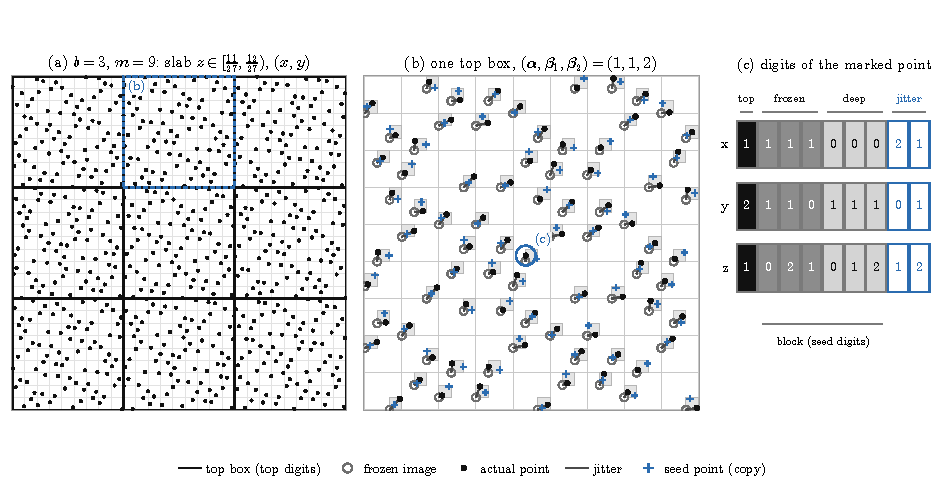
\includegraphics[width=\linewidth,height=0.5\textheight,keepaspectratio]{figs/base23_lift.pdf}}{\fbox{\parbox{0.9\textwidth}{\centering figure \texttt{base23\_lift} pending}}}
\caption{\baseTwoThreeCaption}
\label{fig:base23}
\end{figure}

The shifts in (1) are explicit, one per $m$: the shift of the seed, carried into the block digits by each lift. The definitions of \cite{DGS2} need only a family indexed by $m$, so the shifted nets are well-separated families of digitally shifted digital nets in their sense (Corollary~\ref{cor:dgs}). Part~(3) holds for every digital shift (Lemma~\ref{lem:shiftcert}). Its constants are those of (2) in base two and, for $m\equiv0,1$, lower in base three, where a shift can place a digit difference $0\cdots01\cdots1$ of two points on a carry chain. Digital $(0,m,3)$-nets in base $2$ were classified by Hofer and Suzuki \cite{HS19}; here we need only explicit seeds and the lift. Propagation rules for digital nets \cite[Sec.~4.2, 4.4]{DP10} control the quality parameter $t$, not distances; the lift is a propagation rule $m\to m+3$ at $t=0$ that also carries a separation certificate.

\begin{remark}[Why every-shift certificates vanish at some resolutions]\label{rem:shiftparity}
Along the chains the every-shift certificate $v^\circ_L$ vanishes at many resolutions (for $b=3$, $m\equiv0$, at every resolution below $18$; computed), and it is positive at the six certificate resolutions of Table~\ref{tab:base23}, all of them even. Two facts explain the pattern. (i) \emph{Parity.} If $L$ is even and $v^\circ_L=0$, then $v^\circ_{L+3}=0$ for every lift $P_{L+3}$ of $P_L$. Indeed, the indices $(n,0,0,0)$ of the lift (Definition~\ref{def:lift}) give points with top digit $0$, block digits those of $P_L$ and jitter digits $0$, so the top $\lfloor(L+3)/2\rfloor=H+1$ digits of their differences are $0$ followed by the top $H$ digits of the differences of $P_L$. For such differences the toroidal $\mu_{H+1}$ of the extended vector is at most the plain (non-toroidal) value of the original one, and a vector $\pm(0,\dots,0,1,\dots,1)$ has plain value $1$; so a vanishing certificate at $L$ gives one at $L+3$. For odd $L$ the window of $P_{L+3}$ gains one more block digit, so a certificate can first become positive only at an even resolution. (ii) \emph{Dichotomy.} If $v^\circ_L=0$, then along every lift chain from $P_L$ every $m\ge L$ in the class has $\min_\tau\delta(P_m\oplus\tau)N^{1/3}<2\sqrt3\,b^{\lceil L/2\rceil-2L/3}$. Indeed, the indices whose new digits are all $0$ embed $P_L$ into $P_m$ with top and jitter digits $0$, and a difference whose top window is $0$ or $\pm(0,\dots,0,1,\dots,1)$ in each coordinate can be shifted to have each coordinate below $2W$ in the units $b^{-(L+j)}$ of the proof of Lemma~\ref{lem:liftsep}, $m=L+3j$. So, for a chain frozen from every resolution, a floor $\kappa N^{-1/3}$, $\kappa>0$, that holds for every shift from some resolution on exists if and only if $v^\circ_L>0$ for some $L$; if the certificate vanished at infinitely many $L$, the every-shift separation would tend to $0$. For the nets of Theorem~\ref{thm:base23} the certificate is positive at every certificate resolution (Table~\ref{tab:base23}), so no shift makes their separation decay.
\end{remark}

The six seeds are printed in Table~\ref{tab:b23seeds} (Appendix~\ref{app:tables}); the chains, shifts and small-$m$ nets are data of the deposit, whose scripts rerun the certificates of Table~\ref{tab:base23} (Appendix~\ref{app:verify}).

\section{The question of Dick, Goda and Suzuki}\label{sec:dgs}
This section relates the results of Part~I to the definitions of \cite{DGS2}: low discrepancy, separation in their sense, digital shifts, and the maximum norm.

\begin{remark}[Low discrepancy]\label{rem:lowdisc}
All nets in this paper are $(0,m,s)$-nets in base $q$: every elementary box of volume $q^{-m}$ contains exactly one point (Lemma~\ref{lem:nie}). This is a property of the point set alone, whatever ring the net is digital over, so Niederreiter's discrepancy bound for $(t,m,s)$-nets in an integer base \cite{Nie87} applies: $D^*_N\le C_{s,q}(\log N)^{s-1}/N+O_{s,q}\bigl((\log N)^{s-2}/N\bigr)$ for $N=q^m$, with $C_{s,q}$ independent of $m$. So all our nets have low discrepancy in the sense of \cite{DGS2,DGLPS1}, and the question of Dick, Goda and Suzuki reduces, for these nets, to separation. The same holds for digitally shifted nets, which are again $(0,m,s)$-nets (Lemma~\ref{lem:shift}).
\end{remark}

\needspace{8\baselineskip}
\subsection{Digital shifts}
\begin{lemma}[Shifted graph forms]\label{lem:shift}
Let $P$ be a graph form over $\Z/q\Z$ with depths $\mathbf k$ and blocks $\Phi$, and $\tau=(\tau^{\mathrm{cell}}_c,\tau^{\mathrm{off}}_c)_c$ a digital shift (Definition~\ref{def:dshift}), split into its digits on the cell digits and on the offset digits of each coordinate. Then $P\oplus\tau$ is the set of points whose coordinate $c$ has the digits $n_c$ followed by $\sum_d\Phi_{cd}n_d+\gamma_c$, $n\in\prod_c(\Z/q\Z)^{k_c}$, where $\gamma_c=\tau^{\mathrm{off}}_c-\sum_d\Phi_{cd}\tau^{\mathrm{cell}}_d$. In particular $n$ is the cell of the point, every cell holds one point, $P\oplus\tau$ is a $(0,m,s)$-net if $P$ is, and for two points in the cells $n,n'$ every offset digit difference is congruent to the corresponding entry of $\Phi(n'-n)$ modulo $q$, as for $P$.
\end{lemma}

\begin{proof}
Substitute $n=\tilde n-\tau^{\mathrm{cell}}$ and index the shifted point by $\tilde n$. The shift maps every elementary box of shape $d$ bijectively onto one of the same shape, since it shifts the first $d_c$ digits of coordinate $c$.
\end{proof}

So a shifted net is an \emph{affine} graph form: offsets $\Phi n+\gamma$ with a constant $\gamma$. Lemma~\ref{lem:Ss}, Proposition~\ref{prop:Hk} and the skeleton lemmas of Section~\ref{sec:skel} hold for affine graph forms with the same proofs, since they use only differences of digits.

\begin{proposition}[Every digital shift]\label{prop:shift}
Lemma~\ref{lem:Ss} holds verbatim, with the same bound, for every digital shift of a graph form that satisfies (H1) and (H2). Consequently the lower bounds on the separation in Theorems~\ref{thm:A}, \ref{thm:main}, \ref{thm:S1}, \ref{thm:S2}, \ref{thm:allm} and \ref{thm:HL} and in Propositions~\ref{prop:D} and~\ref{prop:Hk} hold for every digital shift of the respective nets (in Theorem~\ref{thm:S1}(2) the occupied fine cells form a coset of the lattice), and so does the first-order sharpness in Theorem~\ref{thm:A}(2).
\end{proposition}

\begin{proof}
By Lemma~\ref{lem:shift} the shift only adds the constant $\gamma$ to the offsets. The proofs use the cells (the step and its carries), the residues of digit differences, the facts that a digit difference lies in $(-q,q)$ and vanishes if its residue does, and $|f'-f|<1$; the constant cancels in every residue, and in Lemma~\ref{lem:Ss} the deeper digits of a coordinate whose own axis alone moves are still equal, by (H2). Theorem~\ref{thm:S2} does not even need the re-indexing by the shifted cells: its proof uses only differences of the skeleton digits. The sharpness argument prescribes the cell digits and the first offset digits of a pair; in the shifted net these are digits of the unshifted net prescribed in translated sets of the same size, so the joint uniformity of the digits of the unshifted net, given by its $t=0$, suffices.
\end{proof}

The nets of Theorem~\ref{thm:base23}(1) carry one explicit shift by construction. Proposition~\ref{prop:shift} does not apply to them, because their bounds come from the lift certificates (Lemma~\ref{lem:liftsep}), not from Lemma~\ref{lem:Ss}; Theorem~\ref{thm:base23}(3) covers every digital shift instead. The per-prime nets of Remark~\ref{rem:perprime} keep their constants under every digital shift as well (Remark~\ref{rem:ppshift}). In dimension three, Proposition~\ref{prop:shift} gives every resolution under every digital shift:

\begin{corollary}[Corollary~\ref{cor:allm} under digital shifts]\label{cor:allmshift}
Let $p\ge37$ be prime. For every $m\ge3$ and every digital shift, the shifted nets of Corollary~\ref{cor:allm} satisfy its separation bounds, with the same constants $0.2715$ and $0.4250$, and its covering bounds; so they are quasi-uniform along every $N=p^m$, $m\ge3$, as the Larcher--Pillichshammer nets in \cite[Thm.~3.11]{DGS2}. For $m\ge4$ the lower bound still tends to $1$ as $p\to\infty$. At $m=3$ the nets are the column nets $\mathcal C_p$, whose three coordinates share the second and third digits, and the bound depends on whether the shift keeps them shared:
\begin{enumerate}
\item[(a)] for every shift, $\delta N^{1/3}>0.4693$;
\item[(b)] if the shift digits of the three coordinates agree at the second and at the third digit, the exact value of Theorem~\ref{thm:col}(2) holds;
\item[(c)] if they agree at the second digit, $\delta N^{1/3}\ge1-(7p-3)/(\sqrt3p^2)$;
\item[(d)] otherwise $1/\sqrt3-7/(\sqrt3p)\le\delta N^{1/3}\le1/\sqrt3+5/(\sqrt3p)$.
\end{enumerate}
\end{corollary}

\begin{proof}
A digital shift keeps one point in every cell and keeps $t=0$ (Lemma~\ref{lem:shift}), which is all the covering bounds use, except for the mesh-ratio constant $4.264$ of Corollary~\ref{cor:allm}, which comes from Theorem~\ref{thm:S1}(3); at $m=3$ this gives $h\le\sqrt3N^{-1/3}$. In the shifted net the occupied fine cells form a coset $g+\Lambda_A$ (Proposition~\ref{prop:shift}), and the proof of Theorem~\ref{thm:S1}(3) runs with its target residue moved by $g_z-\sum_d\rho^dg_{x_d}$; this is not a translation of the unshifted construction, since the target cell must stay in range. For $m\ge4$ the separation bounds of Theorems~\ref{thm:main}, \ref{thm:allm} and~\ref{thm:S1} used in Corollary~\ref{cor:allm} hold for every shift by Proposition~\ref{prop:shift}. For $m=3$ Proposition~\ref{prop:colshift} gives the lower bound $0.4693>0.4250$, the exact value and the bound for agreeing shift digits, and otherwise the two bounds $\frac1{\sqrt3}(1-\frac{W+3}p+\frac3{p^2})$ and $\frac1{\sqrt3}(1+\frac{3+w_{\max}}p-\frac3{p^2})$ with $W\le4$ and $w_{\max}\le2$, which lie in the stated interval.
\end{proof}

So only the limit changes, and only at $m=3$: with unequal shift digits at the geometric digit $\delta N^{1/3}$ lies within $7/(\sqrt3p)$ of $1/\sqrt3$. The reason: a digital shift adds a different constant to the shared digit in each coordinate, so the three coordinates no longer wrap at the same cells, and a step across a wrap of one coordinate alone has length about $1/\sqrt3$ (Remark~\ref{rem:glue}).

\begin{remark}[Shared digits under shifts]\label{rem:shiftshared}
So the exact value of Theorem~\ref{thm:col} does not extend to all shifted nets: if the shift digits of the three coordinates of $\mathcal C_q$ at the second digit are not all equal, then for every $q\ge11$, prime or not, the shifted net has $\delta N^{1/3}\le\frac1{\sqrt3}(1+\frac{3+w_{\max}}q-\frac3{q^2})$, below the value of Theorem~\ref{thm:col} (Proposition~\ref{prop:colshift}(3)). For each coordinate, the set of values of the shared digit at which a step wraps (its \emph{wrap window}) is translated by that coordinate's shift digit; unequal shift digits give distinct windows, so some cell wraps in exactly one coordinate, and its step along that axis gives the pair $qa_c\mathbf 1+\Delta j$ at integer scale. In general a digital shift translates the wrap windows independently in each coordinate. Bounds certified with arbitrary wraps (Remark~\ref{rem:glue}) therefore survive every shift; bounds that use locked wraps, wraps that are correlated across coordinates, need not. The nets $\mathcal T_p$ and $\mathcal W_p$ of Part~II are of the second kind (Remark~\ref{rem:wshift}).
\end{remark}

\subsection{Well-separated families}
In \cite{DGS2} a point set is \emph{$\kappa$-separated} ($\kappa$ as in \cite{DGS2}) if no (toroidal) shifted elementary interval with $\kappa$ digits in every coordinate contains two of its points \cite[Defs.~3.1--3.3]{DGS2}, and a family $(\mathcal P_m)_{m\in I}$ on an infinite set $I$ of resolutions is \emph{well separated} if $\mathcal P_m$ is $\kappa_m$-separated with $\kappa_m\le m/s+O(1)$ \cite[Def.~3.8]{DGS2} (in \cite{DGS2} the dimension is $d$).

\begin{corollary}[Well-separated families in the sense of Dick, Goda and Suzuki]\label{cor:dgs}
Let $s\ge2$ and $q\ge2$ be integers and $I\subseteq\N$ infinite, and for $m\in I$ let $\mathcal P_m\subset[0,1)^s$ be a $(0,m,s)$-net in base $q$ whose toroidal minimum distance satisfies $\delta\ge c\,q^{-m/s}$, with $c>0$ independent of $m$. Then every $\mathcal P_m$ is $\kappa_m$-separated and toroidally $\kappa_m$-separated in base $q$ \cite[Def.~3.3]{DGS2}, with
\[
\kappa_m=\Bigl\lceil\frac ms+\log_q\frac{\sqrt s}{c}\Bigr\rceil\ \le\ \frac ms+\log_q\frac{\sqrt s}{c}+1,
\]
so $(\mathcal P_m)_{m\in I}$ is a well-separated and toroidally well-separated family on $I$ \cite[Def.~3.8]{DGS2}. In particular:
\begin{enumerate}
\item the nets $\mathcal P_{k,q}$ of Theorem~\ref{thm:main}, for every integer $q\ge4$, are $(k+1)$-separated, i.e.\ $\kappa_m=m/3+1$ on $I=\{3k:k\ge2\}$;
\item the nets of Theorem~\ref{thm:A}(2) are $(k+1)$-separated on $I=\{sk:k\ge1\}$;
\item the nets $\mathcal H^s_{k,p}$ of Theorem~\ref{thm:HL} are $(k+1)$-separated for every prime $p\ge\max(2s,2B_s+4)$ (two more than in Theorem~\ref{thm:HL}; see Step~3 of the proof) and every $k\ge1$;
\item the nets $\mathcal S^1_{k,p,\rho}$ of Theorem~\ref{thm:S1}, with $m=sk+s-1$, are $(k+1)$-separated, i.e.\ $\kappa_m=\lceil m/s\rceil$, if $(\rho-1)^2\ge s$ (for $\rho=\lfloor p^{1/s}\rfloor$ this holds when $p>(\lceil\sqrt s\rceil+1)^s$), and $(k+2)$-separated otherwise;
\item for every prime $p\ge37$ the nets of Corollary~\ref{cor:allm} are $(\lfloor m/3\rfloor+1)$-separated for every $m\ge3$.
\end{enumerate}
All of these hold toroidally as well, and for every digital shift (Definition~\ref{def:dshift}) of the respective nets. For prime $q$ the nets are digital nets over $\F_q$ in the sense of \cite[Def.~2.1]{DGS2}; this covers (3)--(5) entirely and the prime instances of (1) and~(2). For composite $q$ the nets of (1) and (2) are digital over $\Z/q\Z$, which is not covered by \cite[Def.~2.1]{DGS2}; Definitions~3.1 and~3.2 of \cite{DGS2} are stated for every integer base $b\ge2$, and we read Definitions~3.3 and~3.8 in the same generality.
\end{corollary}

\begin{proof}
\emph{Step 1 (\cite[Lemma~3.7]{DGS2}, with strict inequality).} Let $P\subset[0,1)^s$ be finite and $\kappa\ge0$, and suppose every two distinct points of $P$ have toroidal $\ell^\infty$-distance at least $q^{-\kappa}$. A toroidal shifted elementary interval $\tilde J_{\mathbf c,a,e}$ with $\kappa$ digits in every coordinate, $\mathbf c=(\kappa,\dots,\kappa)$ \cite[Def.~3.2]{DGS2}, is contained in a product of sets $I_j\bmod1$, where $I_j=[\alpha_j,\alpha_j+q^{-\kappa})$ is half-open. If $x,y\in\tilde J_{\mathbf c,a,e}$, then for each $j$ there are $z,z'\in\Z$ with $x_j+z,\ y_j+z'\in I_j$, so $\min(|x_j-y_j|,1-|x_j-y_j|)\le|(x_j+z)-(y_j+z')|<q^{-\kappa}$, and hence $x=y$. So $P$ is toroidally $\kappa$-separated. A non-toroidal interval $J_{\mathbf c,a,e}$ gives the same bound for $|x_j-y_j|$, which is at least the toroidal distance, so $P$ is also $\kappa$-separated. This sharpens the contrapositive of \cite[Lemma~3.7]{DGS2} to the strict bound $q_\infty(P)<1/(2q^\kappa)$ for non-separated $P$, where $q_\infty(P)$ is the separation radius of \cite{DGS2} in the maximum norm; the strictness comes from the intervals being half-open.

\emph{Step 2.} For distinct $x,y\in\mathcal P_m$ the toroidal coordinate distances $t_j$ satisfy $\sum_jt_j^2\ge\delta^2$, so $\max_jt_j\ge\delta/\sqrt s\ge(c/\sqrt s)\,q^{-m/s}\ge q^{-\kappa_m}$ by the choice of $\kappa_m$. Since toroidal distances are at most $\sqrt s/2$, we have $c\,q^{-m/s}\le\sqrt s/2$, so $\kappa_m\ge1$. Step~1 gives the separation, and $\kappa_m-m/s\le1+\log_q(\sqrt s/c)$ is bounded, which is the condition of \cite[Def.~3.8]{DGS2}.

\emph{Step 3 (the families).} By Step~2 a net with $\delta\ge\theta\,q^{-\kappa}$ is $\kappa$-separated as soon as $\theta\ge\sqrt s$.
(1) $m=3k$ and $\delta\ge c(q)q^{-k}$ (Theorem~\ref{thm:sep}); with $\kappa=k+1$ we need $q\,c(q)\ge\sqrt3$, i.e.\ $\min\{(q-1)^2,(q-2)^2+(q-4)^2,3(q-3)^2\}\ge3$, which holds for $q\ge4$ (with equality at $q=4$).
(2) $\delta\ge(1-a^*_s/q)q^{-k}$; with $\kappa=k+1$ we need $q-a^*_s\ge\sqrt s$. From $q\ge5a^*_s+4$ we get $q-a^*_s\ge\frac45(q+1)$, and from $\operatorname{lpf}(q)\ge s-1$ we get $q+1\ge s$, so $q-a^*_s\ge\frac45s\ge\sqrt s$ for $s\ge2$.
(3) $\delta\ge c_p\,p^{-k}$ with $c_p=\min(\sqrt s(\frac12-\epsilon_p),\sqrt2(1-\epsilon_p))$ and $\epsilon_p=(B_s+1)/p$; with $\kappa=k+1$ we need $p\,c_p\ge\sqrt s$. If $p\ge2B_s+4$, then $\sqrt s(\frac12-\epsilon_p)p=\frac{\sqrt s}2(p-2B_s-2)\ge\sqrt s$ and $\sqrt2(1-\epsilon_p)p\ge p/\sqrt2\ge\sqrt2\,s\ge\sqrt s$, since $\epsilon_p\le\frac12$ and $p\ge2s$.
(4) $m=sk+s-1$ and $\delta\ge(\rho-1)p^{-(k+1)}$ (Theorem~\ref{thm:S1}(1)); $\kappa=k+1$ needs $\rho-1\ge\sqrt s$, and otherwise $\kappa=k+2$ needs $(\rho-1)p\ge\sqrt s$, which holds as $p>2^s$. If $p>(\lceil\sqrt s\rceil+1)^s$, then $\rho=\lfloor p^{1/s}\rfloor\ge\lceil\sqrt s\rceil+1$.
(5) $m=3$: $\delta\ge\sqrt{2/3}\,p^{-1}$ (Theorem~\ref{thm:colmin}), and $\kappa=2$ needs $p\sqrt{2/3}\ge\sqrt3$, i.e.\ $p\ge3/\sqrt2$. $m=3k$, $k\ge2$: part~(1). $m=3k+1$: $\delta\ge(\rho^2-4)p^{-(k+1)}$ with $\rho$ maximal subject to $\rho^2(\rho+1)\le p$ (Theorem~\ref{thm:allm}), and $p\ge37$ gives $\rho\ge3$, so $\rho^2-4\ge5\ge\sqrt3$ and $\kappa=k+1$. $m=3k+2$: part~(4) with $s=3$ and $\rho=\lfloor p^{1/3}\rfloor\ge3$, so $(\rho-1)^2=4\ge3$ and $\kappa=k+1$. In every case $\kappa_m=\lfloor m/3\rfloor+1$.

\emph{Digital shifts.} By Proposition~\ref{prop:shift} the separation bounds used in (1)--(4) and, for $m\ge4$, in (5) hold for every digitally shifted net. For $m=3$, Proposition~\ref{prop:colshift}(3) gives $\delta\ge\frac1{\sqrt3}(1-\frac{W+3}p+\frac3{p^2})\,p^{-1}$ with $W\le4$, and $\kappa=2$ needs $p^2-(W+6)p+3\ge0$, which holds for $p\ge10$.
\end{proof}

The nets of Theorem~\ref{thm:base23}, with their shifts, are digitally shifted digital nets over $\F_b$, $b\in\{2,3\}$, in the sense of \cite[Def.~2.2]{DGS2}, so the corollary applies to them as well, with $\kappa_m=\lceil m/3+\log_b(\sqrt3/c)\rceil$: for every digital shift with the constants $c$ of part~(3), and with the larger constants of part~(1) for its explicit shifts. Likewise the per-prime nets of Remark~\ref{rem:perprime}, with the constants of Table~\ref{tab:perprime}, are well separated under every digital shift (Remark~\ref{rem:ppshift}).

\begin{remark}[Finitely many resolutions]\label{rem:dgsfinite}
Definition~3.8 of \cite{DGS2} constrains only $m\in I$, and finitely many further resolutions can be added at no cost. If $\mathcal Q\subset q^{-m}\Z^s\cap[0,1)^s$ is a $(0,m,s)$-net in base $q$, the elementary boxes of shape $(m,0,\dots,0)$ each hold one point, so the first coordinates of the points are distinct elements of $q^{-m}\Z\cap[0,1)$ and any two of them have toroidal distance at least $q^{-m}$; by Step~1 of the proof of Corollary~\ref{cor:dgs}, $\mathcal Q$ is $m$-separated and toroidally $m$-separated. Adding finitely many such $m$ to $I$ changes the $O(1)$ of \cite[Def.~3.8]{DGS2} by a constant. In dimension three digital $(0,m,3)$-nets over $\Z/q\Z$ exist for every integer $q\ge2$ (over $\F_p$ for every prime $p$) and every $m\ge1$: by Lemma~\ref{lem:Ts}, whose proof does not use $m\equiv0\pmod s$, every box minor of the frame of the places $\infty,0,1$ is $\pm1$, a unit modulo every $q$, so the frame is one (Lemma~\ref{lem:nie}; see also \cite[Thm.~6.2, Cor.~6.3]{Nie87} and \cite[Sec.~8.2]{DP10}), and trivially for $m=0$. Together, Theorems~\ref{thm:main} and~\ref{thm:col}, Corollary~\ref{cor:allm}, Remark~\ref{rem:perprime} and Theorem~\ref{thm:base23} cover all but finitely many $m$ in each prime base with a constant independent of $m$; with the frame nets for the remaining $m$ they give well-separated families on all of~$\N$, in every prime base. The same holds under every digital shift: the constants survive every shift (Proposition~\ref{prop:shift}, Corollary~\ref{cor:allmshift}, Remark~\ref{rem:ppshift} and Theorem~\ref{thm:base23}(3)), and a digitally shifted $(0,m,s)$-net is again a $(0,m,s)$-net on the grid $q^{-m}\Z^s$ (Lemma~\ref{lem:shift}), so the argument above applies to it.
\end{remark}

\subsection{The maximum norm}
\cite{DGS2} measure separation and mesh ratios also in the maximum norm. Since $\Vert x\Vert_\infty\ge\Vert x\Vert_2/\sqrt3$, the Euclidean bound gives $\delta_\infty\ge(1-1/q)q^{-k}/\sqrt3$ for the nets of Theorem~\ref{thm:main}; the sign analysis in the proof of Theorem~\ref{thm:sep} gives more:

\begin{proposition}[Maximum norm]\label{prop:linf}
Let $q\ge4$, $k\ge2$. For every digital shift $\tau$, any two distinct points of $\mathcal P_{k,q}\oplus\tau$ have toroidal $\ell^\infty$-distance at least $(1-3/q)\,q^{-k}$. Hence the $\ell^\infty$ mesh ratio of $\mathcal P_{k,q}\oplus\tau$ in the sense of \cite{DGS2}, toroidal or not, is at most $2q/(q-3)$, and $\mathcal P_{k,q}\oplus\tau$ is toroidally $(k+1)$-separated \cite[Def.~3.3]{DGS2}.
\end{proposition}

\begin{proof}
By Proposition~\ref{prop:shift} the proof of Theorem~\ref{thm:sep} applies to $\mathcal P_{k,q}\oplus\tau$. In its sign analysis every step has a coordinate with $|\Delta_i|\ge1-3/q$ ($=\beta_3$ in that proof): an own-axis step has $\beta_1$; for $\nu=2$, (iv) gives a backward coordinate with $|\sigma|\le1$ or $\sigma=0$; for $\nu=3$, a forward coordinate or a backward one with $|\sigma|=3$ forces a backward one with $|\sigma|\le1$ by (ii), (iii), and otherwise all three are backward with $|\sigma|\le2$. One point per cell gives $h_\infty\le q^{-k}$, and $(1-3/q)q^{-k}\ge q^{-k-1}$ for $q\ge4$; the separation statement is Step~1 of the proof of Corollary~\ref{cor:dgs}.
\end{proof}

The constant $3$ is the exact $\ell^\infty$ value of the relaxation of Lemma~\ref{lem:Ss} for this geometric layer, attained at the step $e=\mathbf 1$ with three carries. For a dominant design (Proposition~\ref{prop:D}) every moving coordinate is backward with $|\sigma_i|\le2a$, so the same argument gives $\delta_\infty\ge(1-(2a+1)/q)\,q^{-k}$ and an $\ell^\infty$ mesh ratio at most $2q/(q-2a-1)$ for every $q\ge2a+2$ and every digital shift, in particular below $10/3$ for the nets of Theorem~\ref{thm:A}(2).

\emph{The sequence question.} All nets here depend on $m$; they are not prefixes of one sequence, and the question of \cite{DGS2} for sequences (a sequence whose first $q^m$ points are well separated for every $m$, \cite[Def.~3.8]{DGS2}) remains open in dimension $s\ge3$ (Remark~\ref{rem:open}(10)).

\part{Separation constants}\label{part:constants}
Part~I proves bounds $\delta N^{1/s}\ge c$ with explicit constants $c$. Part~II asks how large $c$ can be. At the resolutions $m=sk$ the bounds of Part~I have the form $1-K/q$, and for a family of nets with $\delta N^{1/s}=1-K/q+O(q^{-2})$ as $q\to\infty$ we call $K$ its \emph{first-order deficit}, or simply its deficit. Sections~\ref{sec:deficit} and~\ref{sec:deficitgrowth} bound the deficit from above for given designs and from below for whole classes of nets. Section~\ref{sec:drift} explains the deficits $\frac13$ and $\frac23$ of the column nets, whose geometric layers have entries of size about $q/3$. Section~\ref{sec:whylat} shows why the cubic value $1$, the value of $\Z^s$ with one point per cell, is a natural barrier when the cells are cubes, and Section~\ref{sec:large} goes beyond it.

\section{The first-order deficit: certificates and ceilings}\label{sec:deficit}
This section works with designs. Its first subsection turns the one-digit relaxation into a number, the \emph{certified deficit} $K(F)$ of a design $F$, and shows how a finite computation (a \emph{certificate}) proves the bound $1-K(F)/q$ at every admissible base (defined after Proposition~\ref{prop:Dprime}). The second subsection proves \emph{ceilings}: upper bounds on $\delta N^{1/s}$ that hold for a whole class of nets. The remaining subsections give the designs with the smallest certified deficits that we have, in dimension four and at $k=1$. Section~\ref{sec:deficitgrowth} shows why the deficit must grow with $s$.

\subsection{The certified deficit of a design}
Remark~\ref{rem:K} expands the relaxation $\mathrm{LB}$ of Lemma~\ref{lem:Ss} for a fixed design as $1-K/q+O(q^{-2})$; we now define this $K$ precisely. Let $F=(F_0,\dots,F_{L-1})$ be a design with integer partial sums $M^{(j)}$. A \emph{configuration} $(e,j)$ is a step $e\in\{-1,0,1\}^s\setminus\{0\}$ with carry depths $j_d\in\{0,\dots,L-1\}$ on its moving axes, with $\sigma_i=\sum_de_dM^{(j_d)}[i][d]$ and $\mathrm{jit}_i$ as in Lemma~\ref{lem:Ss}. A moving coordinate is backward or forward as in Remark~\ref{rem:K}: a \emph{backward} coordinate ($e_i\sigma_i\le0$) has its geometric digit move against the step, so its point lands about one cell away; a \emph{forward} one has it move with the step, so its point may land almost on that of its neighbour.

\begin{definition}[Certified first-order deficit]\label{def:K}
The \emph{cost} of a configuration is $|\sigma_b|+\mathrm{jit}_b$ if exactly one moving coordinate $b$ is backward, $0$ if at least two are, and $+\infty$ if none is. The \emph{certified deficit} $K(F)$ is the maximum of the cost over all configurations, and $\sigma_{\max}(F)$ is the maximum of $|\sigma_i|$ over all configurations and all $i$.
\end{definition}

The cost counts, in units of $1/q$ of a cell, by how much the step falls short of a full cell at first order. A one-axis step along $a$ with carry depth $j$ has cost $\alpha^{(j)}_a=-M^{(j)}[a][a]$ if this is $\ge0$, and $+\infty$ otherwise. For a dominant design (Proposition~\ref{prop:D}) every moving coordinate is backward, so $K(F)=\max_c\alpha_c$, the number $a$ of Proposition~\ref{prop:D}. Both $K(F)$ and $\sigma_{\max}(F)$ are maxima over the $(2L+1)^s-1$ configurations, and $\sigma_{\max}(F)=\max_i\sum_d\max_j|M^{(j)}[i][d]|$. The certified deficit is an upper bound for the deficit of every family of nets that realizes $F$ (Proposition~\ref{prop:Dprime}); it need not equal it.

\begin{proposition}[Certificate for all large $q$]\label{prop:Dprime}
Let $F$ be a design with $K=K(F)<\infty$ and $\sigma_{\max}=\sigma_{\max}(F)$, and put
\[
q_{\mathrm{tail}}(K,\sigma_{\max})=\max\Bigl(\sigma_{\max}+1,\ \Bigl\lceil\frac{\sqrt2(\sigma_{\max}+1)-K}{\sqrt2-1}\Bigr\rceil\Bigr).
\]
Then $\mathrm{LB}\ge1-K/q$ for every $q\ge q_{\mathrm{tail}}(K,\sigma_{\max})$, where $\mathrm{LB}$ is the relaxation of Lemma~\ref{lem:Ss} for $F$ or for any truncation $(F_0,\dots,F_{L'-1})$, $L'\le L$.
\end{proposition}

\begin{proof}
Fix a configuration and let $q\ge q_{\mathrm{tail}}$, so $q>\sigma_{\max}\ge|\sigma_i|$ for all $i$. For a moving backward coordinate $i$ the bound $b_i$ of Lemma~\ref{lem:Ss} is $q-|\sigma_i|-\mathrm{jit}_i\ge0$: for $e_i=1$ and $-q<\sigma_i<0$, $\bar\sigma_i=q+\sigma_i$ and the two options give $|q+t|\in\{2q-|\sigma_i|,\,q-|\sigma_i|\}$; for $\sigma_i=0$ the only option gives $q$; $e_i=-1$ is symmetric. If at least two coordinates are backward, $\sum_ib_i^2\ge2(q-\sigma_{\max}-1)^2\ge(q-K)^2$, because $\sqrt2(q-\sigma_{\max}-1)\ge q-K$ is the second condition on $q_{\mathrm{tail}}$ (and $K\le\sigma_{\max}+1\le q$). If exactly one coordinate $b$ is backward, $\sum_ib_i^2\ge(q-|\sigma_b|-\mathrm{jit}_b)^2\ge(q-K)^2$. No backward coordinate is excluded by $K<\infty$. So every configuration gives $(\sum_ib_i^2)^{1/2}/q\ge1-K/q$. The configurations of a truncation are among those of $F$, with the same $\sigma$ (Lemma~\ref{lem:Ss}, capped carry depths), so its $\mathrm{LB}$ is at least that of $F$.
\end{proof}

For a dominant design $K=a$ and $\sigma_{\max}\le2a$, and $q_{\mathrm{tail}}\le\lceil((2\sqrt2-1)a+\sqrt2)/(\sqrt2-1)\rceil<5a+4$ for $a\ge1$: Proposition~\ref{prop:Dprime} is the proof of Proposition~\ref{prop:D} without the dominance hypothesis. It turns every statement ``$\mathrm{LB}\ge x$ for every admissible $q\ge q_0$'' about a fixed design into a finite computation (a certificate): $K(F)$ and $\sigma_{\max}(F)$, and the exact value of $\mathrm{LB}$ at the finitely many admissible $q<\max(q_{\mathrm{tail}},K/(1-x))$. Here the \emph{admissible} bases of a design are those for which Corollary~\ref{cor:tsk} gives a net, $\gcd(q,DD')=1$ (Definition~\ref{def:Ns}); on the places $\infty,0,1,\dots,s-2$ they satisfy $\operatorname{lpf}(q)\ge s-1$. This is how the thresholds below are certified.

The relaxation never certifies a deficit below $1$:

\begin{lemma}[The relaxation stops at one]\label{lem:Kone}
Let $F$ be a design with some nonzero off-diagonal entry $F_0[a][b]$. Then $K(F)\ge1$.
\end{lemma}

\begin{proof}
Write $M=F_0$ and consider the carry-free steps $e=\e_a+\varepsilon\e_b$, $\varepsilon=\pm1$, along which only $a$ and $b$ move, with $\sigma_a=M_{aa}+\varepsilon M_{ab}$ and $\varepsilon\sigma_b=M_{bb}+\varepsilon M_{ba}$. If for some $\varepsilon$ at most one of $a$, $b$ is backward, that configuration costs at least $\mathrm{jit}=1$, or $+\infty$. Otherwise $M_{aa}+\varepsilon M_{ab}\le0$ for both signs, so $M_{aa}\le-|M_{ab}|\le-1$, and the one-axis step along $a$ without carry costs $-M_{aa}\ge1$.
\end{proof}

By Lemma~\ref{lem:phase}(ii) (Section~\ref{sec:whylat}) the off-diagonal entries of the geometric layer of a digital $(0,sk,s)$-net are units modulo $q$, hence nonzero. So for every design with $|F_0|<q/2$, whose geometric layer is $F_0$, the bounds of Lemma~\ref{lem:Ss} and Proposition~\ref{prop:Dprime} certify at most $1-1/q$ at first order. This concerns what the relaxation certifies, not the true distance; ceilings for the true distance are Corollary~\ref{cor:ceil3} and the results of Section~\ref{sec:deficitgrowth}. Deficits below $1$ need layers whose entries grow with $q$; for the column nets of Section~\ref{sec:m3} the minimum distance is determined in closed form instead (Theorem~\ref{thm:col}, Section~\ref{sec:drift}).

\subsection{The first-order ceiling}\label{sec:ceil}
The idea of the ceiling: a step to the neighbouring cell along an axis $a$ moves coordinate $a$ by about $1+\tilde M_{aa}/p$ cells and every other coordinate $u$ by about $\tilde M_{ua}/p$, unless a digit wraps; the $t=0$ property lets us count cells and find one where the digits behave as required.

\begin{proposition}\label{prop:ceil}
Let $p$ be an odd prime, $k\ge2$, and let $\mathcal P$ be a digital $(0,3k,3)$-net over $\F_p$ with normalized minimum distance $c=\delta N^{1/3}$ (toroidal or not). Let $a$, $b$, $b'$ be the three coordinates $x$, $y$, $z$ in some order.
\begin{enumerate}
\item[(i)] If $\tilde M_{aa}\le-1$, then $c^2<(1-1/p+p^{1-k})^2+\bigl((|\tilde M_{ba}|+1)^2+(|\tilde M_{b'a}|+1)^2\bigr)/p^2$.
\item[(ii)] If $\tilde M_{aa}\ge1$, then $c^2<\bigl((\tilde M_{aa}+1)^2+(|\tilde M_{ba}|+1)^2+(|\tilde M_{b'a}|+1)^2\bigr)/p^2$.
\end{enumerate}
\end{proposition}

\begin{proof}
Let $\mu\in\{1,\dots,p-1\}$ be the least nonnegative residue of $(\Phi_{aa})_{0,k-1}$, so $\mu=p+\tilde M_{aa}$ in (i) and $\mu=\tilde M_{aa}$ in (ii). Take a cell $n$ with $n_a=0$ and its neighbour $n+e_a$; only the last digit of $n_a$ changes, so each offset digit of each coordinate changes by a constant modulo $p$, the first one of coordinate $u$ by $(\Phi_{ua})_{0,k-1}$. Require
(A) the first $k-1$ offset digits of $a$ all equal $p-1$, and
(B) for $u\in\{b,b'\}$, the first offset digit of $u$ is not in the set $W_u$ of the $|\tilde M_{ua}|$ digit values on which adding $\tilde M_{ua}$ leaves $\{0,\dots,p-1\}$.
Under (A) the first offset digit of $a$ becomes $\mu-1$, the next $k-2$ (all $p-1$) can only decrease, and the remaining digits contribute less than $p^{1-k}$. So in cell units $\Delta_a=\mu/p+\theta$ with $-1/p<\theta<p^{1-k}$. Under (B), the first offset digit of $u$ changes by exactly $\tilde M_{ua}$, so $|\Delta_u|<(|\tilde M_{ua}|+1)/p$. In (i), $0<\Delta_a<1-1/p+p^{1-k}$; in (ii), $0<\Delta_a<\tilde M_{aa}/p+p^{1-k}\le(\tilde M_{aa}+1)/p$ since $k\ge2$.
It remains to find such a cell. The $p^{2k}$ indices with $n_a=0$ are parametrized by $(n_b,n_{b'})$. By the $t=0$ boxes $(2k-1,k+1,0)$ and $(2k-1,0,k+1)$ (order $a,b,b'$), exactly $p^{k+1}$ of them satisfy (A), and among these the first offset digits of $b$ and of $b'$ each take every value exactly $p^k$ times. Hence at most $(|W_b|+|W_{b'}|)p^k\le(p-1)p^k<p^{k+1}$ of them violate (B), since $|\tilde M_{ua}|\le(p-1)/2$. The pair $n$, $n+e_a$ lies inside the cube, so it bounds the toroidal and the Euclidean distance.
\end{proof}

\begin{corollary}[First-order ceiling in dimension three]\label{cor:ceil3}\label{prop:A}% rev 15.7: was the unnumbered ``Proposition A''; prop:A kept as an alias
Let $p$ be an odd prime and $k\ge2$. Suppose the first offset digit of some coordinate $a$ of a digital $(0,3k,3)$-net over $\F_p$ depends on the last cell digit of $a$ with a coefficient whose centred representative is nonzero, and the coefficients of the other two coordinates on that digit are bounded by $C\ge1$ in absolute value. If that representative is $\le-1$ and $k\ge3$, then $\delta N^{1/3}<1-1/p+7C^2/p^2$. If it lies in $[1,C]$, then $\delta N^{1/3}<4C/p$.
\end{corollary}

\begin{proof}
The coefficient of the corollary is $\tilde M_{aa}$; let $|\tilde M_{ba}|,|\tilde M_{b'a}|\le C$, $C\ge1$. In (i) of Proposition~\ref{prop:ceil}, with $k\ge3$, put $\alpha=1-1/p+p^{1-k}\ge2/3$ and $\beta=\bigl((|\tilde M_{ba}|+1)^2+(|\tilde M_{b'a}|+1)^2\bigr)/p^2\le8C^2/p^2$; then $c<\sqrt{\alpha^2+\beta}\le\alpha+\beta/(2\alpha)\le\alpha+6C^2/p^2$, and $p^{1-k}\le1/p^2\le C^2/p^2$, so $c<1-1/p+7C^2/p^2$. In (ii), with $1\le\tilde M_{aa}\le C$, $c^2<3(C+1)^2/p^2\le12C^2/p^2$, so $c<4C/p$. (For $k=2$ the term $p^{1-k}=1/p$ cancels the $-1/p$; hence $k\ge3$.)
\end{proof}

For $\mathcal P_{k,p}$ ($\tilde M=M$), Proposition~\ref{prop:ceil}(i) gives $c^2<(1-1/p+p^{1-k})^2+8/p^2$, i.e. $c<1-1/p+4/p^2+O(p^{-3})$ for $k\ge4$ ($5/p^2$ for $k=3$). So the lower bound $c(p)=1-1/p$ of Theorem~\ref{thm:main} is sharp to first order for $p\ge11$. For $\tilde M_{aa}=0$ the same counting (now with $0<\Delta_a<1+1/p$) only gives $c^2<(1+1/p)^2+\bigl((|\tilde M_{ba}|+1)^2+(|\tilde M_{b'a}|+1)^2\bigr)/p^2$.

\begin{corollary}[Ceiling in every dimension]\label{cor:ceils}
Let $s\ge3$, $k\ge2$, and let $\mathcal P$ be a digital $(0,sk,s)$-net over $\Z/q\Z$, $q\ge3$, in graph form, with geometric layer $\tilde M$ and $c=\delta N^{1/s}$ (toroidal or not). Let $a$ be a coordinate with $\sum_{u\ne a}|\tilde M_{ua}|<q$.
\begin{enumerate}
\item[(i)] If $\tilde M_{aa}\le-1$, then
\[
c^2<\Bigl(1-\frac{|\tilde M_{aa}|}q+q^{1-k}\Bigr)^2+\sum_{u\ne a}\frac{(|\tilde M_{ua}|+1)^2}{q^2}.
\]
\item[(ii)] If $\tilde M_{aa}\ge1$, then
\[
c^2<\frac{(\tilde M_{aa}+1)^2+\sum_{u\ne a}(|\tilde M_{ua}|+1)^2}{q^2};
\]
in particular $c<\sqrt s\,(C+1)/q$ if $|\tilde M|\le C$.
\end{enumerate}
\end{corollary}

\begin{proof}
The proof of Proposition~\ref{prop:ceil} applies with all counts multiplied by $q^{(s-3)k}$ and $\Delta_a=\mu/q+\theta$, $\mu=q+\tilde M_{aa}$ in (i), $\mu=\tilde M_{aa}$ in (ii) (where $0<\Delta_a<(\tilde M_{aa}+1)/q$ as $k\ge2$). The boxes used have depth $0$ off $a$ and the transverse coordinate considered, and total depth $\le3k\le sk$; no field structure is used; and the union bound over $u\ne a$ leaves a cell because $\sum_{u\ne a}|\tilde M_{ua}|<q$.
\end{proof}

So for a design whose certified deficit is attained by a one-axis step, $K(F)=-F_0[a][a]$, Proposition~\ref{prop:Dprime} and Corollary~\ref{cor:ceils}(i) together give $\delta N^{1/s}=1-K(F)/q+O(q^{-2})$ for $k\ge3$, and for $k\ge2$ when the deeper rows of the diagonal blocks vanish ((H2) of Lemma~\ref{lem:Ss}), which removes the term $q^{1-k}$; this is the sharpness argument in the proof of Theorem~A.

\begin{remark}[The sign of the diagonal; diagonal zero]\label{rem:sign}\label{rem:diag0}
Case (i) of the sign analysis in the proof of Theorem~\ref{thm:sep} uses the diagonal entry $-1$ of $M$: on a step along its own axis a coordinate moves by $1-1/q$ cells, slightly less than a full cell, never slightly more. Replacing it by $+1$ (in $\mathcal P_{k,q}$: row $k$ of $E$ becomes $(Ed)_k=-d_{k-1}+d_k$, which changes only the entry $(\Phi_{cc})_{0,k-1}$) keeps $t=0$ (Lemma~\ref{lem:gauge}(a)), but for odd prime $q$ Proposition~\ref{prop:ceil}(ii) caps the minimum distance at $O(1/q)$. If $\tilde M_{aa}=0$ for all $a$, Proposition~\ref{prop:ceil} does not apply; heuristically such layers stay below $1-1/p$ at first order too, but the argument would need a joint condition on three digits that is not a single box, and we have no proof (Remark~\ref{rem:open}(1)).
\end{remark}

\subsection{Designs with small deficit}\label{sec:Kdesigns}
The design $U^*_s$ of Theorem~A is fixed by a rule (for each column and carry depth, a short admissible design column reduced against the earlier ones, Definition~\ref{def:Ustar}) and is not optimized for $K$. A local search over admissible design columns (Lemma~\ref{lem:sat}) and over diagonals, with $K(F)$ evaluated exactly, gives the designs of Table~\ref{tab:Kdesigns}. Its row scalars are fixed in advance: $\lambda'\equiv1$ for $s=4$, and for $s\ge5$ the values $\lambda'_\infty=\frac12$, all other $\lambda'_c=1$, a choice taken over from an earlier search over row scalars for designs with small entries; the other row scalars we tried did not give a smaller $K(F)$. Each column of the partial sums $M^{(j)}$ is taken from a precomputed pool of short admissible columns; a move replaces the column of one pair (column, carry depth) by another from the pool, flips its sign, or changes a diagonal entry by $\pm1$, and a move is kept if it lowers $K(F)$, or keeps $K(F)$ without raising the number of configurations that attain it; the search stops after a fixed running time. The search program is not part of the software deposit. The search only proposes designs; every entry of the table is certified for the design found, independently of how it was found. Each is reachable (Proposition~\ref{prop:F}, checked by exact interpolation), so by Corollary~\ref{cor:tsk} it gives digital $(0,sk,s)$-nets for every admissible $q$ and every $k\ge1$; by Proposition~\ref{prop:Dprime} and an exact scan of the smaller admissible $q$ their relaxations certify the thresholds of the table for every $k\ge1$.

\begin{table}[tbp]
\centering\small\setlength{\tabcolsep}{4.5pt}
\begin{tabular}{@{}lccccc@{}}
\toprule
$s$ & 4 & 5 & 6 & 7 & 8\\
\midrule
certified deficit $K(F)$ & 2 & 5 & 10 & 33 & 127\\
$\sigma_{\max}(F)$; largest $|M^{(j)}|$ & 7; 2 & 21; 8 & 63; 22 & 194; 104 & 754; 254\\
ring $R'$ & $\Z[\frac12]$ & $\Z[\frac16]$ & $\Z[\frac16]$ & $\Z[\frac1{30}]$ & $\Z[\frac1{30}]$\\
$q_{\mathrm{tail}}$ (Prop.~\ref{prop:Dprime}) & 23 & 64 & 195 & 587 & 2272\\
$\mathrm{LB}\ge1-K/q$ for $q\ge$ & 17 & 31 & 61 & 197 & 461\\
$\mathrm{LB}\ge.5/.8/.9$ for $q\ge$ & 11/15/21 & 23/29/53 & 41/59/91 & 107/187/323 & 331/631/1261\\
\midrule
$a^*_s$ (Table~\ref{tab:astar}) & 5 & 16 & 43 & 170 & 543\\
lower bound on $K(F)$ (Prop.~\ref{prop:E}) & 1 & 2 & 6 & 12 & 60\\
status & c.-a. & c.-a. & c.-a. & computed & computed\\
\bottomrule
\end{tabular}
\medskip
\caption{Searched designs on the places $\infty,0,1,\dots,s-2$ (data: Appendix~\ref{app:designs} for $s\le6$; all in the deposit). The thresholds hold for every admissible $q$ from the value shown and every $k\ge1$ (least such admissible values; admissible means $\operatorname{lpf}(q)\ge s-1$: odd $q$ for $s=4$, $\gcd(q,6)=1$ for $s=5,6$, $\gcd(q,30)=1$ for $s=7,8$). \emph{c.-a.}: computer-assisted, by full enumeration of the $(2L+1)^s-1=(2s-1)^s-1$ configurations ($L=s-1$), the exact relaxation at every admissible $q$ below the tail, and Proposition~\ref{prop:Dprime} beyond it, reproduced by an independent implementation. For $s=7,8$ the same computations were run and reproduced, but we state these rows as computed values only: their designs are not printed here, and the deposit scripts do not rerun these enumerations. The searched $K$ are upper bounds for the best certified deficit of a design on these places, not optimal values. The lower bound $\operatorname{lcm}(1,\dots,s-3)$ applies to every design whose row scalars are constant on the finite places, these included.}
\label{tab:Kdesigns}
\end{table}

\subsection{Dimension four}\label{sec:dim4ex}
We work out the smallest case beyond dimension three: a design with certified deficit two, which is also the true deficit of its nets. Remark~\ref{rem:pm1} below explains why its entries have size two. For $s=4$ and the places $\infty,0,1,2$ the place differences are $\pm1,\pm2$, so $R=\Z[\frac12]$. In the normal form (Propositions~\ref{prop:Ns} and~\ref{prop:F}) column $d$ of the partial sum $M^{(j)}$ has the entries $\lambda'_cw_{cd}\,g_{d,j}(y_{cd})$: up to scalars, the values of a polynomial of degree $j$ at the \emph{nodes} $y_{cd}$. The nodes of column $d$ are $y=(0,1,\frac12)$ on the rows $(\infty,1,2)$ for $d=0$, $(0,-1,1)$ on $(\infty,0,2)$ for $d=1$, $(0,-\frac12,-1)$ on $(\infty,0,1)$ for $d=2$, and $(0,1,2)$ on $(0,1,2)$ for $d=\infty$; so the recurrence after Proposition~\ref{prop:Gs} reads $v_n=\frac32v_{n-1}-\frac12v_{n-2}$, $v_n=v_{n-2}$, $v_n=-\frac32v_{n-1}-\frac12v_{n-2}$ and $v_n=3v_{n-1}-2v_{n-2}$ for $n\ge3$.

\begin{proposition}[Dimension four, deficit two; computer-assisted]\label{prop:4D2}
Let $F$ be the design of Appendix~\ref{app:designs} on the places $\infty,0,1,2$ with $\lambda'\equiv1$, and for odd $q$ and $k\ge1$ let $\mathcal P^F_{k,q}$ be the net of Definition~\ref{def:Ns}, $N=q^{4k}$. Then:
\begin{enumerate}
\item $\mathcal P^F_{k,q}$ is a digital $(0,4k,4)$-net over $\Z/q\Z$ for every odd $q\ge3$ and every $k\ge1$; every box minor of its generator matrices over $\Z[\frac12]$ is $\pm2^i$, every cell holds exactly one point, and $h\le2N^{-1/4}$;
\item for every odd $q\ge17$ and every $k\ge1$ the toroidal (hence also Euclidean) minimum distance satisfies $\delta N^{1/4}\ge1-2/q$;
\item for every odd $q\ge17$ and every $k\ge2$, toroidal or Euclidean, $\delta N^{1/4}<1-2/q+8/q^2$.
\end{enumerate}
So for $k\ge2$ the first-order deficit of these nets is exactly $2$.
\end{proposition}

\begin{proof}
(1) Exact interpolation shows that every column of every partial sum $M^{(j)}$ is admissible (Proposition~\ref{prop:F}): its polynomial $g_{d,j}$ has degree $j$, coefficients in $\Z[\frac12]$ and leading coefficient $\pm2^i$. So the residual problem is solvable over $R'=\Z[\frac12]$, and Corollary~\ref{cor:tsk} gives the net property with box minors in $\Z[\frac12]^\times=\{\pm2^i\}$, units modulo every odd $q$; a cell has diameter $2q^{-k}=2N^{-1/4}$.

(2) (H1) and (H2) of Lemma~\ref{lem:Ss} hold by Proposition~\ref{prop:Gs} and Definition~\ref{def:Ns}, with $L=\min(k,3)$. Full enumeration of the $2400$ configurations gives $K(F)=2$ and $\sigma_{\max}(F)=7$, so $q_{\mathrm{tail}}=23$ and Proposition~\ref{prop:Dprime} gives $\mathrm{LB}\ge1-2/q$ for $q\ge23$ and every $k\ge1$. For $q=17,19,21$ the exact relaxation (with $L=3$, which bounds those with $L<3$) is $\mathrm{LB}=(q-2)/q$. The bound is attained: the one-axis step along $\infty$ without carry has $\sigma=(-2,1,1,1)$, so $b=q-2$ for the moving coordinate and $b=0$ for the others.

(3) As $|F_0|\le2<q/2$, the geometric layer is $\tilde M=F_0$, and column $\infty$ of $F_0$ is $(-2,1,1,1)$. This is the sharpness argument of Theorem~A (Section~\ref{sec:Ustar}). Equivalently, it is Corollary~\ref{cor:ceils}(i) with $a=\infty$ without its term $q^{1-k}$: that term accounts for the deeper offset digits of the moving coordinate, and here they do not change, by (H2). So the own-axis step $e_\infty$ from a cell whose last digit of $n_\infty$ is not $q-1$ and whose first offset digit $r_\infty$ is at least $2$ moves coordinate $\infty$ by exactly $1-2/q$ cells, and as $\sum_{u\ne\infty}|F_0[u][\infty]|=3<q$, the union bound of that argument leaves such a cell at which every other coordinate $u$ moves by less than $(|F_0[u][\infty]|+1)/q$. Hence $c^2<(1-2/q)^2+12/q^2$ for every $k\ge2$, toroidal and Euclidean (the pair lies inside the unit cube). With $\alpha=1-2/q\ge15/17$ we get $c<\alpha+6/(\alpha q^2)\le1-2/q+\frac{102}{15}/q^2<1-2/q+8/q^2$.
\end{proof}

Computer-assisted are the interpolation in (1), the two finite maxima $K(F)$, $\sigma_{\max}(F)$ and the values at $q=17,19,21$; the rest is Proposition~\ref{prop:Dprime} and Corollary~\ref{cor:ceils}. The proved bound is $\ge.5$ from $q=11$ and $\ge.8$ from $q=15$ (Table~\ref{tab:Kdesigns}). Whether $K=1$ is possible for $s=4$ is open; the entries of size two are explained by the following remark.

\begin{remark}[Why the entries have size two]\label{rem:pm1}
\emph{For any four places with unit differences and every base $q\ge2$ other than $3$, no Cauchy layer $\lambda_c\mu_dw_{cd}$ ($c\ne d$) has all twelve off-diagonal entries in $\{\pm1\}$ modulo $q$.} Indeed, the two terms of Lemma~\ref{lem:CH}(X) would be $\pm1$, and $\pm1\pm1=1$ forces $1=0$ or $3=0$ in $\Z/q\Z$. So in dimension four no net in the frame orbit (the nets obtained from a frame by scrambles and gauge moves, Section~\ref{sec:frames}) has a $\pm1$ layer like the layer $M$ of dimension three; this does not decide whether $K=1$ is possible.
\end{remark}

\subsection{The case \texorpdfstring{$k=1$}{k=1}}\label{sec:k1}
At $k=1$ ($m=s$, $N=q^s$) the nets are of practical size. There are no carries (Lemma~\ref{lem:Ss} at $k=1$), so only the geometric layer $F_0$ enters the separation, and it can be optimized alone: its diagonal is free (Lemma~\ref{lem:box}(a)), its row and column scalars need not fit deeper carry depths, and $F_0$ need not come from a frame at all.

\begin{proposition}[Separation at $k=1$]\label{prop:k1}
Let $q\ge3$ and let $\mathcal P$ be a digital net over $\Z/q\Z$ in graph form with depths $(1,\dots,1)$ ($m=s$, $N=q^s$) whose first offset rows form an integer matrix $F_0$ (diagonal included, reduced modulo $q$) and whose deeper rows vanish in their own column (the offset digits after the first do not depend on the point's own cell digit: (H2) of Lemma~\ref{lem:Ss}). Let $\mathrm{LB}_1(q)$ be the relaxation $\mathrm{LB}$ of Lemma~\ref{lem:Ss} for the design $(F_0)$ ($L=1$, $\sigma=F_0e$), and $K_1=K((F_0))$, $\sigma_{\max,1}=\sigma_{\max}((F_0))$ (Definition~\ref{def:K}). Then:
\begin{enumerate}
\item $\delta N^{1/s}\ge\mathrm{LB}_1(q)$ (toroidal, hence Euclidean), and $\mathrm{LB}_1(q)\ge1-K_1/q$ for $q\ge q_{\mathrm{tail}}(K_1,\sigma_{\max,1})$;
\item for a design $F$ realized by Definition~\ref{def:Ns}, $\mathrm{LB}_1(q)$ is at least the relaxation of $F$ at the same $q$ for every $k\ge2$; so the lower bounds of Propositions~\ref{prop:D} and~\ref{prop:Dprime} and of Theorem~\ref{thm:A}(2) hold at $k=1$;
\item let $a$ be a coordinate with $-F_0[a][a]=K_1$ and let $q>2\max|F_0|$. If $\gcd(\det F_0,q)=1$, or if $\mathcal P$ is a $(0,s,s)$-net with $s\ge4$ and $\sum_{u\ne a}|F_0[u][a]|<q$, then
\[
\delta N^{1/s}<\Bigl(\Bigl(1-\frac{K_1}q\Bigr)^2+\sum_{u\ne a}\frac{(|F_0[u][a]|+1)^2}{q^2}\Bigr)^{1/2}
\]
for the toroidal distance, in the second case also for the Euclidean one. With (1), $\delta N^{1/s}=1-K_1/q+O(q^{-2})$.
\end{enumerate}
\end{proposition}

\begin{proof}
(1) The hypotheses are (H1) and (H2) of Lemma~\ref{lem:Ss} with $k=L=1$; then Proposition~\ref{prop:Dprime}. (2) At $k=1$ Definition~\ref{def:Ns} realizes the truncated design $(F_0)$ with vanishing deeper diagonal rows, and its configurations are those of $F$ with all $j_d=0$, with the same $\sigma$ and jitter (after Lemma~\ref{lem:Ss}). (3) As $q>2\max|F_0|$, the centred layer is $F_0$. Take the step $e_a$ from a cell with $r_a\ge K_1$ and $r_u+F_0[u][a]\in[0,q)$ for every $u\ne a$. Then $\Delta r_a=-K_1$ exactly and $\Delta f_a=0$ (the deeper rows of $a$ vanish on $n_a$), so coordinate $a$ moves by exactly $1-K_1/q$ cells, and every $u\ne a$ by $(F_0[u][a]+\Delta f_u)/q$, of absolute value less than $(|F_0[u][a]|+1)/q$. Such a cell exists: if $\gcd(\det F_0,q)=1$, $n\mapsto r=F_0n$ is a bijection of $(\Z/q\Z)^s$, so $r$ can be prescribed. In the second case, for each $u\ne a$ the box with depths $2$ on $a$ and on $u$, $0$ on two further coordinates and $1$ elsewhere (total $s$) makes $(n_a,r_a,r_u)$ uniformly distributed (Lemma~\ref{lem:nie}); among the cells with $n_a\ne q-1$ and $r_a\ge K_1$ the fraction on which $r_u$ wraps is $|F_0[u][a]|/q$, and the union bound leaves a cell as $\sum_{u\ne a}|F_0[u][a]|<q$. With $n_a\ne q-1$ the pair does not cross the boundary of the cube, so the bound holds for the Euclidean distance too.
\end{proof}

If $\gcd(\det F_0,q)=1$, every choice of the wraps of $r$ in a step is realized, so for $q\ge4$ the point set obtained by truncating every coordinate of $\mathcal P$ after its second digit has normalized minimum distance exactly $\nu_1$ if $\nu_1\le1$ (and at least $1$ otherwise), where $\nu_1=\min_e(\sum_c\min_t|qe_c+t_c|^2)^{1/2}/q$ with $t_c$ over the two representatives of $\sigma_c$; only the jitter of the deeper digits separates $\mathrm{LB}_1$ from the exact value.

\begin{proposition}[Designs for $k=1$; computer-assisted]\label{prop:k1designs}
\begin{enumerate}
\item \emph{Frame layers.} With its diagonal re-chosen for $k=1$, the geometric layer $F_0$ of $U^*_4$ has $K_1=2$, and that of the $s=5$ design of Table~\ref{tab:Kdesigns} has $K_1=3$; a choice of the row and column scalars of the Cauchy layer gives $K_1=6$ for $s=6$.
\item \emph{Frameless layers.} Integer layers $F_0$ with entries of size at most $3$, chosen directly, without a frame (Appendix~\ref{app:designs}), completed by deeper rows chosen per prime factor of $q$, give digital $(0,s,s)$-nets over $\Z/q\Z$ with $K_1=2$ for $s=5$ at every $q$ with $\gcd(q,30)=1$, and with $K_1=3$ for $s=6$ at every $q$ with no prime factor in $\mathcal E_6=\{2,3,5,7,11,13,17,23,31\}$, with $\delta N^{1/s}\ge0.8$ for every such $q\ge13$ ($s=5$) resp.\ $q\ge19$ ($s=6$).
\end{enumerate}
\end{proposition}

\begin{proof}
(1) is a finite computation of $K_1$. (2) At $k=1$ the frame is not needed. By Lemma~\ref{lem:box}, a box minor of a graph form with depths $(1,\dots,1)$ is the determinant of stacked offset rows restricted to the coordinates of depth $0$; those that use only the first offset rows are the minors $F_0[T,Z]$ with disjoint $T$, $Z$. If a prime $p$ divides none of them, every box minor is a nonzero polynomial over $\F_p$ in the entries of the deeper rows (it is not the zero polynomial: take the deeper rows it uses to be unit vectors that complete the independent rows of $F_0$), of degree at most the number of deeper rows it uses, and by the Schwartz--Zippel lemma deeper rows with all box minors nonzero exist modulo $p$ once $p$ exceeds the sum $\mathrm{SZ}(s)$ of these degrees ($\mathrm{SZ}(5)=105$, $\mathrm{SZ}(6)=504$); below it we constructed them explicitly for each admissible prime and certified $t=0$. Any integer lift of such a completion modulo $p$ works modulo $p^a$: every box minor is an integer polynomial in the entries, so it is congruent modulo $p$ to the minor modulo $p$, and a determinant prime to $p$ is a unit modulo $p^a$. The Chinese remainder theorem combines the lifts for the prime powers of $q$, and Lemma~\ref{lem:nie} gives the net property. The separation bounds are Proposition~\ref{prop:k1} with exact scans below its tail. Computer-assisted are the layers, $K_1$, the per-prime completions up to $\mathrm{SZ}(s)$ and the finite scans.
\end{proof}

In every layer of Table~\ref{tab:practical} the deficit $K_1$ is attained by a one-axis step, so by Proposition~\ref{prop:k1}(3) it is exact at first order.

\begin{table}[tbp]
\centering\footnotesize\setlength{\tabcolsep}{3pt}
\begin{tabular}{@{}cllccccl@{}}
\toprule
$s$ & layer & $K_1$ & bases $q$ & $c\ge.5$ & $c\ge.8$ & $c\ge.9$ & status\\
\midrule
3 & $\mathcal P_{k,q}$, $k=2$ (Thm.~\ref{thm:main}) & 1 & every $q$ & $5$; $1.5\cdot10^4$ & $7$; $1.1\cdot10^5$ & $10$; $10^6$ & proved\\
4 & $U^*_4$, $F_0$ & 2 & odd & $7$; $2.4\cdot10^3$ & $11$; $1.4\cdot10^4$ & $21$; $1.9\cdot10^5$ & c.-a.\\
5 & frameless & 2 & $(q,30)=1$ & $11$; $1.6\cdot10^5$ & $13$; $3.7\cdot10^5$ & $23$; $6.4\cdot10^6$ & c.-a.\\
5 & frame (Table~\ref{tab:Kdesigns}), $F_0$ & 3 & $(q,6)=1$ & $13$; $3.7\cdot10^5$ & $19$; $2.4\cdot10^6$ & $31$; $2.8\cdot10^7$ & c.-a.\\
6 & frameless & 3 & no prime factor in $\mathcal E_6$ & $19$; $4.7\cdot10^7$ & $19$; $4.7\cdot10^7$ & $37$; $2.5\cdot10^9$ & c.-a.\\
6 & frameless & 5 & $(q,210)=1$ & $17$; $2.4\cdot10^7$ & $29$; $5.9\cdot10^8$ & $53$; $2.2\cdot10^{10}$ & c.-a.\\
6 & frame, scalars searched & 6 & $(q,6)=1$ & $23$; $1.4\cdot10^8$ & $37$; $2.5\cdot10^9$ & $61$; $5.1\cdot10^{10}$ & c.-a.\\
\bottomrule
\end{tabular}
\medskip
\caption{Proved separation at practical sizes: $k=1$, $N=q^s$ (for $s=3$ the row lists the net of Theorem~\ref{thm:main} at $k=2$, $N=q^6$). Each entry ``$q_0$; $N$'' means $\delta N^{1/s}\ge c$ for every admissible base $q\ge q_0$ of that layer, with $N=q_0^s$ the smallest such size; frameless layers are chosen directly, without a frame (Proposition~\ref{prop:k1designs}(2)). Rows with $s\ge4$ follow from Proposition~\ref{prop:k1} and exact scans below the tail of Proposition~\ref{prop:Dprime} (computer-assisted; the frameless layers also need the per-prime completions of Proposition~\ref{prop:k1designs}); the layers are listed in Appendix~\ref{app:designs}. A base excluded by one layer may be covered by another: $q=23$ is admissible for the second and third $s=6$ layers but not for the first, and there no layer here proves $c\ge.8$. For comparison, at $k=2$ Table~\ref{tab:Kdesigns} gives $c\ge.8$ from $N=15^8\approx2.5\cdot10^9$ ($s=4$), $29^{10}\approx4.2\cdot10^{14}$ ($s=5$) and $59^{12}\approx1.7\cdot10^{21}$ ($s=6$).}
\label{tab:practical}
\end{table}

\section{Why the deficit grows with the dimension}\label{sec:deficitgrowth}
Up to Section~\ref{sec:Lstar}, $\mathcal P$ is any digital $(0,sk,s)$-net over $\Z/q\Z$ in graph form, with geometric layer $\tilde M$, and $c=\delta N^{1/s}$. A step $e=\e_a+\varepsilon\e_b$ without carries changes the first offset digits by the constants $\sigma_c=\tilde M_{ca}+\varepsilon\tilde M_{cb}$. The following \emph{pair ceiling}, an upper bound from steps along two axes, is proved by the counting argument of Proposition~\ref{prop:ceil}; the proof is in Appendix~\ref{app:proofs}.

\begin{proposition}[Pair ceiling]\label{prop:P2}
Let $s\ge4$, $3k+4\le sk$ (so that the boxes of the proof, of total depth $3k+4$, fit into $sk$ digits), $a\ne b$, $\varepsilon=\pm1$, and suppose $\sigma_a>0$, $\varepsilon\sigma_b<0$ and $\sum_c|\sigma_c|<q$. Then
\[
c^2<\Bigl(1-\frac{|\sigma_b|}q+\frac1{q^2}\Bigr)^2+\frac{(\sigma_a+1)^2+\sum_{u\ne a,b}(|\sigma_u|+1)^2}{q^2}.
\]
If instead $\sigma_a>0$ and $\varepsilon\sigma_b>0$, then $c^2<\sum_c(|\sigma_c|+1)^2/q^2\le s(2C+1)^2/q^2$, $C=\max|\tilde M|$.
\end{proposition}


\begin{definition}\label{def:Ktrue}
Let $\tilde M$ be a layer with nonzero diagonal. If some diagonal entry is positive, or some carry-free step $\e_a+\varepsilon\e_b$ has both moving coordinates forward, let $K_{\mathrm{pair}}(\tilde M)=\infty$. Otherwise $K_{\mathrm{pair}}(\tilde M)$ is the largest of
\begin{enumerate}
\item[(a)] $|\tilde M_{aa}|$ over the coordinates $a$, and
\item[(b)] $|\sigma_b|$ over the carry-free steps $\e_a+\varepsilon\e_b$ (as above) in which $a$ is forward and $b$ is the only backward coordinate, with $\varepsilon\sigma_b<0$.
\end{enumerate}
\end{definition}

By Corollary~\ref{cor:ceils}(i), (ii) and Proposition~\ref{prop:P2}, for a layer with nonzero diagonal, $s\ge4$, $k\ge3$, $3k+4\le sk$ and $q>4sC$, $C=\max|\tilde M|$,
\begin{equation}\label{eq:Kpair}
\delta N^{1/s}<1-\frac{K_{\mathrm{pair}}}q+\frac{6sC^2}{q^2}\quad(K_{\mathrm{pair}}<\infty),\qquad \delta N^{1/s}<\frac{3\sqrt s\,C}q\quad(K_{\mathrm{pair}}=\infty),
\end{equation}
the latter by Corollary~\ref{cor:ceils}(ii) for a positive diagonal entry and by Proposition~\ref{prop:P2} for two forward coordinates. As $K_{\mathrm{pair}}$ sees only carry-free steps (carry depth $0$) along one or two axes, it bounds the deficit of the nets from below. It is neither their deficit nor the certified deficit $K(F)$ of a design.

\begin{theorem}[The deficit grows with $s$]\label{thm:L}
Let $\mathcal P$ be a digital $(0,sk,s)$-net over $\Z/q\Z$ with $q\ge2$, $s\ge4$ and $k\ge1$, whose layer $\tilde M$ has no zero diagonal entry. Then $K_{\mathrm{pair}}(\tilde M)\ge\sqrt{(s-3)/8}$ (Definition~\ref{def:Ktrue}). Hence, by \eqref{eq:Kpair} (which includes the case $K_{\mathrm{pair}}=\infty$), a family of such nets with $k\ge3$ and $3k+4\le sk$ whose layers stay bounded, $|\tilde M|\le C$, has $\delta N^{1/s}<1-\sqrt{(s-3)/8}/q+6sC^2/q^2$ for $q>4sC$.
\end{theorem}

\begin{proof}
Let $K=K_{\mathrm{pair}}<\infty$. Every diagonal entry is $-\alpha_a$ with $1\le\alpha_a\le K$. Every pair has a small entry: if $|x|=|\tilde M_{ab}|>K$, put $\varepsilon=\operatorname{sgn}x$; then $\sigma_a=-\alpha_a+|x|>0$, so $b$ is backward, $\varepsilon\sigma_b=\varepsilon y-\alpha_b\le0$ for $y=\tilde M_{ba}$, and if it is negative the definition gives $\alpha_b-\varepsilon y\le K$; so $|y|\le\max(\alpha_b,K-\alpha_b)\le K$. Orient $c\to d$ when $|\tilde M_{cd}|\le K$, and let $\mathrm{out}(c)$ be the number of $d\ne c$ with $c\to d$. Every pair carries at least one arc, so $\sum_c\mathrm{out}(c)\ge\binom s2$, and by convexity $\sum_c\binom{\mathrm{out}(c)}2\ge s\binom{(s-1)/2}2=s(s-1)(s-3)/8$. The left side counts the triples $(c,\{d,d'\})$ with $c\to d$ and $c\to d'$, so averaging over the $\binom s2$ pairs $\{d,d'\}$, some two columns $d,d'$ have at least $(s-3)/4$ common rows $c\notin\{d,d'\}$ with $|\tilde M_{cd}|,|\tilde M_{cd'}|\le K$. By $t=0$ and Lemma~\ref{lem:box}, the box with depths $k+1$ on two such rows $c,c'$, $k-1$ on $d,d'$ and $k$ elsewhere makes every $2\times2$ minor $\tilde M_{cd}\tilde M_{c'd'}-\tilde M_{cd'}\tilde M_{c'd}$ a unit, hence nonzero, and the $1\times1$ boxes make the entries nonzero. So these rows give pairwise non-proportional vectors in $([-K,K]\setminus0)^2$, of which there are at most $2K^2$ directions: $(s-3)/4\le2K^2$.
\end{proof}

$K_{\mathrm{pair}}$ is an integer $\ge1$ for a nonzero diagonal, so Theorem~\ref{thm:L} first gives $K\ge2$ at $s=12$; its content is that the deficit is unbounded in $s$ for bounded layers. The same count with $K=1$ shows: \emph{for $s\ge5$ no digital $(0,sk,s)$-net over any $\Z/q\Z$ has a geometric layer with all off-diagonal entries in $\{\pm1\}$} (three rows of $\pm1$ entries on two columns contain two proportional rows). Layers with zero diagonal are open, as in Remark~\ref{rem:diag0}.

\emph{Inside the frame orbit} (Section~\ref{sec:frames}), for an integer design reachable over $\mathbb Q$ from rational places, the geometric layer $F_0$ is a Cauchy matrix $\lambda_c\mu_d/D_{cd}$, so Lemma~\ref{lem:CH}(C), (H) apply over $\mathbb{Q}$ to $\pi_{cd}=\tilde M_{cd}\tilde M_{dc}$. For instance, for an all-$\pm1$ layer on four rational places identity (H) would read $1=1+1$, so no such layer exists (modulo $q$: Remark~\ref{rem:pm1}).

\begin{theorem}[Frame designs have $K_{\mathrm{pair}}\ge2$ for $s\ge5$]\label{thm:O5}
Let $s\ge5$ and let $F$ be an integer design (Section~\ref{sec:prelim}) whose residual problem is solvable over $\mathbb{Q}$ for a frame of rational places, with nonzero diagonal of $F_0$. Then $K_{\mathrm{pair}}(F_0)\ge2$; hence for $k\ge3$, $3k+4\le sk$ and every $q>4sC$ coprime to $DD'$ (Definition~\ref{def:Ns}), $C=\max|F_0|$, $\delta N^{1/s}<1-2/q+6sC^2/q^2$ (for $q>2C$ the layer is $\tilde M=F_0$, and \eqref{eq:Kpair} applies, including the case $K_{\mathrm{pair}}=\infty$).
\end{theorem}

\begin{proof}
Suppose $K_{\mathrm{pair}}\le1$. Then every diagonal entry is $-1$, and the definition of $K_{\mathrm{pair}}$ forces the \emph{pair rule}: each pair $(\tilde M_{ab},\tilde M_{ba})$ is in $\{\pm1\}^2$, or one entry $x$ has $|x|\ge2$ and the other is $\operatorname{sgn}x$ (the step $e_a+\varepsilon e_b$ has $\sigma_a=-1+\varepsilon x$, $\sigma_b=y-\varepsilon$ for $(x,y)=(\tilde M_{ab},\tilde M_{ba})$; if $|x|\ge2$ and $\varepsilon=\operatorname{sgn}x$, $a$ is forward, so $b$ is backward with $|\sigma_b|\le1$ whenever $\varepsilon\sigma_b<0$, which with $y\ne0$ forces $y=\operatorname{sgn}x$). So pairs in one class of Lemma~\ref{lem:CH}(C) have $\pi=-1$, and pairs across classes have an integer $\pi=P\ge1$. A class of size $\ge4$ contradicts (H) ($1=1+1$), so for $s=5$ the classes are $X=\{x_1,x_2,x_3\}$ and $Y=\{y_1,y_2\}$. For $\{x_i,x_j,y_1,y_2\}$, (H) gives $1=1/u+1/v$ with integers $u^2=P_{i1}P_{j2}$, $v^2=P_{i2}P_{j1}$; squaring shows $u,v\in\mathbb{Q}$, hence integers, hence $u=v=2$; so $P_{i1}P_{j2}=4$ for all $i\ne j$, which forces $P_{i1}=\alpha$ for all $i$. Then the three pairings of $\{x_1,x_2,x_3,y_1\}$ all have magnitude $\alpha^{-1/2}$, and $1=2$ is false. For $s=6$ a class of size $\ge4$ again contradicts (H), so both classes have size $3$, and any five of the coordinates form classes of sizes $3$ and $2$, to which the case $s=5$ applies; for $s\ge7$ some class has size $\ge4$. Since $K_{\mathrm{pair}}$ is an integer, $K_{\mathrm{pair}}\ge2$.
\end{proof}

The proof uses that the entries are integers; designs that are Cauchy only modulo $q$ are not covered (an extension to them, for instance for $q$ larger than a polynomial in $C$, is not proved here). The argument needs $s\ge5$: for $s=4$ two classes of size two are consistent with (C) and (H) ($u=v=2$, $P_{11}P_{22}=P_{12}P_{21}=4$), and Remark~\ref{rem:pm1} excludes only layers with all off-diagonal entries $\pm1$.


\subsection{Lower bounds for the deficit of frame designs}\label{sec:Lstar}
For a design $F$ realized on a frame, $K(F)$ (Definition~\ref{def:K}) is the deficit that the relaxation certifies, for every $k$. We now bound $K(F)$ from below, for every design with $K(F)<\infty$ and any number $L$ of carry depths.

\begin{lemma}[Orientation]\label{lem:O}
Let $F$ be a design with $K=K(F)<\infty$. Then for every pair $a\ne b$ of coordinates, $|M^{(j)}[a][b]|\le K$ for all $j$, or $|M^{(j)}[b][a]|\le K$ for all $j$.
\end{lemma}

\begin{proof}
One-axis steps give $0\le\alpha^{(j)}_c\le K$ for all $c$ and $j$. Suppose $u=M^{(j_1)}[a][b]$ and $v=M^{(j_2)}[b][a]$ have $|u|,|v|>K$. Take the step along $a$ and $b$ with carry depths $j_a=j_2$, $j_b=j_1$ and $e_ae_b=\varepsilon:=\sgn u$. Then $e_a\sigma_a=-\alpha^{(j_2)}_a+|u|>0$, so $a$ is forward, and $e_b\sigma_b=\varepsilon v-\alpha^{(j_1)}_b$. If $\sgn v=\sgn u$, then $b$ is forward too and the cost is $+\infty$; otherwise $b$ is the only backward coordinate, of cost $\alpha^{(j_1)}_b+|v|+1>K$. Both contradict the definition of $K$.
\end{proof}

So in every pair of coordinates one of the two entries is small at every carry depth; orienting the pair towards it gives the orientation used below.

\begin{proposition}[Constant row scalars]\label{prop:E}
Let $s\ge4$ and let $F$ be an integer design with $L\ge1$ levels reachable over $\mathbb Q$ (Proposition~\ref{prop:F}) from the places $\infty,0,1,\dots,s-2$ with row scalars $\lambda'$ that take one value on all finite places ($\lambda'_\infty$ arbitrary). If $K(F)<\infty$, then $K(F)\ge\operatorname{lcm}(1,\dots,s-3)$.
\end{proposition}

\begin{proof}
Let $\nu=s-2$ and $\lambda$ the common value. By Proposition~\ref{prop:F} at carry depth $0$, $M^{(0)}[c][d]=\lambda'_cg_{d,0}w_{cd}$ with $g_{d,0}\ne0$; put $\mu_d=\lambda g_{d,0}$. In column $0$ the finite rows $c=1,\dots,\nu$ give the integers $\mu_0/c$, so $\operatorname{lcm}(1,\dots,\nu)$ divides $\mu_0$ and $|M^{(0)}[1][0]|=|\mu_0|\ge\operatorname{lcm}(1,\dots,\nu)$. In column $1$ the rows $c\in\{0,2,\dots,\nu\}$ give the integers $\mu_1/(c-1)$, $c-1\in\{-1,1,\dots,\nu-1\}$, so $|M^{(0)}[0][1]|=|\mu_1|\ge\operatorname{lcm}(1,\dots,\nu-1)$. Lemma~\ref{lem:O} for the pair $\{0,1\}$ gives $K(F)\ge\operatorname{lcm}(1,\dots,\nu-1)$.
\end{proof}

The class of Proposition~\ref{prop:E} contains the monomial design $U_s$, the design $U^*_s$ of Theorem~A and the designs of Table~\ref{tab:Kdesigns}; within it the certified deficit grows at least like $\operatorname{lcm}(1,\dots,s-3)=e^{(1+o(1))s}$, by the prime number theorem \cite{Had96,dlVP96}. Elementarily, $\operatorname{lcm}(1,\dots,s-3)\ge2^{s-3}/(s-2)$ (Chebyshev): the central binomial coefficient $\binom{s-3}{\lfloor(s-3)/2\rfloor}\ge2^{s-3}/(s-2)$ divides $\operatorname{lcm}(1,\dots,s-3)$, as each of its prime-power factors is at most $s-3$ by Kummer's theorem. For arbitrary row scalars a divisor count gives the weaker bound $K(F)\ge s^{1-o(1)}$ (Theorem~\ref{thm:Lstar}). Let $Q_K=\{x/y:x,y\in\Z,\ 1\le|x|,|y|\le K\}$, let $\operatorname{div}(j)$ be the number of divisors of a positive integer $j$, and $\operatorname{div}^*(x)=\max_{1\le j\le x}\operatorname{div}(j)$. For finite places $w_{cd}/w_{cd'}=(a_c-a_{d'})/(a_c-a_d)$ is a cross-ratio of $a_c$, $a_d$, $a_{d'}$ and $\infty$, whence the title of the next lemma.

\begin{lemma}[A cross-ratio count]\label{lem:C}
Take the places $\infty,0,1,\dots,\nu$, two distinct places $d,d'$ and a rational $\varrho\ne0$, and let $w_{cd}$ be as in Proposition~\ref{prop:Ns}. If $\mathcal C$ is a nonempty set of places $c\notin\{d,d'\}$ with $w_{cd}/w_{cd'}\in\varrho\,Q_K$ for all $c\in\mathcal C$, then $|\mathcal C|\le1+2K\operatorname{div}^*(\nu)\operatorname{div}^*(\nu K)^2$.
\end{lemma}

\begin{proof}
A rational lies in $Q_K$ if and only if its numerator and denominator in lowest terms are at most $K$ in absolute value. Put $\varphi(c)=w_{cd}/w_{cd'}$.
\emph{One of $d,d'$ is $\infty$.} As $\varphi\mapsto1/\varphi$ and $Q_K=Q_K^{-1}$, we may take $d'=\infty$; then $c$ is finite and $\varphi(c)=1/t$ with $t=c-d\in[-\nu,\nu]\setminus0$, and the condition says $tQ'/P'\in Q_K$ for $\varrho^{-1}=P'/Q'$ in lowest terms. With $e=\gcd(t,P')$ the lowest terms of $tQ'/P'$ are $(tQ'/e)/(P'/e)$, so $t=et'$ with $e\mid P'$ and $|t'|\le K$: at most $2K\operatorname{div}(P')$ values. Some $c_0\in\mathcal C$ gives $\varrho^{-1}\in t_0Q_K$, so $|P'|\le \nu K$.
\emph{$d,d'$ finite.} Row $\infty$ has $\varphi=1$ and contributes at most one element. For finite $c$ put $u=c-d$ and $g=d-d'\ne0$, so $\varphi(c)=(u+g)/u$; with $h=\gcd(u,g)$, $u=hu'$, $g=hg'$, this is $(u'+g')/u'$ in lowest terms. Let $\varrho=P/Q$ in lowest terms, $A=\gcd(Q,u')$ and $B=\gcd(P,u'+g')$. Then $\varphi(c)/\varrho=\bigl(\frac QA\cdot\frac{u'+g'}B\bigr)\big/\bigl(\frac PB\cdot\frac{u'}A\bigr)$ is in lowest terms (each pair of factors is coprime, by $\gcd(P,Q)=\gcd(u',u'+g')=1$ and $\gcd(Q/A,u'/A)=\gcd(P/B,(u'+g')/B)=1$), so $u'+g'=B\beta$ with $1\le|\beta|\le K$. For fixed $(h,A,B)$, $\beta$ determines $u'=B\beta-g'$, hence $c=d+hu'$: at most $2K\operatorname{div}(g)\operatorname{div}(Q)\operatorname{div}(P)$ places, with $|g|\le \nu$ and, as above, $|P|,|Q|\le \nu K$.
\end{proof}

\begin{theorem}[Frame designs]\label{thm:Lstar}
Let $s\ge5$ and let $F$ be an integer design with $L\ge1$ levels reachable over $\mathbb Q$ (Proposition~\ref{prop:F}) from the places $\infty,0,1,\dots,s-2$, or from their image under an element of $PGL_2(\mathbb Q)$ that contains $\infty$ (as the places of every frame do, Section~\ref{sec:dim4}), with arbitrary row scalars. If $K=K(F)<\infty$, then
\[
\frac{s-3}4\ \le\ 1+2K\,\operatorname{div}^*(s-2)\,\operatorname{div}^*\bigl((s-2)K\bigr)^2 .
\]
\end{theorem}

\begin{proof}
By Lemma~\ref{lem:O} at carry depth $0$ every pair $\{c,d\}$ has an entry $|M^{(0)}[c][d]|\le K$; orient $c\to d$ for such an entry. The convexity count in the proof of Theorem~\ref{thm:L} gives columns $d\ne d'$ and a set $\mathcal C$ of at least $(s-3)/4$ rows $c\notin\{d,d'\}$ with $1\le|M^{(0)}[c][d]|,|M^{(0)}[c][d']|\le K$ (entries at carry depth $0$ are nonzero integers). By Proposition~\ref{prop:F}, $M^{(0)}[c][d]=\lambda'_cg_{d,0}w_{cd}$, so $w_{cd}/w_{cd'}=(g_{d',0}/g_{d,0})\,M^{(0)}[c][d]/M^{(0)}[c][d']$ lies in $\varrho\,Q_K$ with $\varrho=g_{d',0}/g_{d,0}$, and Lemma~\ref{lem:C} with $n=s-2$ bounds $|\mathcal C|$. For the image of the places under $g\in PGL_2(\mathbb Q)$, in normalized homogeneous coordinates every $D_{cd}$, hence every $w_{cd}$, is multiplied by a factor depending only on $c$ times one depending only on $d$; the first cancels in $w_{cd}/w_{cd'}$ and the second changes only $\varrho$.
\end{proof}

By Wigert's divisor bound $\log\operatorname{div}(j)=O(\log j/\log\log j)$ \cite[Thm.~317]{HW08}, Theorem~\ref{thm:Lstar} gives $K(F)\ge s^{1-O(1/\log\log s)}$. The proof of Theorem~\ref{thm:L} finds a small entry in every pair from the ceilings, so the same count bounds $K_{\mathrm{pair}}(F_0)$ for integer designs reachable over $\mathbb Q$ from these places (or a $PGL_2(\mathbb Q)$-image that contains $\infty$) with nonzero diagonal, under the hypotheses of Theorem~\ref{thm:L} and for $q>2\max|F_0|$; there the bound $\sqrt{(s-3)/8}$ improves to $s^{1-o(1)}$. Theorem~\ref{thm:Lstar} uses the integer places: it says nothing about other rational frames, split frames (Proposition~\ref{prop:Gsplit}), or layers that are Cauchy only modulo $q$. So on these places the least certified deficit of the frame designs lies between $s^{1-o(1)}$ and $a^*_s\le e^{s\log s+O(s)}$ (Theorem~A). Proposition~\ref{prop:E} shows that row scalars constant on the finite places force a certified deficit at least $\operatorname{lcm}(1,\dots,s-3)$, so a certified deficit polynomial in $s$ would need row scalars that differ between the finite places. Whether such designs exist is open.


\section{Drift and jitter}\label{sec:drift}
The deficits of Section~\ref{sec:deficit} are at least $1$: Corollary~\ref{cor:ceil3} bounds the true distance for bounded layers with negative diagonal, and Lemma~\ref{lem:Kone} shows that the one-digit relaxation of Lemma~\ref{lem:Ss} never certifies a deficit below $1$. The column nets of Section~\ref{sec:m3} have the deficits $\frac13$ and $\frac23$ (Theorem~\ref{thm:col}); their layer $\mathbf 1a^{\!\top}$ has entries between $\frac{q-2}3$ and $\frac{q+2}3$, and their local configuration is the reflected cube $H\Z^3$ ($\Z^3$ reflected in the plane $\mathbf 1^\perp$, Section~\ref{sec:m3}), not a slightly rotated $\Z^3$. This section explains these two numbers. Going once around the torus along an axis takes $q$ steps from column to column. The reflected cube wants every step to raise the height by a third of a cell, and $q$ thirds of a cell is not a whole number of cells when $3\nmid q$. So the steps of each such cycle must deviate from the ideal by a forced total, the \emph{holonomy} of the cycle. The \emph{drift} is this forced deviation spread evenly over the cycle, and the \emph{jitter} is the further deviation caused by the third digit. Theorem~\ref{thm:O} shows that the resulting deficits $\frac13$ and $\frac23$ are optimal among all column point sets that are $(0,3,3)$-nets, digital or not. Section~\ref{sec:halfms} applies the same bookkeeping to the half-integer layers of dimension five, where it lowers the base from which the constants exceed $1$.

The two words are used in the same sense in the rest of Part~II. The \emph{drift} of a step is the part of the change of the offsets that comes from the geometric digits, beyond their limit as $q\to\infty$: it is of order $1/q$ of a cell per step, so the points deviate from the limit configuration by a ramp that is linear in the cell. The \emph{jitter} is the part that comes from the deeper digits (Section~\ref{sec:prelim}). For the column nets the limit configuration is the reflected cube, and the drift of a step along $\e_i$ is $w_i/(3q)$ of a cell (Lemma~\ref{lem:drift}).

\subsection{Excess, drift and jitter}\label{sec:excess}
Let $X$ be a column point set in base $q$ (Section~\ref{sec:m3}). On a step from the column $[n]$ to $[n+\e_i]$ the height changes by $\Delta_i([n])=\varphi([n+\e_i])-\varphi([n])$ (Theorem~\ref{thm:colmin}); let $u$ be its representative modulo $q^2$ in $(-\frac16q^2,\frac56q^2]$, and call $\xi=u-\frac13q^2$ the \emph{excess} of the step. In $H\Z^3$ each step to a neighbouring column raises the height by a third of a cell, $\frac13q^2$ at integer scale $q^3$, so the excess measures the deviation from the reflected cube. If every excess lies in $[-\frac16q^2,\frac13q^2]$, then $\operatorname{dist}(u,\frac23q^2+q^2\Z)=\frac13q^2-\xi$, so in Theorem~\ref{thm:colmin} $g=\frac13q^2-\eta$ with $\eta$ the largest excess, and
\[
d^2=q^4-2q^2\eta+3\eta^2,\qquad \delta N^{1/3}=1-\frac\eta{q^2}+O\Bigl(\frac{\eta^2}{q^4}\Bigr).
\]
The excesses are integers at scale $q^3$, where a cell has side $q^2$: an excess $\eta$ costs $\eta/q^2$ of a cell, that is, a first-order deficit $\eta/q$. For the digital column nets whose shared second digit is $a\cdot n$ with $a=\frac13(q\mathbf 1+w)\approx\frac q3\mathbf 1$, as in Definition~\ref{def:col}, the excess splits into two terms.

\begin{lemma}[Drift and jitter]\label{lem:drift}
Let $q\ge2$ with $3\nmid q$, let $w\in\Z^3$ with $w_x+w_y+w_z=0$ and $w_c\equiv-q\pmod3$, $a=\frac13(q\mathbf 1+w)$, and $b\in\Z^3$ with $b_x+b_y+b_z\equiv0\pmod q$ (the third-digit row, as in Definition~\ref{def:col}); let $X$ be the digital net over $\Z/q\Z$ whose point of cell $n$ has, in every coordinate $c$, the digits $n_c$, $a\cdot n$, $b\cdot n$ (a \emph{digital column net}; $\mathcal C_q$ is the case of Definition~\ref{def:col}), and let $\bar b_i\in\{0,\dots,q-1\}$ be the residue of $b_i$ (a third-digit step, not a geometric digit). Put $\varepsilon_i=\frac13qw_i+\bar b_i$.
\begin{enumerate}
\item A step along $\e_i$ has $\Delta_i\equiv\frac13q^2+\varepsilon_i$ if the third digit $b\cdot n$ does not wrap (does not pass from $q-1$ to $0$) and $\Delta_i\equiv\frac13q^2+\varepsilon_i-q$ if it wraps, modulo $q^2$; if $\bar b_i\ne0$ both occur.
\item Along each cycle of $q$ steps in the direction $\e_i$ the third digit wraps exactly $\bar b_i$ times. If moreover $|\varepsilon_i|<\frac12q^2$ and $|\varepsilon_i-q|<\frac12q^2$ (for instance if $|w_i|\le2$ and $q\ge4$), the excesses of the cycle are $\varepsilon_i$ and $\varepsilon_i-q$, and they sum to $\frac13q^2w_i$.
\item If $q\ge10$ and $|w_c|\le2$, then $\eta=\max_i\varepsilon_i$, so $d^2=q^4-2q^2\eta+3\eta^2$.
\item If $X$ is a $(0,3,3)$-net, then $\varepsilon_x+\varepsilon_y+\varepsilon_z\ge q$, and $\max_i\varepsilon_i\ge\frac13q$; if moreover $q\equiv1\pmod3$, then $\max_i\varepsilon_i\ge\frac23q$.
\end{enumerate}
\end{lemma}

\begin{proof}
(1) The digit $a\cdot n$ changes by $a_i$ and $b\cdot n$ by $\bar b_i$ modulo $q$, so $\Delta_i\equiv qa_i+\bar b_i-q\omega=\frac13q^2+\frac13qw_i+\bar b_i-q\omega$ modulo $q^2$, with $\omega\in\{0,1\}$ the wrap of the third digit (a wrap of $a\cdot n$ changes $\Delta_i$ by $q^2$). (2) Along a cycle the third digit takes the values $b\cdot n+t\bar b_i\bmod q$, $t=0,\dots,q-1$, and returns after a total increase $q\bar b_i$, so it wraps exactly $\bar b_i$ times and does not wrap $q-\bar b_i\ge1$ times; this also shows that both cases of (1) occur if $\bar b_i\ne0$. Under the range condition the representatives $\frac13q^2+\varepsilon_i$ and $\frac13q^2+\varepsilon_i-q$ of (1) lie in the window $(-\frac16q^2,\frac56q^2]$, so the excesses are $\varepsilon_i$ and $\varepsilon_i-q$, and those of the cycle sum to $q\varepsilon_i-q\bar b_i=\frac13q^2w_i$. (Without it the identity can fail: for $q=5$, $w=(-8,4,4)$ and $b=(0,1,-1)$ the excesses of a cycle in the direction $\e_x$ sum to $\frac{175}3$, not $-\frac{200}3$.) (3) Then $-\frac53q\le\varepsilon_i-q<\varepsilon_i\le\frac53q$, and $\frac53q\le\frac16q^2$ for $q\ge10$, so every excess lies in $[-\frac16q^2,\frac13q^2]$ and the largest one is $\max_i\varepsilon_i$ (attained, since the third digit does not wrap on some step of each cycle, by (2)). (4) As $w_x+w_y+w_z=0$, $\sum_i\varepsilon_i=\sum_i\bar b_i\equiv\sum_ib_i\equiv0\pmod q$, and $\bar b\ne0$: otherwise $b\equiv0$ and the box with depth $3$ on a coordinate, whose minor is a $2\times2$ minor of $(a,b)$ (Lemma~\ref{lem:box}), would be singular. So $\sum_i\bar b_i\ge q$ and $\max_i\varepsilon_i\ge\frac13q$. For $q\equiv1\pmod3$, $w_c\equiv2\pmod3$ and $\sum_cw_c=0$, so some $w_c\ge2$ and $\varepsilon_c\ge\frac23q$.
\end{proof}

We call $\frac13qw_i$, the mean excess per step of a cycle in the direction $\e_i$, the \emph{drift} of that direction, and $\bar b_i$, the step of the third digit, its \emph{jitter}: on the $q-\bar b_i$ steps of a cycle where the third digit does not wrap the excess is the drift plus $\bar b_i$, and on the $\bar b_i$ steps where it wraps it is the drift plus $\bar b_i-q$. By (3) and (4), the digital column nets with $|w_c|\le2$ have $\eta\ge\frac13q$, so their deficit is at least $\frac13$, or $\frac23$ for $q\equiv1\pmod3$: by (4) the net property forces the third-digit steps $\bar b_x+\bar b_y+\bar b_z$ to add up to at least $q$, which the three directions share, and for $q\equiv1\pmod3$ the integrality of $a$ alone forces some direction to have drift at least $\frac23q$. For $\mathcal C_q$ (Definition~\ref{def:col}), $\bar b=(q-1,1,0)$ and
\begin{align*}
\varepsilon&=\bigl(\tfrac13q-1,\ \tfrac13q+1,\ \tfrac13q\bigr)&&(q\equiv2,\ w=(-2,1,1)),\\
\varepsilon&=\bigl(\tfrac23q-1,\ 1-\tfrac13q,\ \tfrac23q\bigr)&&(q\equiv1,\ w=(-1,-1,2)),
\end{align*}
so $\eta=\frac13q+1$ resp.\ $\frac23q$, in agreement with Theorem~\ref{thm:col}. Both nets put the residue $q-1$ (a third digit that wraps on $q-1$ of the $q$ steps of each cycle and adds $q-1$ to the excess on the remaining step, Lemma~\ref{lem:drift}(2)) on a direction with the most negative drift, $w_x=-2$ resp.\ $w_x=-1$, where the excess stays below the maximum, and the residue $0$ on a direction with the largest drift. Figure~\ref{fig:drift}(a) shows the excesses along the three cycles through one column.

\begin{figure}[tbp]
\centering
\IfFileExists{figs/col_drift.pdf}{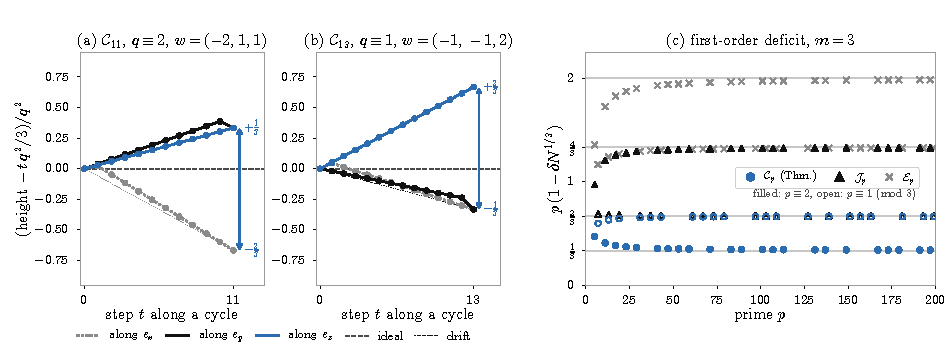
\includegraphics[width=\linewidth,height=0.5\textheight,keepaspectratio]{figs/col_drift.pdf}}{\fbox{\parbox{0.9\textwidth}{\centering figure \texttt{col\_drift} pending}}}
\caption{\colDriftCaption\interactive{anatomy.html}}
\label{fig:drift}
\end{figure}

\subsection{The holonomy, and the optimum among column nets}
No column point set beats the cubic value $\delta N^{1/3}=1$, and among those that are $(0,3,3)$-nets the column nets of Definition~\ref{def:col} are optimal.

\begin{corollary}[Column ceiling]\label{cor:colceil}
Every column point set in base $q\ge2$ has $g\le\frac13q^2$ in Theorem~\ref{thm:colmin}, i.e. toroidal minimum distance at most $q^2$ at integer scale $q^3$: $\delta N^{1/3}\le1$.
\end{corollary}

\begin{proof}
If $g>\frac13q^2$, every step value $\Delta_i([n])$ has distance more than $\frac13q^2$ from $\frac23q^2+q^2\Z$, so its residue modulo $q^2$ lies in the open interval $(0,\frac13q^2)$. The three steps $[n]\to[n+\e_x]\to[n+\e_x+\e_y]\to[n+\mathbf 1]=[n]$ have step values that sum to $0$, so their residues sum to a multiple of $q^2$; but that sum lies in $(0,q^2)$.
\end{proof}

So a net at $m=3$ with $\delta N^{1/3}>1$ cannot be a column point set. Proposition~\ref{prop:twocoset} shares the geometric digit between two coordinates only, and Proposition~\ref{prop:wnet} uses a layer of rank one, not of the column form $\mathbf 1a^{\!\top}$, under which all three coordinates still wrap together (Section~\ref{sec:wnet}).

\begin{theorem}[Column optimum]\label{thm:O}
Let $q\ge2$.
\begin{enumerate}
\item A column point set, with the set of columns $\mathbb T$ and the heights $\varphi$ of Section~\ref{sec:m3}, is a $(0,3,3)$-net in base $q$ if and only if $\varphi$ is a bijection from $\mathbb T$ onto $\{0,\dots,q^2-1\}$ and $\lfloor\varphi/q\rfloor$ is injective on every line of $\mathbb T$ in the directions $[\e_x],[\e_y],[\e_z]$.
\item If $q$ is even, no column point set is a $(0,3,3)$-net in base $q$.
\item If $q\ge5$ is odd and $3\nmid q$, every column point set that is a $(0,3,3)$-net in base $q$ has toroidal minimum distance $d$ with $d^2\le d^2(\mathcal C_q)$, the value of Theorem~\ref{thm:col}(2); equivalently $\eta\ge\frac13q+1$ for $q\equiv2$ and $\eta\ge\frac23q$ for $q\equiv1\pmod3$, where $\eta=\frac13q^2-g$.
\end{enumerate}
\end{theorem}

\begin{proof}
(1) The point of cell $n$ has the digits $n_c$, $\lfloor\varphi/q\rfloor$, $\varphi\bmod q$ in every coordinate. The box of shape $(1,1,1)$ holds one point per cell. A box with depth $3$ on $c$ prescribes $n_c$ and $\varphi$; the $q^2$ cells with a given $n_c$ meet every column exactly once ($n+t\mathbf 1$ for the one $t$ with $n_c+t$ given), so these boxes hold one point each if and only if $\varphi$ is a bijection. A box with depth $2$ on $c$, $1$ on $c'$ and $0$ on $c''$ prescribes $n_c$, $n_{c'}$ and $\lfloor\varphi/q\rfloor$; the $q$ cells with given $n_c,n_{c'}$ form a line in the direction $\e_{c''}$, whose columns form a line of $\mathbb T$ in the direction $[\e_{c''}]$, and every such line of $\mathbb T$ arises. These are all box shapes.

(2) Identify $\mathbb T$ with $(\Z/q\Z)^2$ by $[n]\mapsto(n_x-n_z,n_y-n_z)$; the lines in the directions $[\e_x]$, $[\e_y]$, $[\e_z]$ become the horizontal lines, the vertical lines and the lines of slope $1$ of $(\Z/q\Z)^2$. A level set $\{\lfloor\varphi/q\rfloor=v\}$ has $q$ elements and meets each of these lines once, by (1). So it is the graph of a permutation $\pi$ of $\Z/q\Z$ (once on every horizontal and every vertical line) such that $y\mapsto\pi(y)-y$ is a permutation too (once on every line of slope $1$). Then $\sum_y(\pi(y)-y)\equiv0$, while the sum over all residues is $\frac q2\not\equiv0\pmod q$ for even $q$. In other words, $y\mapsto\pi(y)-y$ is a complete mapping of $\Z/q\Z$, and this is the classical argument that a cyclic group of even order has none \cite[Thm.~1 and its corollary]{Pai51}; more generally, no finite group with a nontrivial cyclic Sylow $2$-subgroup has one \cite[Thm.~5]{HP55}. In the language of Latin squares, (1) says that each level set is a transversal of the cyclic Latin square $(a,b)\mapsto b-a$, and that the array $\lfloor\varphi/q\rfloor$ on $(\Z/q\Z)^2$ is a Latin square orthogonal to it.

(3) Put $\eta=\frac13q^2-g$. By Corollary~\ref{cor:colceil}, $0\le\eta\le\frac13q^2$, and by Theorem~\ref{thm:colmin} $d^2=q^4-2q^2\eta+3\eta^2$, which decreases in $\eta$ on this interval and equals $d^2(\mathcal C_q)$ at $\eta_0=\frac13q+1$ ($q\equiv2$) resp.\ $\eta_0=\frac23q$ ($q\equiv1$). So it suffices to show $\eta\ge\eta_0$. Suppose $\eta<\eta_0$.

\emph{Then $\eta<\frac1{12}q^2$.} For $q\ge8$ this holds because $\eta_0\le\frac1{12}q^2$. For $q=5$ and $7$: $3g=|3U+q^2|$ for an integer $U$, which is not divisible by $3$ since $q^2\equiv1\pmod3$, so $3\eta=q^2-3g\equiv0$ or $2\pmod3$; hence $\eta<\frac83$ gives $\eta\le2<\frac{25}{12}$ at $q=5$, and $\eta<\frac{14}3$ gives $\eta\le4<\frac{49}{12}$ at $q=7$.

\emph{Windows and triangles.} Every step value has distance at least $\frac13q^2-\eta$ from $\frac23q^2+q^2\Z$, so it has a unique representative $u$ in the window $[-\eta,\frac13q^2+\eta]$ modulo $q^2$ (narrower than the window of Section~\ref{sec:excess}). As $[\e_x]+[\e_y]+[\e_z]=0$ in $\mathbb T$, for every column and every order of the three directions the three steps around the triangle $[n]\to[n+\e_i]\to[n+\e_i+\e_{i'}]\to[n]$ have values summing to $0$, so their representatives sum to a multiple of $q^2$ in $[-3\eta,q^2+3\eta]$, i.e. to $0$ or $q^2$. In a triangle with sum $0$ every $u$ lies in $[-\eta,2\eta]$, and in one with sum $q^2$ every $u$ lies in $[\frac13q^2-2\eta,\frac13q^2+\eta]$; as $\eta<\frac1{12}q^2$ these ranges are disjoint, so two triangles that share a step have the same sum. The step $([n],i)$ shares a triangle with $([n+\e_i],i')$ for both $i'\ne i$, and two such moves give $([n+\e_i+\e_{i'}],i)=([n-\e_{i''}],i)$; and the classes $[\e_{i''}]$, $i''\ne i$, generate $\mathbb T$; so all steps are connected through shared triangles, and all triangles have the same sum. Sum $q^2$ means that every step is close to $\frac13q^2$, the configuration of the reflected cube $H\Z^3$; sum $0$ means that every step is close to $0$, the configuration of $\Z^3$.

\emph{Sum $q^2$ (the reflected cube).} Put $\xi=u-\frac13q^2\in[-2\eta,\eta]$, the excess; then $\operatorname{dist}(u,\frac23q^2+q^2\Z)=\frac13q^2-\xi$, so $\eta$ is the largest excess, and every triangle has excess sum $0$. The class $[\e_i]$ has order $q$ in $\mathbb T$, so the steps in the direction $\e_i$ form $q$ cycles $\gamma$ of length $q$. Along a cycle the step values telescope to $0$, so $\sum_{\gamma}u\in q^2\Z$, and the \emph{cycle excess} $\Xi_\gamma=\sum_\gamma\xi\in q^2\Z-\frac13q^3$. Summing the excess over the triangles $[n]\to[n+\e_x]\to[n+\e_x+\e_y]\to[n]$ for all $[n]\in \mathbb T$ counts every step once, so the $3q$ cycle excesses sum to $0$. Also $-2q\eta\le\Xi_\gamma\le q\eta$.
If $q\equiv1\pmod3$, then $\Xi_\gamma=q^2z_\gamma-\frac13q^2$ with integers $z_\gamma$ (as $\frac13q^3\equiv\frac13q^2$), and the cycle excesses sum to $0$ only if $\sum_\gamma z_\gamma=q$. So some $z_\gamma\ge1$, $\Xi_\gamma\ge\frac23q^2$, and $q\eta\ge\frac23q^2$: $\eta\ge\frac23q$, a contradiction.
If $q\equiv2\pmod3$, then $\Xi_\gamma=q^2z_\gamma-\frac23q^2$ and $\sum_\gamma z_\gamma=2q$. Every excess lies in $\Z+\frac23$ (as $u\in\Z$ and $\frac13q^2\in\Z+\frac13$), and so does $\frac13q$; hence $\eta<\frac13q+1$ gives $\eta\le\frac13q$, and then every $\Xi_\gamma\in[-\frac23q^2,\frac13q^2]$, i.e. $\Xi_\gamma\in\{-\frac23q^2,\frac13q^2\}$. A cycle excess $\frac13q^2\le q\eta$ forces $\xi=\eta=\frac13q$ on each step of its cycle, and a cycle excess $-\frac23q^2\ge-2q\eta$ forces $\xi=-2\eta=-\frac23q$ on each step. So every step has $u=\frac13q(q+1)$ or $\frac13q(q-2)$, a multiple of $q$, and $\varphi$ is constant modulo $q$ on $\mathbb T$. This contradicts (1): $\varphi$ takes every value in $\{0,\dots,q^2-1\}$.

\emph{Sum $0$ (the cube).} Now $u\in[-\eta,2\eta]$ and $\operatorname{dist}(u,\frac23q^2+q^2\Z)=u+\frac13q^2$, so $\min u=-\eta$. The cycle sums $\sum_\gamma u$ lie in $q^2\Z$ and add up to $0$. If one of them is nonzero, one is at most $-q^2$; it is at least $-q\eta$, so $\eta\ge q$. Otherwise every cycle closes: the partial sums $S_t$ of $u$ along a cycle are integers with $S_t\equiv\varphi(c_t)-\varphi(c_0)\pmod{q^2}$, where $c_t$ are its columns. By (1) the $q$ values $\varphi(c_t)$ lie in $q$ different blocks $[kq,kq+q)$, so the $q$ values $\varphi(c_0)+S_t$ meet all $q$ blocks modulo $q^2$; an interval of integers of length $\mathrm{rg}$ meets at most $\mathrm{rg}/q+2$ of them, so the range of the walk is $\mathrm{rg}\ge q(q-2)$. Here $\eta>0$, since $\eta=0$ would make every step value $0$ and $\mathrm{rg}=0<q(q-2)$. A closed walk whose up-steps are at most $2\eta$ and whose down-steps are at least $-\eta$ needs at least $\mathrm{rg}/(2\eta)+\mathrm{rg}/\eta$ steps, so $q\ge3\,\mathrm{rg}/(2\eta)$ and $\eta\ge\frac32(q-2)$. Both $q$ and $\frac32(q-2)$ are at least $\frac23q\ge\eta_0$ for $q\ge4$, a contradiction.

Equality holds for $\mathcal C_q$ by Theorem~\ref{thm:col}(2).
\end{proof}

So among column nets the first-order deficits $\frac13$ ($q\equiv2$) and $\frac23$ ($q\equiv1\pmod3$) are optimal, and $\mathcal C_q$ attains the optimum exactly, second order included. Within the class this answers why the deficits are what they are. Whether some digital $(0,3,3)$-net that is not a column point set has a deficit below $\frac13$ (resp.\ $\frac23$) is open (Remark~\ref{rem:open}(5)).

\emph{The holonomy.} The ideal step $\frac13q^2$ of the reflected cube cannot close up: $q$ steps around a cycle of $\mathbb T$ give $\frac13q^3$, but the heights live modulo $q^2$, and $\frac13q^3\notin q^2\Z$ when $3\nmid q$. So every cycle carries a forced total excess, its \emph{holonomy}, and some step must carry at least its share. Formally, in the case of sum $q^2$ the excess is a closed $1$-form on the triangulated torus $\mathbb T$ (its sum around every triangle vanishes), and its sums around the cycles of $\mathbb T$ are prescribed modulo $q^2$. For $q\equiv2\pmod3$ every cycle total is $\frac13q^2$ modulo $q^2$ (the smallest choices are $\frac13q^2$ and $-\frac23q^2$), and as the totals add up to zero, some cycle has at least $\frac13q^2$; for $q\equiv1$ every cycle total is $-\frac13q^2$ modulo $q^2$, and the totals add up to zero only if some cycle has at least $\frac23q^2$ (the balance $\sum_\gamma z_\gamma=q$ of the proof). Spread over the $q$ steps of that cycle, this is at least $\frac13q$ resp.\ $\frac23q$ per step: the deficits $\frac13$ and $\frac23$ are these per-step shares of a forced holonomy. (The $+1$ in $\eta\ge\frac13q+1$ is not holonomy but the net property.) For the digital nets of Lemma~\ref{lem:drift} with $|w_c|\le2$ (Lemma~\ref{lem:drift}(2)) the total excess of a cycle in the direction $\e_i$ is $\frac13q^2w_i$, so the drift $\frac13qw_i$ is exactly the per-step share of the holonomy, and the jitter decides how evenly the cycle spreads it. As a rule for constructions: spread the forced excess evenly over the directions that attain the minimum distance, and give the largest third-digit steps to the directions with the smallest drift. Theorem~\ref{thm:O} proves this rule optimal for column nets; beyond them it is a heuristic. Two comparisons show what each term does (Figure~\ref{fig:drift}(c)). Fixing the drift at $w=-\gamma\mathbf 1$, $\gamma\in\{1,2\}$, by the shared second digit $\lfloor q/3\rfloor\Sigma n$ (its row $\lfloor q/3\rfloor\mathbf 1$ sums to $3\lfloor q/3\rfloor\not\equiv0\pmod q$, so the shared digit is not constant on a column, and the points do not lie on columns) and choosing only the jitter residues, at every prime $q=p$, $5\le p\le199$, the third digit $\frac12(-n_c-n_{c+1}+n_{c+2})$ gives $p(1-\delta N^{1/3})$ close to $\frac23$ ($p\equiv1$) and $\frac43$ ($p\equiv2$), and the third digit $n_{c+1}$ close to $\frac43$ and $2$ (computed exactly at every such prime; within $0.06$ of these values for every prime $53\le p\le199$); the column nets reach $\frac23$ ($p\equiv1$) and $\frac13$ ($p\equiv2$).

\emph{Dimension five.} The same bookkeeping applies to half-integer layers (Section~\ref{sec:halfms}). There the holonomy is a parity: $p$ steps of $\frac p2$ do not close up modulo the odd $p$. The net property excludes the cheapest sign patterns, a skew-symmetric layer balances the steps with all coordinates moving, and a second offset row with few harmful entries keeps the jitter off the steps that attain the minimum. Theorem~\ref{thm:D} shows that the drift $\mathrm{dr}$ of such a layer is at least $\frac{17}2$, where $\mathrm{dr}$ is measured in units of $1/p$ of a cell on the squared length, $(\delta N^{1/5})^2\approx\frac54-\mathrm{dr}/p$; a layer attains it, and with a suitable second row it gives $(0,5,5)$-nets with $\delta N^{1/5}>1$ for every prime $p\ge37$ (Proposition~\ref{prop:half5}).

\section{One point per cube: cube tilings and the value 1}\label{sec:whylat}
The lattice picture uses only that the geometric digit is linear in the cell digits. This section makes precise what that linearity forces: offsets that are affine in the cell between wraps, so locally a lattice, but broken at the slip planes where a geometric digit wraps, so globally not a lattice. It also shows what the cube cells of the resolutions $m=sk$ cost. Call the position of a point inside its cell its \emph{phase}; for a digital net it is, to first order, $r/q$ with $r$ the geometric digits. By the cube-tiling theorems of Haj\'os and Keller, configurations with one point per unit cube whose phases vary independently are no better than $\Z^s$ (Proposition~\ref{prop:cube}). In Lemma~\ref{lem:hom} and Corollary~\ref{cor:linoff} only, the digits of an integer $0\le P<q^j$ are counted from the least significant one: $P=\sum_{i<j}d_i(P)\,q^i$.

\begin{lemma}[Additive digit functionals]\label{lem:hom}
Let $q\ge2$, $j\ge1$, $\beta_0,\dots,\beta_{j-1}\in\Z/q\Z$, and $\phi(P)=\sum_{i<j}\beta_i\,d_i(P)$ for $P\in\Z/q^j\Z$ (digits of the representative in $[0,q^j)$). Then $\phi$ is a homomorphism $\Z/q^j\Z\to\Z/q\Z$ if and only if $\beta_i=0$ for every $i\ge1$.
\end{lemma}

\begin{proof}
If $\beta_i=0$ for $i\ge1$, then $\phi(P)=\beta_0\,(P\bmod q)$, a homomorphism. Conversely, a homomorphism on the cyclic group $\Z/q^j\Z$ satisfies $\phi(P)=P\,\phi(1)=\beta_0P=\beta_0\,d_0(P)$ in $\Z/q\Z$; at $P=q^i$, $i\ge1$, this gives $\beta_i=\phi(q^i)=\beta_0\,d_0(q^i)=0$.
\end{proof}

So a linear function of the digits is additive in the integer only through the lowest digit; at every higher digit, carries break additivity. The geometric digit is a linear function of the last cell digits, one level above it: it is additive, hence affine and lattice-like, between carries and wraps, and it breaks where they occur.

\begin{corollary}[Linear offsets]\label{cor:linoff}
Let $q\ge2$.
\begin{enumerate}
\item[(a)] \emph{One level.} Let a set of integer vectors $Y\in\Z^s$ consist of all $Y$ whose lowest base-$q$ digits $(Y_c\bmod q)_c$ satisfy a system of linear equations over $\Z/q\Z$, with solution set $y_0+C$ for a linear code $C\subset(\Z/q\Z)^s$, all higher digits being free. Then the set is the coset $y_0+C+q\Z^s$ of the Construction~A lattice $C+q\Z^s$.
\item[(b)] \emph{Two levels.} For an $s\times s$ matrix $B$ over $\Z/q\Z$ let $\mathcal D_B=\{q\ell+(B\ell\bmod q):\ell\in\{0,\dots,q-1\}^s\}\subset(\Z/q^2\Z)^s$ (the \emph{two-digit set} of $B$; $\ell$ plays the part of the last cell digits), with $B\ell\bmod q$ taken in $[0,q)^s$. Then $\mathcal D_B$ is a subgroup if and only if $Bc\equiv0\pmod q$ for every carry vector $c=(\lfloor(v_i+v'_i)/q\rfloor)_i$ of two vectors $v,v'\in\{B\ell\bmod q\}$. If $B$ is invertible, $\mathcal D_B$ is not a subgroup.
\item[(c)] \emph{Locally a lattice.} Let a digital net over $\Z/q\Z$ be in graph form with depths $(k,\dots,k)$ and geometric layer $\tilde M$, and let the cells $n$, $n'$ differ only in their last level, by $n'-n=E\in\Z^s$ (no carry). If the geometric digits $r$ of $n$ satisfy $r+\tilde ME\in[0,q)^s$, then in cell units the points of $n'$ and $n$ differ by $(I+\tilde M/q)E+(f'-f)/q$, with $f,f'\in[0,1)^s$ the contributions of the deeper digits.
\end{enumerate}
\end{corollary}

\begin{proof}
(a) The set of $Y\in\Z^s$ with $Y\bmod q\in y_0+C$ is $y_0+C+q\Z^s$. (b) Let $Y=q\ell+v$ and $Y'=q\ell'+v'$ be in $\mathcal D_B$, and let $c$ be the carry vector of $v,v'$. Then $Y+Y'=q(\ell+\ell'+c)+(v+v'-qc)$ with $v+v'-qc\in[0,q)^s$, and $v+v'\equiv B(\ell+\ell')$; so $Y+Y'\in\mathcal D_B$ if and only if $Bc\equiv0$. A nonempty finite subset of a group that is closed under addition is a subgroup. If $B$ is invertible, its image contains $v=v'=\lceil q/2\rceil\e_i$, whose carry vector is $\e_i$; then $B\e_i\equiv0$ would be needed, which is false. (c) Only the last digits of the cells change, so $r$ changes by $\tilde ME$ modulo $q$, and $r'=r+\tilde ME$ exactly since both sides lie in $[0,q)^s$; the cell digits change by $E$.
\end{proof}

At $m=s$, $\mathcal D_B$ is the set of the first two digits of all points of the graph form with geometric layer $B$, so (b) says that the configuration of an invertible layer is never a lattice: it is a lattice coset cut at slip planes (Figure~\ref{fig:arcwhylat}). What digitality forces is therefore \emph{linear offsets}: by (c), away from the wraps the offset of a point is an affine function of its cell, so locally the points form a coset of the lattice $(I+\tilde M/q)\Z^s$ up to the jitter. Finite unions of lattice cosets are not excluded, and they occur: $D_s^+$ for odd $s$ and the configuration of Proposition~\ref{prop:twocoset}.

At $m=s$ (one cell digit per coordinate) write $B$ for the geometric layer modulo $p$. The phase of the cell $n$ is then given by its geometric digits $r(n)=Bn\bmod p$, and the phase decides which coordinates wrap on a step (Lemma~\ref{lem:phase}(i)). An invertible layer realizes every wrap pattern, and every square minor of the layer of a $(0,sk,s)$-net with disjoint row and column sets is a unit (Lemma~\ref{lem:phase}(ii)).

\begin{lemma}[Wrap patterns; rank of the layer]\label{lem:phase}
\begin{enumerate}
\item[(i)] Let $p$ be a prime and consider a graph form over $\F_p$ with depths $(1,\dots,1)$: coordinate $c$ of the point with index $n\in\F_p^s$ has the digits $n_c$, $r_c(n)=(Bn)_c$ and deeper digits, with $B\in\F_p^{s\times s}$. For $E\in\Z^s$ let $\beta=BE\bmod p\in\{0,\dots,p-1\}^s$ and $n'\equiv n+E$. Then $r(n')=r(n)+\beta-p\omega$ with $\omega_c=[r_c(n)+\beta_c\ge p]$, and $\omega_c=0$ whenever $\beta_c=0$. If $B$ is invertible, then every $\omega\in\{0,1\}^s$ with $\omega_c=0$ whenever $\beta_c=0$ is the wrap vector of some cell $n$.
\item[(ii)] Let a digital $(0,sk,s)$-net over $\Z/q\Z$, $k\ge1$, be in graph form with depths $(k,\dots,k)$ and geometric layer $\tilde M$. For disjoint $T,Z\subset\{1,\dots,s\}$ with $|T|=|Z|$, $\det\tilde M_{T,Z}$ is a unit of $\Z/q\Z$. In particular $\tilde M$ has rank at least $\lfloor s/2\rfloor$ modulo every prime factor of $q$.
\end{enumerate}
\end{lemma}

\begin{proof}
(i) $r(n')\equiv B(n+E)\equiv r(n)+\beta$, and $r(n')\in[0,p)^s$, which gives $\omega$; if $\beta_c=0$, then $r_c(n)+\beta_c<p$. If $B$ is invertible, take $n=B^{-1}y$ with $y_c=p-1$ if $\omega_c=1$ (then $\beta_c\ge1$ and $y_c+\beta_c\ge p$) and $y_c=0$ if $\omega_c=0$. (ii) The box with depths $k+1$ on $T$, $k-1$ on $Z$ and $k$ elsewhere has total depth $sk$; by Lemma~\ref{lem:box} its minor is, up to sign, the determinant of the first offset rows of $T$ on the last level of $Z$, which is $\det\tilde M_{T,Z}$ modulo $q$, and by Lemma~\ref{lem:nie} it is a unit. Disjoint $T$, $Z$ of size $\lfloor s/2\rfloor$ exist.
\end{proof}

So in (i), at the representative with cell difference $E$, the points of $n$ and $n'$ differ in cell units by $E+b-\omega$, $b=\beta/p$, plus less than $1/p$ per coordinate of jitter. We call $b\in[0,1)^s$ the \emph{glue} of the step $E$: to first order, the change of the phase on the step, in cell units and modulo $1$. Call the wraps of a layer \emph{free} if every wrap vector allowed by (i) occurs, as for every invertible layer. Then, up to the jitter, the minimum distance is the least \emph{fully folded length} over the steps $E\ne0$: the length $|E+b-\omega|$ minimized over the allowed wrap vectors $\omega$, whose coordinate $c$ is $\min(|E_c+b_c|,|E_c+b_c-1|)$ if $\beta_c\ne0$ and $|E_c|$ if $\beta_c=0$. Part (ii) contains the $2\times2$ minors used for Theorem~\ref{thm:L}.

\begin{remark}[Glue under free wraps]\label{rem:glue}
A coordinate with $E_c=0$ and $\beta_c\ne0$ contributes $\min(b_c,1-b_c)\le\frac12$ to the fully folded length, with equality only for $b_c=\frac12$: a step keeps its full length under free wraps only if its glue in each coordinate that does not move is $\frac12$, the only value that is its own negative modulo $1$. So half-integer layers do not need the wraps of different coordinates to be correlated: for odd $s$ the differences between the two cosets of $D_s^+$ fill $(\Z+\frac12)^s$, a set that free wraps (integer changes of single coordinates) map to itself, so these steps keep a length of at least $\sqrt s/2$, and the relaxation of Proposition~\ref{prop:Hk} at $k=1$, which allows every wrap, tends to $\min(\sqrt s/2,\sqrt2)$ for dominant layers. The glue $\frac13\mathbf 1$ of the reflected cube does not survive: with free wraps the step $E=\e_1$ of the layer $\frac p3\mathbf 1\mathbf 1^{\!\top}$ would have fully folded length $1/\sqrt3=.5773\ldots$, and bounded perturbations of the equal rows $\mathbf 1a^{\!\top}$ of the column nets make the wraps independent (computed instance: Figure~\ref{fig:arcwhylat}(b)). Wraps that are correlated across coordinates because the layer is singular (\emph{locked} wraps, Section~\ref{sec:wnet}) are needed otherwise: the column nets (Theorem~\ref{thm:col}) share one geometric digit among all three coordinates, Proposition~\ref{prop:twocoset} between two, and in Proposition~\ref{prop:wnet} a layer of rank one locks all three, one coordinate reading half of the digit of the others; literally equal rows exist only at $(s,m)=(3,3)$ (Lemma~\ref{lem:shared}). Locked wraps are what produces the coherent phases defined before Proposition~\ref{prop:cube}. The half-integer rule concerns coordinates whose wraps are free: a coordinate whose wraps are locked to those of the others can carry other glue and a step longer than one cell along its own axis (in the net $\mathcal W_p$ of Section~\ref{sec:wnet}, the glue $\frac12+3\varepsilon$ and the step $1+2\varepsilon$ along $\e_z$, with $\varepsilon=\rho/(2p)$). The rule concerns the length of a single step under free wraps; it is a heuristic for the choice of glue, not an optimality statement for the minimum, even for free coordinates (the remark on $\sqrt{233}/15$ in Section~\ref{sec:wnet}).
\end{remark}

\begin{figure}[tbp]
\centering
\arcfig{arc_whylat}
\caption{\arcWhyLatCaption}
\label{fig:arcwhylat}
\end{figure}

At the resolutions $m=sk$ the cells are cubes. Call $S\subset\R^s$ a \emph{one-per-cube set} if every unit cube $n+[0,1)^s$, $n\in\Z^s$, contains exactly one point of $S$, and \emph{periodic} with period lattice $\Pi$ (of full rank) if $S+\Pi=S$; write $\mu(S)$ for its minimum distance. The \emph{phase group} of a lattice $L$ is $Y=(L+\Z^s)/\Z^s\subset(\R/\Z)^s$, the set of fractional offsets (the phases) of its points. Say that the phases of $L$ \emph{vary independently} if $Y$ is dense in $(\R/\Z)^s$ (equivalently, $\Z^s+L$ is dense), or finite and equal to $\pi_1(Y)\times\dots\times\pi_s(Y)$, the product of its projections to the coordinate circles; the lattices in $\mathbb Q^s$ are those with a finite phase group, and we do not treat lattices whose phase group is neither dense nor finite. A lattice whose phase group is finite and smaller than the product of its projections has \emph{coherent} phases. For every $(0,sk,s)$-net $P$ in base $q$, digital or not, $S=q^k(P+\Z^s)$ is a periodic one-per-cube set with $\Pi\supset q^k\Z^s$, and $\min(\delta N^{1/s},q^k)=\mu(S)$ for the toroidal $\delta$ of $P$.

\begin{proposition}[One point per cube]\label{prop:cube}
Let $S$ be a periodic one-per-cube set in $\R^s$ with period lattice $\Pi$.
\begin{enumerate}
\item[(i)] If $S=L$ is a lattice and $\Z^s+L$ is dense in $\R^s$, then $L$ contains a unit vector $\e_c$; so $\mu(L)\le1$.
\item[(ii)] If $S=L\subset\mathbb Q^s$ is a lattice whose phase group $Y$ equals $\pi_1(Y)\times\dots\times\pi_s(Y)$, the product of its projections to the coordinate circles, then $L$ contains a unit vector $\e_c$; so $\mu(L)\le1$.
\item[(iii)] If $s\le7$ and $\Z^s+\Pi$ is dense in $\R^s$, then two points of $S$ differ by a unit vector; so $\mu(S)\le1$.
\item[(iv)] If $S-x\subset\mathbb Q^s$ for some $x$, all squared distances in $S$ are rational. Hence $\mu(S)<(4/3)^{1/4}$ for $s=2$ and $\mu(S)<2^{1/6}$ for $s=3$, the optimal packing values at density $1$; and for $4\le s\le7$, $\mu(S)$ differs from the value of the densest known packing at density $1$ ($D_4$, $D_5$, $E_6$, $E_7$, with squared minima $\sqrt2$, $2^{3/5}$, $2\cdot3^{-1/6}$, $2^{6/7}$).
\end{enumerate}
\end{proposition}

\begin{proof}
Let $f(x)=\#\bigl(S\cap(x+[0,1)^s)\bigr)$. Then $f(x+\pi)=f(x)$ for $\pi\in\Pi$ and $f(n)=1$ for $n\in\Z^s$, so $f=1$ on $\Z^s+\Pi$. For every $x$ there is $\varepsilon>0$ such that $f$ is constant on $x-[0,\varepsilon)^s$: $S$ is locally finite, so we may choose $\varepsilon$ below every positive difference $x_c-\sigma_c$ and $x_c+1-\sigma_c$ for the finitely many $\sigma\in S$ near the cube, and then shifting the cube by $-t$, $t\in[0,\varepsilon)^s$, neither adds nor removes a point. If $f\equiv1$, the cubes $\sigma+(-1,0]^s$, $\sigma\in S$, tile $\R^s$, since $x\in\sigma+(-1,0]^s$ if and only if $\sigma\in x+[0,1)^s$.
(i) Density gives a point of $\Z^s+L$ in every $x-[0,\varepsilon)^s$, so $f\equiv1$, and the cubes form a lattice tiling. By Haj\'os's theorem (Minkowski's conjecture) \cite{Haj42} two of them share a facet, so $L$ contains some $\e_c$.
(ii) For each $c$, $\pi_c(L)+\Z$ is a finitely generated subgroup of $\mathbb Q$ containing $\Z$, hence equal to $\frac1{e_c}\Z$ for an integer $e_c\ge1$. For $x_c\in(\frac{j-1}{e_c},\frac j{e_c}]$ and $\sigma\in L$ the condition $x_c\le\sigma_c<x_c+1$ is equivalent to $\frac j{e_c}\le\sigma_c\le\frac{j-1}{e_c}+1$, which does not depend on $x_c$; so $f$ is constant on every box $\prod_c(\frac{j_c-1}{e_c},\frac{j_c}{e_c}]$, and its value there is that at the corner $(j_c/e_c)_c$. By hypothesis the corner lies in $\Z^s+L$, so $f\equiv1$, and Haj\'os's theorem applies as in (i).
(iii) As in (i), $f\equiv1$ and the cubes $\sigma+(-1,0]^s$ tile $\R^s$. Keller's conjecture holds for $s\le7$ (Perron \cite{Per40} for $s\le6$, Brakensiek, Heule, Mackey and Narv\'aez \cite{BHMN20} for $s=7$): two cubes of the tiling share a complete facet, so their corners differ by some $\e_c$.
(iv) The differences are rational vectors. As $S$ is a finite union of $\Pi$-cosets, $\mu(S)$ is a minimum over the finitely many $\Pi$-orbits of pairs, so it is attained and $\mu(S)^2$ is rational. A periodic set of density $1$ with minimum $\mu$ is a packing of balls of radius $\mu/2$ with density $\mathrm{vol}(B_{\mu/2})$, so $\mu^2$ is at most $4\vartheta_s^{2/s}$ with $\vartheta_s$ the optimal centre density; this is $2/\sqrt3$ for $s=2$ \cite[Ch.~1]{CS99} and $2^{1/3}$ for $s=3$ \cite{Hal05}, both irrational. The four squared minima for $4\le s\le7$ are $4\vartheta_s^{2/s}$ with the centre densities $\frac18$, $\frac1{8\sqrt2}$, $\frac1{8\sqrt3}$, $\frac1{16}$ \cite{CS99}, and they are irrational.
\end{proof}

Parts (i)--(iii) say that a one-per-cube lattice whose phases vary independently, and for $s\le7$ any periodic one-per-cube set with dense phases, is no better than $\Z^s$. So a rational one-per-cube lattice with minimum above $1$ has coherent phases. $H\Z^3$ and $D_s^+$ for even $s$ have coherent phases, and $D_s^+$ beats the cubic value for even $s\ge6$. The configuration $\Gamma$ of Section~\ref{sec:twocoset} and $D_s^+$ for odd $s\ge5$, both unions of two lattice cosets, beat it too, and so do, in the limit, the rank-one nets of Proposition~\ref{prop:wnet}, whose phases lie on one line.

These statements concern idealized configurations. For a net $P$ in a fixed base, $S=q^k(P+\Z^s)\subset q^{k-m}\Z^s$ is rational, so $\Z^s+\Pi$ is discrete, and (i) and (iii) never apply to the net itself; they apply to idealized models of its local configuration, the sets $\{n+\{An+y\}:n\in\Z^s\}$ obtained in the limit $q\to\infty$ with $\tilde M/q\to A$, when their phases are irrational. Part (ii) applies to rational lattices, among them the limits as $q\to\infty$ of the local configurations ($\Z^s$ in regime I of Section~\ref{sec:prelim}, $H\Z^3$, and $D_s^+$ for even $s$), and to a net itself only when $S$ is a lattice; at $m=s$ the first two digits of an invertible layer never form a group (Corollary~\ref{cor:linoff}(b)). Part (iv) applies to every net. For $s\ge8$ part (iii) says nothing (Keller's conjecture fails \cite{LS92,Mac02}), and at $s=8$ the squared minimum $2$ of $E_8$ is rational; Theorem~\ref{thm:HL} reaches it in the limit. Part (iv) needs $S\subset x+\mathbb Q^s$: for a periodic set whose period lattice is merely rational, cross-coset distances can be irrational.

\begin{remark}[What the cube costs; computed]\label{rem:cubecost}
The largest minimum of a periodic one-per-cube set is not known. In dimension three an exhaustive enumeration of the lattices of covolume $1$ in $\frac1e\Z^3$, $e\le11$, finds one-per-cube lattices with minimum up to $\sqrt{29/25}=1.0770\ldots$ (computed), for instance the lattice with basis $\tfrac1{5}(3,-4,-2)$, $\tfrac1{10}(6,2,-9)$, $\tfrac1{2}(1,0,2)$. It has covolume $1$; its Gram matrix $100^{-1}\left(\begin{smallmatrix}116&56&-10\\56&121&-60\\-10&-60&125\end{smallmatrix}\right)$ is Minkowski-reduced, so its minimum is $\sqrt{116/100}$; and a finite check over one period shows that every unit cube holds exactly one of its points. So the largest minimum lies between $1.0770$ and $2^{1/6}=1.1224\ldots$ \cite{Hal05}. The maximizers found have offsets that are not affine modulo $1$ in the cell, so no digital net realizes them through its geometric digit (Corollary~\ref{cor:linoff}(c)); the best digital value at $m=3$ in this paper is $\sqrt{281}/16=1.0476\ldots$ (Proposition~\ref{prop:wnet}). For $s\le9$, restricting to lattices is not known to lose anything: lattices hold the packing records there and are optimal for $s=3$, $8$ \cite{CS99,Hal05,Via17}. The constraints visible here are the \emph{cube constraint} (one point in every cube of side $q^{-k}$, at $m\equiv0\pmod s$), the linearity of the offsets and, in the frame orbit, Lemma~\ref{lem:CH}. The skeleton regime ($m\not\equiv0\pmod s$), whose cells are not cubes, is not bound by the cube constraint (Table~\ref{tab:S1E}).
\end{remark}

\emph{Scope.} What uses the linearity of the geometric digit: Lemma~\ref{lem:hom}, Corollary~\ref{cor:linoff} and Lemma~\ref{lem:phase}; Corollaries~\ref{cor:ceil3} and~\ref{cor:ceils} and Proposition~\ref{prop:P2}, whose proofs use that a carry-free step changes every offset digit by a constant; Theorem~\ref{thm:L} (box minors of the layer, and carry-free steps); and, inside the frame orbit, where the layer is a Cauchy matrix (Proposition~\ref{prop:Ns}), Lemma~\ref{lem:CH} and its consequences (Remark~\ref{rem:pm1}, Theorem~\ref{thm:O5}, Corollary~\ref{cor:frameid}, Proposition~\ref{prop:P}).

What holds for every net, digital or not: Proposition~\ref{prop:cube}, which applies to the periodic set $S$ of every $(0,sk,s)$-net within the limits stated after it, and the box count of Lemma~\ref{lem:shared}: if, for every point of a $(0,m,s)$-net in base $q$, the digits with index $k$ (counted from the most significant, as everywhere outside Lemma~\ref{lem:hom} and Corollary~\ref{cor:linoff}) of two coordinates agree, or one is a fixed function of the other, then $2(k+1)>m$. For nets that are not digital only these constraints and the other box conditions remain (Remark~\ref{rem:open}(11)).

\section{Beyond the cubic value: Euclidean skeletons and half-integer layers}\label{sec:large}
By Proposition~\ref{prop:cube}, a set with one point per unit cube can have minimum distance above the cubic value $1$ only if the phases of its points are correlated (coherent, in the idealized setting of that proposition). For an invertible layer every pattern of wraps occurs (Lemma~\ref{lem:phase}(i)), so a step to a neighbouring cell keeps its full length only if its glue is $\frac12$ in every coordinate that does not move (Remark~\ref{rem:glue}). Three ways above $1$ occur in this paper.
\begin{enumerate}
\item[(i)] \emph{Euclidean skeletons} (Section~\ref{sec:S1E}). At $m\not\equiv0\pmod s$ the cells are boxes, longer in the skeleton coordinates, not cubes, so the cube constraint does not apply (Section~\ref{sec:skel}). In the Euclidean norm the certified constants exceed $1$ at $m\equiv-1\pmod s$ at the large primes of Table~\ref{tab:S1E}; whether this persists for all large $p$ is open (Remark~\ref{rem:S1Elim}).
\item[(ii)] \emph{Locked wraps at $m=3$} (Sections~\ref{sec:twocoset} and~\ref{sec:wnet}). A singular layer can force coordinates to wrap together. In $\mathcal T_p$ two coordinates share one geometric digit, and the points lie on a union of two lattice cosets; in $\mathcal W_p$ the layer has rank one, and all three coordinates wrap together.
\item[(iii)] \emph{Half-integer layers} (Sections~\ref{sec:Pnohalf}--\ref{sec:halfms}). Layers whose entries are half-integers, read modulo $q$ via $\frac12\equiv(q+1)/2$, so that each centred entry is about $\pm q/2$ plus a bounded amount (regime III, Figure~\ref{fig:arclarge}), put the points locally on the packing $D_s^+$. For $k\ge2$ the frame orbit cannot provide them (Proposition~\ref{prop:P}: for rational designs, and over $\F_p$ for large $p$), but split frames give them at every resolution $m=sk$ (Theorem~\ref{thm:HL}); at $k=1$ no frame is needed (Section~\ref{sec:halfms}).
\end{enumerate}

\subsection{Euclidean skeletons}\label{sec:S1E}
\emph{Euclidean form.} The bound of Theorem~\ref{thm:S1}(1) measures the centred difference $a$ of the fine-cell positions of two points (Lemma~\ref{lem:skelred}) in the maximum norm. Every skeleton digit $S_z=\sum_d\kappa_dx_{d,k}$ with all $\kappa_d\ne0$ can be realized (Proposition~\ref{prop:skelcomp}(ii)), and in the Euclidean norm the best choice is not $\kappa_d=\rho^d$ (Remark~\ref{rem:codes}(c)).

\begin{proposition}[Euclidean form of Theorem~\ref{thm:S1}(1)]\label{prop:S1E}
Let $s\ge3$, let $p\ge s-1$ be a prime, $k\ge0$, $m=sk+s-1$, and let $\kappa_1,\dots,\kappa_{s-1}$ be units of $\F_p$. The recipe of Proposition~\ref{prop:skelcomp}(ii) on the frame of Definition~\ref{def:S1} gives a digital $(0,m,s)$-net over $\F_p$ with the skeleton digit $S_z=\sum_d\kappa_dx_{d,k}$, and every graph form with the depths $(k+1,\dots,k+1,k)$ and this skeleton digit satisfies, for the toroidal distance,
\[
\delta N^{1/s}\ \ge\ p^{-1/s}\lambda_{\mathrm{jit}}(\kappa)\ \ge\ p^{-1/s}\bigl(\lambda_2(\Lambda_\kappa)-\sqrt s\bigr),\qquad \lambda_{\mathrm{jit}}(\kappa)=\min_{0\ne a\in\Lambda_\kappa}\bigl\|(|a|-\mathbf 1)_+\bigr\|_2,
\]
where $\Lambda_\kappa=\{a\in\Z^s:a_z\equiv\sum_d\kappa_da_{x_d}\pmod p\}$ and $(|a|-\mathbf 1)_+$ is taken coordinatewise. (So $\lambda_{\mathrm{jit}}$ is the length of the shortest nonzero lattice vector after one fine cell of jitter is subtracted from each coordinate.)
\end{proposition}

\begin{proof}
The net property is Proposition~\ref{prop:skelcomp}(ii); the $s$ places of Definition~\ref{def:S1} are distinct because $p\ge s-1$. As in the proof of Theorem~\ref{thm:S1}(1), $P_z\equiv\sum_d\kappa_dP_{x_d}\pmod p$ for every point, and the centred difference $a\ne0$ of the fine positions of two distinct points lies in $\Lambda_\kappa$. By Lemma~\ref{lem:skelred}(i) in each coordinate $c$, the two points are at toroidal distance at least $(|a_c|-1)_+\varpi$ in coordinate $c$, so their distance is at least $\varpi\|(|a|-\mathbf 1)_+\|_2\ge \varpi\lambda_{\mathrm{jit}}(\kappa)$, and $\varpi N^{1/s}/N=p^{-1/s}$. Finally $|a|\le(|a|-\mathbf 1)_++\mathbf 1$ coordinatewise gives $\|(|a|-\mathbf 1)_+\|_2\ge\|a\|_2-\sqrt s$.
\end{proof}

For $\kappa_d=\rho^d$ some $|a_c|$ is at least $\rho$, so $\lambda_{\mathrm{jit}}\ge\rho-1$ and the proposition contains Theorem~\ref{thm:S1}(1). Every index-$p$ sublattice of $\Z^s$ without unit vectors is a $\Lambda_\kappa$ after a permutation of the coordinates: it is the kernel of a functional $h$ modulo $p$, it contains no unit vector exactly when $h$ has full weight (all entries nonzero modulo $p$), and then $h$ can be scaled to $h_z=-1$. So the proposition can use the best of these lattices. Table~\ref{tab:S1E} lists certified values for searched $\kappa$; $\lambda_{\mathrm{jit}}^2$ is an integer, computed exactly by lattice reduction and complete enumeration and also checked in Lean (Appendix~\ref{app:formal}). At $p=1009$ they already beat Table~\ref{tab:skel} for $s=3,4,5$. The limit of the certified values as $p\to\infty$ is discussed in Remark~\ref{rem:S1Elim}.

\begin{table}[tbp]
\centering\small\setlength{\tabcolsep}{4pt}
\begin{tabular}{@{}ccccccccc@{}}
\toprule
& \multicolumn{4}{c}{searched $\kappa$, at $p=$} & \multicolumn{2}{c}{rounded root lattice, $p'\approx$} & & \\
$s$ & $1009$ & $10007$ & $10^6{+}3$ & $10^8{+}7$ & $10^6$ & $10^{10}$ & $\sqrt{\gamma_s}$ & root lattice\\
\midrule
3 & .940 & 1.027 & 1.090 & 1.097 & 1.106 & 1.121 & 1.122 & $A_3$\\
4 & .813 & .948 & 1.034 & 1.110 & 1.128 & 1.183 & 1.189 & $D_4$\\
5 & .752 & .823 & .989 & 1.069 & 1.098 & 1.208 & 1.231 & $D_5$\\
6 & .631 & .714 & .938 & 1.036 & 1.047 & 1.235 & 1.290 & $E_6$\\
7 & .372 & .599 & .867 & .984 & .974 & 1.238 & 1.345 & $E_7$\\
8 & .421 & $.547^*$ & .814 & .953 & .881 & 1.219 & 1.414 & $E_8$\\
\bottomrule
\end{tabular}
\medskip
\caption{Certified lower bounds $\lambda_{\mathrm{jit}}(\kappa)p^{-1/s}$ for $\delta N^{1/s}$ (Proposition~\ref{prop:S1E}; toroidal, every $k\ge0$), truncated to three digits; every entry except those of the last two columns is such a certified bound. Left: $\kappa$ found by a random and local search; compare Table~\ref{tab:skel} at $p=1009$, $10007$, $10^6{+}3$. ${}^*$Here the search is weaker than $\kappa_d=\rho^d$, which gives $.632$. Right: $\kappa$ obtained by rounding a randomly rotated copy of the root lattice to an integer matrix of prime determinant $p'$; the primes are $p'=996001$, $1006301$, $1025909$, $1033493$, $1138273$, $1071337$ and $10002435263$, $10040205517$, $10123347709$, $10136355487$, $10660100951$, $11556622703$ for $s=3,\dots,8$. The last two columns give $\sqrt{\gamma_s}$ (truncated) and the lattice that attains it. The $\kappa$ are listed in Table~\ref{tab:S1Ekappa} (Appendix~\ref{app:tables}); they are also fixed data of the Lean formalization (Appendix~\ref{app:formal}).}
\label{tab:S1E}
\end{table}

\subsection{Resolution \texorpdfstring{$m=3$}{m=3}: a layer of two cosets}\label{sec:twocoset}
The column nets of Section~\ref{sec:m3} share the geometric digit among all three coordinates, and no column point set beats the cubic value (Corollary~\ref{cor:colceil}). Sharing it between two coordinates only, and letting the geometric digit of the third coordinate have coefficients $h\equiv-\frac12$, so that it moves by about half a cell between neighbouring cells, produces a local configuration that is not a lattice and whose minimum exceeds $1$, the minimum of the reflected cube $H\Z^3$ of the column nets (Section~\ref{sec:m3}; Figure~\ref{fig:arctwocoset}).

\begin{proposition}[Two-coset nets at $m=3$]\label{prop:twocoset}
Let $p\ge5$ be a prime, $h=(p-1)/2$, let $r$ be the integer nearest to $p/8$, and let $\theta=8r-p\in\{\pm1,\pm3\}$. Let $\mathcal T_p$ be the digital net over $\F_p$ whose generator matrices $C_x,C_y,C_z$ have the rows
\[
C_x:\ \e_x,\ (0,h,h),\ (0,1,2);\qquad C_y:\ \e_y,\ (r,-1,1),\ (3,0,1);\qquad C_z:\ \e_z,\ (r,-1,1),\ (1,5,0).
\]
\begin{enumerate}
\item $\mathcal T_p$ is a $(0,3,3)$-net if and only if $p\ne23$, and every cell of side $p^{-1}$ holds one point.
\item For $p\ge41$ its toroidal (hence also Euclidean) minimum distance satisfies
\[
\delta N^{1/3}\ \ge\ \sqrt{\frac{33}{32}-\frac{41}{16p}}-\frac{\sqrt3}p.
\]
The bound exceeds $\sqrt{66}/8-3.014/p$ for $p\ge83$, and it exceeds $1$ for $p\ge197$.
\item For $p\ge7$ the points of the cells $0$ and $(p-1)\mathbf 1$ have toroidal distance $d_*$ at integer scale $p^3$, where $d_*^2=(p^2-2p+3)^2+((r-1)p+4)^2+((r-1)p+6)^2$. So $\delta N^{1/3}\le d_*/p^2$, and $d_*/p^2<\sqrt{66}/8-2/p$ for $p\ge53$. In particular $\delta N^{1/3}\to\sqrt{66}/8=1.0155\ldots$ as $p\to\infty$.
\end{enumerate}
\end{proposition}

So $y$ and $z$ read the same geometric digit $rn_x-n_y+n_z$ (here $r$ is a parameter, not a geometric digit), and $x$ reads $h(n_y+n_z)$, with $h\equiv-\frac12$. The third rows only add jitter: part (2) holds for any third rows, and only the minors in part (1) use them. In this section and the next, $g(n)$ denotes the vector of geometric digits of the cell $n$ and $f(n)$ that of its third digits, both in $\{0,\dots,p-1\}^3$.

\begin{proof}
\emph{Net property.} The first rows are $\e_x,\e_y,\e_z$, so $\mathcal T_p$ is a graph form with the depths $(1,1,1)$, and we use Lemma~\ref{lem:box}: the box of shape $(1,1,1)$ has determinant $1$ and puts one point in every cell. A box with depth $2$ on $a$, $1$ on $b$ and $0$ on $c$ has, up to sign, the determinant $(C_a)_{2,c}$, the entry of the second row of $C_a$ in column $c$; these off-diagonal entries of the second rows are $h,h,r,1,r,-1$. The box with depth $3$ on $a$ has, up to sign, the $2\times2$ minor of the second and third rows of $C_a$ off column $a$; it is $2h-h=h$, $r-3$ and $5r+1$ for $a=x,y,z$. Here $1\le r<p$. Since $r\le p/8+\frac12$, $0<5r+1<p$ for $p\ge11$, and $5r+1=6$ for $p=5,7$, a unit modulo $5$ and $7$. Finally $r-3\equiv0$ means $r=3$, as $-2\le r-3<p$, i.e.\ $p/8\in(\frac52,\frac72)$; among primes this holds only for $p=23$, where the box with depth $3$ on $y$ is singular. Lemma~\ref{lem:nie} concludes.

\emph{Separation: reduction.} At integer scale $p^3$ the point of cell $n\in\{0,\dots,p-1\}^3$ is $X(n)=p^2n+p\,g(n)+f(n)$, with the geometric digits $g(n)$ and the third digits $f(n)$ in $\{0,\dots,p-1\}^3$. Let $n\ne n'$, and let $D=p^2E+p\,\Delta g+\Delta f$ be a representative of $X(n')-X(n)$ modulo $p^3$, where $E\equiv n'-n\pmod p$ is an integer vector, $\Delta g=g(n')-g(n)$ and $\Delta f=f(n')-f(n)\in(-p,p)^3$; the toroidal distance is the least $|D|$ over these representatives. If some $|E_c|\ge3$, then $|D_c|\ge3p^2-p(p-1)-(p-1)>2p^2$. So let $E\in\{-2,\dots,2\}^3\setminus\{0\}$, and put $S=E_y+E_z$ and $T=E_y-E_z$ (so $|S|\le4$, and $|S|\le3$ if $T$ is odd). As $C_y$ and $C_z$ have the same second row, $g_y(n)=g_z(n)$ for every cell, so $\Delta g=(\xi,\eta,\eta)$ with integers $\xi,\eta\in(-p,p)$: \emph{the $y$- and $z$-digits wrap together}. Since $\xi\equiv hS$, $2h\equiv-1$, $\eta\equiv rE_x-T$ and $8r=p+\theta$, there are integers $i$, $j$ with
\[
2\xi=jp-S,\qquad 8\eta=ip+\theta E_x-8T.
\]
Reducing modulo $2$ and modulo $8$, with $p$ odd and $\theta\equiv-p\pmod8$, gives $j\equiv S\pmod2$ and $i\equiv E_x\pmod8$. As $|\xi|<p$ and $|S|<p$, $|j|\le2$, and $j=\pm2$ only if $\pm S>0$. If $|T|\le1$, then $|\theta E_x-8T|\le14<p$, so likewise $|i|\le8$, $i=\pm8$ only if $\mp(\theta E_x-8T)>0$, and $i=0$ if $E_x=T=0$.

In cell units $D/p^2=V+\Delta f/p^2$, with $|\Delta f|<\sqrt3\,p$ and $V=E+(\xi,\eta,\eta)/p$. So $|D|/p^2>|V|-\sqrt3/p$, and it suffices to show $|V|^2\ge\frac{33}{32}-\frac{41}{16p}$. With the half-integer $\alpha=E_x+\frac j2$ and the quarter-integer $\beta=S+\frac i4$ (the limits of $V_x$ and $V_y+V_z$ as $p\to\infty$),
\[
V_x=\alpha-\frac S{2p},\qquad V_y+V_z=\beta+\frac{\theta E_x-8T}{4p},\qquad V_y-V_z=T,\qquad |V|^2=V_x^2+\tfrac12\bigl((V_y+V_z)^2+T^2\bigr).
\]
The terms of order $1/p$ are the drift (Section~\ref{sec:drift}): the deviation of the geometric digits from their limit values. Each numerical estimate below increases with $p$ and is evaluated at $p=41$.

\emph{The cases.} (a) $|T|\ge2$: $|V|^2\ge T^2/2\ge2$.

(b) $T=0$, $E_x=0$: then $S\ne0$ is even and $i=0$, so $V_y=V_z=E_y$ and $|V|^2\ge S^2/2\ge2$.

(c) $|T|=1$, $E_x=0$: $j$ is odd, so $|\alpha|=\frac12$ and $|V_x|\ge\frac12-\frac3{2p}$; $i\in\{0,\pm8\}$, so $\beta$ is an odd integer and $|V_y+V_z|\ge1-\frac2p$. Hence $|V|^2\ge(\frac12-\frac3{2p})^2+\frac12(1-\frac2p)^2+\frac12>1.16$.

(d) $|E_x|=2$. If $|T|=1$, then $j=\pm1$, $|\alpha|\ge\frac32$ and $|V|^2\ge(\frac32-\frac3{2p})^2>2$. If $T=0$, then $S$ and hence $j$ are even, so $\alpha$ is an integer, and $\alpha\ne0$ (which would need $j=\mp4$); so $|V_x|\ge1-\frac2p$; and $4\beta=4S+i\equiv E_x\equiv2\pmod4$, so $|\beta|\ge\frac12$ and $|V_y+V_z|\ge\frac12-\frac3{2p}$. Hence $|V|^2\ge(1-\frac2p)^2+\frac12(\frac12-\frac3{2p})^2=\frac98-\frac{19}{4p}+\frac{41}{8p^2}$, which is at least $\frac{33}{32}-\frac{41}{16p}$ for $p\ge24$.

(e) $|E_x|=1$, $T=0$: $\alpha\in\Z$, $i\in\{E_x,-7E_x\}$, and $4\beta=4S+i\equiv E_x\pmod8$, so $|\beta|\in\{\frac14,\frac74,\frac94,\dots\}$; moreover $|V_x-\alpha|\le\frac2p$ and $|V_y+V_z-\beta|\le\frac3{4p}$. If $\alpha=0$, then $j=-2E_x$, so $E_xS\le-2$ and $E_x\beta=E_xS+E_xi/4\le-\frac74$; then $|V|^2\ge\frac12(\frac74-\frac3{4p})^2>1.4$. If $|\alpha|\ge2$, or $|\alpha|=1$ and $|\beta|\ge\frac74$, then also $|V|^2>1.4$. There remains $|\alpha|=1$, $|\beta|=\frac14$. Since $S=\beta-\frac i4$ is an even integer, $\beta=\frac{E_x}4$ and $S\in\{0,2E_x\}$, and if $S=2E_x$ then $\alpha=E_x$ (as $|j|\le2$). With $(a-b)^2\ge a^2-2ab$,
\[
|V|^2\ \ge\ \alpha^2-\frac{\alpha S}p+\frac12\Bigl(\beta^2+\frac{\beta\theta E_x}{2p}\Bigr)=\frac{33}{32}-\frac{\alpha S-\theta/16}p\ \ge\ \frac{33}{32}-\frac{35}{16p},
\]
as $\alpha S\in\{0,2\}$ and $\theta\ge-3$.

(f) $|E_x|=1$, $|T|=1$: $j=\pm1$, so $\alpha\in\{\pm\frac12,\pm\frac32\}$; $i\in\{E_x,-7E_x\}$, and $4\beta=4S+i\equiv4+E_x\pmod8$, so $|\beta|\in\{\frac34,\frac54,\frac{11}4,\dots\}$; moreover $|V_x-\alpha|\le\frac3{2p}$ and $|V_y+V_z-\beta|\le\frac{11}{4p}$, as $|\theta E_x-8T|\le11$. If $|\alpha|=\frac32$, then $|V|^2\ge(\frac32-\frac3{2p})^2>2$. If $|\beta|\ge\frac54$, then $|V|^2\ge(\frac12-\frac3{2p})^2+\frac12(\frac54-\frac{11}{4p})^2+\frac12>1.41$. There remains $|\alpha|=\frac12$, $|\beta|=\frac34$. Then $\alpha=\frac{E_x}2$ and, from $4\beta\equiv4+E_x\pmod 8$, $\beta=-\frac34E_x$; and $S=\beta-\frac i4=\pm E_x$. As in (e),
\[
|V|^2\ \ge\ \alpha^2-\frac{\alpha S}p+\frac12\Bigl(\beta^2+\frac{\beta(\theta E_x-8T)}{2p}+T^2\Bigr)=\frac{33}{32}-\frac{\frac12E_xS-\frac32E_xT+\frac3{16}\theta}{p}\ \ge\ \frac{33}{32}-\frac{41}{16p},
\]
as $E_xS,E_xT\in\{\pm1\}$ and $\theta\le3$.

So $|V|^2\ge\frac{33}{32}-\frac{41}{16p}$ in every case, which proves (2). The bound increases with $p$; it is $1.0002\ldots$ at $p=197$ and below $1$ at $p=193$. For $p\ge83$ we have $\frac{33}{32}-\frac{41}{16p}\ge1$, and $\sqrt a-\sqrt{a-x}=x/(\sqrt a+\sqrt{a-x})\le x/2$ gives the bound $\sqrt{66}/8-(\frac{41}{32}+\sqrt3)/p$, with $\frac{41}{32}+\sqrt3<3.014$.

\emph{The pair.} For $n'=(p-1)\mathbf 1\equiv-\mathbf 1$ one has $g(n')=(1,p-r,p-r)$ and, as the entries of the third rows sum to $3$, $4$, $6$, $f(n')=(p-3,p-4,p-6)$; also $g(0)=f(0)=0$. The representative with $E=-\mathbf 1$ is $D_*=-\bigl(p^2-2p+3,\,(r-1)p+4,\,(r-1)p+6\bigr)$. Since $|D_{*,c}|<p^2\le p^3/2$ in every coordinate, this representative is the toroidal one, so the toroidal distance is $d_*$ and $\delta N^{1/3}\le|D_*|/p^2=d_*/p^2$. With $r=(p+\theta)/8$,
\[
p^4\Bigl(\frac{\sqrt{66}}8-\frac2p\Bigr)^2-d_*^2=\Bigl(\frac92-\frac\theta{16}-\frac{\sqrt{66}}2\Bigr)p^3-\Bigl(\frac{21}2-\frac\theta2+\frac{\theta^2}{32}\Bigr)p^2+\Bigl(32-\frac{5\theta}2\Bigr)p-61,
\]
and for $|\theta|\le3$ the three coefficients exceed $\frac14$, $-12.3$ and $24$, so the difference is positive for $p\ge53$. With (2) this gives the limit.
\end{proof}


\emph{The two-coset packing.} Since $h/p=\frac12-\frac1{2p}$ and $r/p=\frac18+\frac\theta{8p}$, the point of cell $n$ sits, in cell units, at
\[
n+\Bigl(\Bigl\{\frac{n_y+n_z}2\Bigr\},\Bigl\{\frac{n_x}8\Bigr\},\Bigl\{\frac{n_x}8\Bigr\}\Bigr)
\]
up to the drift and the jitter, both of order $1/p$ for bounded cell differences. Call this set $\Gamma$. Each slab $n_x=\mathrm{const}$ of $\Gamma$ is a square grid in $(y,z)$, \emph{puckered}: the points of the cells with $n_y+n_z$ odd are raised by $\frac12$ in $x$, so neighbours within a slab are $\sqrt5/2$ apart. Consecutive slabs are \emph{sheared} by $(\frac18,\frac18)$ in $(y,z)$. For a shear $(t,t)$ a point has two kinds of nearest neighbours in the next slab: the point of the same parity above it, at $(1,t,t)$, and two points of the other parity diagonally above, at $(\frac12,t-1,t)$ and $(\frac12,t,t-1)$. The squared lengths $1+2t^2$ and $\frac14+(1-t)^2+t^2$ agree exactly at $t=\frac18$, with the value $\frac{33}{32}$. This is the minimum of $\Gamma$, and the two kinds of shortest difference vectors are its \emph{contacts}; cases (e) and (f) of the proof are these two contacts at finite $p$, and the explicit pair of (3) is the first one, across the corner of the torus. $\Gamma$ is the union of the two cosets of the lattice $\langle(1,\frac18,\frac18),(0,1,1),(0,1,-1)\rangle$ (covolume $2$) given by the parity of $n_y+n_z$, and it is not a lattice: $(\frac12,1,0)$ is a difference of two of its points, but $(1,2,0)$ is not.

\emph{Why the parity glue helps.} If the slabs $n_x=\mathrm{const}$ are flat translates of $\Z^2$, as for $\Z^3$ and for the small-entry layers, neighbours within a slab are at distance $1$, whatever the shear between slabs. The offset $(\frac12,0,0)$ of the odd coset relative to the even one lifts the in-slab distance to $\sqrt5/2$, at the price of halving the gap in $x$ between points of opposite parity in consecutive slabs; the shear $\frac18$ pays exactly that price. In odd dimension $s\ge5$ the packings $D_s^+$ below are also unions of two cosets. The mechanism of Figure~\ref{fig:arc} is unchanged: one point per cell, the pattern $\Gamma$ placed by the geometric digit, minus the cost of the jitter ($\sqrt3/p$) and of the drift.

\emph{Why the shared digit, and why only $m=3$.} The shear is one shift in $y$ and in $z$, and the two offsets must wrap together. If the $y$- and $z$-digits wrapped at different cells, then in a slab where only the $z$-offset wraps the cells $n$ and $n+(1,0,1)$ would hold points about $(\frac12,\frac18,\frac18)$ apart, at distance about $\sqrt{9/32}<0.54$. Equal rows exclude this; in the proof it is the identity $V_y-V_z=T$. By Lemma~\ref{lem:shared}, two coordinates of a $(0,m,3)$-net share the row of their first offset digit only for $m=3$, so the construction does not extend to $m>3$ in this form. Other mechanisms that correlate the wraps at $k\ge2$, not through equal rows, are not ruled out (Remark~\ref{rem:open}(7)).

\emph{Computed values.} At eight primes $101\le p\le1009$ the exact minimum distance of $\mathcal T_p$ is attained by the pair of (3), from $\delta N^{1/3}=0.9949\ldots$ at $p=101$ to $1.0132\ldots$ at $p=1009$ (computed; Figure~\ref{fig:arctwocoset}(c), Appendix~\ref{app:verify}). The column nets have, exactly, $0.9966\ldots$ at $p=101$ and $0.9978\ldots$ at $p=307$ (Theorem~\ref{thm:col}). Compared at every prime $7\le p\le199$ other than $23$ (computed), $\mathcal T_p$ is ahead at $103$, $109$ and at every prime $127\le p\le199$, and $\mathcal C_p$ at the other primes, all of them $p\le113$. For $p\ge197$ the bound of Proposition~\ref{prop:twocoset}(2) exceeds $1$, so by Corollary~\ref{cor:colceil} $\mathcal T_p$ is ahead of every column point set at every prime $p\ge197$. The rank-one nets $\mathcal W_p$ of the next subsection are ahead of every column point set already at every prime $p\ge17$, and of $\mathcal T_p$ (Section~\ref{sec:wnet}).

\begin{figure}[tbp]
\centering
\arcfig{arc_twocoset}
\caption{\arcTwoCosetCaption}
\label{fig:arctwocoset}
\end{figure}

\subsection{Resolution \texorpdfstring{$m=3$}{m=3}: a rank-one layer}\label{sec:wnet}
In $\mathcal T_p$ the coordinates $y$ and $z$ wrap together, and $x$ wraps independently of them. Such a coordinate must move by exactly one cell along its own axis, and its glue must be $\frac12$ (Remark~\ref{rem:glue}; see \emph{Why locking pays} below). Making all three coordinates wrap together removes this restriction and gives a larger constant. We first say what locked wraps are, for any layer at $m=3$. In this section the \emph{layer} is the matrix $B$ over $\F_p$ of the geometric digits, $r(n)=Bn\bmod p$.

\emph{Locked wraps.} Write a digital $(0,3,3)$-net over $\F_p$ in graph form with depths $(1,1,1)$, as in Lemma~\ref{lem:phase}(i): coordinate $c$ of the point of cell $n$ has the digits $n_c$, $r_c(n)=(Bn)_c$ and a third digit. The phase of a cell is given by its geometric digits $r(n)$, which run exactly over the image $W=B\F_p^3$, and by Lemma~\ref{lem:phase}(i) coordinate $c$ wraps on the step $E$ if and only if $r_c(n)\ge p-\beta_c$. So the wrap vectors $\omega$ that occur on the step $E$ are exactly those for which $W$ meets the box $\prod_cI_c$, with $I_c=[p-\beta_c,p)$ if $\omega_c=1$ and $I_c=[0,p-\beta_c)$ if $\omega_c=0$. If $B$ is invertible, $W=\F_p^3$ and every wrap vector occurs: the free wraps of Lemma~\ref{lem:phase}(i). If $B$ is singular, every integer vector $\mathbf h$ with $\mathbf h^{\!\top}B\equiv0\pmod p$ (a \emph{relation}) gives $\mathbf h\cdot r(n)\equiv0$ at every cell, and wrap vectors can be excluded: the wraps are \emph{locked}. These statements are exact for every $p$.

\emph{The limit model (heuristic).} To explain the constants we also use a limit model, which no proof below uses. Suppose $B=pA+O(1)$ with $A$ fixed, with a fixed finite set of relations $\mathbf h$ of bounded $|\mathbf h|_\infty$, every other relation having $|\mathbf h|_\infty\to\infty$ with $p$. Then the phases $r(n)/p$ become dense in the subtorus $Y\subset(\R/\Z)^3$ cut out by the bounded relations (it is connected: if $k\mathbf h$ is a relation and $0<|k|<p$, so is $\mathbf h$), the wrap vectors that occur are those of the open boxes that meet $Y$, and in cell units the step $E$ joins two points at $E+\beta-\omega$, $\beta=AE\bmod1$, up to $O(1/p)$. The \emph{model value} of $(A,Y)$ is the least $|E+\beta-\omega|$ over the steps $E\ne0$ and these wrap vectors. Locked wraps mean $\dim Y<3$.

\emph{Examples.} (a) For $\mathcal T_p$ the relation $(0,1,-1)$ gives $Y=\{\psi\in(\R/\Z)^3:\psi_y=\psi_z\}$, of dimension $2$: $y$ and $z$ wrap together, and the model value is $\sqrt{66}/8$, the minimum of $\Gamma$. (b) A layer of rank one, $B\equiv\mathbf w u^{\!\top}\pmod p$ with a fixed primitive integer vector $\mathbf w$, has the relations $\mathbf h\perp\mathbf w$ and $Y=\{\vartheta\mathbf w:\vartheta\in\R/\Z\}$, of dimension $1$: all three wraps follow one parameter $\vartheta$. The column nets have $\mathbf w=\mathbf 1$, and the net $\mathcal W_p$ below has $\mathbf w=(2,2,1)$. (c) The rank alone does not determine $Y$: $\mathbf w=(1,t,t^2)$ with $t\approx p^{1/3}$ gives layers of rank one whose phases become dense in $(\R/\Z)^3$ as $p\to\infty$.

\emph{Why locking pays.} A coordinate whose wraps are free cannot move by $1+\alpha$ with a small $\alpha\ne0$ along its own axis: at a cell where it wraps alone, the same step moves it by $\alpha$ only, which shortens the step (Remark~\ref{rem:glue}). So in $\mathcal T_p$ the free coordinate $x$ moves by exactly one cell along $\e_x$, and the balance of its two contacts sits at $\frac{33}{32}$. A coordinate whose wraps are locked can move by more. In $\mathcal W_p$ the coordinate $z$ reads half of the geometric digit that $x$ and $y$ share, so $z$ wraps only where $x$ and $y$ wrap too. The step along $\e_z$ moves $z$ by $1+2\varepsilon$, with $\varepsilon=\rho/(2p)\to\frac1{48}$, and $x$ and $y$ by $4\varepsilon$; at a wrap of $z$ it is $(-1+4\varepsilon,-1+4\varepsilon,2\varepsilon)$, long, because $x$ and $y$ wrap with $z$. If $z$ wrapped alone it would be $(4\varepsilon,4\varepsilon,2\varepsilon)$, of length $6\varepsilon\to\frac18$. The longer step along $\e_z$ lifts the other contact as well. In $\mathcal W_p$ the coordinate $z$ plays the part of $x$ in $\mathcal T_p$, and the analogue of the diagonal contact $(\frac12,-\frac78,\frac18)$ of $\Gamma$ is $(1-6\varepsilon,-6\varepsilon,-\frac12-3\varepsilon)$. Its $z$-component now exceeds $\frac12$ in absolute value, so this contact is longer than in $\Gamma$. At $\varepsilon=\frac1{48}$ the two contacts have the squared lengths $\frac{281}{256}$ and $\frac{211}{192}$ (Table~\ref{tab:wcontacts}, rows (a) and (b)); Figure~\ref{fig:wnet} shows both nets and the short step that locked wraps avoid.

\begin{proposition}[A rank-one layer at $m=3$; (4) computer-assisted]\label{prop:wnet}
Let $p\ge5$ be a prime, $h=(p-1)/2$, $r=\lfloor p/48\rfloor$ and $\rho=2r+1$. Let $\mathcal W_p$ be the digital net over $\F_p$ whose generator matrices $C_x,C_y,C_z$ have the rows
\[
C_x:\ \e_x,\ \rho(-1,-1,2),\ (0,1,2);\qquad C_y:\ \e_y,\ \rho(-1,-1,2),\ (1,0,1);
\]
\[
C_z:\ \e_z,\ (h-r,h-r,\rho),\ (0,1,0).
\]
\begin{enumerate}
\item $\mathcal W_p$ is a $(0,3,3)$-net, and every cell of side $p^{-1}$ holds one point.
\item For $p\ge53$ its toroidal (hence also Euclidean) minimum distance satisfies, for any third rows,
\[
\delta N^{1/3}\ \ge\ \sqrt{\frac{281}{256}-\frac{345}{128p}}-\frac{\sqrt3}p .
\]
The bound increases with $p$; it exceeds $1$ for $p\ge67$ and $\sqrt{66}/8$ for $p\ge97$.
\item For $p\ge53$ the points of the cells $(1,0,0)$ and $(2,0,p-1)$ have toroidal distance $d_*$ at integer scale $p^3$, where $d_*^2=(p^2-(6r+2)p-2)^2+(6r+3)^2p^2+(h+3r+2)^2p^2$, and $d_*/p^2<\sqrt{281}/16+5/(2p)$. So $\delta N^{1/3}\to\sqrt{281}/16=1.0476\ldots$ as $p\to\infty$.
\item $\delta N^{1/3}>1$ for every prime $p\ge17$, and $\delta N^{1/3}>\sqrt{66}/8$ for every prime $p\ge53$.
\end{enumerate}
\end{proposition}

Since $2(h-r)\equiv-\rho$, the second rows of $C_x$ and $C_y$ are twice that of $C_z$ modulo $p$: $z$ reads the digit $\zeta(n)=u\cdot n\bmod p$, $u=(h-r,h-r,\rho)$, and $x$ and $y$ both read $2\zeta(n)\bmod p$. The layer is $(2,2,1)u^{\!\top}$, of rank one, and as $u/p\to(\frac{23}{48},\frac{23}{48},\frac1{24})$, in cell units the point of cell $n$ sits near $n+\{\vartheta_n(2,2,1)\}$ with $\vartheta_n=\frac{23}{48}(n_x+n_y)+\frac1{24}n_z$, up to the drift and the jitter. Part (3) bounds $\delta$ from above by one explicit pair, which is not a closest pair: at every prime $53\le p\le199$ and at $p=307$, $353$ the exact $\delta N^{1/3}$ is smaller than $d_*/p^2$ (computed).

The proof of (2) rests on an exact description of the wraps of the shared digit.

\begin{lemma}[Wraps of a doubled digit]\label{lem:wwrap}
Let $p\ge5$ be a prime, $h=(p-1)/2$, $u\in\F_p^3\setminus\{0\}$, and $\zeta(n)=u\cdot n\bmod p\in\{0,\dots,p-1\}$ for $n\in\F_p^3$. For $E\in\Z^3$ and $n'\equiv n+E$ put $\Delta\zeta=\zeta(n')-\zeta(n)$ and $\omega=[2\zeta(n')\ge p]-[2\zeta(n)\ge p]$, so that the digit $2\zeta\bmod p$ changes by $2\Delta\zeta-p\omega$. Let $\sigma\in\{0,\dots,p-1\}$ be the residue of $u\cdot E$. As $n$ runs over $\F_p^3$, the pairs $(\Delta\zeta,\omega)$ that occur are exactly: $(0,0)$ if $\sigma=0$; and if $\sigma\ne0$, for each $\Delta\zeta\in\{\sigma,\sigma-p\}$ the pair $(\Delta\zeta,\sgn\Delta\zeta)$, and also $(\Delta\zeta,0)$ if $|\Delta\zeta|\le h$.
\end{lemma}

\begin{proof}
As $u\ne0$, $\zeta$ takes every value, and $\zeta(n')\equiv\zeta(n)+\sigma$; so $\Delta\zeta=\sigma$ for $\zeta(n)\le p-1-\sigma$ and $\Delta\zeta=\sigma-p$ otherwise, and both occur if $\sigma\ne0$. Reversing the pair exchanges $(\Delta\zeta,\omega)$ and $(-\Delta\zeta,-\omega)$, so let $\Delta\zeta=d>0$ and $\zeta=\zeta(n)\in[0,p-1-d]$. As $2\zeta\ge p$ if and only if $\zeta\ge h+1$, $\omega\in\{0,1\}$, and $\omega=1$ if and only if $\zeta\le h<\zeta+d$; such $\zeta$ form the interval $[\max(0,h+1-d),\min(h,p-1-d)]$, which is not empty, as $1\le d\le p-1$ and $h+2\le p$. And $\omega=0$ if and only if $\zeta+d\le h$, possible if and only if $d\le h$, or $\zeta\ge h+1$, possible if and only if $h+1\le p-1-d$, i.e. $d\le h-1$.
\end{proof}

The lemma holds for $u=0$ as well: then $\sigma=0$ for every $E$, $\zeta\equiv0$, and only $(0,0)$ occurs. We call each pair $(\Delta\zeta,\omega)$ that occurs for a step $E$ an \emph{option} of $E$.

\begin{table}[tbp]
\centering\footnotesize\setlength{\tabcolsep}{4pt}\renewcommand{\arraystretch}{1.3}
\begin{tabular}{@{}cccccccc@{}}
\toprule
row & $A$ & steps $E$ & $(\nu,\omega)$ & $Q$ & $|V|^2$ & at $\varepsilon=\frac1{48}$ & slope\\
\midrule
(a) & $(1,0,-\frac12)$ & $(1,0,-1)$ & $(\frac12,1)$ & $3$ & $\frac{5}{4}-9\varepsilon+81\varepsilon^2$ & $\frac{281}{256}$ & $-\frac{45}{8}$\\
(b) & $(0,0,1)$ & $(0,0,1)$ & $(0,0)$ & $-2$ & $1+4\varepsilon+36\varepsilon^2$ & $\frac{211}{192}$ & $\frac{11}{2}$\\
 & & $(1,1,2)$ & $(-1,-1)$ & & & & \\
(c) & $(1,0,\frac12)$ & $(1,0,0)$ & $(\frac12,1)$ & $1$ & $\frac{5}{4}-5\varepsilon+9\varepsilon^2$ & $\frac{883}{768}$ & $-\frac{37}{8}$\\
(d) & $(1,0,-\frac12)$ & $(1,0,0)$ & $(-\frac12,-1)$ & $1$ & $\frac{5}{4}-3\varepsilon+9\varepsilon^2$ & $\frac{305}{256}$ & $-\frac{21}{8}$\\
 & & $(0,-1,-1)$ & $(\frac12,0)$ & & & & \\
(e) & $(1,0,\frac12)$ & $(1,0,1)$ & $(-\frac12,-1)$ & $-1$ & $\frac{5}{4}+5\varepsilon+9\varepsilon^2$ & $\frac{1043}{768}$ & $\frac{43}{8}$\\
(f) & $(1,1,0)$ & $(1,1,0)$ & $(0,0)$ & $2$ & $2-16\varepsilon+36\varepsilon^2$ & $\frac{323}{192}$ & $-\frac{29}{2}$\\
 & & $(0,0,-1)$ & $(1,1)$ & & & & \\
(g) & $(1,-1,0)$ & $(1,-1,0)$ & $(0,0)$ & $0$ & $2$ & $2$ & $0$\\
\bottomrule
\end{tabular}
\medskip
\caption{The short options in the proof of Proposition~\ref{prop:wnet}(2): every step $E$ and every $(\nu,\omega)$ allowed by the rules of the proof with $|A|^2\le\frac94$, up to the reversal $(E,\nu,\omega,A,Q)\mapsto(-E,-\nu,-\omega,-A,-Q)$ and the exchange of $x$ and $y$. Here $E$ is a cell step, $Q=E_x+E_y-2E_z$, $\nu\in\frac{E_x+E_y}2+\Z$ the integer part of the change of $\zeta/p$, $\omega$ the wrap of the digit $2\zeta\bmod p$, $A=E+(2\nu-\omega)(1,1,0)+\nu\e_z$ the limit step, $\mathbf w=(2,2,1)$, $V=A-Q\varepsilon\mathbf w$ the step in cell units without the jitter, $\varepsilon=\rho/(2p)$, and the last columns give $|V|^2=|A-Q\varepsilon\mathbf w|^2$, its value and its derivative in $\varepsilon$ at the limit $\varepsilon=\frac1{48}$. Row (a) is the diagonal contact, row (b) the step along $\e_z$, and the second step of row (f) the step along $-\e_z$ at a wrap of $z$, where $x$ and $y$ wrap too.}
\label{tab:wcontacts}
\end{table}
\begin{proof}[Proof of Proposition~\ref{prop:wnet}]
(1) The first rows are $\e_x,\e_y,\e_z$, so $\mathcal W_p$ is a graph form with the depths $(1,1,1)$, and we use Lemma~\ref{lem:box}: the box of shape $(1,1,1)$ has determinant $1$ and puts one point in every cell. A box with depth $2$ on $a$, $1$ on $b$ and $0$ on $c$ has, up to sign, the determinant $(C_a)_{2,c}$; these off-diagonal entries of the second rows are $-\rho,2\rho,-\rho,2\rho,h-r,h-r$. The box with depth $3$ on $a$ has, up to sign, the $2\times2$ minor of the second and third rows of $C_a$ off column $a$: $\det\left(\begin{smallmatrix}-\rho&2\rho\\1&2\end{smallmatrix}\right)=-4\rho$, $\det\left(\begin{smallmatrix}-\rho&2\rho\\1&1\end{smallmatrix}\right)=-3\rho$ and $\det\left(\begin{smallmatrix}h-r&h-r\\0&1\end{smallmatrix}\right)=h-r$ for $a=x,y,z$. As $1\le\rho\le\frac p{24}+1<p$, $1\le h-r<p$ and $p\ge5$, all these are units, and Lemma~\ref{lem:nie} concludes.

(2) \emph{Reduction.} At integer scale $p^3$ the point of cell $n$ is $X(n)=p^2n+p\,g(n)+f(n)$, with the second digits $g(n)=(2\zeta(n)\bmod p,\,2\zeta(n)\bmod p,\,\zeta(n))$ and the third digits $f(n)$. As in the proof of Proposition~\ref{prop:twocoset}, a representative of $X(n')-X(n)$ is $D=p^2E+p\,\Delta g+\Delta f$ with $E\equiv n'-n$, $|\Delta f_c|<p$, and only $E\in\{-2,\dots,2\}^3\setminus\{0\}$ can give $|D|\le2p^2$; then $|D|/p^2>|V|-\sqrt3/p$ with $V=E+\Delta g/p$, and by Lemma~\ref{lem:wwrap} $\Delta g=(2\Delta\zeta-p\omega,\,2\Delta\zeta-p\omega,\,\Delta\zeta)$. It suffices to show $|V|^2\ge\frac{281}{256}-\frac{345}{128p}$.

\emph{Parametrization.} Put $S=E_x+E_y$, $Q=S-2E_z$ and $\varepsilon=\rho/(2p)$. As $2(h-r)=p-\rho$, $2u\cdot E=pS-\rho Q$, so $\Delta\zeta=p(\nu-Q\varepsilon)$ with $\nu\in\frac S2+\Z$, and
\[
V=A-Q\varepsilon\mathbf w,\qquad A=E+(2\nu-\omega)(1,1,0)+\nu\e_z,\qquad \mathbf w=(2,2,1),
\]
\[
|V|^2=|A|^2-2Q(A\cdot\mathbf w)\,\varepsilon+9Q^2\varepsilon^2 .
\]
With $\theta=48r-p$, an odd integer in $[-47,-1]$ (here $\theta$ is not that of Proposition~\ref{prop:twocoset}), we have $\rho=(p+\theta)/24+1$, so $\varepsilon=\frac1{48}+\frac{\theta+24}{48p}$ and $|\varepsilon-\frac1{48}|\le\frac{23}{48p}$; for $p\ge53$, $\varepsilon\le\frac{19}{636}<\frac3{100}$. The drift of the layer is this deviation of $\varepsilon$ from its limit.

\emph{Which $(\nu,\omega)$ occur.} Let $p\ge53$. Then $|Q|\le8$ and $4\rho\le\frac p6+4<h$. By Lemma~\ref{lem:wwrap}: if $\nu=0$, then $\Delta\zeta=-Q\rho/2$, $|\Delta\zeta|\le h$, and $\omega\in\{0,-\sgn Q\}$ (only $\omega=0$ if $Q=0$); if $\nu=\pm\frac12$, then $\Delta\zeta=\frac12(\pm p-Q\rho)$ has the sign of $\nu$, $\omega=\sgn \nu$ occurs, and $\omega=0$ occurs if and only if $\nu Q>0$; if $\nu=\pm1$, the step occurs only if $\nu Q>0$, and then $|\Delta\zeta|>h$ and $\omega=\sgn \nu$; and $|\nu|\ge\frac32$ gives $|\Delta\zeta|\ge\frac32p-4\rho>p$, which does not occur. None of these rules depends on $p$ or on its class.

\emph{Long options.} $A$ lies in the lattice $\Lambda_{\mathcal W}=\{A:A_x,A_y\in\Z,\ 2A_z\in\Z,\ A_x+A_y\equiv2A_z\pmod2\}$, as $A_x+A_y\equiv S\equiv2\nu\equiv2A_z$. By the rules $|2\omega-2\nu|\le2$, and $Q=(A_x+A_y-2A_z)-2\nu+2\omega$, so $|Q|\le\sqrt6\,|A|+2$. Hence $|V|\ge|A|-3|Q|\varepsilon\ge(1-\frac{9\sqrt6}{100})|A|-\frac9{50}>1.05$ if $|A|^2\ge3$, and $1.05^2>\frac{281}{256}$.

\emph{Short options.} Since $2A_z\in\Z$, $|A|^2$ is an integer or an integer plus $\frac14$, and $|A|^2=\frac94$ would need $A=(\pm1,\pm1,\pm\frac12)$ or $\pm\frac32\e_z$, which violate the parity condition; so the vectors of $\Lambda_{\mathcal W}$ with $0<|A|^2<3$ are those with $|A|^2\le2$: $\pm\e_z$, $(\pm1,0,\pm\frac12)$, $(0,\pm1,\pm\frac12)$ and $(\pm1,\pm1,0)$. For each of them $E=A-(2\nu-\omega)(1,1,0)-\nu\e_z$, with $\nu\equiv A_z\pmod1$ and $|\nu|\le1$, so at most three values of $\nu$, and checking the rules for these values and their $\omega$ leaves the options of Table~\ref{tab:wcontacts}; $A=0$ does not occur (it would need $E=\omega(1,1,0)$ with $\nu=0$, $\omega=-\sgn Q=-\sgn(2\omega)$, or $E=-\nu\mathbf 1$ with $|\nu|=1$ and $Q=0$). The squared length $q(\varepsilon)=|V|^2$ of each row is a convex quadratic in $\varepsilon$, so it lies above its tangent line at $\frac1{48}$, and as $|\varepsilon-\frac1{48}|\le\frac{23}{48p}$, $q(\varepsilon)\ge q(\frac1{48})-|q'(\frac1{48})|\cdot\frac{23}{48p}=:T(p)$. For the diagonal contact (a), $T(p)=\frac{281}{256}-\frac{345}{128p}$, as $\frac{45}8\cdot\frac{23}{48}=\frac{345}{128}$. For the step (b) along $\e_z$, $T(p)=\frac{211}{192}-\frac{253}{96p}$, which is larger, as $\frac{211}{192}>\frac{281}{256}$ and $\frac{253}{96}<\frac{345}{128}$. For the rows (c)--(g), $q(\frac1{48})>\frac{281}{256}$, so $p\,(T(p)-\frac{281}{256})=p\,(q(\frac1{48})-\frac{281}{256})-\frac{23}{48}|q'(\frac1{48})|$ is affine in $p$ with positive slope, and at $p=53$ it is positive (for row (c), $53\cdot\frac5{96}-\frac{23}{48}\cdot\frac{37}8>0$, and the other rows have more room); so these options have $|V|^2>\frac{281}{256}$. This proves (2). The constant $\frac{345}{128}$ is the slope of the diagonal contact (a) times the largest drift $\frac{23}{48p}$, which is attained for $p\equiv1\pmod{48}$; exactly, with $x=\varepsilon-\frac1{48}=\frac{\theta+24}{48p}$,
\[
|V_{\mathrm a}|^2=\frac{281}{256}-\frac{45}8\,x+81x^2 .
\] The bound increases with $p$; it is $1.0024\ldots$ at $p=67$, below $1$ at $p=61$, $1.0164\ldots$ at $p=97$ and below $\sqrt{66}/8=1.01550\ldots$ at $p=89$.

(3) Here $\zeta(1,0,0)=h-r$ and $\zeta(2,0,p-1)=p-2-4r$, so the second digits of the two points are $(p-1-2r,\,p-1-2r,\,h-r)$ and $(p-4-8r,\,p-4-8r,\,p-2-4r)$ (as $p\ge8r+4$), and the third digits are $(0,1,0)$ and $(p-2,1,0)$. Hence $D=(p^2-(6r+2)p-2,\,-(6r+3)p,\,-(h+3r+2)p)$ is a representative of the difference with $|D_c|<p^3/2$, i.e. the toroidal one. As $6r+3=3\rho$ and $h+3r+2=\frac12(p+3\rho)$, $D/p^2=(1-6\varepsilon,-6\varepsilon,-\frac12-3\varepsilon)+(\frac1p-\frac2{p^2},0,0)$: the contact (a) with the step $E=(1,0,-1)$, plus a jitter. So $d_*/p^2\le|V_{\mathrm a}|+\frac1p$, where by the display in (2), with $|x|\le\frac{23}{48p}$, $|V_{\mathrm a}|^2\le\frac{281}{256}+\frac{345}{128p}+\frac{4761}{256p^2}<\frac{281}{256}+\frac{3.05}p$ for $p\ge53$; with $\sqrt{a+x}\le\sqrt a+x/(2\sqrt a)$ this gives $d_*/p^2<\sqrt{281}/16+2.46/p$, slightly more than (3) states. Together with (2), $\delta N^{1/3}\to\sqrt{281}/16$.

(4) By (2), $\delta N^{1/3}>1$ for every prime $p\ge67$ and $>\sqrt{66}/8$ for every prime $p\ge97$. The remaining primes are settled by the exact minimum distances (Appendix~\ref{app:verify}): at every prime $17\le p\le61$, $\delta N^{1/3}\ge1.0009\ldots$ (least at $p=47$), and at every prime $53\le p\le89$, $\delta N^{1/3}\ge1.0257\ldots$ (least at $p=89$).
\end{proof}

\begin{figure}[tbp]
\centering
\IfFileExists{figs/w_net.pdf}{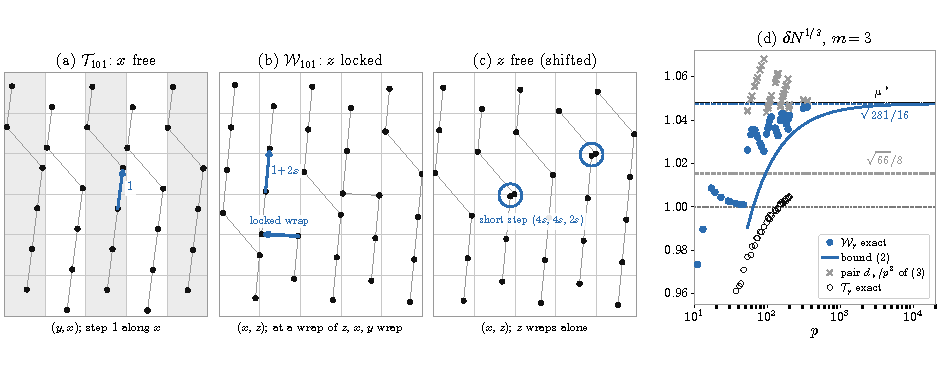
\includegraphics[width=\linewidth,height=0.5\textheight,keepaspectratio]{figs/w_net.pdf}}{\fbox{\parbox{0.9\textwidth}{\centering figure \texttt{w\_net} pending}}}
\caption{\wNetCaption\interactive{beyond.html}}
\label{fig:wnet}
\end{figure}

\emph{The balance.} In the limit the two shortest contacts are rows (a) and (b) of Table~\ref{tab:wcontacts}: the diagonal contact, lifted by the glue $\frac12+3\varepsilon$, and the step along $\e_z$, lengthened to $1+2\varepsilon$ in $z$. Their squared lengths
\[
q_a(\varepsilon)=\tfrac54-9\varepsilon+81\varepsilon^2,\qquad q_b(\varepsilon)=1+4\varepsilon+36\varepsilon^2
\]
are equal where $45\varepsilon^2-13\varepsilon+\frac14=0$. The smaller root is $\varepsilon^*=(13-2\sqrt{31})/90=0.02071\ldots$, and there both equal $\mu^{*2}$, where $\mu^*=\sqrt{(72-8\sqrt{31})/25}=1.0480\ldots$; on $[0,\frac1{18}]$, $q_a$ decreases and $q_b$ increases. The limit $\varepsilon=\frac1{48}=0.02083\ldots$ of $\mathcal W_p$ is not a balance: it lies just above $\varepsilon^*$, on the side of the diagonal contact, with $q_a(\frac1{48})=\frac{281}{256}<q_b(\frac1{48})=\frac{211}{192}$, and its length $\sqrt{281}/16$ is $0.030\,\%$ below $\mu^*$. Since $\rho$ is an integer, the drift $\varepsilon-\frac1{48}$ cannot vanish; the choice $\rho=2\lfloor p/48\rfloor+1$ centres it, $|\varepsilon-\frac1{48}|\le\frac{23}{48p}$, and it gives the first-order constant $\frac{345}{128}$ of (2). The balance $\mu^*$ is the optimum of the whole family of layers of this shape.

\begin{proposition}[Optimum of the rank-one layers with image $(2,2,1)$]\label{prop:wfamily}
Let $p\ge5$ be a prime, $\mathbf w=(2,2,1)$, and let $P$ be a digital $(0,3,3)$-net over $\F_p$ in graph form with the depths $(1,1,1)$ whose layer is $B=\mathbf w u^{\!\top}$ for some $u\in\F_p^3$, with any third rows: $z$ reads the second digit $\zeta(n)=u\cdot n\bmod p$, and $x$ and $y$ read $2\zeta(n)\bmod p$. For $\psi\in(\R/\Z)^3$ let $F(\psi)$ be the least value of $|E+\xi\mathbf w-\omega(1,1,0)|^2$ over the steps $E\in\Z^3\setminus\{0\}$ and the pairs $(\xi,\omega)$ with $\xi\in(-1,1)$, $\xi\equiv\psi\cdot E\pmod1$, and $\omega=\sgn\xi$, or $\omega=0$ if $|\xi|<\frac12$. Let $\psi^*=(\frac12-\varepsilon^*,\frac12-\varepsilon^*,2\varepsilon^*)$.
\begin{enumerate}
\item Let $F_p(u)$ be the squared toroidal minimum distance of the points $p^2n+p\,g(n)$ at integer scale $p^3$, divided by $p^4$, where $g(n)=(2\zeta(n)\bmod p,\,2\zeta(n)\bmod p,\,\zeta(n))$ are the second digits: the value of $(\delta N^{1/3})^2$ without the third digits. Then $F_p(u)=F(u/p)$, and $|\delta N^{1/3}-\sqrt{F_p(u)}|<\sqrt3/p$ for any third rows.
\item For $0<\varepsilon\le\frac3{100}$, $F(\frac12-\varepsilon,\frac12-\varepsilon,2\varepsilon)=\min(q_a(\varepsilon),q_b(\varepsilon))$.
\item $F(\psi)\le\mu^{*2}$ for every $\psi\in(\R/\Z)^3$, with equality only at $\psi=\psi^*$. As $\psi^*$ has irrational coordinates, $F_p(u)<\mu^{*2}$, and $\delta N^{1/3}<\mu^*+\sqrt3/p$.
\end{enumerate}
\end{proposition}

So no digital $(0,3,3)$-net whose layer has rank one with image $\F_p(2,2,1)$ exceeds $\mu^*+\sqrt3/p$, at any prime and with any third rows, and the supremum $\mu^{*2}$ of the value without the third digits is attained by no net. Permuting the coordinates gives the isometric families with the images $\F_p(2,1,2)$ and $\F_p(1,2,2)$.

\begin{proof}
Call a step $E$ with a pair $(\xi,\omega)$ as in the definition of $F$ an \emph{option} of $\psi$, with the vector $V=E+\xi\mathbf w-\omega(1,1,0)$. Every option has $|\xi|<1$ and $|2\xi-\omega|<1$, so $|V|>2$ if some $|E_c|\ge3$. The step $\e_z$ gives $V=\e_z$ if $\psi_z\equiv0$, and otherwise, with $\xi=\{\psi_z\}-1$ and $\omega=-1$, it gives $V=(2\xi+1,2\xi+1,1+\xi)$, whose entries lie in $(-1,1)$. Hence $F\le3$, and only the steps $E\in\{-2,\dots,2\}^3\setminus\{0\}$ matter.

(1) At integer scale $p^3$ the point of cell $n$ is $p^2n+p\,g(n)+f(n)$ with the third digits $f(n)$. As in the proof of Proposition~\ref{prop:wnet}(2), the representatives of the difference of the points of the cells $n$ and $n'$ are $D=p^2E+p\,\Delta g+\Delta f$ with $E\equiv n'-n\pmod p$ and $|\Delta f_c|<p$; without the third digits they are $p^2V$ with $V=E+\Delta g/p$, and $\bigl||D|/p^2-|V|\bigr|\le|\Delta f|/p^2<\sqrt3/p$. Comparing a pair that attains $\delta$ with one that attains $\sqrt{F_p(u)}$ gives $|\delta N^{1/3}-\sqrt{F_p(u)}|<\sqrt3/p$. By Lemma~\ref{lem:wwrap} (which holds for every $u$; part (1) uses neither $u\ne0$ nor the net property), $\Delta g=(2\Delta\zeta-p\omega,\,2\Delta\zeta-p\omega,\,\Delta\zeta)$, and the pairs $(\Delta\zeta,\omega)$ that occur for the step $E$ are those of the lemma. With $\xi=\Delta\zeta/p$ they are exactly the pairs of the definition of $F$ for $\psi=u/p$: $\Delta\zeta\in\{\sigma,\sigma-p\}$ (only $0$ if $\sigma=0$) means $\xi\in(-1,1)$ and $\xi\equiv u\cdot E/p\pmod1$, and, as $p$ is odd, $|\Delta\zeta|\le h$ means $|\xi|<\frac12$. Then $V=E+\xi\mathbf w-\omega(1,1,0)$. As $p\ge5$, every step $E\in\{-2,\dots,2\}^3\setminus\{0\}$ joins two distinct cells, so $F_p(u)=F(u/p)$.

(2) Let $\psi=(\frac12-\varepsilon,\frac12-\varepsilon,2\varepsilon)$ with $0<\varepsilon\le\frac3{100}$. With $S=E_x+E_y$ and $Q=S-2E_z$, $\psi\cdot E=\frac S2-Q\varepsilon$, so $\xi=\nu-Q\varepsilon$ with $\nu\in\frac S2+\Z$, and $V=A-Q\varepsilon\mathbf w$ with $A=E+(2\nu-\omega)(1,1,0)+\nu\e_z$. This is the parametrization of the proof of Proposition~\ref{prop:wnet}(2), where $u/p$ is of this form with $\varepsilon=\rho/(2p)$. As $|Q\varepsilon|\le8\varepsilon<\frac12$, the pairs that occur follow the rules stated there: for $\nu=0$, $|\xi|<\frac12$ and $\omega\in\{0,-\sgn Q\}$; for $\nu=\pm\frac12$, $\xi$ has the sign of $\nu$, $\omega=\sgn \nu$ occurs, and $\omega=0$ occurs if and only if $\nu Q>0$; $\nu=\pm1$ occurs only if $\nu Q>0$, and then $\omega=\sgn \nu$; and $|\nu|\ge\frac32$ does not occur. The rest of that proof uses only $\varepsilon\le\frac3{100}$: the options with $|A|^2\ge3$ have $|V|>1.05$, and the others are the rows of Table~\ref{tab:wcontacts}. On $(0,\frac3{100}]$ the rows (c), (d) and (f) decrease, to $1.1081$, $1.1681$ and $1.5524$, and the rows (e) and (g) are at least $\frac54$; all of these, and $1.05^2=1.1025$, exceed $\mu^{*2}$, while $\min(q_a(\varepsilon),q_b(\varepsilon))\le\mu^{*2}$, as $q_a$ decreases and $q_b$ increases through $\varepsilon^*$. The rows (a) and (b) occur, since $(\nu,\omega)=(\frac12,1)$ and $(0,0)$ are always allowed. So $F(\psi)=\min(q_a(\varepsilon),q_b(\varepsilon))$.

(3) Let $\psi\in(\R/\Z)^3$ with $F(\psi)\ge\mu^{*2}$, and represent $\psi_x,\psi_y,\psi_z$ by numbers in $[0,1)$. We use only options with $\omega=\sgn\xi$, which always occur, and options with $\omega=0$ and $|\xi|<\frac12$. The numbers $\frac{246}{225}=1.0933\ldots$, $\frac{17}{16}$ and $\frac9{25}$ are below $\mu^{*2}=1.0983\ldots$.

\emph{The step $\e_z$.} If $\psi_z=0$, then $V=\e_z$ and $|V|^2=1$. Otherwise $\xi=\psi_z-1$, $\omega=-1$ gives $V=(2\psi_z-1,2\psi_z-1,\psi_z)$ with $|V|^2=9\psi_z^2-8\psi_z+2$, a convex function with the values $\frac{246}{225}$ at $\psi_z=\frac2{15}$ and $\frac{17}{16}$ at $\psi_z=\frac34$; so $\psi_z\notin[\frac2{15},\frac34]$. If $\psi_z>\frac34$, then $\xi=\psi_z-1$, $\omega=0$ gives $|V|^2=8(1-\psi_z)^2+\psi_z^2\le\frac{17}{16}$. So $0<\psi_z<\frac2{15}$, and $\xi=\psi_z$, $\omega=0$ gives $V=(2\psi_z,2\psi_z,1+\psi_z)$ with $|V|^2=q_b(\psi_z/2)$; as $q_b$ increases, $\psi_z\ge2\varepsilon^*$.

\emph{The steps $\e_x$ and $\e_y$.} If $\psi_x=0$, then $|V|^2=1$. Otherwise $\xi=\psi_x$, $\omega=1$ gives $V=(2\psi_x,2\psi_x-1,\psi_x)$ with $|V|^2=9\psi_x^2-4\psi_x+1$, a convex function with the values $1$ at $\psi_x=0$ and $\frac{246}{225}$ at $\psi_x=\frac7{15}$; so $\psi_x>\frac7{15}$. If $\psi_x>\frac12$, then $\xi=\psi_x-1$, $\omega=0$ gives $V=(1-2t,-2t,-t)$ with $t=1-\psi_x$, and $|V|^2=9t^2-4t+1$ is the same function, so $t>\frac7{15}$. Hence $\alpha=\frac12-\psi_x\in(-\frac1{30},\frac1{30})$, and likewise $\beta=\frac12-\psi_y\in(-\frac1{30},\frac1{30})$. Put $\gamma=\psi_z$.

\emph{The step $\mathbf 1$ (the lock).} Here $\psi\cdot\mathbf 1\equiv\gamma-\alpha-\beta=:\tilde\sigma\in(-\frac1{15},\frac15)$. If $\tilde\sigma>0$, then $\xi=\tilde\sigma-1$, $\omega=-1$ gives $V=(2\tilde\sigma,2\tilde\sigma,\tilde\sigma)$ with $|V|^2=9\tilde\sigma^2<\frac9{25}$. So $\alpha+\beta\ge\gamma$.

\emph{The diagonal steps $(1,0,-1)$ and $(0,1,-1)$.} For $E=(1,0,-1)$, $\psi\cdot E\equiv\psi_x-\psi_z=\frac12-\lambda$ with $\lambda=\alpha+\gamma\in(2\varepsilon^*-\frac1{30},\frac16)\subset(0,\frac16)$, and $\xi=\frac12-\lambda$, $\omega=1$ gives $V=(1-2\lambda,-2\lambda,-\frac12-\lambda)$ with $|V|^2=\frac54-3\lambda+9\lambda^2=q_a(\lambda/3)$: row (a) of Table~\ref{tab:wcontacts} with $\varepsilon=\lambda/3$. Likewise $E=(0,1,-1)$ gives $q_a(\lambda'/3)$ with $\lambda'=\beta+\gamma$. As $q_a$ decreases on $[0,\frac1{18}]$ and $q_a(\varepsilon^*)=\mu^{*2}\le F(\psi)$, we get $\lambda\le3\varepsilon^*$ and $\lambda'\le3\varepsilon^*$. But $\lambda+\lambda'=\alpha+\beta+2\gamma\ge3\gamma\ge6\varepsilon^*$, by the lock and the step $\e_z$. So equality holds throughout: $\lambda=\lambda'=3\varepsilon^*$, $\alpha+\beta=\gamma$ and $\gamma=2\varepsilon^*$, hence $\alpha=\beta=\varepsilon^*$, i.e.\ $\psi=\psi^*$.

Hence $F(\psi)\ge\mu^{*2}$ only at $\psi=\psi^*$, where $F(\psi^*)=\mu^{*2}$ by (2): $F\le\mu^{*2}$ everywhere, with equality only at $\psi^*$. As $\varepsilon^*$ is irrational, $u/p\ne\psi^*$, so $F_p(u)=F(u/p)<\mu^{*2}$, and by (1) $\delta N^{1/3}<\sqrt{F_p(u)}+\sqrt3/p<\mu^*+\sqrt3/p$.
\end{proof}

\emph{How six contacts fix the optimum.} The proof uses six steps. Along $\e_x$, $\e_y$ and $\e_z$ a coordinate can wrap alone, which shortens the step. This forces $\psi_x$ and $\psi_y$ to stay within $\frac1{30}$ of $\frac12$ ($|\alpha|,|\beta|<\frac1{30}$), and $z$ to move by at least $1+2\varepsilon^*$ along $\e_z$ ($\gamma\ge2\varepsilon^*$), or the step along $\e_z$ is short. The step $\mathbf 1$ is the one along which all three coordinates can wrap together, and these offsets must not shorten it: $\alpha+\beta\ge\gamma$. The diagonal contacts then balance against the step along $\e_z$, at an irrational point. The optimum lies on the plane $\psi\cdot\mathbf 1\equiv0$, i.e.\ $u\cdot\mathbf 1\equiv0$, where the step $\mathbf 1$ has no phase change; $\mathcal W_p$ lies on it, as $2(h-r)+\rho=p$. Proposition~\ref{prop:wfamily} covers only the image $\F_p(2,2,1)$ and its permutations; other rank-one images, layers of rank two and non-digital point sets are not covered (Remark~\ref{rem:open}(7)).

\begin{remark}[Reaching $\mu^*$]\label{rem:wstar}
Let $\mathcal W^*_p$ be the net of Proposition~\ref{prop:wnet} with $r=\lfloor p\varepsilon^*\rfloor$ in place of $\lfloor p/48\rfloor$. Then $\rho=2r+1$ is the odd integer nearest to $2p\varepsilon^*$, and $\varepsilon_p=\rho/(2p)$ satisfies $|\varepsilon_p-\varepsilon^*|<\frac1{2p}$ (both use that $p\varepsilon^*$ is never an integer, as $\varepsilon^*$ is irrational). $\mathcal W^*_p$ is a $(0,3,3)$-net for every prime $p\ge5$, since the proof of Proposition~\ref{prop:wnet}(1) needs only $1\le\rho<p$ and $1\le h-r<p$. Its layer is $\mathbf w u^{\!\top}$ with $u/p=(\frac12-\varepsilon_p,\frac12-\varepsilon_p,2\varepsilon_p)$, and $\varepsilon_p\le\frac3{100}$ for $p\ge17$ ($\varepsilon_p=\frac1{2p}$ for $p\le47$, $\varepsilon_{53}=\frac3{106}$, and $\varepsilon^*+\frac1{118}<\frac3{100}$). So for $p\ge17$ Proposition~\ref{prop:wfamily}(1), (2) gives the value $\min(q_a(\varepsilon_p),q_b(\varepsilon_p))$ without the third digits. Both $q_a$ and $q_b$ are convex, so each lies above its tangent line at $\varepsilon^*$; there $q_a$ decreases and $q_b$ increases, and $q_b'(\varepsilon^*)<|q_a'(\varepsilon^*)|$; hence
\[
\delta N^{1/3}(\mathcal W^*_p)\ >\ \sqrt{\mu^{*2}-\frac Kp}-\frac{\sqrt3}p,\qquad K=\frac{|q_a'(\varepsilon^*)|}2=\frac{9\sqrt{31}-36}5=2.8219\ldots,
\]
for every prime $p\ge17$. With Proposition~\ref{prop:wfamily}(3), $\delta N^{1/3}(\mathcal W^*_p)\to\mu^*$: the optimum of the family is attained in the limit. The bound exceeds $1$ from $p=67$ on and $\sqrt{66}/8$ from $p=97$ on, as that of Proposition~\ref{prop:wnet}(2). It exceeds $\sqrt{281}/16$ from $p=9791$ on, and the upper bound $\sqrt{281}/16+5/(2p)$ of Proposition~\ref{prop:wnet}(3) from $p=17737$ on; only from there on is $\mathcal W^*_p$ provably ahead of $\mathcal W_p$.

The optimum is reached only asymptotically: at moderate $p$, $\mathcal W^*_p$ is not ahead of $\mathcal W_p$. $\mathcal W^*_p=\mathcal W_p$ for $p<193$ (computed), and $\mathcal W^*_p\ne\mathcal W_p$ for $p>8548$: as $\frac1{48}-\varepsilon^*=\frac{96\sqrt{31}-534}{4320}>\frac1{8549}$, for $p\ge8549$ we have $p/48-p\varepsilon^*>1$, so $\lfloor p/48\rfloor>\lfloor p\varepsilon^*\rfloor$, and the two nets have different $\rho<p$. At the primes $p\le1009$ where they differ, namely $193$, $241$, $337$, $433$, $577$, $673$, $769$ and $1009$, $\mathcal W_p$ has the larger $\delta N^{1/3}$ (computed; $1.0405\ldots$ against $1.0355\ldots$ at $p=193$, and $1.0463\ldots$ against $1.0458\ldots$ at $p=1009$). At these primes $\varepsilon_p<\varepsilon^*$ for $\mathcal W^*_p$, so without the third digits its minimum is the step (b) along $\e_z$, while $\mathcal W_p$ has $\varepsilon>\varepsilon^*$ and its minimum is the diagonal contact (a). A heuristic reading of the computed values is that the third rows of Proposition~\ref{prop:wnet} cost the step (b) more than the contact (a): at moderate $p$ the jitter, not the drift, decides, and the value that $\mathcal W_p$ gives up by its limit $\varepsilon\to\frac1{48}$ instead of $\varepsilon^*$ is small, $\mu^{*2}-\frac{281}{256}<7\cdot10^{-4}$.
\end{remark}

\emph{Computed values.} The exact $\delta N^{1/3}$ of $\mathcal W_p$ is $1.0087\ldots$ at $p=17$, $1.0262\ldots$ at $p=53$, $1.0362\ldots$ at $p=101$ and $1.0461\ldots$ at $p=353$, and below $1$ for $p\le13$ (computed). By (4) and Corollary~\ref{cor:colceil}, $\mathcal W_p$ is ahead of every column point set at every prime $p\ge17$. It is ahead of $\mathcal T_p$ at every prime $17\le p\le199$ other than $23$ (computed), and for $p\ge53$ also by (4) and Proposition~\ref{prop:twocoset}(3), as $\delta(\mathcal T_p)N^{1/3}\le d_*(\mathcal T_p)/p^2<\sqrt{66}/8$. Nor is $\sqrt{66}/8$ the best value for layers in which two coordinates share a geometric digit: in the limit model the layer $A=\frac1{15}\left(\begin{smallmatrix}0&6&6\\2&-1&-1\\2&-1&-1\end{smallmatrix}\right)$ with $Y=\{\psi\in(\R/\Z)^3:\psi_y=\psi_z\}$ has the value $\sqrt{233}/15=1.0176\ldots$ (computed), and its realization $B_x=(0,a,a)$, $B_y=B_z=(2r',-r',-r')$, $a=\operatorname{round}(2p/5)$, $r'=\operatorname{round}(p/15)$, with the third rows of $\mathcal T_p$, is a $(0,3,3)$-net at $p=307$ with $\delta N^{1/3}=1.0160\ldots>\sqrt{66}/8$ (computed). Its free coordinate $x$ carries the glue $\frac25$. So Remark~\ref{rem:glue}, which concerns the length of a single step under free wraps, does not decide which glue is optimal for the minimum, even for free coordinates.

\emph{Only at $m=3$.} At $m=3k$, $k\ge2$, the geometric digits of any two coordinates of a $(0,m,3)$-net are jointly uniformly distributed (Lemma~\ref{lem:shared}), so no coordinate can read half, or any function, of the geometric digit of another: the lock of $\mathcal W_p$, like that of $\mathcal T_p$, exists only at $m=3$ (Remark~\ref{rem:open}(7)).

\begin{remark}[Digital shifts of $\mathcal T_p$ and $\mathcal W_p$]\label{rem:wshift}
As for the column nets (Remark~\ref{rem:shiftshared}), a digital shift translates the wrap windows of the coordinates independently, so bounds that use locked wraps need not survive it. The bound of Proposition~\ref{prop:twocoset}(2) does not extend to shifts whose second digits differ in $y$ and $z$, the two coordinates that share their geometric digit, for instance at $p=41$, $53$, $101$ (computed). If they agree, $\tau_{y,2}=\tau_{z,2}$ (all other shift digits arbitrary), the bound holds for the shifted net, for every prime $p\ge41$. Indeed, by Lemma~\ref{lem:shift} the shifted net, indexed by its own cells, is $\mathcal T_p$ with constants added to the offset digits. As $C_y$ and $C_z$ have the same second row, the geometric digits of $y$ and $z$ of each cell differ by the constant $\tau_{y,2}-\tau_{z,2}=0$, so $g_y=g_z$ at every cell; and the differences of the geometric digits of two cells satisfy the same congruences $\xi\equiv hS$, $\eta\equiv rE_x-T$ as for $\mathcal T_p$, since the constants cancel. The proof of Proposition~\ref{prop:twocoset}(2) uses the geometric digits only through these congruences and through $g_y=g_z$, and the third digits only through $|\Delta f_c|<p$; so it applies verbatim. The lock of $\mathcal W_p$ (Proposition~\ref{prop:wnet}) is more fragile, because $z$ reads half of the digit of $x$ and $y$. In the notation of Lemma~\ref{lem:wwrap} ($z$ reads $\zeta(n)=u\cdot n\bmod p$, and $x$ and $y$ read $2\zeta(n)\bmod p$), let the second shift digits be $\tau_{x,2}=\tau_{y,2}=t$ and $\tau_{z,2}=t'$. Re-indexing the cells by $n'=n+n_0$, for a cell $n_0$ with $u\cdot n_0\equiv t'$ (a translation of the torus by $-n_0$ cells, together with a shift of the third digits), turns the shifted net into the one in which $z$ reads $\zeta(n)$ and $x$ and $y$ read $(2\zeta(n)+t-2t')\bmod p$. For $t\equiv2t'$ this is $\mathcal W_p$ with shifted third digits. For $t\equiv2t'+1$ the digit $(2\zeta+1)\bmod p$ wraps, i.e.\ $2\zeta+1\ge p$, if and only if $\zeta\ge h$, one step earlier than $2\zeta$, and with $\omega=[2\zeta(n')+1\ge p]-[2\zeta(n)+1\ge p]$ the pairs $(\Delta\zeta,\omega)$ that occur are exactly those of Lemma~\ref{lem:wwrap}. Indeed, the proof of the lemma goes through with $h$ in place of $h+1$: the values of $\Delta\zeta$ and the reversal are unchanged, and for $\Delta\zeta=d>0$ and $\zeta=\zeta(n)\in[0,p-1-d]$ we have $\omega\in\{0,1\}$; $\omega=1$ if and only if $\zeta\le h-1<\zeta+d$, which holds for $\zeta=\max(0,h-d)$, so it occurs for every $d$; and $\omega=0$ if and only if $\zeta+d\le h-1$, possible if and only if $d\le h-1$ (both digits below the wrap), or $\zeta\ge h$, possible if and only if $h\le p-1-d$, i.e.\ $d\le h$ (both at or above it). So $\omega=0$ occurs if and only if $d\le h$, as in the lemma. The proof of Proposition~\ref{prop:wnet}(2) uses the second digits only through these pairs and allows any third digits, so its bound holds for the shifted net whenever $t\equiv2t'$ or $t\equiv2t'+1$; the exact value need not be kept, since the third digits move. Other second digits break the lock in every case computed: at $p=101$ the shifts $(\tau_{x,2},\tau_{y,2},\tau_{z,2})=(0,0,1)$ and $(7,7,7)$ give $\delta N^{1/3}=.1355\ldots$, against $1.0362\ldots$ without a shift, and every shift $(t,t,0)$ with $2\le t\le100$ gives $\delta N^{1/3}<0.1356$, while $(1,1,0)$, $(3,3,1)$ and $(5,5,2)$ keep $1.0362\ldots$ (computed). That only $t\equiv2t'$ and $t\equiv2t'+1$ keep the lock is computed, not proved. In the computed cases where the lock breaks, the step along $\e_z$ at a wrap of $z$ alone shrinks to $(4\varepsilon,4\varepsilon,2\varepsilon)$ up to the third digits. Proposition~\ref{prop:wnet} is a statement about unshifted nets.
\end{remark}

\subsection{No half-integer layer in the frame orbit}\label{sec:Pnohalf}
By Section~\ref{sec:frames}, every net obtained from a frame by per-coordinate lower-triangular scrambles has a geometric layer of Cauchy form, $\tilde M_{cd}=\lambda_c\mu_d/D_{cd}$ ($c\ne d$), with units $\lambda_c,\mu_d$ and the homogeneous place differences $D_{cd}$; this holds over $\mathbb{Q}$, and verbatim over $\F_p$ for places in $\mathbb P^1(\F_p)$. The deepest carry depth $s-2$ of row~$0$ is free by Proposition~\ref{prop:F} up to one condition per column $d$ (the polynomial $g_{d,s-2}$ there, which the $s-1$ off-diagonal entries of the column determine, must have a unit leading coefficient) and can be made half-integer. But the geometric layer $F_0$, which every carry-free step sees, sits at carry depth $0$, where the Cauchy form leaves only the row and column scalars free.

\begin{proposition}[No half-integer frame layer]\label{prop:P}
Let $\tilde M$ be a layer of this Cauchy form over a field $\mathbb K$, and let $a,b,c,d$ be four distinct coordinates.
\begin{enumerate}
\item If $\mathbb K=\F_p$, $p$ prime, and $2\tilde M_{ij}\equiv h_{ij}\pmod p$ for all twelve ordered pairs $i\ne j$ in $\{a,b,c,d\}$, with odd integers $|h_{ij}|\le\Omega$, then $p$ divides a nonzero odd integer $Z$ with $|Z|\le13\Omega^{16}$. In particular this is impossible for $p>13\Omega^{16}$.
\item If $\mathbb K=\mathbb{Q}$, then the twelve entries $\tilde M_{ij}$, $i\ne j$ in $\{a,b,c,d\}$, do not all lie in $\frac12+\Z$.
\end{enumerate}
\end{proposition}

\begin{proof}
By Lemma~\ref{lem:CH}(P) over $\mathbb K$, with $\pi_{ij}=\tilde M_{ij}\tilde M_{ji}$, the numbers $\chi^2=\pi_{ab}\pi_{cd}/(\pi_{ac}\pi_{bd})$ and $\psi^2=\pi_{ab}\pi_{cd}/(\pi_{ad}\pi_{bc})$ satisfy $(\chi^2-\psi^2-1)^2=4\psi^2$.
(1) The entries of a layer of Cauchy form are units, so for odd $p$ the $h_{ij}\equiv2\tilde M_{ij}$ are units modulo $p$ (for $p=2$ the hypothesis fails, the $h_{ij}$ being odd), and $4\pi_{ij}\equiv h_{ij}h_{ji}$. Let $A_1=|h_{ab}h_{ba}h_{cd}h_{dc}|$, $A_2=|h_{ac}h_{ca}h_{bd}h_{db}|$, $A_3=|h_{ad}h_{da}h_{bc}h_{cb}|$, odd integers at most $\Omega^4$. Then $\chi^2\equiv\varepsilon_2A_1/A_2$ and $\psi^2\equiv\varepsilon_3A_1/A_3$ with signs $\varepsilon_2,\varepsilon_3\in\{\pm1\}$, and multiplying the last relation by $A_2^2A_3^2$ shows that $p$ divides
\[
Z=\bigl(\varepsilon_2A_1A_3-\varepsilon_3A_1A_2-A_2A_3\bigr)^2-4\varepsilon_3A_1A_2^2A_3 .
\]
The bracket is a sum of three odd numbers, hence odd, so $Z$ is odd and in particular nonzero, and $|Z|\le(3\Omega^8)^2+4\Omega^{16}=13\Omega^{16}$.
(2) Over $\mathbb{Q}$ the same computation with $h_{ij}=2\tilde M_{ij}$, odd integers by assumption, gives $Z=0$ exactly, contradicting that $Z$ is odd.
\end{proof}

So a rational design never has a half-integer geometric layer in the frame orbit (on four coordinates, hence for $s\ge4$), and a design over $\F_p$ with $|2\tilde M|\le\Omega$ has none once $p>13\Omega^{16}$. Proposition~\ref{prop:P} reads the Pl\"ucker relation of Lemma~\ref{lem:CH}(P) modulo powers of $2$: it is the $2$-adic counterpart of Lemma~\ref{lem:CH}(H), which reads it in absolute value, and of Remark~\ref{rem:pm1}, which reads it modulo $q$.

\subsection{The split frame}\label{sec:split}
The ceilings of Theorems~\ref{thm:L} and~\ref{thm:O5} concern bounded layers. A geometric layer with half-integer entries escapes them: locally the points form the packing $D_s^+=D_s\cup(D_s+\frac12\mathbf 1)$ \cite[Ch.~4]{CS99}, whose minimum $\min(\sqrt s/2,\sqrt2)$ exceeds $1$ for $s\ge5$ and equals the $E_8$ value $\sqrt2$ at $s=8$. At the resolution $m=s$ no frame is needed (Section~\ref{sec:halfms}). For $k\ge2$ the layer sits at carry depth $0$ of a design, and there a Pl\"ucker relation between the places excludes rational half-integer layers in the frame orbit (Proposition~\ref{prop:P}). To escape it, the split frame lets each coordinate $c$ read its cell digits at one point $v_c$ and its offset digits at a different point $u_c$. Its box minors are still confluent Vandermonde determinants, its geometric layer is the non-symmetric Cauchy matrix $\lambda'_c\mu_d/(u_c-v_d)$ in two unrelated point sets, and with $u_c$ even and $v_d$ odd it can be half-integer at every carry depth.

\begin{definition}\label{def:split}
Let $v_0,\dots,v_{s-1}$ (\emph{cell points}) and $u_0,\dots,u_{s-1}$ (\emph{offset points}) be $2s$ pairwise distinct rational numbers, let $D$ be the product of their denominators and of the numerators of their pairwise differences, $R=\Z[1/D]$ and $m=sk$. For $V\in R[t]_{<m}$ let coordinate $c$ have the $m$ digits
\[
[(t-v_c)^j]\,V\quad(j<k),\qquad\text{followed by}\qquad[(t-u_c)^j]\,V\quad(j<m-k).
\]
Put $\vartheta_{cd}=u_c-v_d$, $\Pi(t)=\prod_d(t-v_d)^k$, $\Pi_d=\Pi/(t-v_d)^k$ and $\Theta_c=\prod_{d}\vartheta_{cd}$, so that $\Pi(u_c)=\Theta_c^k$.
\end{definition}

With $u=v$ (and one place at $\infty$) this would be the frame of Section~\ref{sec:dim4}. Here the cell of coordinate $c$ is the $k$-jet of $V$ at $v_c$ and its offset is the jet at a different point $u_c$ (Figure~\ref{fig:arcsplit}).

\begin{figure}[tbp]
\centering
\arcfig{arc_split}
\caption{\arcSplitCaption}
\label{fig:arcsplit}
\end{figure}

\begin{lemma}[Box minors of the split frame]\label{lem:Tsplit}
For depths $(d_c)$ with $\sum_cd_c=m$ the box matrix of the split frame consists of the $\min(d_c,k)$-jets of $V$ at $v_c$ and the $(d_c-k)_+$-jets at $u_c$, and its determinant is, up to sign, the confluent Vandermonde product $\prod_{\{P,Q\}}(x_Q-x_P)^{\alpha_P\alpha_Q}$ over the $2s$ points $x_P$ with these multiplicities $\alpha_P$. In particular, for $s\ge4$, every $k\ge1$ and $q$ coprime to the denominators of the points, the split frame is a $(0,sk,s)$-net over $\Z/q\Z$ if and only if the $2s$ points are pairwise distinct modulo every prime factor of $q$ (which needs every prime factor of $q$ to be at least $2s$).
\end{lemma}

\begin{proof}
The box matrix is the Hermite matrix of Lemma~\ref{lem:hermite} for the $2s$ points with the multiplicities $\alpha_P$, $\sum_P\alpha_P=\sum_cd_c=m$ (no point at $\infty$); this gives the value, a unit modulo $p$ if the points are distinct modulo $p$. Conversely, a coincidence modulo $p$ puts two equal rows into some box: $V(v_c)$ and $V(v_d)$ for $v_c\equiv v_d$ (the box $(k,\dots,k)$); $V(u_c)$ and $V(v_d)$ for $u_c\equiv v_d$, $c=d$ allowed (depth $k+1$ on $c$, at least $1$ on $d$); $V(u_c)$ and $V(u_d)$ for $u_c\equiv u_d$, $c\ne d$ (depths $k+1$ on $c$ and $d$, $k-1$ on two other coordinates, $k$ elsewhere; here $s\ge4$ is used). Then Lemma~\ref{lem:nie}.
\end{proof}

So the $t=0$ property of split frames is Lemma~\ref{lem:hermite} with two points per coordinate (the exact sign is recorded in Appendix~\ref{app:formal}). As for frames, the $(k,\dots,k)$ box is invertible over $R$, so the split frame has a graph form $\Phi^S$ with depths $(k,\dots,k)$ and entries in $R$, whose box minors are those of Lemma~\ref{lem:Tsplit} divided by the unit $(k,\dots,k)$ minor.

\begin{lemma}[First offset rows of the split frame]\label{lem:Rsplit}
For every $k\ge1$ and $c\ne d$, row $0$ of $\Phi^S_{cd}$ has, with $x^n$ marking carry depth $n$, the generating function
\[
\frac{\Theta_c^k}{\Pi_d(v_d+x)\,(\vartheta_{cd}-x)}.
\]
\end{lemma}

\begin{proof}
As $\deg V<sk=\deg\Pi$, partial fractions give $V=\sum_d\Pi_dN_d$ with $\deg N_d<k$; as $V\equiv\Pi_dN_d\pmod{(t-v_d)^k}$ and $\Pi_d(v_d)$ is a unit, the cell of $d$ determines $N_d$ and conversely. The first offset digit of $c$ is $V(u_c)$. For the column (level $j$ of the cell of $d$, all other cells $0$) we have $V=\Pi_dN_d$ with $N_d\equiv(t-v_d)^j/\Pi_d\pmod{(t-v_d)^k}$, i.e. $N_d=\sum_{j\le i<k}\varphi_{i-j}(t-v_d)^i$ with $\varphi(x)=\sum_n\varphi_nx^n=1/\Pi_d(v_d+x)$. Hence, with $\vartheta=\vartheta_{cd}$, $V(u_c)=\Pi_d(u_c)\sum_{j\le i<k}\varphi_{i-j}\vartheta^i$. Weighting the level $j=k-1-n$ by $x^n$ gives $\Pi_d(u_c)\,\vartheta^{k-1}\varphi(x)\sum_{r\ge0}(x/\vartheta)^r=\Pi_d(u_c)\vartheta^k\varphi(x)/(\vartheta-x)$ modulo $x^k$, and $\Pi_d(u_c)\vartheta^k=\Pi(u_c)=\Theta_c^k$.
\end{proof}

\begin{proposition}[Normal form and reachable designs of the split frame]\label{prop:Gsplit}
Apply the gauge move of Lemma~\ref{lem:box}(c) with $L_c=\operatorname{diag}(\Theta_c^{-k},1,\dots,1)$ and $U_d=\operatorname{Toep}(\Pi_d(v_d+x))$. Then row $0$ of every off-diagonal block becomes $w_{cd}/(1-y_{cd}x)$ with
\[
w_{cd}=y_{cd}=\frac1{\vartheta_{cd}}=\frac1{u_c-v_d}\qquad(c\ne d),
\]
independently of $k$, and within each column $d$ the $y_{cd}$ ($c\ne d$) are pairwise distinct with unit differences $y_{cd}-y_{c'd}=(u_{c'}-u_c)/(\vartheta_{cd}\vartheta_{c'd})$. Consequently Propositions~\ref{prop:Gs} and~\ref{prop:F}, Definition~\ref{def:Ns} and Corollary~\ref{cor:tsk} hold verbatim for the split frame, with $Q_c$ replaced by $\Theta_c$ and Lemma~\ref{lem:Ts} by Lemma~\ref{lem:Tsplit}. In particular a design is reachable with row scalars $\lambda'$ if and only if, for every column $d$ and every $j\le s-2$,
\[
M^{(j)}[c][d]=\lambda'_c\,\frac{g_{d,j}(y_{cd})}{u_c-v_d}\qquad(c\ne d)
\]
for polynomials $g_{d,j}$ of degree $j$ with unit leading coefficient; and then, for every $k\ge1$ and every $q$ coprime to $DD'$, where $D'$ collects the primes of the units $\lambda'_c$, of the leading coefficients of the $g_{d,j}$ and of the denominators, the graph form $\mathcal P^{u,v,F}_{k,q}$ of Definition~\ref{def:Ns} (on the split frame) is a digital $(0,sk,s)$-net over $\Z/q\Z$ with one point in every cell, whose row $0$ equals the design on the levels $k-1,\dots,k-\min(k,s-1)$ and vanishes below.
\end{proposition}

\begin{proof}
The normal form is Lemma~\ref{lem:Rsplit} times $\Theta_c^{-k}$ and $\Pi_d(v_d+x)$, as in Proposition~\ref{prop:Ns}, with unit diagonal entries of $L_c$ and $U_d$. The proofs of Propositions~\ref{prop:Gs} and~\ref{prop:F} use only that the $w_{cd}$ are units and that the $y_{cd}$ of a column are distinct with unit differences (the matrix $(w_{cd}y_{cd}^n)_{c\ne d,\,n\le s-2}$ is then a unit diagonal times an invertible Vandermonde matrix), and the proof of Corollary~\ref{cor:tsk} uses only the unit box minors of the frame, here Lemma~\ref{lem:Tsplit}.
\end{proof}

Only the leading coefficients of the $g_{d,j}$ with $j<\min(k,s-1)$ enter at a given $k$; if a prime $p$ divides the leading coefficient of some $g_{d,j}$, the design cannot be realized modulo $p$ at carry depth $j$, so modulo $p$ the net exists only for $k\le j$ (this is also verified in Lean). The geometric layer is now $M^{(0)}_{cd}=\lambda'_c\mu_d/(u_c-v_d)$ with $\mu_d=g_{d,0}$: a general, non-symmetric Cauchy matrix in two different sets of points. There is no Pl\"ucker relation between the row points $u_c$ and the column points $v_d$, so Proposition~\ref{prop:P} does not apply, and parities can be prescribed.

\begin{lemma}[Half-integer designs]\label{lem:Hs}
Let the $u_c$ be even and the $v_d$ odd integers, so that every $\vartheta_{cd}=u_c-v_d$ is odd, put $\Lambda_c=\prod_{d\ne c}\vartheta_{cd}^{\,s-1}$, and take $\lambda'_c=\frac12\Lambda_c$, $g_{d,0}=1$ and $g_{d,j}(y)=1+2y^j$ for $1\le j\le s-2$. Then
\[
M^{(0)}[c][d]=\frac{\Lambda_c}{2\vartheta_{cd}},\qquad M^{(j)}[c][d]=\frac{\Lambda_c}{2\vartheta_{cd}}+\frac{\Lambda_c}{\vartheta_{cd}^{\,j+1}}\quad(1\le j\le s-2),
\]
all in $\frac12+\Z$ ($c\ne d$),
so the off-diagonal part of $F_0$ lies in $\frac12+\Z$ and $F_j=M^{(j)}-M^{(j-1)}$ is an integer matrix for $j\ge1$. Complete the design by $F_0[c][c]=-\alpha_c$, with $\alpha_c$ the least element of $\frac12+\Z$ that is at least $A_c=\sum_{d\ne c}\max_{j\le s-2}|M^{(j)}[c][d]|$, and $F_j[c][c]=0$ for $j\ge1$. The primes of $DD'$ are $2$ and the primes of the point differences and of the $\Lambda_c$. For $u_c=2c$, $v_d=2d+1$ they are all at most $2s-1$.
\end{lemma}

We write $H_s$ for the design of Lemma~\ref{lem:Hs} with $u_c=2c$, $v_d=2d+1$.

\begin{proof}
By Proposition~\ref{prop:Gsplit}, $M^{(0)}[c][d]=\frac12\Lambda_c\vartheta_{cd}^{-1}$ and $M^{(j)}[c][d]=\frac12\Lambda_c\vartheta_{cd}^{-1}(1+2\vartheta_{cd}^{-j})$ for $1\le j\le s-2$. For $1\le i\le s-1$, $\Lambda_c/\vartheta_{cd}^{\,i}$ is a product of odd integers, hence an odd integer; so the first term lies in $\frac12+\Z$ and the second in $\Z$. The leading coefficients are $1$ and $2$, and $\mu_d=1$. For $H_s$ the differences $u_c-u_{c'}$, $v_d-v_{d'}$ and $\vartheta_{cd}=2(c-d)-1$ have absolute value at most $2s-1$.
\end{proof}

\subsection{Separation with carries}
For a design with half-integer $F_0$, every partial sum $M^{(j)}$ lies in $\frac12+\Z$, and this parity is all that the separation argument needs, at every carry pattern. As in Lemma~\ref{lem:Ss}, we bound each coordinate by the smallest of the possible changes of its geometric digit (its \emph{options}); all numbers below use this form.

\begin{proposition}[Half-integer layers with carries]\label{prop:Hk}
Let $p$ be an odd prime, $s\ge3$, $k\ge1$, $L=\min(k,s-1)$, and let a graph form over $\F_p$ be given (a digital net or not; no part uses $t=0$) with depths $(k,\dots,k)$ whose row $0$ of every block, diagonal included, equals a design $(F_0,\dots,F_{L-1})$ on the levels $k-1,\dots,k-L$ and vanishes below (the rows $\ge1$ are arbitrary). Assume
\[
\text{(Half)}\qquad F_0\in(\tfrac12+\Z)^{s\times s},\qquad F_i\in\Z^{s\times s}\ (1\le i\le L-1),
\]
with $\frac12\equiv(p+1)/2$. For $0\ne E\in\{-2,\dots,2\}^s$ (steps of two cells are included, because an offset change of about $\pm\frac p2$ can bring the points of cells two apart to about $1.5$ cells apart, below the cap $2$ of $\mathrm{LB}$) and carry depths $j_d\in\{0,\dots,L-1\}$ on the moving axes put $\Sigma E=\sum_cE_c$,
\[
\sigma_c=\sum_{d:\,E_d\ne0}\Bigl(E_dF_0[c][d]+\sgn(E_d)\sum_{i=1}^{j_d}F_i[c][d]\Bigr)
\]
(so $\sigma_c=\sum_dE_dM^{(j_d)}[c][d]$ if $|E|_\infty\le1$), let the \emph{options} of coordinate $c$ be $O_c=\{\sigma_c+\frac p2,\sigma_c-\frac p2\}$ if $\Sigma E$ is odd, $O_c=\{\sigma_c,\sigma_c-p\sgn\sigma_c\}$ if $\Sigma E$ is even ($O_c=\{0\}$ if $\sigma_c=0$), $b_c=\min_{t\in O_c}\max(0,|pE_c+t|-1)$, and $\mathrm{LB}=\min\bigl(2,\min_{E,j}|b|/p\bigr)$.
\begin{enumerate}
\item If $p>2\max|\sigma_c|$ (over all $E$, $j$ and $c$), then $\delta N^{1/s}\ge\mathrm{LB}$ (toroidal distance), for every choice of the rows $\ge1$.
\item Suppose moreover that $F_i[c][c]=0$ for $i\ge1$ and $F_0[c][c]=-\alpha_c$ with
\[
\alpha_c\ \ge\ A_c:=\sum_{d\ne c}\max_{j<L}\bigl|M^{(j)}[c][d]\bigr|.
\]
Let $B=\max_c(2\alpha_c+2A_c)$ (the dominance constant) and $\epsilon_p=(B+1)/p$. If $p>2B$, then $\delta N^{1/s}\ge\min\bigl(\sqrt s(\frac12-\epsilon_p),\sqrt2(1-\epsilon_p)\bigr)$.
\item Let $C=\max_{c,d}|F_0[c][d]|$. If $p>4sC+2$, then $\delta N^{1/s}\le\min(\sqrt s/2,\sqrt2)+\sqrt s\,(2C+1)/p$.
\end{enumerate}
\end{proposition}

\begin{proof}
(1) In cell units, coordinate $c$ of the point of cell $n$ is $n_c+(r_c+f_c)/p$ with $r_c$ the first offset digit and $f_c\in[0,1)$. Let $n\ne n'$ and let $E$ be a torus representative of $n'-n$ (modulo $p^k$ in each coordinate). If some $|E_c|\ge3$, then the two points differ by $|D_c|>|E_c|-1\ge2$ cells in coordinate $c$, with $D$ their difference in cell units, since $(r'_c+f'_c)-(r_c+f_c)\in(-p,p)$. Otherwise adding $E_d$ to the cell integer $n_d$ changes its level $k-1$ by $E_d$ and the levels $k-1-i$, $1\le i\le j_d$, by $\sgn(E_d)$ (carries or borrows; a carry is at most $1$ since $|E_d|\le2<p$, and the torus wrap is the full carry); since row $0$ vanishes below level $k-L$, capping $j_d$ at $L-1$ is exact. So $\Delta r_c=r'_c-r_c\equiv\sigma_c\pmod p$ with $\Delta r_c\in(-p,p)$. As $F_0\in(\frac12+\Z)^{s\times s}$ and $F_i$ is integral, $\sigma_c\in\Sigma E/2+\Z$. If $\Sigma E$ is odd, $\sigma_c\pm\frac p2$ are the integers congruent to $\sigma_c$ (with $\frac12\equiv(p+1)/2$), and as $|\sigma_c|<p/2$ they are the only ones in $(-p,p)$; if $\Sigma E$ is even, $\sigma_c$ is an integer with $|\sigma_c|<p$, and the integers in $(-p,p)$ congruent to it are $\sigma_c$ and $\sigma_c-p\sgn\sigma_c$ (only $0$ if $\sigma_c=0$). So $\Delta r_c\in O_c$, and $p|D_c|=|pE_c+\Delta r_c+\Delta f_c|>|pE_c+\Delta r_c|-1$, i.e. $p|D_c|\ge b_c$.

(2) First $|\sigma_c|\le2\alpha_c+2A_c\le B$, since the own term is $-E_c\alpha_c$ and the term of an axis $d\ne c$ is $E_dM^{(j_d)}[c][d]$ ($|E_d|=1$) or $\sgn(E_d)(M^{(0)}+M^{(j_d)})[c][d]$ ($|E_d|=2$); so (1) applies. Let $e=|E|_\infty\le2$ and $|E_c|=e$. Then $E_c\sigma_c\le-e^2\alpha_c+e\cdot eA_c\le0$: every coordinate of maximal size is backward. If $\Sigma E$ is odd, every coordinate has $|pE_c+t|\ge p|E_c\pm\frac12|-|\sigma_c|\ge p/2-|\sigma_c|$ for $t\in O_c$, so $|D_c|\ge\frac12-\epsilon_p$ for all $s$ coordinates. If $\Sigma E$ is even, a backward coordinate $c$ with $|E_c|=e$ has $\sgn\sigma_c\ne\sgn E_c$, so both options give $|pE_c+t|\ge pe-|\sigma_c|$ and $|D_c|\ge e-\epsilon_p$. For $e=2$ this is at least $2-\epsilon_p\ge\sqrt2(1-\epsilon_p)$; for $e=1$ an even $\Sigma E$ needs at least two nonzero coordinates, each of maximal size, so $|D|\ge\sqrt2(1-\epsilon_p)$.

(3) Since $|2F_0[c][d]|\le2C<p$ is odd, every entry of $F_0$ is a unit modulo $p$, and $C<p/2-1$. First take the step $E=\e_a$ from a cell in which the last digit of $n_a$ is not $p-1$ (no carry) and $r_a$ wraps, i.e. $\Delta r_a=F_0[a][a]-\frac p2$; such cells exist, because $r_a$ depends on the last digit of $n_d$, $d\ne a$, with the unit coefficient $F_0[a][d]$. Then $|D_a|\le\frac12+(C+1)/p$, and every other coordinate has $\Delta r_c=F_0[c][a]\pm\frac p2$ and $|D_c|\le\frac12+(C+1)/p$; so $\delta N^{1/s}\le\sqrt s(\frac12+(C+1)/p)$. Next take $E=\e_a-\e_b$, with the last digit of $n_a$ not $p-1$ and that of $n_b$ not $0$ (no carries); then $\sigma_c=\beta_c:=F_0[c][a]-F_0[c][b]$ is an integer with $|\beta_c|\le2C$. Fix these two digits. For every $c$, $r_c$ depends with a unit coefficient on the last digit of some $n_g$, $g\notin\{a,b\}$ (as $s\ge3$), so it is uniformly distributed on the remaining cells, and the fraction of them on which $r_c+\beta_c\notin[0,p)$ is $|\beta_c|/p$. As $\sum_c|\beta_c|\le2sC<p$, some cell has no wrap; there $|D_c-E_c|\le(|\beta_c|+1)/p\le(2C+1)/p$ for every $c$, so $|D|\le\sqrt2+\sqrt s(2C+1)/p$.
\end{proof}

Only the parity class of the partial sums enters: the deeper digits, including whatever deeper rows are needed for $t=0$, act only as jitter. Each option in $b_c$ has the form $|\alpha p+\sigma_c|$ with $\alpha\in\{E_c\pm\frac12\}$ resp. $\{E_c,E_c-\sgn\sigma_c\}$ independent of $p$; replacing it by $|\alpha|p-|\sigma_c|$ gives a lower bound $\mathrm{LB}^*\le\mathrm{LB}$ that is nondecreasing in $p$, so $\mathrm{LB}^*(p_1)>x$ implies $\delta N^{1/s}>x$ for every prime $p\ge p_1$ (as long as the net exists modulo $p$ and the hypothesis of (1) holds). In (1) the hypothesis implies $p\ge7$: the step $E_d=2\sgn F_0[c][d]$ ($d=0,\dots,s-1$) without carries has $\sigma_c=2\sum_d|F_0[c][d]|\ge s\ge3$.
Parts (1)--(3) are formally verified as stated, (3) for the Euclidean distance; for the split-frame nets (1) and (2) also over $\Z/q\Z$ with composite $q$ (Appendix~\ref{app:formal}).

\needspace{10\baselineskip}
\begin{theorem}[Beyond the cubic lattice]\label{thm:HL}
Let $s\ge4$. For the explicit design $H_s$ on the split frame $u_c=2c$, $v_d=2d+1$ (Lemma~\ref{lem:Hs}) there are constants $B_s=e^{O(s^2\log s)}$ and $C_s$ such that for every prime $p\ge\max(2s,2B_s+2)$ and every $k\ge1$ the net $\mathcal H^s_{k,p}$ is a digital $(0,sk,s)$-net over $\F_p$ with one point in every cell, and
\[
\min\Bigl(\sqrt s\bigl(\tfrac12-\epsilon_p\bigr),\ \sqrt2\,(1-\epsilon_p)\Bigr)\ \le\ \delta N^{1/s}\qquad\Bigl(\epsilon_p=\frac{B_s+1}p\Bigr),
\]
toroidal, hence Euclidean; if also $p>4sC_s+2$, then $\delta N^{1/s}\le\min(\sqrt s/2,\sqrt2)+\sqrt s\,(2C_s+1)/p$. So $\delta N^{1/s}\to\min(\sqrt s/2,\sqrt2)$ as $p\to\infty$, uniformly in $k$.
\end{theorem}

Theorem~\ref{thm:A} already gives non-decaying separation along $N=q^{sk}$; Theorem~\ref{thm:HL} adds the value: above the cubic value $1$ for $s\ge5$, at every resolution $m=sk$, beyond the first-order ceiling $1-2/q$ that Theorem~\ref{thm:O5} proves for bounded layers of frame designs. Unlike $a^*_s$, the constant $B_s$ is enormous ($B_4=1787594$, $B_5=1413079078321$); searched designs have much smaller constants (Section~\ref{sec:halfms}). For $s=4$ nothing is gained, since $D_4^+$ is a rotated copy of $\Z^4$.

\begin{proof}[Proof of Theorem~\ref{thm:HL}]
Let $H_s$ be the design of Lemma~\ref{lem:Hs} on $u_c=2c$, $v_d=2d+1$, let $\mathcal H^s_{k,p}=\mathcal P^{u,v,H_s}_{k,p}$, $B_s=\max_c(2\alpha_c+2A_c)$ and $C_s=\max_c\alpha_c$, which is the largest entry of $F_0$ in absolute value, since $|F_0[c][d]|\le A_c\le\alpha_c$. For a prime $p\ge2s$ and every $k\ge1$, Lemma~\ref{lem:Hs} and Proposition~\ref{prop:Gsplit} make $\mathcal H^s_{k,p}$ a digital $(0,sk,s)$-net with one point in every cell, whose row $0$ is $H_s$ truncated to $L=\min(k,s-1)$ levels and $0$ below. It satisfies (Half) and the dominance hypothesis of Proposition~\ref{prop:Hk}(2) (with $A_c$ over all $j\le s-2\ge L-1$), so Proposition~\ref{prop:Hk}(2) gives the lower bound (as $p\ge2B_s+2>2B_s$; for $p\le2B_s+2$ it would not be positive) and Proposition~\ref{prop:Hk}(3) the upper bound, both independent of $k$. Finally $|\vartheta_{cd}|\le2s-1$, so $|\Lambda_c|\le(2s-1)^{(s-1)^2}$, $|M^{(j)}[c][d]|\le\frac32|\Lambda_c|$ (absolute values, as $\Lambda_c$ is negative for some $c$ when $s$ is even), $\alpha_c\le A_c+1$ and $B_s\le6(s-1)\max_c|\Lambda_c|+2=e^{O(s^2\log s)}$.
\end{proof}

By Proposition~\ref{prop:P}, the nets of Theorem~\ref{thm:HL} lie outside the frame orbit of every frame with rational places (they cannot be obtained from it by per-coordinate lower-triangular scrambles and gauge moves), and outside that of every frame over $\F_p$ with $|2\tilde M|\le\Omega$ once $p>13\Omega^{16}$.

\subsection{One resolution, and searched designs}\label{sec:halfms}
\emph{One resolution.} At $m=s$ ($k=1$) no frame is needed: for a layer $F_0$ in $(\frac12+\Z)^{s\times s}$ (with $\frac12\equiv(p+1)/2$) and any deeper rows, Proposition~\ref{prop:Hk} with $k=1$ gives the bound, and the point of cell $n$ sits, up to the drift, which grows like $|n-n_0|/p$ away from a reference cell $n_0$, and the jitter, at $n$ or at $n+\frac12\mathbf 1$ according to the parity of $\sum_cn_c$: locally the classical packing $D_s^+=D_s\cup(D_s+\frac12\mathbf 1)$ \cite[Ch.~4]{CS99}, with one point per unit cube and minimum $\min(\sqrt s/2,\sqrt2)$ (a lattice for even $s$; $D_4^+\cong\Z^4$, $D_8^+=E_8$). As for the frameless layers of Proposition~\ref{prop:k1designs}, deeper rows that give $t=0$ exist for all but finitely many $p$ when the minors of $F_0$ with disjoint row and column sets are nonzero. For $s=5$ an explicit such layer gives digital $(0,5,5)$-nets with $\delta N^{1/5}>1$ for every prime $p\ge37$ (Proposition~\ref{prop:half5} below). These limits are not the best packing values for $4\le s\le7$. The best known lattices $D_4,D_5,E_6,E_7$ have normalized minima $1.189$, $1.231$, $1.290$, $1.345$, and $D_s^+$ reaches the fractions $.84$, $.90$, $.94$, $.98$ of them; the Cohn--Elkies bound \cite{CE03} caps every periodic configuration (hence the toroidal separation of any point set) at about $1.204$, $1.261$, $1.315$, $1.366$. At $s=8$, $D_8^+=E_8$ is optimal among all packings \cite{Via17}, so there the limit $\sqrt2$ of Theorem~\ref{thm:HL} is sharp for the toroidal separation of every point set.

\emph{Drift and jitter at one resolution.} The bookkeeping of Section~\ref{sec:drift} decides how small the base can be. Let $s=5$, $k=1$ and $F_0\in(\frac12+\Z)^{5\times5}$. Call a step $E\in\{-1,0,1\}^5$ with odd $\Sigma E$ \emph{binding}: in the limit these steps land on the minimal vectors of $D_5^+$, of length $\sqrt5/2$, so they decide the separation. For a binding step Proposition~\ref{prop:Hk}(1) offers each coordinate the two options $\beta_c\pm\frac p2$, $\beta=F_0E$, and in the limit every coordinate has length $\frac12$. At finite $p$ one option is shorter than $\frac p2$: for $E_c\ne0$ the one with $|pE_c+t|\approx\frac p2$, for $E_c=0$ the one of sign $\varsigma_c(E):=-\operatorname{sgn}\beta_c$; for $E_c\ne0$ put $\varsigma_c(E)=E_c$. In units of $1/p$ of a cell it is shorter by the \emph{drift} (the drift of Section~\ref{sec:drift} in this setting: the first-order shortening of a binding step caused by the bounded part of $F_0$)
\[
\mathrm{dr}_c(E)=|\beta_c|\ \ (E_c=0),\qquad \mathrm{dr}_c(E)=-E_c\beta_c\ \ (E_c\ne0),\qquad \mathrm{dr}(E)=\sum_c\mathrm{dr}_c(E)=-\varsigma(E)^{\!\top}F_0E,
\]
and $\mathrm{dr}(F_0)$ is the maximum of $\mathrm{dr}(E)$ over the binding steps. Every entry of $F_0$ is $\equiv\frac12(p+2F_0[c][d])\pmod p$: the ideal step $\frac p2$ plus an excess of at least $\frac12$ in absolute value, since $p$ steps of $\frac p2$ do not add up to a multiple of $p$ when $p$ is odd. This is the closing-up obstruction of Section~\ref{sec:drift}, here a parity (the \emph{parity holonomy}), and it is why $|\beta_c|\ge\frac12$ when $E_c=0$. A second offset row $D_1$ (integer) adds the \emph{jitter}: with $v=D_1E$, coordinate $c$ is \emph{harmful} for $E$ if $v_c\ne0$ and $\operatorname{sgn}v_c=\varsigma_c(E)$, since then the second digit can wrap in the direction that shortens coordinate $c$ by a further $1/p$, whereas otherwise the second digit costs $O(p^{-2})$. Put $\mathrm{dj}(F_0,D_1)=\max_E\bigl(\mathrm{dr}(E)+\#\{c\text{ harmful}\}\bigr)$ over the binding steps. Here the first-order constants are measured on the squared value, $(\delta N^{1/5})^2=\frac54-\mathrm{dr}/p+\dots$, equivalently $\delta N^{1/5}=\frac{\sqrt5}2\bigl(1-\frac{2\,\mathrm{dr}}{5p}\bigr)+\dots$; they are not deficits in the sense of Definition~\ref{def:K}. Proposition~\ref{prop:Hk}(1) charges a jitter of $1$ to every coordinate, so its constant is $\mathrm{dr}+5$. The second offset digit can be included in the relaxation:

\begin{lemma}[Two-digit relaxation]\label{lem:R2}
Let $p$ be an odd prime, $s\ge3$, and let a graph form over $\F_p$ (a digital net or not) with the depths $(1,\dots,1)$ have first offset rows $F_0\in(\frac12+\Z)^{s\times s}$ and second offset rows $D_1\in\Z^{s\times s}$; the deeper rows are arbitrary. For $0\ne E\in\{-2,\dots,2\}^s$ let $\beta=F_0E$, $v=D_1E$, let $O_c$ be the options of Proposition~\ref{prop:Hk} (with $\sigma_c=\beta_c$), $U_c=\{v_c,\,v_c-p\operatorname{sgn}v_c\}$ ($U_c=\{0\}$ if $v_c=0$), and
\[
b_c=\min_{t\in O_c,\ u\in U_c}\max\bigl(0,\ |p^2E_c+pt+u|-1\bigr),\qquad \mathrm{LB}_2(p)=\min\Bigl(2,\ \min_E|b|/p^2\Bigr).
\]
If $p>\max|2\beta_c|$ and $p>\max|v_c|$ over these $E$ and $c$, then $\delta N^{1/s}\ge\mathrm{LB}_2(p)$ for the toroidal distance.
\end{lemma}

\begin{proof}
In cell units coordinate $c$ of the point of cell $n$ is $n_c+r_c/p+(d_c+g_c)/p^2$, with $r_c$ and $d_c$ the first and second offset digits and $g_c\in[0,1)$. For two distinct points and a torus representative $E$ of their cell difference with some $|E_c|\ge3$, coordinate $c$ differs by more than $2$, as in the proof of Proposition~\ref{prop:Hk}(1). Otherwise, as there (at $k=1$ there are no carries), $\Delta r_c\in O_c$. As $d=D_1n\bmod p$ is linear in the cell, $\Delta d_c\equiv v_c\pmod p$ with $\Delta d_c\in(-p,p)$ and $|v_c|<p$, so $\Delta d_c\in U_c$; and $|\Delta g_c|<1$. So $p^2|D_c|=|p^2E_c+p\Delta r_c+\Delta d_c+\Delta g_c|\ge b_c$. The comparison with the toroidal distance is that of the proof of Proposition~\ref{prop:Hk}(1).
\end{proof}

Each option in $b_c$ has the form $|p^2\alpha+p\beta'+v_c|$ with $\alpha\in\{E_c\pm\frac12\}$ resp.\ $\{E_c,E_c-\operatorname{sgn}\beta_c\}$ and $\beta'\in\{\beta_c,\beta_c-\operatorname{sgn}v_c\}$ independent of $p$; replacing it by $\max(0,p^2|\alpha|-p|\beta'|-|v_c|-1)$ (and by $0$ if $\alpha=0$) gives a lower bound $\mathrm{LB}_2^*\le\mathrm{LB}_2$ that is nondecreasing in $p$, as for $\mathrm{LB}^*$ after Proposition~\ref{prop:Hk}. At first order the lemma charges exactly the harmful coordinates, so its constant is $\mathrm{dj}$ (Remark~\ref{rem:accounting}). The lemma holds verbatim over $\Z/q\Z$ for every odd $q$, like Proposition~\ref{prop:Hk}(1), as its proof uses only that $p$ is odd. We call the second row $D_1$ \emph{lean} for $F_0$ if $\mathrm{dj}(F_0,D_1)=\mathrm{dr}(F_0)$: its harmful coordinates do not raise the maximum above the drift. A layer with small drift and a lean second row give:

\begin{proposition}[Dimension five, one resolution; computer-assisted]\label{prop:half5}
Let $F_0^*$, $D_1$, $D_2$, $D_3$ be the matrices
\[
2F_0^*=\begin{psmallmatrix}-3&-3&-3&-1&-1\\3&-3&-1&-3&1\\3&1&-3&1&-1\\1&3&-1&-3&-1\\1&-1&1&1&-1\end{psmallmatrix},\quad
D_1=\begin{psmallmatrix}-2&0&-1&-1&1\\0&-1&-1&-1&-1\\2&-1&-3&1&0\\-1&2&-1&-2&0\\-1&-1&3&2&-5\end{psmallmatrix},
\]
\[
D_2=\begin{psmallmatrix}0&-1&-1&0&0\\-1&0&0&0&-1\\-1&-1&0&0&0\\-1&-1&0&0&0\\-1&-1&0&0&0\end{psmallmatrix},\quad
D_3=\begin{psmallmatrix}0&-1&0&0&0\\-1&0&0&0&0\\-1&0&0&0&0\\-1&0&0&0&0\\-1&0&0&0&0\end{psmallmatrix},
\]
and, for an odd prime $p$, let $\mathcal Q^*_p$ be the digital net over $\F_p$ whose point with index $n\in\F_p^5$ has, in coordinate $c$, the digits $n_c$, $(F_0^*n)_c$, $(D_1n)_c$, $(D_2n)_c$, $(D_3n)_c$ (with $\frac12\equiv(p+1)/2$).
\begin{enumerate}
\item $\mathcal Q^*_p$ is a $(0,5,5)$-net for every prime $p\ge7$.
\item For every prime $p\ge37$, $\delta N^{1/5}>1$ (toroidal), and $\delta N^{1/5}\to\sqrt5/2=1.1180\ldots$ as $p\to\infty$.
\item For every prime $p\ge53$, every graph form over $\F_p$ with the depths $(1,\dots,1)$ and first offset rows $F_0^*$ (deeper rows arbitrary) has $\delta N^{1/5}>1$ (toroidal).
\end{enumerate}
\end{proposition}

\begin{proof}[Proof (computer-assisted)]
(1) The generator matrix of coordinate $c$ has the rows $\e_c$ and row $c$ of $F_0^*$, $D_1$, $D_2$, $D_3$. By Lemma~\ref{lem:box} its box minors are the minors of the stacked offset rows with disjoint row and column sets; each of the $126$ of them, computed in exact rational arithmetic, is a nonzero rational whose numerator and denominator have no prime factors other than $2$, $3$ and $5$. Lemma~\ref{lem:nie} concludes.

(2) Over $E\in\{-2,\dots,2\}^5$, $\max|2(F_0^*E)_c|=22$ and $\max|(D_1E)_c|=24$, so Lemma~\ref{lem:R2} applies for $p\ge29$. Evaluated exactly, $\mathrm{LB}_2(p)>1$ for every prime $37\le p<200$ (the least value is $1.0127\ldots$, at $p=37$; and $\mathrm{LB}_2(31)=0.9918\ldots$), and $\mathrm{LB}_2^*(200)^2=1.1877\ldots>1$, so $\mathrm{LB}_2(p)\ge\mathrm{LB}_2^*(p)\ge\mathrm{LB}_2^*(200)>1$ for every $p\ge200$. For the limit, with the row-sum norm $\|F_0^*\|_\infty=\max_c\sum_d|F_0^*[c][d]|=\frac{11}2$ every option of Proposition~\ref{prop:Hk}(1) is at least $p\,\ell_c(E)-(2\|F_0^*\|_\infty+1)$, where
\[
\ell_c(E)=\min\bigl(|E_c+\tfrac12|,|E_c-\tfrac12|\bigr)\ (\Sigma E\text{ odd}),\qquad\ell_c(E)=\min_{\omega}|E_c-\omega|\ (\Sigma E\text{ even}),
\]
$\omega$ over $\{0,\operatorname{sgn}\beta_c\}$ (over $\{0\}$ if $\beta_c=0$). So $\delta N^{1/5}\ge\lambda-\sqrt5(2\|F_0^*\|_\infty+1)/p$ with $\lambda=\min_E|\ell(E)|$. If $\Sigma E$ is odd, every coordinate gives at least $\frac12$, with equality exactly on the binding steps; if $\Sigma E$ is even, $|\ell(E)|^2$ is an integer, and a finite check over the $5^5-1$ vectors shows that it is at least $2$. So $\lambda=\sqrt5/2$, and Proposition~\ref{prop:Hk}(3) with $C=\frac32$ gives $\delta N^{1/5}\le\sqrt5/2+4\sqrt5/p$ for $p>32$.

(3) Proposition~\ref{prop:Hk}(1) with $k=1$ and $F_0=F_0^*$ applies for $p>22$. Evaluated exactly, $\mathrm{LB}>1$ for every prime $53\le p<200$ ($\mathrm{LB}(47)=0.9906\ldots$, $\mathrm{LB}(53)=1.0049\ldots$), and the nondecreasing bound $\mathrm{LB}^*$ after Proposition~\ref{prop:Hk} has $\mathrm{LB}^*(200)^2=1.1689\ldots>1$. (The monotone bounds already exceed $1$ from $p=50$ for $\mathrm{LB}_2^*$ and from $p=63$ for $\mathrm{LB}^*$, so the exact scans up to $200$ in (2) and (3) are more than needed.)
\end{proof}

The threshold $37$ is that of the net itself: its exact normalized minimum distances are $0.9928$ at $p=31$ and $1.0134$ at $p=37$ (computed), and the relaxation of Lemma~\ref{lem:R2} follows the exact values closely (Figure~\ref{fig:half5}). The second row $D_1$ is \emph{lean}: $\mathrm{dj}(F_0^*,D_1)=\mathrm{dr}(F_0^*)=\frac{17}2$, i.e. the harmful residues of $D_1$ lie on steps whose drift leaves room for them. Whether some $(0,5,5)$-net over $\F_p$ with $p\le31$ has $\delta N^{1/5}>1$ is open.

\begin{remark}[First-order accounting]\label{rem:accounting}
Let $F_0\in(\frac12+\Z)^{5\times5}$ with $\det F_0\ne0$ satisfy
\[
\text{(Gap)}\qquad |\ell(E)|>\sqrt5/2\ \text{for every } 0\ne E\in\{-2,\dots,2\}^5 \text{ that is not a binding step},
\]
with $\ell$ as in the proof of Proposition~\ref{prop:half5}, let $D_1,D_2,D_3$ be fixed integer matrices, and let $K_{\mathrm{eff}}(p)=\frac{5p}2\bigl(1-\delta N^{1/5}/\frac{\sqrt5}2\bigr)$ for the digital net with these rows over $\F_p$, normalized so that $K_{\mathrm{eff}}\to\mathrm{dr}$ when the second row is lean. Then
\[
\mathrm{dr}(F_0)\ \le\ \liminf_{p\to\infty}K_{\mathrm{eff}}(p)\ \le\ \limsup_{p\to\infty}K_{\mathrm{eff}}(p)\ \le\ \mathrm{dj}(F_0,D_1).
\]
In particular, if $\mathrm{dj}(F_0,D_1)=\mathrm{dr}(F_0)$, then $\delta N^{1/5}=\frac{\sqrt5}2\bigl(1-\frac{2\,\mathrm{dr}(F_0)}{5p}\bigr)+O(p^{-2})$. For $\mathcal Q^*_p$ the finite checks give $\mathrm{dr}=\mathrm{dj}=\frac{17}2$, $\det2F_0^*=-880$ and $|\ell(E)|^2\ge2$ on the non-binding steps, so $\delta N^{1/5}=\frac{\sqrt5}2\bigl(1-\frac{17}{5p}\bigr)+O(p^{-2})$.

\emph{Proof.} Upper bound for $K_{\mathrm{eff}}$: on a binding step each option of Lemma~\ref{lem:R2} is $p^2\bigl(\frac12-x/p\bigr)+O(1)$ in absolute value, and the smallest has $x=\mathrm{dr}_c(E)+[c\text{ harmful}]$: the shorter option of the geometric digit $r$ shortens by $\mathrm{dr}_c(E)$, a second-digit wrap of the sign $\varsigma_c(E)$ by $1$ more, a residue of the other sign by $O(1)$ only, and for $E_c=0$ the longer $r$-option combined with a harmful wrap is not shorter, as $|\beta_c|\ge\frac12$. So these steps give $|b|^2/p^4=\frac54-(\mathrm{dr}(E)+\#\text{harmful})/p+O(p^{-2})$. By (Gap) the other steps of $\{-2,\dots,2\}^5$ have $|b|/p^2\to|\ell(E)|>\sqrt5/2$. Hence $\mathrm{LB}_2(p)=\frac{\sqrt5}2\bigl(1-\frac{2\,\mathrm{dj}}{5p}\bigr)+O(p^{-2})$, and $\delta N^{1/5}\ge\mathrm{LB}_2(p)$ gives $\limsup K_{\mathrm{eff}}\le\mathrm{dj}$. Lower bound: fix a binding $E$ with $\mathrm{dr}(E)=\mathrm{dr}(F_0)$. For $p$ large ($p\nmid\det2F_0$, $p$ larger than the entries of $D_1$ and than $2|2\beta_c|+2$) $F_0$ is invertible modulo $p$, so $n\mapsto r=F_0n\bmod p$ is a bijection, and the cells whose five first offset digits all take the shorter option for $E$ form a box in the $r$-coordinates with at least $(\frac p2-O(1))^5$ cells. A second-digit wrap $\Delta d_c\ne v_c$ needs $d_c(n)$ in a set of $|v_c|$ residues, which happens on $|v_c|p^4$ cells if $v_c\ne0$ (as $d_c$ is a nonzero linear form) and never if $v_c=0$. So for $p$ large some cell has the shorter options and $\Delta d=v$, and its step $E$ gives $|D|^2=\frac54-\mathrm{dr}(F_0)/p+O(p^{-2})$, i.e. $\liminf K_{\mathrm{eff}}\ge\mathrm{dr}(F_0)$. In the same way Proposition~\ref{prop:Hk}(1) has $\mathrm{LB}=\frac{\sqrt5}2\bigl(1-\frac{2(\mathrm{dr}(F_0)+5)}{5p}\bigr)+O(p^{-2})$.

(Gap) is a genuine hypothesis. The layer
\[
2F_0=\begin{psmallmatrix}-3&1&-1&-3&-3\\-3&-3&3&1&-1\\-3&1&-3&3&1\\1&-1&3&-3&1\\1&1&1&1&-1\end{psmallmatrix}
\]
satisfies (B2) and (MIN), defined before Theorem~\ref{thm:D}, and has $\det2F_0=560$, but the even step $E=(1,-1,-2,-1,-1)$ has $\beta=(2,-3,-1,-1,-1)$ and $|\ell(E)|=1$: its coordinates with $E_c=\pm1$ move forward, so the step is short (length $1$). Each half of the remark uses only one hypothesis: (Gap) only the upper bound $\limsup K_{\mathrm{eff}}\le\mathrm{dj}$, and $\det F_0\ne0$ only the lower bound; the deeper rows are arbitrary in both. With (Gap) the accounting is an identity for the relaxations and a two-sided bound for the nets, exact when the second row is lean. Cauchy--Schwarz, $\sum_c(\frac12-x_c/p)^2\ge\frac15(\frac52-K/p)^2$, makes $\delta N^{1/5}>1$ plausible once $p\gtrsim\frac{2K}{5(1-2/\sqrt5)}\approx3.79\,K$; this is a first-order estimate, not a threshold. It predicts $51$ for $F_0^*$ with Proposition~\ref{prop:Hk}(1) ($K=\frac{17}2+5$) and $32$ for $\mathcal Q^*_p$ ($K=\frac{17}2$), against the certified $53$ and $37$.
\end{remark}

How small can the drift be? Two conditions on the layer are natural. Every minor of $F_0$ with disjoint row and column sets is a box minor at $s=5$ (Lemma~\ref{lem:box}); its denominator is a power of $2$, so a zero minor kills $t=0$ at every odd $p$. At $s=5$ these minors are the off-diagonal entries and the $2\times2$ minors on two rows $\{a,b\}$ and two columns outside $\{a,b\}$, and we require
\begin{align*}
&\text{(MIN)}&&\text{all these minors are nonzero;}\\
&\text{(B2)}&&\alpha_c:=-F_0[c][c]\ \ge\ m_c:=\max_{d\ne c}|F_0[c][d]|\ \text{for every }c.
\end{align*}
(B2) is the backward condition of Remark~\ref{rem:K}: it says that on every two-axis step $\e_c\pm\e_d$ coordinate $c$ is backward (its geometric digit does not move with its cell step); if $\alpha_c<|F_0[c][d]|$, coordinate $c$ moves forward on one of the steps $\e_c\pm\e_d$.

\begin{theorem}[The least drift]\label{thm:D}
Every $F_0\in(\frac12+\Z)^{5\times5}$ with (B2) and (MIN), with entries of any size, has $\mathrm{dr}(F_0)\ge\frac{17}2$, and $\mathrm{dr}(F_0^*)=\frac{17}2$. The part of the proof for layers whose off-diagonal part is not skew-symmetric is computer-assisted.
\end{theorem}

\begin{proof}
\emph{Diagonal.} $\mathrm{dr}(E)$ contains $\alpha_c$ exactly for the coordinates with $E_c\ne0$, since $-E_c\beta_c=\alpha_c-E_c\sum_{d\ne c}F_0[c][d]E_d$, and $\beta_c$ does not involve $\alpha_c$ when $E_c=0$. So $\mathrm{dr}(F_0)$ does not increase when every $\alpha_c$ is lowered to $m_c$, which keeps (B2) and (MIN); we assume $\alpha=m$.

\emph{Minor tax.} At most one row of $F_0$ has all its off-diagonal entries in $\{\pm\frac12\}$: if rows $a\ne b$ did, the three ratios $F_0[a][c]/F_0[b][c]$, $c\notin\{a,b\}$, would lie in $\{\pm1\}$, two would be equal, and the $2\times2$ minor on those two columns would vanish. So at most one $m_c$ is $\frac12$: at most one row is \emph{light}, with all off-diagonal entries $\pm\frac12$, and the others are \emph{heavy}, and $\sum_c\alpha_c\ge4\cdot\frac32+\frac12=\frac{13}2$.

\emph{Balance on the full steps.} A \emph{full} step has all $E_c=\pm1$. For $E\in\{\pm1\}^5$ (binding, as $5$ is odd), $\mathrm{dr}(E)=-E^{\!\top}F_0E=\sum_c\alpha_c+\phi(E)$ with $\phi(E)=\sum_{c<d}\gamma_{cd}E_cE_d$ and $\gamma_{cd}=-(F_0[c][d]+F_0[d][c])\in\Z$. The function $\phi$ has mean $0$ over $\{\pm1\}^5$, and it vanishes identically if and only if the off-diagonal part of $F_0$ is skew-symmetric; otherwise $\max\phi\ge1$, as $\phi$ is integer-valued. So $\mathrm{dr}(F_0)\ge\sum_c\alpha_c$, and $\mathrm{dr}(F_0)\ge\sum_c\alpha_c+1$ if the off-diagonal part is not skew.

\emph{Skew layers.} If some entry has $|F_0[c][d]|\ge\frac52$, it occurs in the rows $c$ and $d$, and with the minor tax $\sum\alpha\ge\frac52+\frac52+\frac32+\frac32+\frac12=\frac{17}2$. Otherwise all off-diagonal entries are $\pm\frac12$ or $\pm\frac32$; let $G$ be the graph on the five coordinates with the edges $\{c,d\}$ where $|F_0[c][d]|=\frac32$. For two coordinates $x,y$ and the set $S$ of the other three, the binding steps with $E_x=E_y=0$ and $E_S\in\{\pm1\}^3$ have, as the skew terms inside $S$ cancel, $\mathrm{dr}(E)=\sum_{c\in S}\alpha_c+|u\cdot E_S|+|w\cdot E_S|$ with $u=F_0[x,S]$, $w=F_0[y,S]$. The step with $E_S=\sgn u$ (coordinatewise) has $u\cdot E_S=\|u\|_1$ and $w\cdot E_S\in\frac12+\Z$, as $w$ has three entries in $\frac12+\Z$; so
\[
\max_{E_S}\bigl(|u\cdot E_S|+|w\cdot E_S|\bigr)\ \ge\ \|u\|_1+\tfrac12,\qquad \|u\|_1=\tfrac32+\deg_S(x).
\] (i) If there is a light row $\ell$, then $\sum\alpha=\frac{13}2$, the other four rows have degree at least $1$ in $G$, and $\ell$ is isolated. $G$ is not a perfect matching on the four heavy rows: for an edge $\{a,b\}$ of such a matching, the rows $a$ and $b$ would be $\pm\frac12$ on the three columns outside $\{a,b\}$, which (MIN) excludes as in the minor tax. So some heavy $h$ has degree at least $2$, and the pair $\{x,y\}=\{h,\ell\}$ gives $\mathrm{dr}(F_0)\ge\frac92+(\frac32+2+\frac12)=\frac{17}2$. (ii) If there is no light row, $\sum\alpha=\frac{15}2$ and every degree is at least $1$; as $5$ is odd, $G$ is not a perfect matching, so some $x$ has degree at least $2$, and with $y$ outside $x$ and its neighbours if $\deg x=2$ (any $y\ne x$ otherwise) we get $\deg_S(x)\ge2$ and again $\mathrm{dr}(F_0)\ge\frac92+4=\frac{17}2$.

\emph{Layers that are not skew.} If some entry has absolute value at least $\frac52$, then $\sum\alpha\ge\frac52+3\cdot\frac32+\frac12=\frac{15}2$, and balance gives $\mathrm{dr}\ge\frac{17}2$; the same holds if $\sum\alpha\ge\frac{15}2$. There remain the layers with entries in $\{\pm\frac12,\pm\frac32\}$, one light row and four heavy rows with $\alpha=\frac32$. Conjugation by permutation matrices and by diagonal sign matrices preserves the binding steps, $\mathrm{dr}$, (B2) and (MIN), so we may take the light row to be row $4$, equal to $(\frac12,\frac12,\frac12,\frac12,-\frac12)$. Each heavy row then has $240$ possibilities, and an exhaustive enumeration with the (MIN) conditions finds $1{,}004{,}544$ layers satisfying (MIN), none with $\mathrm{dr}\le\frac{15}2$. Finally $\mathrm{dr}(F_0^*)=\frac{17}2$ is a finite check over the $61$ binding steps up to sign.
\end{proof}

$F_0^*$ is skew, with the minimal diagonal: one light row (row $4$) and its heavy entries on a path $2$--$0$--$1$--$3$, the leanest graph the proof allows (a vertex of degree $3$ would cost $\frac32+3+\frac12=5$ on its pair). Its full steps all cost $\frac{13}2$, and the three binding steps of drift $\frac{17}2$, up to sign $(0,1,1,1,0)$, $(1,0,-1,-1,0)$ and $(1,1,0,0,-1)$, have weight three. Among the skew layers with entries $\pm\frac12,\pm\frac32$ and minimal diagonal, $39{,}168$ satisfy (MIN), and the $3840$ with drift $\frac{17}2$ form two orbits of $1920$ under permutations and sign changes, each with one light row and a path of heavy entries (computed).

\begin{remark}[Accounting for a dominant layer]\label{rem:M5}
For comparison, the layer
\[
2M_5=\begin{psmallmatrix}-5&3&1&-3&1\\-3&-3&3&-1&-1\\1&-1&-5&-3&3\\-1&-1&3&-7&1\\3&-1&1&-1&-3\end{psmallmatrix}
\]
satisfies (B2) with room to spare: $\alpha=\frac12(5,3,5,7,3)$, $\sum\alpha=\frac{23}2$, against $\sum m=\frac{15}2$; and its symmetric part has $\max\phi=6$. Its drift $\mathrm{dr}(M_5)=\frac{35}2$ is attained on full steps, and as an accounting identity
\[
\tfrac{35}2=\tfrac{13}2+1+4+6:
\]
$\frac{13}2$, the least possible $\sum_cm_c$ under (MIN) (the minor tax of the proof of Theorem~\ref{thm:D}); $1$, the excess of the actual $\sum_cm_c=\frac{15}2$ of $M_5$ over it; $4$, its diagonal above $m$; and $6$, the asymmetric part ($\max\phi$).
This is an accounting, not a causal decomposition: the drift of $M_5$ is attained on full steps, that of $F_0^*$ on steps of weight three. With the diagonal lowered to $m$ the drift of $M_5$ would be $\frac{27}2$. Proposition~\ref{prop:Hk}(1) applies to $M_5$ for $p>26$ and gives $\delta N^{1/5}>1$ only from $p=89$ on ($\mathrm{LB}(83)=0.9975\ldots$, $\mathrm{LB}(89)=1.0056\ldots$, computed), against $53$ for $F_0^*$ (Figure~\ref{fig:half5}). Dominance, which Proposition~\ref{prop:Hk}(2) and Theorem~\ref{thm:HL} use to obtain a bound for all designs at once, is what the accounting says to avoid: by the diagonal step of the proof of Theorem~\ref{thm:D} it costs $\sum_c(\alpha_c-m_c)$ in drift.
\end{remark}

\begin{figure}[tbp]
\centering
\IfFileExists{figs/col_half5.pdf}{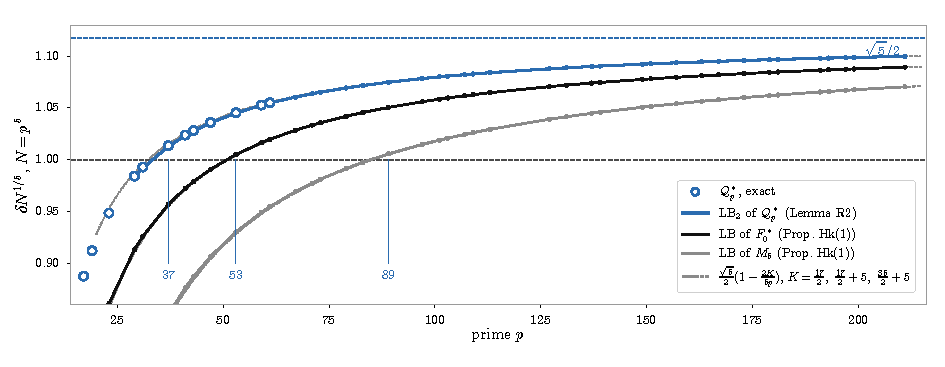
\includegraphics[width=\linewidth,height=0.45\textheight,keepaspectratio]{figs/col_half5.pdf}}{\fbox{\parbox{0.9\textwidth}{\centering figure \texttt{col\_half5} pending}}}
\caption{\colHalfCaption\interactive{beyond.html}}
\label{fig:half5}
\end{figure}

\emph{Searched designs.} Smaller constants than $B_s$ come from searched split-frame designs: random integer points with $u$ even and $v$ odd, then, column by column and level by level, short reachable columns (Proposition~\ref{prop:Gsplit}) in the coset $\frac12\mathbf h+\Z^{s-1}$ for a vector $\mathbf h$ of odd integers, found by lattice reduction; the diagonal is then chosen by evaluating the exact relaxation $\mathrm{LB}$ of Proposition~\ref{prop:Hk}(1), and it need not be dominant. The bound of Proposition~\ref{prop:HL5} is the exact value of the relaxation of Proposition~\ref{prop:Hk}(1); its design $H_5^*$ is also the one drawn in Figures~\ref{fig:arclarge}(c) and~\ref{fig:arcsplit}.

\begin{proposition}[Dimension five; computer-assisted]\label{prop:HL5}
Let $\mathcal H^{5*}_{k,p}=\mathcal P^{u,v,F}_{k,p}$ for the split frame $u=(-2,0,2,4,8)$, $v=(5,7,-1,3,1)$ and the design $F=H_5^*$ of Appendix~\ref{app:designs}. For every prime $p\notin\{2,3,5,7,97,101\}$ and every $k\ge1$ it is a digital $(0,5k,5)$-net over $\F_p$ with one point in every cell ($p=97,101$ enter only for $k\ge4$), and for every prime $p\ge1511$ and every $k\ge1$,
\[
\delta N^{1/5}>1.0265 .
\]
\end{proposition}

\begin{proof}[Proof (computer-assisted)]
The design $H_5^*$ satisfies (Half); its geometric layer $F_0$ has the row scalars $\lambda'=\frac12(-9,-3,-3,3,9)$ and the column scalars $\mu=(5,5,5,-5,1)$. The primes of the point differences, of the units $\lambda'_c\mu_d$ and of the leading coefficients of the column polynomials $g_{d,j}$ (exact interpolation) are $2,3,5,7$ and $97,101$, the last two only in leading coefficients at carry depth $j=3$; Proposition~\ref{prop:Gsplit} gives the net statement. For the separation, $\max|\sigma_c|=253$, so Proposition~\ref{prop:Hk}(1) applies for $p>506$; the monotone bound $\mathrm{LB}^*$, minimized over the number of design levels $L=\min(k,4)\in\{1,2,3,4\}$ (that is, over $k$), is $1.026529\ldots$ at $p=1511$, the same value as $\mathrm{LB}$ (attained at $L=4$, i.e. $k\ge4$). As $\mathrm{LB}^*$ is nondecreasing in $p$ for each $L$, $\delta N^{1/5}\ge\mathrm{LB}^*(p)\ge\mathrm{LB}^*(1511)=1.026529\ldots>1.0265$ for every prime $p\ge1511$ and every $k$.
\end{proof}

\emph{Dimension three.} $D_3^+$ has minimum $\sqrt3/2<1$, so the mechanism above gives nothing at $s=3$; whether other layers with entries of order $p$ and a rational limit $A=\lim\tilde M/p$ can be realized for every $k$ in dimension three is open (Remark~\ref{rem:open}(7)).

\section{Verification status}\label{sec:formal}
Every result is proved in the text, by hand or, where stated, with a computer-assisted finite certificate. The numbers in the paper fall into three classes.
\begin{itemize}
\item \emph{Computer-assisted proofs} rest on exact finite certificates: Propositions~\ref{prop:korobov4}, \ref{prop:4D2}, \ref{prop:HL5} and~\ref{prop:half5}; part (4) of Proposition~\ref{prop:wnet} (exact minimum distances at the primes $17\le p\le89$); the part of Theorem~\ref{thm:D} for layers that are not skew; the rows $s\le6$ of Table~\ref{tab:Kdesigns} and $s\ge4$ of Table~\ref{tab:practical} (with Proposition~\ref{prop:k1designs}); the values of Table~\ref{tab:S1E}; the per-prime certificates of Remark~\ref{rem:perprime} (Appendix~\ref{app:perprime}); and Theorem~\ref{thm:base23} (Table~\ref{tab:base23}). The certificates of Propositions~\ref{prop:korobov4}, \ref{prop:4D2}, \ref{prop:HL5} and~\ref{prop:half5}, of part (4) of Proposition~\ref{prop:wnet}, of Theorem~\ref{thm:D}, of Table~\ref{tab:S1E}, of Appendix~\ref{app:perprime}, of parts (2) and (3) of Theorem~\ref{thm:base23} and the per-prime completions of Proposition~\ref{prop:k1designs} are also checked in the Lean kernel. Part (1) of Theorem~\ref{thm:base23}, the entries $.4699$ and $.2586$ of Table~\ref{tab:base23}, and the thresholds and scans of Tables~\ref{tab:Kdesigns} and~\ref{tab:practical} are checked by scripts only (Appendix~\ref{app:formal}). The certificates of Theorems~\ref{thm:base23} and~\ref{thm:D}, Propositions~\ref{prop:4D2}, \ref{prop:half5}, \ref{prop:wnet} and~\ref{prop:k1designs} and Tables~\ref{tab:Kdesigns} and~\ref{tab:practical} were moreover reproduced by two independent implementations, that is, by two separately written programs (for Theorem~\ref{thm:base23}, two C++ checkers written from the mathematics, without shared code). The scripts of the accompanying software deposit (Appendix~\ref{app:verify}) rerun the certificates of Theorem~\ref{thm:base23}, Propositions~\ref{prop:half5} and~\ref{prop:wnet} and Theorem~\ref{thm:D}.
\item \emph{Computed values} are labelled where they occur and are used in no proof: the decay of the net of \cite{GK09} (Section~\ref{sec:intro}); the bracket of Remark~\ref{rem:cubecost}; the exact minimum distances of Table~\ref{tab:c}; the values $a^*_s$ of Table~\ref{tab:astar}; the rows $s=7,8$ of Table~\ref{tab:Kdesigns}; the effect of Remark~\ref{rem:projlines}; the per-prime nets listed after Corollary~\ref{cor:frameid} other than the one of Proposition~\ref{prop:korobov4}; the computed values after Proposition~\ref{prop:twocoset}, including the comparison with the column nets; those after Proposition~\ref{prop:wnet}, including the layer at $m=3$ in which two coordinates share their geometric digit (value $\sqrt{233}/15$ in the limit model of Section~\ref{sec:wnet}); the shifts of Remark~\ref{rem:wshift} that break the lock; the comparison of $\mathcal W^*_p$ with $\mathcal W_p$ in Remark~\ref{rem:wstar}; the comparison nets of Figure~\ref{fig:drift}(c), whose second digit is the same in all coordinates (Section~\ref{sec:drift}); the exact minimum distances of $\mathcal Q^*_p$ after Proposition~\ref{prop:half5}; the orbits after Theorem~\ref{thm:D}; and the values for $M_5$ in Remark~\ref{rem:M5}. Appendix~\ref{app:verify} lists the scripts that reproduce them.
\item \emph{Heuristic statements} are marked as such where they occur (for instance in Remarks~\ref{rem:glue}, \ref{rem:diag0}, \ref{rem:skelr0}, \ref{rem:skelconst} and~\ref{rem:S1Elim}, and the limit model of Section~\ref{sec:wnet}).
\end{itemize}

\emph{Lean.} Every theorem, proposition, lemma and corollary, every definition except Definition~\ref{def:geom} (which only introduces names), and the proved statements of the remarks listed in Table~\ref{tab:lean} are formalized in Lean~4 \cite{dMU21} with Mathlib \cite{Mathlib20}, apart from finite computations that are checked by scripts instead: part (1) of Theorem~\ref{thm:base23}, the tables of designs and the computed values above (the list is in Appendix~\ref{app:formal}). One formalized result, Proposition~\ref{prop:cube}, uses classical theorems that are not in Mathlib as explicit hypotheses: Haj\'os's theorem, Keller's conjecture for $s\le7$ and the optimal packing bounds in dimensions two and three; so does the growth statement for the design $U_s$ of Remark~\ref{rem:Us} (the prime number theorem). Consequences of other cited theorems, such as the asymptotics after Proposition~\ref{prop:E} and Theorem~\ref{thm:Lstar}, are cited and not formalized. Appendix~\ref{app:formal} describes the method and maps the sections of the paper to the statement files and proof modules of the formalization (Table~\ref{tab:lean}). The formal proofs complement, and do not replace, the arguments in the text.

\section{Open problems}\label{sec:remarks}
\fussy
We list what remains open, by the regimes of the lattice picture (Section~\ref{sec:prelim}): (I) geometric layers $\tilde M$ with entries bounded independently of $q$, at $m=sk$; (II) lattice skeletons, $m\not\equiv0\pmod s$; (III) layers with entries of size $\Theta(q)$. Results stated earlier are not repeated. Recall that the (first-order) deficit of a family of nets is the $K$ in $\delta N^{1/s}=1-K/q+O(q^{-2})$, and the certified deficit $K(F)$ of a design is the value that the one-digit relaxation certifies (Definition~\ref{def:K}).

\begin{remark}[Open problems]\label{rem:open}
\emph{(I) Bounded layers.} (1) \emph{Growth of the deficit.} Let $K(s)$ be the best first-order deficit $K$ in $\delta N^{1/s}=1-K/q+O(q^{-2})$, $q\to\infty$, over families of digital $(0,sk,s)$-nets over $\Z/q\Z$ whose geometric layers have entries bounded independently of $q$ and no zero diagonal entry. Lower bounds: $K(s)\ge\sqrt{(s-3)/8}$ (Theorem~\ref{thm:L}). For designs on the places $\infty,0,\dots,s-2$: $K(F)\ge s^{1-o(1)}$ (Theorem~\ref{thm:Lstar}); if moreover the row scalars $\lambda'_c$ (Proposition~\ref{prop:F}) take one value on the finite places, $K(F)\ge\operatorname{lcm}(1,\dots,s-3)$ (Proposition~\ref{prop:E}); and the two-axis bound $K_{\mathrm{pair}}$ is at least $2$ for $s\ge5$ (Theorem~\ref{thm:O5}). Upper bounds: the constructions here achieve $1$ for $s=3$, $2$ for $s=4$ (Proposition~\ref{prop:4D2}), $5$ and $10$ for $s=5,6$ (Table~\ref{tab:Kdesigns}), and a certified deficit at most $a^*_s\le e^{s\log s+O(s)}$ for every $s\ge4$ (Theorem~\ref{thm:A}). Does $K(s)$ grow polynomially or exponentially? On these places a certified deficit polynomial in $s$ would need row scalars that differ between the finite places (Proposition~\ref{prop:E}). Also open: $K=1$ for $s=4$; whether layers with zero diagonal do better (Remark~\ref{rem:diag0}); and the optimal second-order constant $C$ in $\delta N^{1/3}=1-1/p+C/p^2+o(p^{-2})$ in dimension three. For nets with the layer of $\mathcal P_{k,p}$ it is at most $4$ for $k\ge4$ (after Corollary~\ref{cor:ceil3}); for other bounded layers Proposition~\ref{prop:ceil}(i) bounds it by $\frac12\bigl((|\tilde M_{ba}|+1)^2+(|\tilde M_{b'a}|+1)^2\bigr)$ for a coordinate $a$ with $\tilde M_{aa}=-1$, and for zero diagonals (Remark~\ref{rem:diag0}) we have no bound. (2) \emph{Small bases.} Theorem~\ref{thm:A} needs $q\ge5a^*_s+4$, and the designs of Table~\ref{tab:Kdesigns} certify smaller bases only by finite scans; for $s=4$ the bases $q\le15$ have only weaker proved constants, and for $s\ge4$ Theorem~\ref{thm:A} excludes even $q$ (it needs $\operatorname{lpf}(q)\ge s-1$; for $q=2$ no $(0,m,s)$-net with $s\ge4$ exists, as $s\le q+1$). In dimension three the bases $2$ and $3$ are covered for every $m$ (Theorem~\ref{thm:base23}, computer-assisted); at $m=3$ the column nets cover every base coprime to $6$ (Theorem~\ref{thm:col}), column nets do not exist in even bases (Theorem~\ref{thm:O}), and the other bases $q\ge4$ divisible by $2$ or $3$ are open at $m=3$.

\emph{(II) Lattice skeletons.} (3) For $s\ge5$ the residues $1\le r\le s-3$ ($\ell\ge3$ skeleton coordinates) are open for all $p$; per-prime nets exist for $s=5$, $r=2$ at seven primes (computed, after Corollary~\ref{cor:frameid}), and a family for all large $p$ is open. Lattices with the optimal minimum order $p^{\ell/s}$ exist by a counting argument (after Lemma~\ref{lem:skellat}); explicit ones are known here only for $\ell=1$, $\ell=2$ and $r=1$, and for $3\le\ell\le s-2$ an explicit family is open (a mixed radix in the ring of integers of a degree-$\ell$ field is a natural candidate). The bottleneck is to realize such a skeleton with bounded faults: inside the frame orbit Lemma~\ref{lem:frameid} excludes the Korobov skeleton digits of $\mathcal B^1$ with small faults (Corollary~\ref{cor:frameid}); other Korobov vectors, faults growing slowly with $p$, and completions outside the frame orbit are not excluded, and per prime frame-orbit skeletons with faults $\pm1$ work (Proposition~\ref{prop:korobov4}). For one skeleton coordinate it is open whether the certified Euclidean constants tend to $\sqrt{\gamma_s}$ (Remark~\ref{rem:S1Elim}) and which explicit $\kappa$ attain it; for two skeleton coordinates, Euclidean (rather than maximum-norm) bounds are open. (4) In dimension four: $m\equiv1\pmod4$ for primes $p>83$ (no closed form is known; per-prime nets are known at every prime $7\le p\le83$, after Corollary~\ref{cor:frameid} (computed), Proposition~\ref{prop:korobov4} works out $p=13$, and we know of no obstruction for larger $p$), $m=4$, and small primes ($m\equiv1$ at $p=5$, $m\equiv2$ at $p\le19$, $m\equiv3$ at $p\le13$). Also open: an explicit $p_0(s)$ in Theorem~\ref{thm:S2} for $s\ge9$, and a covering radius uniform in $p$ for $\ell\ge2$. (5) In dimension three: a mesh ratio uniform in $p$ for $m\equiv1$; $m\in\{4,7\}$ for $p\le31$ and $m=5$ for $p\le7$; and an explicit family for all large primes with limit $>1$ at the resolutions $m\ge4$ (at $m=3$ the nets $\mathcal T_p$ and $\mathcal W_p$ of Propositions~\ref{prop:twocoset} and~\ref{prop:wnet} are such families). At $m=3$, among constants below $1$: whether digital $(0,3,3)$-nets that are not column point sets have smaller deficits than $\frac13$ and $\frac23$ (Theorem~\ref{thm:O} settles this among column point sets; outside them the drift-and-jitter bookkeeping of Section~\ref{sec:drift} is only a heuristic).

\emph{(III) Large-entry layers.} (6) (a) Smaller bases for $s\ge5$: Proposition~\ref{prop:HL5} needs $p\ge1511$, and at one resolution it is open whether some $(0,5,5)$-net over $\F_p$ with $p\le31$ has $\delta N^{1/5}>1$ (Proposition~\ref{prop:half5}). (b) The drift-and-jitter bookkeeping for half-integer layers at $k\ge2$, where the split-frame layers are Cauchy matrices, and for $s\ge6$. (c) Split-frame designs with explicit constants of moderate size for $s=6,7,8$. (d) Half-integer layers at the resolutions $m\not\equiv0\pmod s$. (e) Other split-frame layers beyond $D_s^+$. (7) In dimension three: whether a geometric layer $\tilde M\approx qA$ with a fixed rational matrix $A$ can be realized for every $k$ with $\delta N^{1/3}$ bounded above $1$. At $k=1$, layers whose geometric digits wrap together in two or three coordinates (locked wraps, Section~\ref{sec:wnet}) give the limits $\sqrt{66}/8$ (Proposition~\ref{prop:twocoset}), $\sqrt{281}/16$ (Proposition~\ref{prop:wnet}) and $\mu^*=1.0480\ldots$ (Remark~\ref{rem:wstar}), the optimum of the layers of rank one with image $\F_p(2,2,1)$ (Proposition~\ref{prop:wfamily}); the optimum over the other images of rank one, over layers of rank two and over non-digital point sets is open. At $k\ge2$ the geometric digits of any two coordinates are jointly uniformly distributed (Lemma~\ref{lem:shared}, as $2(k+1)\le3k$), so no relation between the geometric digits of two coordinates survives, and neither the two-coordinate lock of $\mathcal T_p$ nor the three-coordinate lock of $\mathcal W_p$ extends to $k\ge2$. For digital nets the only linear relation among the three geometric digits of one index that this count leaves is one of full support, $h_xr_x+h_yr_y+h_zr_z\equiv0$ with all $h_c\ne0$; whether such a relation, or a correlation that involves digits of other indices, can raise the constant above $1$ is open.

\emph{The case $k=1$ and digital shifts.} (8) At $k=1$: whether $K_1=1$ is possible for $s=5$, or $K_1=2$ for $s=6$ (Proposition~\ref{prop:k1designs}); frameless layers ($F_0$ chosen directly, not from a frame, Proposition~\ref{prop:k1designs}(2)) for $s\ge7$; and the choice of the deeper rows, which are free at $k=1$ apart from $t=0$ and change the exact separation at small $q$ (Proposition~\ref{prop:k1} and the remark after it). (9) In the bases two and three the constants of Theorem~\ref{thm:base23}(3) are certified lower bounds, not exact values; for $b=3$ and $m\equiv2\pmod3$ the infimum over $m$ and $\tau$ for these nets lies between $0.0770$ and $0.0901$, the latter the exact value at $m=20$ (computed). Whether other seeds or lift parameters give larger every-shift constants in base three is open.

\emph{Sequences.} (10) All nets here depend on $m$; they are not prefixes of one sequence, and the question of \cite{DGS2} for sequences remains open in dimension $s\ge3$.

\emph{Beyond digital nets.} (11) Can nets that are not digital, for instance permutation nets, exceed the constants of the digital nets here, for instance by avoiding the slip planes that linear offsets force (Corollary~\ref{cor:linoff})?
\end{remark}

\section{Relation to prior work}\label{sec:prior}
Where we say below that we found no prior work, this reflects a literature search (web searches of October 2026) that was not exhaustive; it is not a claim of priority.
\emph{The frame and unit minors.} The unit-minor criterion over any finite commutative ring is Niederreiter's \cite[Thm.~6.1]{Nie87}; the M\"obius frame $(T^2,I,T)$ of Section~\ref{sec:frames}, which by Proposition~\ref{prop:faure} is the net with the generator matrices $(J,P,I)$ up to scrambles, is his construction \cite[Thm.~6.2]{Nie87} with the elements $\beta=(0,1)$ of $\F_q$, whose box determinants are $\pm\prod(\beta_k-\beta_h)^{d_hd_k}=\pm1$, and \cite[Cor.~6.3]{Nie87} gives $(0,m,3)$-nets in every base (Theorem~6.2 is stated over a product of finite fields; since the determinant identity is polynomial, the same integer matrices work over $\Z/q$ by Theorem~6.1). For integer systems the reduction to prime-power and prime moduli is \cite[Lemmas~8--9]{LNS96}, and the admissible dimensions over a ring, in particular $s\le\operatorname{lpf}(q)+1$ over $\Z/q\Z$, are \cite[Thm.~2, Cor.~2]{LNS96}; Lemmas~\ref{lem:hermite} and~\ref{lem:Ts} are therefore classical in substance. The same matrices reappear as universally decodable matrices in coding theory \cite{VG06}.
\emph{Scrambles and $t$-preserving moves.} That lower-triangular scrambles preserve $t$ is standard \cite{Mat98,Tez95,DP10} (as do Owen's nested scrambles \cite{Owe95}, a nonlinear family that contains the lower-triangular ones); Proposition~\ref{prop:faure} places $\mathcal P_{k,q}$ in Tezuka's generalized Faure class (for each $m$). Lemma~\ref{lem:box} (the gauge moves, which preserve $t$) is elementary; the block scalings are not per-coordinate lower-triangular scrambles (whether they leave the orbit of the nested scrambles we have not checked), and the nets $\mathcal B^1$ use them. The occupied fine cells of $\mathcal B^1$ form, per coarse block, cosets of a Korobov lattice \cite{Kor59,SJ94}.
\emph{Separation.} In two dimensions, well-separated nets are known: the Larcher--Pillichshammer net \cite{LP01,DGS2} and, in coding language, a digitally shifted Hammersley set with a product-distance bound \cite{TV06}. In every dimension Sobol' and Shukhman \cite{SS07} bound the minimum distance of Sobol' points from below, by a bound that decays faster than $N^{-1/s}$. Without the digital structure, quasi-uniform low-discrepancy point sets are known in every dimension: Frolov point sets \cite[Thm.~3.1]{DGLPS1}, Kronecker sequences \cite[Thm.~3.9 and the text after Cor.~3.13]{DGLPS1} (with discrepancy $N^{-1+\varepsilon}$), and (by an existence argument) rank-$1$ lattices \cite[Thm.~3.7]{DGLPS1}. These are not digital nets in a fixed base (Section~\ref{sec:intro}), and we do not claim the broad statement. In two dimensions the even-$m$ permutation nets of \cite[Sec.~3]{GK09} follow the pattern of this paper: a lattice of lines, van der Corput slides along these lines carrying $t=0$, and a torus tiling adapted to that lattice (Remark~\ref{rem:gk2d}; their net property is proved in \cite{Rud26}).
\emph{Large-entry layers.} The packings $D_s^+$ and $E_8$ are classical \cite{CS99}, and so are the bounds of Cohn and Elkies \cite{CE03} and the optimality of $E_8$ \cite{Via17}. We found no digital nets with a $D_s^+$ or $E_8$ local structure, and no construction that reads the cell and the offset of a coordinate at different points, as the split frames of Section~\ref{sec:large} do. Their box-minor lemma (Lemma~\ref{lem:Tsplit}) is classical in substance: it is the confluent Vandermonde determinant of Hermite interpolation, as in Niederreiter's frames \cite[Thm.~6.2]{Nie87}. Suzuki \cite{Suz26} studies the separation of scrambled digital nets: under full Owen scrambling fixed-$t$ nets are not quasi-uniform (the mesh ratio is $\Omega(N^{1/(2s)})$ in probability), and matrix (linear) scrambling of binary fixed-$t$ digital nets gives mesh ratio $O(\log N)$ in probability in every dimension $s\ge2$. Both results are in probability, for randomized nets, and short of quasi-uniformity; they do not overlap with the explicit constructions here. They concern random scrambles; a particular nested scramble can be well separated: the two-dimensional nets of Remark~\ref{rem:gk2d} are a nested scrambling \cite{Owe95} of the Hammersley net (Remark~\ref{rem:gk2d}(iv)), and they are not digital \cite{GK09,Rud26}. The closest work we found is: \cite{DGS2}, whose quasi-uniform digital example is two-dimensional; He \cite{He17,He21}, who builds rotated sphere packing designs and designs from rotated lattices (rotated $\Z^s$, densest packings including $E_8$, thinnest coverings, interleaved lattices) with quasi-optimal separation distance on all projections, which are not digital nets; He \cite{He19}, who builds maximin designs from interleaved lattices (unions of shifted copies of a lattice), which are not nets; and the search for $(t,m,s)$-nets with maximized minimum distance \cite{GHSK08,GK09}. $D_s$ is Construction~A of the even-weight code, and for even $s$, $2D_s^+$ is Construction~D applied to the repetition code contained in the even-weight code \cite{BS83}; whether such one-point-per-cube descriptions have been used for nets before we have not checked systematically.
\emph{One point per cube.} The theorems behind Proposition~\ref{prop:cube} are classical: Haj\'os's theorem on lattice cube tilings \cite{Haj42}, Keller's conjecture, proved for $s\le6$ by Perron \cite{Per40} and for $s=7$ by Brakensiek, Heule, Mackey and Narv\'aez \cite{BHMN20}, and false for $s\ge8$ \cite{LS92,Mac02}, and the optimality of the face-centred cubic packing \cite{Hal05}, of $E_8$ \cite{Via17} and of the Leech lattice \cite{CKMRV17}. We found no prior use of the cube-tiling theorems for the separation of nets. Maximin Latin hypercube designs, in which every coordinate takes each of $N$ grid values exactly once, have separation bounds under this marginal one-per-row constraint \cite{vDHHM07,vDRH09}; we found no prior separation analysis under the constraint of one point per cube.
\emph{Codes.} Each ingredient of Remark~\ref{rem:codes} is classical: Construction~A and Construction~D \cite{CS99,BS83}, the characterization of MDS codes by nonsingular submatrices \cite{MS77} and of generalized Reed--Solomon codes by Cauchy redundancy matrices \cite{RS85}, the spectral test \cite{CM67,Knu97}, and the equivalence of $t=0$ with the MDS property in the Rosenbloom--Tsfasman metric, with Reed--Solomon codes of that metric \cite{RT97,Skr01,Nie87}; over a field, the zero count after Lemma~\ref{lem:hermite} is Skriganov's MDS proof for these codes. We found no prior work that relates the Euclidean separation of digital nets to Construction~A, Lee-metric codes or the spectral test, and no treatment of digital-net skeletons as generalized Reed--Solomon Construction~A lattices or of geometric layers $\tilde M\approx qA$ with $A$ rational of denominator $e$ as codes over $\Z/e^2$. The carry criterion of Corollary~\ref{cor:linoff}(b) is the analogue, for carries, of the criterion of Kositwattanarerk and Oggier \cite{KO14}: the code formula $C_0+2C_1+\dots+2^{a-1}C_{a-1}+2^a\Z^n$ of nested binary linear codes is a lattice if and only if the codes are closed under the Schur product, whereas Construction~D always gives a lattice.
\emph{What is new.} We did not find the following in the literature.
\begin{itemize}
\item Part~I: the scramble $L$; the residue description of the geometric digits (Proposition~\ref{prop:cell} and Lemma~\ref{lem:Rs}); a single choice of scrambles that realizes a design for every number $k$ of cell digits (Proposition~\ref{prop:Gs}); a separation bound of the optimal order $N^{-1/s}$ for a family of digital nets in a fixed base ($N=q^m$, $m\to\infty$) in any dimension $s\ge3$ (decaying lower bounds are known \cite{SS07}); the lattice of admissible design columns with its adelic Chebyshev identity (Lemmas~\ref{lem:sat}, \ref{lem:adelic}); the deep-shift lift $m\to m+3$ (Definition~\ref{def:lift}), which carries a separation certificate (Lemma~\ref{lem:liftsep}); and lattice skeletons of digital nets for the resolutions $m\not\equiv0\pmod s$ (Section~\ref{sec:skel}; the lattices themselves are classical congruence and Korobov lattices).
\item Column nets: column nets themselves and an exact minimum-distance formula for point sets on lines parallel to the body diagonal (Theorems~\ref{thm:colmin} and~\ref{thm:col}); their two-dimensional analogue is the union of translated diagonals with van der Corput slides of \cite[Sec.~3]{GK09}, and exact formulas are known for particular two-dimensional nets: the $\ell^\infty$ separation of the Sobol' points \cite{Suz25} and the dispersion of the Hammersley net \cite{Kri21}. Also the optimality of the column nets among column point sets and the column ceiling (Theorem~\ref{thm:O}(3), Corollary~\ref{cor:colceil}; part (2) of Theorem~\ref{thm:O} is classical in substance \cite{Pai51,HP55}).
\item Part~II: ceilings of the type of Proposition~\ref{prop:ceil} and Theorem~\ref{thm:L}; lower bounds for the certified deficit of frame designs by counting cross-ratios (Theorem~\ref{thm:Lstar}); the bookkeeping of the first-order deficit by drift and jitter with its holonomy obstruction (Lemma~\ref{lem:drift}); the description of the local configurations of digital nets by linear offsets, with the one-point-per-cube ceilings of Section~\ref{sec:whylat}; split frames with their non-symmetric Cauchy layers, and digital nets whose separation exceeds the cubic value $1$ at every resolution $m=sk$ (Theorem~\ref{thm:HL}); digital $(0,5,5)$-nets with $\delta N^{1/5}>1$, and the least drift $\mathrm{dr}=\frac{17}2$ over the half-integer layers of Theorem~\ref{thm:D} (Proposition~\ref{prop:half5}); explicit digital $(0,3,3)$-nets whose local configuration is a union of two lattice cosets, with separation above the cubic value (Proposition~\ref{prop:twocoset}); and a digital $(0,3,3)$-net with a layer of rank one and $\delta N^{1/3}\to\sqrt{281}/16$, with the optimum $\mu^*$ of its family (Propositions~\ref{prop:wnet} and~\ref{prop:wfamily}).
\end{itemize}
More generally, we found no digital $(0,3,3)$-net (polynomial lattice point sets included, as they are digital nets) with separation above the cubic value in the literature; the closest constructions we found are lattices, not nets: lattice designs \cite{He17,He21}, some of them built from packings denser than the cubic lattice, and the quasi-uniform rank-$1$ and Korobov lattice designs of Sakai and Goda \cite{SG26}.

\subsection*{Use of AI systems}
The constructions, proofs and Lean formalization were produced by AI systems (Anthropic Claude Opus~5.5; some early exploratory results used Claude Fable~5.1) under the author's direction. The author selected the problems, steered the research and reviewed the formal statements, but has not verified every proof by hand. AI systems are not listed as authors; responsibility for the deposit rests with the author.

\appendix

\section{Designs}\label{app:designs}
A design $(F_0,\dots,F_{L-1})$ prescribes, for each pair of coordinates $(c,d)$, how the geometric digit of $c$ depends on the last $L$ cell digits of $d$ (Section~\ref{sec:prelim}). With Definition~\ref{def:Ns} each design below defines the nets $\mathcal P^F_{k,q}$; the deficits and base thresholds they certify are in Table~\ref{tab:Kdesigns}, and the values at $k=1$ in Table~\ref{tab:practical}. Conventions: entry $(c,d)$ is in row $c$ and column $d$, with the coordinates in the order of the places listed; $F_n$ is the target at carry depth $n$ (the level $k-1-n$) of row $0$ of the block $(c,d)$, diagonal included.

\subsection{The designs of Table~\texorpdfstring{\ref{tab:Kdesigns}}{tab:Kdesigns}}
\emph{$s=4$}, places $(\infty,0,1,2)$, row scalars $\lambda'\equiv1$; this is the deficit-two design of Proposition~\ref{prop:4D2}:
\[
F_0=\begin{psmallmatrix}-2&-2&-1&-2\\1&-2&1&1\\1&-2&-2&2\\1&-1&-1&-1\end{psmallmatrix},\ F_1=\begin{psmallmatrix}0&3&1&1\\0&1&-2&-1\\-1&1&0&-3\\-2&1&0&0\end{psmallmatrix},\ F_2=\begin{psmallmatrix}0&-2&-1&0\\0&0&1&-1\\0&0&0&0\\1&0&1&0\end{psmallmatrix}.
\]
\emph{$s=5$}, places $(\infty,0,1,2,3)$, row scalars $\lambda'=(\frac12,1,1,1,1)$ (Proposition~\ref{prop:F}; the $\frac12$ needs $q$ odd):
\[
F_0=\begin{psmallmatrix}-4&-3&1&-1&3\\-1&-5&-2&1&-2\\-1&-6&-5&2&-3\\-1&-3&2&-5&-6\\-1&-2&1&-2&-5\end{psmallmatrix},\ F_1=\begin{psmallmatrix}-1&5&-1&1&-8\\1&0&-2&-2&4\\0&-2&0&-6&5\\-1&2&-6&1&4\\-2&2&-2&-2&1\end{psmallmatrix},\]
\[
F_2=\begin{psmallmatrix}1&0&1&1&4\\-1&1&1&0&-3\\1&5&1&3&-4\\2&2&1&0&1\\2&1&1&3&1\end{psmallmatrix},\ F_3=\begin{psmallmatrix}0&-2&-1&-1&1\\1&0&1&1&0\\-1&3&0&1&1\\-1&-3&3&0&0\\0&-1&0&-1&-1\end{psmallmatrix}.
\]
\emph{$s=6$}, places $(\infty,0,1,2,3,4)$, $\lambda'=(\frac12,1,1,1,1,1)$:
\[
F_0=\begin{psmallmatrix}-8&-6&3&1&-3&6\\2&-9&-6&-1&2&-3\\2&-12&-8&-2&3&-4\\2&-6&6&-7&6&-6\\2&-4&3&2&-9&-12\\2&-3&2&1&-6&-9\end{psmallmatrix},\ F_1=\begin{psmallmatrix}-1&7&-7&-1&7&-13\\-1&-1&2&0&-6&5\\-2&-10&0&-2&-10&6\\-3&1&-26&-1&-26&7\\-4&2&-10&-6&2&2\\-5&2&-6&-2&2&1\end{psmallmatrix},\ F_2=\begin{psmallmatrix}0&-4&0&1&-9&10\\1&4&2&0&7&-1\\0&20&1&4&11&0\\0&9&26&-1&23&3\\1&4&5&0&-2&8\\3&2&2&1&-1&1\end{psmallmatrix},\]
\[
F_3=\begin{psmallmatrix}1&8&7&-1&2&-4\\-2&-3&-1&0&-4&0\\1&3&0&-1&-7&0\\1&-3&-6&3&-3&1\\0&-1&-1&3&3&0\\0&0&1&-1&2&0\end{psmallmatrix},\ F_4=\begin{psmallmatrix}-1&-3&-3&-3&3&1\\0&4&0&1&1&-1\\-1&-1&1&1&3&-2\\0&-1&0&-2&0&-5\\3&-1&3&1&-1&1\\0&-1&1&1&0&3\end{psmallmatrix}.
\]
Each design is reachable: the interpolating polynomials $g_{d,j}$ of Proposition~\ref{prop:F} have degree $j$ and leading coefficients that are units of the ring $R'$ of Definition~\ref{def:Ns} (checked by exact interpolation). The designs for $s=7,8$ are in the software deposit (Appendix~\ref{app:verify}).

\subsection{The layers of Table~\texorpdfstring{\ref{tab:practical}}{tab:practical}}
At $k=1$ a design is a single geometric layer $F_0$, of two kinds (Proposition~\ref{prop:k1designs}). The \emph{frame layers} are, off the diagonal, the Cauchy layers $\lambda'_c\mu_dw_{cd}$ that every scrambled frame on the places $\infty,0,1,\dots,s-2$ has (Proposition~\ref{prop:Ns}), with a diagonal chosen for $k=1$: for $s=4$ the off-diagonal part of $U^*_4$, for $s=5$ that of the $s=5$ design of Table~\ref{tab:Kdesigns}, and for $s=6$ the searched scalars $\lambda'=(1,\frac23,-2,-\frac23,\frac23,-2)$, $\mu=(\frac32,18,3,3,9,6)$:
\[
\begin{psmallmatrix}-1&2&1&2\\1&-1&-1&-1\\1&2&-2&-2\\1&1&1&-2\end{psmallmatrix},\qquad \begin{psmallmatrix}-3&-3&1&-1&3\\-1&-3&-2&1&-2\\-1&-6&-3&2&-3\\-1&-3&2&-3&-6\\-1&-2&1&-2&-3\end{psmallmatrix},\qquad \begin{psmallmatrix}-6&18&3&3&9&6\\1&-4&-2&-1&-2&-1\\-3&-36&-6&6&9&4\\-1&-6&-2&-6&6&2\\1&4&1&2&-4&-4\\-3&-9&-2&-3&-18&-3\end{psmallmatrix}.
\]
The \emph{frameless layers}, integer matrices chosen directly, for which a $t=0$ completion exists for each admissible prime ($s=5$, $K_1=2$; $s=6$, $K_1=3$; $s=6$, $K_1=5$), are
\[
\begin{psmallmatrix}-2&1&-1&-2&-1\\-1&-2&-2&2&-1\\-1&1&-1&-1&2\\-2&1&-2&-2&1\\-1&-2&1&1&-2\end{psmallmatrix},\qquad \begin{psmallmatrix}-3&-3&2&-1&2&1\\1&-3&2&1&3&-2\\1&-2&-3&3&-1&-1\\2&3&1&-2&-1&1\\-3&-2&1&1&-3&2\\-1&-1&3&2&2&-3\end{psmallmatrix},\qquad \begin{psmallmatrix}-4&1&3&-1&2&4\\-2&-4&1&-1&1&3\\-4&-2&-4&4&1&-2\\-2&4&-2&-4&-4&-2\\1&-3&3&1&-5&2\\-1&4&4&-2&1&-5\end{psmallmatrix};
\]
their deeper rows are chosen per prime factor of $q$ (Proposition~\ref{prop:k1designs}). For the finitely many admissible primes below the Schwartz--Zippel bound $\mathrm{SZ}(s)$ of that proof, where the generic argument does not apply, explicit completions with $t=0$ were constructed and checked; they are in the deposit.

\subsection{The five-dimensional split-frame design \texorpdfstring{$H_5^*$}{H5*}}
This design gives the nets $\mathcal H^{5*}_{k,p}$ of Proposition~\ref{prop:HL5}, with $\delta N^{1/5}>1.0265$ for every prime $p\ge1511$. Its split frame (Definition~\ref{def:split}) has the offset points $u=(-2,0,2,4,8)$ and the cell points $v=(5,7,-1,3,1)$; the conventions are those stated at the start of this appendix:
\[
2F_0=\begin{psmallmatrix}-147&5&45&-9&3\\3&-61&-15&-5&3\\5&3&-53&-15&-3\\-15&-5&3&-61&1\\15&45&5&-9&-45\end{psmallmatrix},\quad
F_1=\begin{psmallmatrix}0&23&21&12&-1\\-2&0&38&5&-2\\-3&15&0&-10&-1\\4&-28&-4&0&0\\-14&-18&-6&21&0\end{psmallmatrix},
\]
\[
F_2=\begin{psmallmatrix}0&-19&-54&-7&-2\\-1&0&-39&-2&1\\-2&-13&0&19&2\\2&26&0&0&-1\\5&-6&-1&-18&0\end{psmallmatrix},\quad
F_3=\begin{psmallmatrix}0&-7&10&-1&1\\1&0&8&-1&-1\\2&-4&0&-2&0\\1&4&2&0&0\\1&1&4&1&0\end{psmallmatrix}.
\]
Off the diagonal, the geometric layer is $M^{(0)}_{cd}=\lambda'_c\mu_d/(u_c-v_d)$ with $\lambda'=\frac12(-9,-3,-3,3,9)$ and $\mu=(5,5,5,-5,1)$; all partial sums $M^{(j)}$ lie in $\frac12+\Z$ (off-diagonal entries of absolute value at most $\frac{87}2$), and $M^{(3)}=-\frac12$ off the diagonal. The interpolating polynomials $g_{d,j}$ of Proposition~\ref{prop:Gsplit} have degree $j$, and their leading coefficients have only the primes $2,3,5,7$, except $-97$ ($d=1$, $j=3$) and $\frac{101}{12}$ ($d=2$, $j=3$). This is why Proposition~\ref{prop:HL5} excludes $p\in\{2,3,5,7,97,101\}$, and why $97$ and $101$ matter only from $k\ge4$ on, when carry depth $3$ is used.

\section{Deferred proofs and side results}\label{app:proofs}
This appendix holds one deferred proof and two heuristic remarks.
\subsection{Proof of Proposition~\ref{prop:P2}}
\begin{proof}
Let $e=\e_a+\varepsilon\e_b$ be the step of the proposition, from the cell $n$ to the cell $n+e$. Write $\rho'_b$ and $\rho''_b$ for the second offset digit of $b$ at $n$ and at $n+e$; along $e$ it changes by a constant $\sigma'_b$ modulo $q$. Count the cells $n$ with the following properties:
\begin{enumerate}
\item[(a)] the last digits of $n_a$ and $n_b$ cause no carry along $e$;
\item[(b)] $r_a+\sigma_a\ge q$, so that $a$ wraps ($\sigma_a$ values of $r_a$);
\item[(c)] $r_b$ does not wrap ($q-|\sigma_b|$ values);
\item[(d)] $\rho'_b$ lies in a nonempty set $\mathcal V_b$ of digit values chosen so that $\varepsilon(\rho''_b-\rho'_b)\le0$;
\item[(e)] $r_u+\sigma_u\in[0,q)$ for every coordinate $u\notin\{a,b\}$.
\end{enumerate}
For one $u$ at a time, the digits involved form a box with depths $k+1$ on $a$, $k+2$ on $b$, $k+1$ on $u$ and $0$ elsewhere, of total $3k+4\le sk$, so they are jointly uniform; the conditions (a)--(d) have positive density and the fraction of cells violating (e) at $u$ is $|\sigma_u|/q$, so some cell satisfies all of them, because $\sum_u|\sigma_u|<q$. For such a cell, $|\Delta_a|<(\sigma_a+1)/q$, $|\Delta_u|<(|\sigma_u|+1)/q$ and $\varepsilon\Delta_b<1-|\sigma_b|/q+1/q^2$. The second part of the proposition (the case $\varepsilon\sigma_b>0$) uses, in the same way, the boxes with depths $k+1$ on $a$, $b$ and $u$ and $0$ elsewhere (total $3k+3\le sk$), with $r_a$ and $r_b$ both wrapping, so that $|\Delta_a|<(\sigma_a+1)/q$ and $|\Delta_b|<(|\sigma_b|+1)/q$. The pair lies inside the cube, so the bound holds for the toroidal and the Euclidean distance.
\end{proof}
\subsection{A conjectural limit for one skeleton coordinate (heuristic)}
\begin{remark}[The limit $\sqrt{\gamma_s}$]\label{rem:S1Elim}
Table~\ref{tab:S1E} suggests that $\max_\kappa\lambda_{\mathrm{jit}}(\kappa)p^{-1/s}\to\sqrt{\gamma_s}$, the square root of the Hermite constant ($1.122$, $1.189$, $1.231$, $1.290$, $1.345$, $\sqrt2$ for $s=3,\dots,8$); here $\lambda_{\mathrm{jit}}(\kappa)$ is the Euclidean minimum of the skeleton lattice $\Lambda_\kappa$ after one fine cell of jitter is subtracted in each coordinate (Proposition~\ref{prop:S1E}). The upper bound holds by the definition of $\gamma_s$, since $\lambda_{\mathrm{jit}}\le\lambda_2(\Lambda_\kappa)\le\sqrt{\gamma_s}\,p^{1/s}$. For the lower bound it would suffice that the index-$p$ sublattices of $\Z^s$, scaled to covolume $1$, equidistribute in $\mathrm{SL}_s(\Z)\backslash\mathrm{SL}_s(\R)$ as $p\to\infty$. Indeed, the set of unimodular lattices with $\lambda_1>\sqrt{\gamma_s}-\varepsilon$ is open and nonempty, so for large $p$ it would contain a scaled $\Lambda_\kappa$ ($\lambda_1$ is continuous, and the sublattices containing a unit vector have normalized minimum at most $p^{-1/s}$), and then $\lambda_{\mathrm{jit}}\ge\lambda_2-\sqrt s$. Such equidistribution is a theorem of Clozel, Oh and Ullmo on Hecke points \cite{COU01}, but as usually stated it is for simply connected $G$ and Hecke operators $T_a$ with $a\in G(\mathbb Q)$, which does not literally contain the index-$p$ correspondence of $\mathrm{diag}(p,1,\dots,1)\notin\mathrm{SL}_s(\mathbb Q)$. The version of Eskin and Oh \cite[Thm.~1.2]{EO06} allows $a$ in the commensurator of the arithmetic group; we have not carried out the reduction in detail, so we do not state the limit as a theorem. The limit would hold at the residue $m\equiv-1\pmod s$, as $p\to\infty$ uniformly in $k$, and would exceed the limit $\min(\sqrt s/2,\sqrt2)$ of Theorem~\ref{thm:HL} (at the residue $m\equiv0$) for $4\le s\le7$ and equal it at $s=8$.
\end{remark}

\subsection{Size of the constants in Theorem~\ref{thm:S2} (heuristic)}
\begin{remark}[Constants]\label{rem:skelconst}
$B(p)$ and $\rho(p)$ are nondecreasing, so the bounds are positive for every $p\ge p_0$. For $s\ge5$ a rough count gives $B\approx(p/\sqrt2)^{2/s}$, i.e. $\delta N^{1/s}\to2^{-1/s}$ (heuristic). For $s\ge9$ the route of Lemma~\ref{lem:G2N1}(c) needs $B$ of order $(2s/\pi)^2$, which suggests $p_0(s)=e^{O(s\log s)}$ (heuristic). Nothing is optimized: the faults cost $g^*$ cells at small $p$, and for even $r$ a \emph{block radix}, in which each of the two rows of $A$ is a radix chain on its own group of the full coordinates, has a better constant.
\end{remark}

\section{Per-prime designs in dimension three}\label{app:perprime}
\begingroup\small
With Theorem~\ref{thm:base23} ($p=2,3$) and Corollary~\ref{cor:allm} ($p\ge37$), these designs give well-separated families of digital $(0,m,3)$-nets in every prime base (Remark~\ref{rem:dgsfinite}). Proposition~\ref{prop:ppsep} reduces the separation bound of Table~\ref{tab:perprime}, for every $k$ and every graph form with the prescribed rows, to one finite computation per design; Propositions~\ref{prop:pp2} and~\ref{prop:pp1} show by hand that a net with the prescribed rows exists for every $k$ if the design satisfies finitely many polynomial conditions modulo $p$, which hold for the $37$ designs. All of this is formally verified (Proposition~\ref{prop:pp1} for odd $p$; every tabulated design has $p\ge5$). The appendix sets up the notation, defines the invariants of the moves, proves existence for every $k$, proves the separation bound for every $k$, and lists the finite checks.

\emph{Setting.} We use the notation of Section~\ref{sec:allm}: $p$ is prime, $m=3k+r$, $r\in\{1,2\}$, the depths are $\mathbf k=(k+1,k,k)$ resp. $(k+1,k+1,k)$, and $\Phi^F$ is the integer graph form of the frame with depths $\mathbf k$; all its box minors are $\pm1$. An offset row is named by its coordinate and its position: $X0$ is the first offset row of $x$, $Y1$ the second offset row of $y$, and so on. The \emph{prescribed rows} are the first offset row of a full coordinate and the first two offset rows of a skeleton coordinate: $X0,Y0,Z0=S_z,Z1$ for $r=2$, and $X0,Y0=S_y,Y1,Z0=S_z,Z1$ for $r=1$. The first offset row of a skeleton coordinate is its skeleton digit (Section~\ref{sec:skel}). The other prescribed row of each coordinate gives its \emph{inner digit}: the first digit after the fine cell of the point (Section~\ref{sec:fine}), which places the point inside its fine cell up to $1/p$ of the fine unit. For a full coordinate the inner digit is the first offset digit, the analogue of the geometric digit (Definition~\ref{def:geom}); Lemma~\ref{lem:skelred} counts it among the deeper digits, whereas the designs below prescribe it. $R|d_l$ is the coefficient of an offset row $R$ on level $l$ of the cell of $d$, and for rows $R,R'$ and columns $c,c'$ (levels, possibly of different coordinates) $[R,R'\,|\allowbreak\,c,c']=R|c\;R'|c'-R|c'\;R'|c$. The \emph{window} of the cell of $d$ is its last $L_d$ levels, $L_x=4$ if $r=1$ and $L_d=3$ otherwise.

\begin{definition}\label{def:ppdesign}
A \emph{per-prime design} for $(p,r)$ assigns to each prescribed row $R$ and each coordinate $d$ integers $R|d^{(i)}$, $0\le i<L_d$. A graph form over $\F_p$ with depths $\mathbf k$ \emph{carries} it if (i) each prescribed row $R$ has the coefficient $R|d^{(i)}\bmod p$ on level $k_d-1-i$ of $d$ and $0$ on the higher levels of $d$, and (ii) each offset row of $c$ below its prescribed rows has the coefficient $0$ on the cell of $c$.
\end{definition}

A per-prime design is the analogue, for the unequal depths $\mathbf k$, of a design with $L_d$ levels (Section~\ref{sec:prelim}): $R|d^{(i)}$ is the target at carry depth $i$ of $d$, diagonal included. In this appendix ``design'', ``configuration'', ``certificate'' and ``relaxation'' always mean the per-prime notions defined here. The upper index $i$ counts the levels from the last one and does not depend on $k$; in the proofs, which work at a fixed $k$, we write the entries with the level names of that $k$ instead (e.g. $Y0|x_{k-1}$ for $Y0|x^{(1)}$). Entries of a row of $c$ on the cell of $c$ are diagonal entries (Lemma~\ref{lem:box}); they matter for separation, not for existence. The $11$ designs that the coverage of every prime base needs ($m\equiv1$ for $5\le p\le31$, $m\equiv2$ for $p=5,7$; Remark~\ref{rem:dgsfinite}) are printed in Table~\ref{tab:ppdesigns}. The other $26$ designs of Table~\ref{tab:perprime} are at primes that other results already cover; they give larger constants there (Remark~\ref{rem:perprime}). All $37$ designs are fixed data of the formalization (Table~\ref{tab:lean}, statement file \texttt{Appendix}). For instance, for $p=5$, $r=2$ the skeleton digit is $S_z=2x_k-y_k$, so the occupied fine cells are those of the index-$5$ lattice $P_z\equiv2P_x-P_y\pmod5$, as for $\mathcal B^2$. The designs were found by a finite search scored by the relaxation of Definition~\ref{def:pprelax}; no optimality is claimed.

\smallskip\noindent\emph{Invariants of the frame.} The moves of Lemma~\ref{lem:box} scale and combine rows and levels. So a design can be carried by a graph form obtained from $\Phi^F$ by the moves only if every quantity that the moves do not change has the same value at the design as at $\Phi^F$. The following ratios are such quantities (Lemma~\ref{lem:ppinv}). Propositions~\ref{prop:pp2} and~\ref{prop:pp1} show that their values, together with finitely many conditions of vanishing and nonvanishing, suffice for existence at every $k$. For $r=2$ let $\tilde x=x_{k-1}-(Z0|x_{k-1}/Z0|x_k)\,x_k$ (a combination of columns), define $\tilde y$ likewise, and
\[
\chi_1=\frac{Z1|\tilde y\cdot Y0|\tilde x\cdot X0|y_k\cdot Z0|x_k}{Z1|\tilde x\cdot Y0|x_k\cdot X0|\tilde y\cdot Z0|y_k},\qquad
\chi_2=\Bigl(\frac{Z1|x_k}{Z0|x_k}-\frac{Z1|y_k}{Z0|y_k}\Bigr)\frac{Z0|x_k\cdot Y0|\tilde x}{Z1|\tilde x\cdot Y0|x_k}.
\]
For $r=1$ write $\xi_i=x_{k-i}$, $\eta_i=y_{k-1-i}$, $\zeta_i=z_{k-1-i}$; let $R_Y=Y1-(Y1|\xi_0/Y0|\xi_0)Y0$ and $R_Z=Z1-(Z1|\xi_0/Z0|\xi_0)Z0$ (combinations of rows), $d_x=[Y0,Z0\,|\allowbreak\,\xi_0,\xi_1]$, $\tilde\zeta=\zeta_1-(X0|\zeta_1/X0|\zeta_0)\zeta_0$, $\tilde\eta=\eta_1-(X0|\eta_1/X0|\eta_0)\eta_0$, and $\tilde\xi=\xi_2+a\xi_1+b\xi_0$ with $Y0|\tilde\xi=Z0|\tilde\xi=0$, and put
\begin{gather*}
J_1=\frac{R_Y|\xi_1\cdot Z0|\xi_0\cdot Y0|\zeta_0}{R_Y|\zeta_0\cdot d_x},\qquad
J_2=\frac{R_Z|\xi_1\cdot Y0|\xi_0\cdot Z0|\eta_0}{R_Z|\eta_0\cdot d_x},\qquad
J_3=\frac{R_Y|\tilde\zeta\cdot Y0|\zeta_0}{Y0|\tilde\zeta\cdot R_Y|\zeta_0},\\
J_4=\frac{R_Z|\tilde\eta\cdot Z0|\eta_0}{Z0|\tilde\eta\cdot R_Z|\eta_0},\qquad
J_5=\frac{R_Z|\tilde\xi\cdot Y0|\xi_0\cdot Z0|\eta_0\cdot R_Y|\zeta_0}{R_Y|\tilde\xi\cdot Z0|\xi_0\cdot Y0|\zeta_0\cdot R_Z|\eta_0}.
\end{gather*}
They read only the prescribed rows on the windows, so they are defined for designs as well (when the divisors are nonzero, as (U2), (U1) below guarantee).

\begin{lemma}[Invariants]\label{lem:ppinv}
(a) Where defined, $\chi_1,\chi_2$ and $J_1,\dots,J_5$ are unchanged by the moves (a), (c) of Lemma~\ref{lem:box} and the block scalings (b).
(b) For every prime $p$, $\Phi^F$ has $\chi_1=\chi_2=-1$ for every $k\ge1$ ($r=2$), and $(J_1,\dots,J_5)=(1,-1,2,2,1)$ for every $k\ge2$ ($r=1$).
\end{lemma}

\begin{proof}
(a) Diagonal blocks are not read. A move (c) scales the last level of a cell and adds to every other level multiples of deeper ones; so $\tilde x,\tilde y,\tilde\zeta,\tilde\eta,\tilde\xi$, each fixed by its leading level and a vanishing condition, are multiplied by units, and $d_x$ by the product of the factors of $\xi_0,\xi_1$. $L_c$ scales the first offset row of $c$ and replaces the second by a unit multiple of itself plus a multiple of the first; so $R_Y$, $R_Z$ (the combinations vanishing on $\xi_0$) and $Z1$ restricted to $\tilde x,\tilde y$ (where $Z0$ vanishes) are multiplied by units, and the bracket in $\chi_2$ is invariant under $Z1\mapsto Z1+\lambda Z0$ and scales like $Z1/Z0$. In each quantity every row, column and off-diagonal block occurs equally often in numerator and denominator, so all unit factors, including the block scalings, cancel.

(b) Let $\varphi_\infty(V)$, $\varphi_0(V)$, $\varphi_1(V)$ be the coefficient vectors of $V\in\F_p[t]_{<m}$ with respect to $t^{m-1},t^{m-2},\dots$, resp. $1,t,\dots$, resp. $1,(t-1),\dots$. The first $d$ digits of $[\Psi^2V]_m$ vanish iff $\deg V<m-d$ (as $\Psi^2V(t)=(-t)^{m-1}V((t-1)/t)$), i.e. iff the first $d$ entries of $\varphi_\infty(V)$ do; those of $[\Psi V]_m$ vanish iff $(t-1)^d\mid V$ (proof of Proposition~\ref{prop:faure}), i.e. iff those of $\varphi_1(V)$ do. Invertible matrices whose leading $d$ rows have equal kernels for every $d$ differ by a lower-triangular left factor; so the frame readings are $(T_x\varphi_\infty,\varphi_0,T_z\varphi_1)$, up to the unit $s_k$, with $T_x,T_z$ lower-triangular. Multiplying the reading of $c$ by such a $T_c$ changes $\Phi_{cd}$ into $T''_c\Phi_{cd}(T'_d)^{-1}$ ($d\ne c$; $T'_d$, $T''_c$ the leading $k_d\times k_d$ block of $T_d$ and the trailing diagonal block of $T_c$) and changes $\Phi_{cc}$, i.e. it is a combination of moves (a), (c). By (a) we may use the readings $(\varphi_\infty,\varphi_0,\varphi_1)$. Then the column of level $j$ of $d$ is the offset part of the unique $V$, $\deg V<m$, whose cell digits (the top $k_x$ coefficients, the coefficients of $t^0,\dots,t^{k_y-1}$, those of $(t-1)^0,\dots,(t-1)^{k_z-1}$) are $1$ at $(d,j)$ and $0$ elsewhere; $X0$ reads the coefficient of $t^{m-2-k}$, the first offset rows of $y$ those of $t^{k_y},t^{k_y+1}$, and $Z0,Z1$ those of $(t-1)^k,(t-1)^{k+1}$. Let $\bar t=t-1$, $\epsilon=(-1)^k$ and $\beta_i=\binom{k-1+i}{i}$, the coefficients of $(1-t)^{-k}$.

For $r=2$ the degree bound, the vanishing orders at $0$ and $1$ (for $\tilde x,\tilde y$ one more factor $\bar t$, as $Z0=0$) and one normalization give $x_k:\,t^{k+1}\bar t^k$, $\tilde x:\,t^{k+1}\bar t^{k+1}$, $y_k:\,\epsilon\,t^k\bar t^k$, $\tilde y:\,-\epsilon\,t^{k-1}\bar t^{k+1}$. So $(Y0,Z0,Z1)|x_k=(\epsilon,1,k+1)$, $(Y0,Z1)|\tilde x=(-\epsilon,1)$, $(X0,Z0,Z1)|y_k=(\epsilon,\epsilon,k\epsilon)$, $(X0,Z1)|\tilde y=(-\epsilon,-\epsilon)$, and
\[
\chi_1=\frac{(-\epsilon)(-\epsilon)\,\epsilon\cdot1}{1\cdot\epsilon\,(-\epsilon)\,\epsilon}=-1,\qquad \chi_2=\bigl((k+1)-k\bigr)\frac{1\cdot(-\epsilon)}{1\cdot\epsilon}=-1.
\]
For $r=1$, inverting $t^k$ resp. $\bar t^k$ as a power series at the other finite place, the columns are
\[
\xi_j:\ t^k\bar t^k\textstyle\sum_{i\le j}\beta_it^{j-i},\qquad \eta_j:\ \epsilon\,\bar t^kt^{k-1-j}\sum_{i\le j}\beta_it^i,\qquad \zeta_j:\ t^k\bar t^{k-1-j}\sum_{i\le j}(-1)^i\beta_i\bar t^i,
\]
with the entries
\begin{center}\small
\begin{tabular}{@{}lccccc@{}}
\toprule
 & $X0$ & $Y0$ & $Y1$ & $Z0$ & $Z1$\\
\midrule
$\xi_0$ & & $\epsilon$ & $-k\epsilon$ & $1$ & $k$\\
$\xi_1$ & & $k\epsilon$ & $-(k^2-1)\epsilon$ & $k+1$ & $k^2+k+1$\\
$\xi_2$ & & $\epsilon\binom{k+1}2$ & $-\epsilon k(k-1)(k+2)/2$ & $\binom{k+2}2$ & $(k+2)(k^2+k+2)/2$\\
$\eta_0$, $\eta_1$ & $\epsilon$, $k\epsilon$ & & & $\epsilon$, $(k+1)\epsilon$ & $(k-1)\epsilon$, $(k^2-2)\epsilon$\\
$\zeta_0$, $\zeta_1$ & $1$, $-k$ & $-\epsilon$, $(k+1)\epsilon$ & $(k-1)\epsilon$, $(2-k^2)\epsilon$ & & \\
\bottomrule
\end{tabular}
\end{center}
Hence $d_x=\epsilon$, $R_Y=Y1+kY0$, $R_Z=Z1-kZ0$, $\tilde\zeta=\zeta_1+k\zeta_0$, $\tilde\eta=\eta_1-k\eta_0$, $\tilde\xi=\xi_2-(k+1)\xi_1+\binom{k+1}2\xi_0$,
\[
R_Y|(\xi_1,\zeta_0,\tilde\zeta,\tilde\xi)=(\epsilon,-\epsilon,2\epsilon,-\epsilon),\qquad R_Z|(\xi_1,\eta_0,\tilde\eta,\tilde\xi)=(1,-\epsilon,-2\epsilon,1),\qquad Y0|\tilde\zeta=Z0|\tilde\eta=\epsilon,
\]
and substituting gives $(J_1,\dots,J_5)=(1,-1,2,2,1)$. All entries are integers and all divisors are $\pm1$, so this holds for every $k$ and every $p$.
\end{proof}

The values do not depend on $k$ because the invariants compare consecutive binomial coefficients: $\chi_2$ contains $(k+1)-k=1$, and $J_3$, $J_4$ contain $(k+2)-k=2$; the rest are signs.

\smallskip\noindent\emph{Existence for every $k$.}

\begin{proposition}[Existence, $m\equiv2$]\label{prop:pp2}
Let $D$ be a per-prime design for $(p,2)$ with
\begin{enumerate}
\sloppy
\item[(V2)] $Z0|x_{k-1}=Z0|x_{k-2}=Z0|y_{k-1}=Z0|y_{k-2}=0$ and $X0|z_{k-3}=Y0|z_{k-3}=0$;
\item[(U2)] the following are nonzero modulo $p$: the entries $Z0|x_k$, $Z0|y_k$, $Y0|x_k$, $Y0|x_{k-1}$, $Z1|x_{k-1}$, $X0|y_k$, $X0|y_{k-1}$, $X0|z_{k-1}$, $Y0|z_{k-1}$ and the brackets $[Y0,Z1\,|\allowbreak\,x_{k-2},x_{k-1}]$, $[X0,Z1\,|\allowbreak\,y_{k-2},y_{k-1}]$, $[X0,Y0\,|\allowbreak\,z_{k-2},z_{k-1}]$;
\item[(I2)] $\chi_1(D)=\chi_2(D)=-1$ in $\F_p$.
\end{enumerate}
Then for every $k\ge2$ the moves of Lemma~\ref{lem:box} turn $\Phi^F$ into a digital $(0,3k+2,3)$-net over $\F_p$ that carries $D$.
\end{proposition}

\begin{proof}
All moves are moves (a)--(c), so every intermediate graph form has unit box minors; each pivot below is nonzero because, given the entries already normalized, it is a box minor or a quotient of two (box in brackets). An entry is \emph{set} when it is made equal to its value in $D$.

\emph{Step 1 (windows).} $Y0,Z0,Z1$ on $x_{k-2},x_{k-1},x_k$ form an invertible matrix (box $(k-2,k+2,k+2)$); subtracting combinations of these levels from the levels $x_l$, $l<k-2$, clears the three rows there. Likewise $X0,Z0,Z1$ on $y_{k-2},y_{k-1},y_k$ (box $(k+2,k-2,k+2)$), and $X0,Y0$ on $z_l$, $l<k-2$, with $z_{k-2},z_{k-1}$ (box $(k+2,k+2,k-2)$). Then subtract multiples of $x_k$ from $x_{k-1},x_{k-2}$ to clear $Z0$ there (pivot $Z0|x_k$, box $(k,k+1,k+1)$), and likewise in $y$ (box $(k+1,k,k+1)$); now $x_{k-1}=\tilde x$, $y_{k-1}=\tilde y$.

\emph{Step 2.} Scale $\Phi_{yx}$ to set $Y0|x_k$ (box $(k,k+2,k)$) and the level $x_{k-1}$ to set $Y0|x_{k-1}$ (box $(k-1,k+2,k+1)$); apply $L_z$: $Z0\mapsto\ell Z0$, $Z1\mapsto\ell'Z1+\lambda Z0$, to set $Z0|x_k$, $Z1|x_{k-1}$ (box $(k-1,k+1,k+2)$) and $Z1|x_k$.

\emph{Step 3.} Scale $\Phi_{xy}$ to set $X0|y_k$ (box $(k+2,k,k)$), the level $y_{k-1}$ to set $X0|y_{k-1}$ (box $(k+2,k-1,k+1)$), and $\Phi_{zy}$ to set $Z0|y_k$ (box $(k+1,k,k+1)$).

\emph{Step 4 (forced entries).} This is where the invariants enter. All entries read by $\chi_1,\chi_2$ are now set except $Z1|y_{k-1}$, $Z1|y_k$. By Lemma~\ref{lem:ppinv} and (I2) the current $\chi_1,\chi_2$ equal those of $D$; as $\chi_1$ is a nonzero multiple of $Z1|y_{k-1}$ and $\chi_2$ is affine with nonzero slope in $Z1|y_k$, these entries already have their values in $D$, and no move is needed (or possible) to set them.

\emph{Step 5.} Replace $x_{k-2}$ by $a\,x_{k-2}+b\,x_{k-1}$ so as to set $Y0|x_{k-2}$, $Z1|x_{k-2}$; the matrix $[Y0,Z1\,|\allowbreak\,x_{k-2},x_{k-1}]$ is invertible (box $(k-2,k+2,k+2)$, divided by $Z0|x_k$), and $Z0$ stays $0$ on $x_{k-2}$. Afterwards the bracket is $a$ times its old value and equals that of $D$, nonzero by (U2); so $a\ne0$ and this is a move (c). The same for $y_{k-2}$ (box $(k+2,k-2,k+2)$).

\emph{Step 6.} Scale $\Phi_{xz}$, $\Phi_{yz}$ to set $X0|z_{k-1}$, $Y0|z_{k-1}$ (boxes $(k+2,k+1,k-1)$, $(k+1,k+2,k-1)$), and replace $z_{k-2}$ by $a\,z_{k-2}+b\,z_{k-1}$ to set $X0|z_{k-2}$, $Y0|z_{k-2}$ (box $(k+2,k+2,k-2)$; $a\ne0$ as in Step 5).

\emph{Step 7.} By move (a), give each coordinate's prescribed rows their values in $D$ on the window of its own cell ($0$ above it) and its other offset rows the value $0$ on its own cell.

Steps 2--6 only combine window levels, so the prescribed rows still vanish above the windows (as Definition~\ref{def:ppdesign}(i) requires), and the graph form carries $D$. Lemma~\ref{lem:nie} completes the proof.
\end{proof}

\begin{proposition}[Existence, $m\equiv1$]\label{prop:pp1}
Let $D$ be a per-prime design for $(p,1)$ with
\begin{enumerate}
\sloppy
\item[(V1)] $Y0,Z0$ vanish on $x_{k-2},x_{k-3}$; $X0,Z0$ on $y_{k-3}$; $X0,Y0$ on $z_{k-3}$;
\item[(U1)] the following are nonzero modulo $p$: the entries $Y0|x_k$, $Z0|x_k$, $X0|y_{k-1}$, $Z0|y_{k-1}$, $X0|z_{k-1}$, $Y0|z_{k-1}$, $Y1|x_{k-2}$, $Z1|y_{k-3}$, $Y1|z_{k-3}$ and the brackets
\[[Y0,Z0\,|\,x_{k-1},x_k],\quad[X0,Z0\,|\,y_{k-2},y_{k-1}],\quad[X0,Y0\,|\,z_{k-2},z_{k-1}],\]
\[[Y1,Z1\,|\,x_{k-3},x_{k-2}],\quad[Y1,Y0\,|\,x_k,z_{k-1}],\quad[Z1,Z0\,|\,x_k,y_{k-1}];\]
\item[(I1)] $(J_1,\dots,J_5)(D)=(1,-1,2,2,1)$ in $\F_p$.
\end{enumerate}
Then for every $k\ge3$ the moves of Lemma~\ref{lem:box} turn $\Phi^F$ into a digital $(0,3k+1,3)$-net over $\F_p$ that carries $D$.
\end{proposition}

\begin{proof}
As for Proposition~\ref{prop:pp2}; in each solve below, $a\ne0$ because the corresponding bracket of $D$ is nonzero (U1).

\emph{Step 1 (windows).} Clear $Y0,Y1,Z0,Z1$ on $x_l$, $l<k-3$ (box $(k-3,k+2,k+2)$), $X0,Z0,Z1$ on $y_l$, $l<k-3$ (box $(k+2,k-3,k+2)$), and $X0,Y0,Y1$ on $z_l$, $l<k-3$ (box $(k+2,k+2,k-3)$). Then clear $Y0,Z0$ on $x_{k-2},x_{k-3}$ with $x_{k-1},x_k$ (box $(k-1,k+1,k+1)$), $X0,Z0$ on $y_{k-3}$ with $y_{k-2},y_{k-1}$ (box $(k+2,k-2,k+1)$), and $X0,Y0$ on $z_{k-3}$ with $z_{k-2},z_{k-1}$ (box $(k+2,k+1,k-2)$).

\emph{Step 2 ($X0,Y0,Z0$).} Scale $\Phi_{yx}$, $\Phi_{zx}$ to set $Y0|x_k$, $Z0|x_k$ (boxes $(k,k+1,k)$, $(k,k,k+1)$) and replace $x_{k-1}$ by $a\,x_{k-1}+b\,x_k$ to set $Y0|x_{k-1}$, $Z0|x_{k-1}$ (box $(k-1,k+1,k+1)$). In the same way set $X0|y_{k-1}$, $Z0|y_{k-1}$ by $\Phi_{xy}$, $\Phi_{zy}$ and $X0|y_{k-2}$, $Z0|y_{k-2}$ by $y_{k-2}\mapsto a\,y_{k-2}+b\,y_{k-1}$ (boxes $(k+2,k-1,k)$, $(k+1,k-1,k+1)$, $(k+2,k-2,k+1)$), and $X0|z_{k-1}$, $Y0|z_{k-1}$, $X0|z_{k-2}$, $Y0|z_{k-2}$ by $\Phi_{xz}$, $\Phi_{yz}$ and $z_{k-2}$ (boxes $(k+2,k,k-1)$, $(k+1,k+1,k-1)$, $(k+2,k+1,k-2)$).

\emph{Step 3 ($Y1,Z1$).} Apply $L_y$: $Y1\mapsto aY1+bY0$ to set $Y1|x_k$, $Y1|z_{k-1}$ (matrix $[Y1,Y0\,|\allowbreak\,x_k,z_{k-1}]$, box $(k,k+2,k-1)$), and $L_z$: $Z1\mapsto cZ1+dZ0$ to set $Z1|x_k$, $Z1|y_{k-1}$ (box $(k,k-1,k+2)$).

\emph{Step 4 (forced entries).} All entries read by $J_1,\dots,J_4$ are now set except $Y1|x_{k-1}$, $Z1|x_{k-1}$, $Y1|z_{k-2}$, $Z1|y_{k-2}$, and $J_1,\dots,J_4$ are affine with nonzero slope in one of them each (through $R_Y|\xi_1$, $R_Z|\xi_1$, $R_Y|\tilde\zeta$, $R_Z|\tilde\eta$). By Lemma~\ref{lem:ppinv} and (I1) they already have their values in $D$.

\emph{Step 5.} Scale the levels $z_{k-3}$, $y_{k-3}$, $x_{k-2}$ to set $Y1|z_{k-3}$, $Z1|y_{k-3}$, $Y1|x_{k-2}$ (boxes $(k+2,k+2,k-3)$, $(k+2,k-3,k+2)$, $(k-2,k+2,k+1)$). Now $\tilde\xi=\xi_2$, as $Y0,Z0$ vanish on $x_{k-2}$, and $J_5$ is affine with nonzero slope in $Z1|x_{k-2}$; by Lemma~\ref{lem:ppinv} and (I1) this entry has its value in $D$. Finally replace $x_{k-3}$ by $a\,x_{k-3}+b\,x_{k-2}$ to set $Y1|x_{k-3}$, $Z1|x_{k-3}$ (box $(k-3,k+2,k+2)$).

\emph{Step 6} is Step 7 of Proposition~\ref{prop:pp2}.
\end{proof}

Which of these conditions are necessary? Given (V1) resp. (V2), each quantity in (U1), (U2) is, up to sign and factors from the same list, the box minor of the box named where it is used, for every graph form carrying $D$; so (U1), (U2) are necessary for a net carrying $D$. (I1) and (I2) hold, by Lemma~\ref{lem:ppinv}, for every design carried at a single $k$ by a graph form obtained from $\Phi^F$ by the moves. Only (V1), (V2) are hypotheses of Propositions~\ref{prop:pp1} and~\ref{prop:pp2} that are not shown to be necessary. Hence, for a design satisfying (V1) resp. (V2), reachability from the frame does not depend on $k$ ($k\ge3$ resp. $k\ge2$). With the checks below, Propositions~\ref{prop:pp2} and~\ref{prop:pp1} prove by hand that the per-prime nets exist for every $k$.

\smallskip\noindent\emph{Separation for every $k$.} Let $g_0=p^{m-k-2}=\varpi/p$, one $p$-th of the fine unit $\varpi$ of Section~\ref{sec:fine}. A point with cells $n_c$, skeleton digits $S_c$ and inner digits $\rho_c$ has $X_c=g_0(pn_c+\rho_c)+\theta_c$ ($c$ full) resp. $X_c=g_0(p(pn_c+S_c)+\rho_c)+\theta_c$ ($c$ skeleton), where $0\le\theta_c<g_0$ comes from the digits after the inner digit.

\begin{definition}[Per-prime relaxation]\label{def:pprelax}
Let $D$ be a per-prime design for $(p,r)$ and $B\in\Z_{>0}^3$ a search radius. A \emph{configuration} is a pair $(E,j)$ of a cell difference $E\in\Z^3\setminus\{0\}$, $|E_c|\le B_c$, and carry depths $j_c\in\{0,\dots,L_c-1\}$, with $j_c=0$ if $E_c=0$. Put $\Delta_{d,0}=E_d$, $\Delta_{d,i}=\sgn(E_d)\,[i\le j_d]$ for $1\le i<L_d$, and let $\sigma_c$ resp. $\iota_c\in\{0,\dots,p-1\}$ be the residue of $\sum_{d,i}R|d^{(i)}\Delta_{d,i}$, where $R$ is the skeleton row resp. the row of the inner digit of $c$. With $\mathcal A(v)=\{v,v-p\}$ for $v\ne0$, $\mathcal A(0)=\{0\}$, and $\varepsilon_c=0$ if $E_d=0$ for all $d\ne c$, $\varepsilon_c=1$ otherwise, let
\[
t_c=\min_{\beta\in\mathcal A(\iota_c)}\bigl(|pE_c+\beta|-\varepsilon_c\bigr)^+\ \ (c\text{ full}),\qquad
t_c=\min_{\alpha\in\mathcal A(\sigma_c),\,\beta\in\mathcal A(\iota_c)}\bigl(|p(pE_c+\alpha)+\beta|-\varepsilon_c\bigr)^+\ \ (c\text{ skeleton}).
\]
A \emph{certificate} is a pair $(T,B)$ with $T\le t_x^2+t_y^2+t_z^2$ for every configuration, $B_c<p$ for all $c$, $T\le p^2B_c^2$ for full $c$, and $B_c=1$, $T\le p^4$ for skeleton $c$.
\end{definition}

Here $E$ plays the role of the step $E$ and $j$ that of the carry depths of Lemma~\ref{lem:Ss}; $\alpha$ and $\beta$ run over the two possible changes of the skeleton digit and of the inner digit.

\begin{proposition}[Separation]\label{prop:ppsep}
Let $p$ be odd, $D$ a per-prime design for $(p,r)$ with a certificate $(T,B)$, and $k\ge3$ ($r=1$) resp. $k\ge2$ ($r=2$). Every graph form over $\F_p$ with depths $\mathbf k$ carrying $D$, net or not, has $\|X(w)-X(v)\|^2_{\mathrm{torus}}\ge Tg_0^2$ for all indices $v\ne w$ (integer coordinates on the torus of side $N$). Hence $\delta N^{1/3}\ge\sqrt T\,p^{-5/3}$ ($r=1$) resp. $\sqrt T\,p^{-4/3}$ ($r=2$).
\end{proposition}

\begin{proof}
Let $E_c$ be the centred residue of $n_c(w)-n_c(v)$ modulo $p^{k_c}$; as the cells are the index, $E\ne0$. The proof of Lemma~\ref{lem:skelred}(i) only uses $X_c=g\,n_c+\theta$, $0\le\theta<g$, $N=g\,p^{k_c}$ and the centring; with $g=pg_0$ (full) resp. $p^2g_0$ (skeleton) the toroidal distance in coordinate $c$ is at least $(|E_c|-1)g$. So if $|E_c|>B_c$ for a full $c$, or $|E_c|\ge2$ for a skeleton $c$, the claim follows from $T\le p^2B_c^2$ resp. $T\le p^4$.

Otherwise $|E_c|\le B_c<p$ for all $c$. For $E_c\ne0$ the digits of $n_c(w)$ and $n_c(v)$ differ, modulo $p$, by $E_c$ on the last level, by $\sgn E_c$ on the next $j'_c\ge0$ levels (a carry chain, cf. Lemma~\ref{lem:skelred}(ii)), and not above; with $j_c=\min(j'_c,L_c-1)$, $(E,j)$ is a configuration. As the prescribed rows have the coefficients of $D$ on the windows and $0$ above, the skeleton and inner digits of $c$ change by $\sigma_c$ resp. $\iota_c$ modulo $p$, and since they lie in $[0,p)$, $S_c(w)-S_c(v)\in\mathcal A(\sigma_c)$ and $\rho_c(w)-\rho_c(v)\in\mathcal A(\iota_c)$. Further $|\theta_c(w)-\theta_c(v)|<g_0$, with equality $\theta_c(w)=\theta_c(v)$ if $\varepsilon_c=0$: the deeper digits of $c$ have coefficient $0$ on the cell of $c$ (Definition~\ref{def:ppdesign}(ii)), and no other cell changes. Hence $X_c(w)-X_c(v)\equiv g_0y_c+\theta_c(w)-\theta_c(v)\pmod N$ with $y_c=pE_c+\beta$ resp. $p(pE_c+\alpha)+\beta$ for some $\alpha\in\mathcal A(\sigma_c)$, $\beta\in\mathcal A(\iota_c)$; as $|y_c|<3p^2$ and $N/g_0=p^{k+2}\ge p^4$, the toroidal distance is at least $g_0(|y_c|-\varepsilon_c)^+\ge g_0t_c$. Summing squares gives $\|X(w)-X(v)\|^2_{\mathrm{torus}}\ge g_0^2\sum_ct_c^2\ge Tg_0^2$. Finally $\delta N^{1/3}\ge\sqrt T\,g_0N^{-2/3}=\sqrt T\,p^{(m-3k-6)/3}$.
\end{proof}

The relaxation keeps only the cell difference of a pair, its carry depths on the windows and the two possible changes of each prescribed digit. Nothing in it depends on $k$, so one finite computation covers every $m$. At large $p$ the minimum in the relaxation is attained by short vectors of the skeleton lattice, reduced by the inner digits and the deeper digits.

\begin{remark}[Digital shifts]\label{rem:ppshift}
Proposition~\ref{prop:ppsep} holds verbatim, with the same certificate $(T,B)$, for every digital shift (Definition~\ref{def:dshift}) of every graph form carrying $D$. So the constants of Table~\ref{tab:perprime} hold for every digitally shifted per-prime net.
\end{remark}

\begin{proof}
By Lemma~\ref{lem:shift} the shifted point set is indexed by its own cells $n$, one point per cell, and its offsets are $\Phi n+\gamma$, with the blocks $\Phi$ of the unshifted graph form and a constant $\gamma$. Each coordinate still has the form $X_c=g_0(pn_c+\rho_c)+\theta_c$ resp.\ $g_0(p(pn_c+S_c)+\rho_c)+\theta_c$ with $S_c,\rho_c\in[0,p)$ and $0\le\theta_c<g_0$. So the first paragraph of the proof of Proposition~\ref{prop:ppsep} applies, and $E$ and the carry chains are those of the shifted cells, so $(E,j)$ is a configuration. The prescribed rows applied to $n(w)-n(v)$ give $S_c(w)-S_c(v)\equiv\sigma_c$ and $\rho_c(w)-\rho_c(v)\equiv\iota_c\pmod p$, since $\gamma$ cancels. As both digits lie in $[0,p)$, the differences lie in $\mathcal A(\sigma_c)$ resp.\ $\mathcal A(\iota_c)$. A shift may change which of the two representatives occurs, but $t_c$ is the minimum over both. If $\varepsilon_c=0$, the deeper digits of $c$ are given by rows with coefficient $0$ on the cell of $c$ (Definition~\ref{def:ppdesign}(ii)) plus the same constants, so $\theta_c(w)=\theta_c(v)$; otherwise $|\theta_c(w)-\theta_c(v)|<g_0$ as before. The rest of the proof is unchanged.
\end{proof}


\emph{The finite checks.} (1) \emph{Certificates.} For each of the $37$ designs, $(T_p,B)$ with $T_p$ as in Table~\ref{tab:perprime}, $B_c=\lceil\sqrt{T_p}/p\rceil\le20$ for full and $B_c=1$ for skeleton coordinates is a certificate (at most $1.4\cdot10^4$ configurations per design). This check is evaluated by \texttt{decide} in the Lean kernel and, with the formalized Proposition~\ref{prop:ppsep}, gives the separation bounds. Each $T_p$ is attained by a configuration (also checked in the kernel), so it is the exact value of the relaxation. Table~\ref{tab:perprime} lists $\sqrt{T_p}\,p^{-5/3}$ resp. $\sqrt{T_p}\,p^{-4/3}$, truncated. (2) \emph{Existence conditions.} (V1), (U1), (I1) for the $20$ designs with $r=1$ and (V2), (U2), (I2) for the $17$ designs with $r=2$ hold in exact arithmetic modulo $p$; this is also checked in the Lean kernel.

\begin{table}[tbp]
\centering\small\setlength{\tabcolsep}{3.2pt}
\begin{tabular}{@{}lcccccccccc@{}}
\toprule
$p$ & 5 & 7 & 11 & 13 & 17 & 19 & 23 & 29 & 31 & 37\\
\midrule
$m\equiv1$ & .6306 & .7407 & .8544 & .8569 & .8890 & .9023 & .9354 & .9767 & .9608 & .9738\\
$m\equiv2$ & .5098 & .6380 & .8426 & .8599 & .8286 & .8363 & .9695 & .9839 & .9752 & .9520\\
\midrule
$p$ & 41 & 43 & 47 & 53 & 59 & 61 & 67 & 71 & 73 & 79\\
\midrule
$m\equiv1$ & .9530 & .9903 & 1.0092 & 1.0150 & 1.0242 & 1.0137 & .9972 & 1.0207 & 1.0257 & 1.0352\\
$m\equiv2$ & 1.0032 & 1.0034 & .9962 & .9733 & 1.0150 & 1.0079 & -- & -- & -- & 1.0210\\
\bottomrule
\end{tabular}
\medskip
\caption{Certified lower bounds for $\delta N^{1/3}$ of the per-prime designs of Remark~\ref{rem:perprime}, for every $m=3k+1\ge10$ resp. $m=3k+2\ge8$ (that is, $k\ge3$ resp. $k\ge2$, as Propositions~\ref{prop:pp1}, \ref{prop:pp2} and~\ref{prop:ppsep} require; the finitely many smaller $m$ are covered by the frame nets of Remark~\ref{rem:dgsfinite}). They are $\sqrt{T_p}\,p^{-5/3}$ resp. $\sqrt{T_p}\,p^{-4/3}$ for the integers $T_p$ of the formal statements, truncated (not rounded) to four digits. For $m\equiv2$ there is no per-prime design at $p=67,71,73$ (--); there Remark~\ref{rem:B2} gives $.717$--$.738$ ($\rho=4$).}
\label{tab:perprime}
\end{table}

\begin{table}[tbp]
\centering\scriptsize\setlength{\tabcolsep}{2.4pt}
\begin{tabular}{@{}cclll@{\hspace{12pt}}cclll@{}}
\toprule
$p$ & $R$ & $R|x^{(\cdot)}$ & $R|y^{(\cdot)}$ & $R|z^{(\cdot)}$ & $p$ & $R$ & $R|x^{(\cdot)}$ & $R|y^{(\cdot)}$ & $R|z^{(\cdot)}$\\
\midrule
\multicolumn{10}{@{}l}{$m\equiv1$: rows $X0$, $Y0=S_y$, $Y1$, $Z0=S_z$, $Z1$}\\
5 & $X0$ & $(0,0,0,0)$ & $(-1,-1,0)$ & $(1,1,0)$ & 7 & $X0$ & $(0,0,0,0)$ & $(-1,1,0)$ & $(1,-1,0)$\\
 & $Y0$ & $(2,1,0,0)$ & $(0,0,0)$ & $(-2,0,0)$ &  & $Y0$ & $(3,1,0,0)$ & $(0,0,0)$ & $(-3,0,0)$\\
 & $Y1$ & $(0,2,-1,-1)$ & $(0,0,0)$ & $(1,-1,1)$ &  & $Y1$ & $(-3,-3,-1,1)$ & $(0,0,0)$ & $(-3,1,-1)$\\
 & $Z0$ & $(-1,-1,0,0)$ & $(1,0,0)$ & $(1,0,0)$ &  & $Z0$ & $(-2,0,0,0)$ & $(-1,0,0)$ & $(2,0,0)$\\
 & $Z1$ & $(0,-2,-1,1)$ & $(1,-1,1)$ & $(0,0,0)$ &  & $Z1$ & $(0,-3,-2,-1)$ & $(-1,-1,1)$ & $(0,0,0)$\\
\addlinespace[2pt]
11 & $X0$ & $(-1,0,0,0)$ & $(-1,1,0)$ & $(-1,-1,0)$ & 13 & $X0$ & $(-1,0,0,0)$ & $(1,1,0)$ & $(-1,-1,0)$\\
 & $Y0$ & $(-2,0,0,0)$ & $(0,0,0)$ & $(2,0,0)$ &  & $Y0$ & $(5,1,0,0)$ & $(0,0,0)$ & $(-1,0,0)$\\
 & $Y1$ & $(2,-3,-1,1)$ & $(0,0,0)$ & $(-1,-1,1)$ &  & $Y1$ & $(-5,-2,1,-1)$ & $(0,0,0)$ & $(0,1,1)$\\
 & $Z0$ & $(-4,-1,0,0)$ & $(1,0,0)$ & $(4,0,0)$ &  & $Z0$ & $(-3,0,0,0)$ & $(1,0,0)$ & $(0,0,0)$\\
 & $Z1$ & $(0,1,-4,1)$ & $(1,1,-1)$ & $(0,0,0)$ &  & $Z1$ & $(0,-2,-2,1)$ & $(-1,1,1)$ & $(0,0,0)$\\
\addlinespace[2pt]
17 & $X0$ & $(-1,0,0,0)$ & $(-1,-1,0)$ & $(1,1,0)$ & 19 & $X0$ & $(-1,0,0,0)$ & $(-1,-1,0)$ & $(-1,1,0)$\\
 & $Y0$ & $(3,1,0,0)$ & $(-1,0,0)$ & $(-1,0,0)$ &  & $Y0$ & $(4,1,0,0)$ & $(4,0,0)$ & $(-1,0,0)$\\
 & $Y1$ & $(-3,0,-1,-1)$ & $(1,0,0)$ & $(2,-1,1)$ &  & $Y1$ & $(-4,-7,1,-1)$ & $(-4,0,0)$ & $(2,1,1)$\\
 & $Z0$ & $(6,0,0,0)$ & $(1,0,0)$ & $(0,0,0)$ &  & $Z0$ & $(6,1,0,0)$ & $(6,0,0)$ & $(0,0,0)$\\
 & $Z1$ & $(-6,-2,-2,1)$ & $(-2,1,-1)$ & $(0,0,0)$ &  & $Z1$ & $(0,-8,5,-1)$ & $(-1,1,-1)$ & $(0,0,0)$\\
\addlinespace[2pt]
23 & $X0$ & $(0,0,0,0)$ & $(-1,1,0)$ & $(1,1,0)$ & 29 & $X0$ & $(0,0,0,0)$ & $(-1,-1,0)$ & $(-1,-1,0)$\\
 & $Y0$ & $(3,0,0,0)$ & $(-3,0,0)$ & $(-3,0,0)$ &  & $Y0$ & $(3,1,0,0)$ & $(0,0,0)$ & $(3,0,0)$\\
 & $Y1$ & $(0,-5,-1,-1)$ & $(0,0,0)$ & $(1,-1,1)$ &  & $Y1$ & $(0,3,-1,-1)$ & $(0,0,0)$ & $(1,-1,1)$\\
 & $Z0$ & $(9,-1,0,0)$ & $(-9,0,0)$ & $(-9,0,0)$ &  & $Z0$ & $(9,1,0,0)$ & $(1,0,0)$ & $(9,0,0)$\\
 & $Z1$ & $(-9,6,-1,1)$ & $(10,1,-1)$ & $(9,0,0)$ &  & $Z1$ & $(0,-2,9,-1)$ & $(-1,1,-1)$ & $(0,0,0)$\\
\addlinespace[2pt]
31 & $X0$ & $(0,0,0,0)$ & $(-1,1,0)$ & $(-1,-1,0)$ & & & & &\\
 & $Y0$ & $(3,1,0,0)$ & $(0,0,0)$ & $(2,0,0)$ & & & & &\\
 & $Y1$ & $(0,-15,-1,-1)$ & $(0,0,0)$ & $(-1,1,-1)$ & & & & &\\
 & $Z0$ & $(-11,0,0,0)$ & $(1,0,0)$ & $(-11,0,0)$ & & & & &\\
 & $Z1$ & $(0,-14,3,-1)$ & $(1,1,-1)$ & $(0,0,0)$ & & & & &\\
\midrule
\multicolumn{10}{@{}l}{$m\equiv2$: rows $X0$, $Y0$, $Z0=S_z$, $Z1$}\\
5 & $X0$ & $(-2,0,0)$ & $(2,-1,-1)$ & $(-1,1,0)$ & 7 & $X0$ & $(2,0,0)$ & $(3,-1,0)$ & $(-1,1,0)$\\
 & $Y0$ & $(2,-1,0)$ & $(-1,0,0)$ & $(-1,0,0)$ &  & $Y0$ & $(1,-1,0)$ & $(-1,0,0)$ & $(-1,0,0)$\\
 & $Z0$ & $(2,0,0)$ & $(-1,0,0)$ & $(0,0,0)$ &  & $Z0$ & $(3,0,0)$ & $(2,0,0)$ & $(0,0,0)$\\
 & $Z1$ & $(-2,-1,1)$ & $(0,2,0)$ & $(0,0,0)$ &  & $Z1$ & $(2,-1,1)$ & $(2,1,-1)$ & $(0,0,0)$\\
\bottomrule
\end{tabular}
\medskip
\caption{The $11$ per-prime designs of Appendix~\ref{app:perprime} that the coverage of every prime base needs (Remark~\ref{rem:dgsfinite}; fixed data of the formalization, Table~\ref{tab:lean}). Rows are named as in the appendix: $X0$ is the first offset row of $x$, $Y1$ the second offset row of $y$, and so on. For each prescribed row $R$ the three tuples are $(R|d^{(0)},\dots,R|d^{(L_d-1)})$ for $d=x,y,z$, the coefficients on the levels $k_d-1,k_d-2,\dots$ of the cell of $d$ (so $R|x^{(0)}$ is the coefficient on $x_k$); entries on the cell of the row's own coordinate are diagonal entries. With the certificates $T_p$ they give the corresponding entries of Table~\ref{tab:perprime}.}
\label{tab:ppdesigns}
\end{table}
\endgroup
\section{Tables}\label{app:tables}\label{sec:num}
This appendix collects data behind statements in the text: the certified bound of Theorem~\ref{thm:main} against exact separations of $\mathcal P_{2,q}$ (Table~\ref{tab:c}, dimension three, $m\equiv0\pmod3$), the vectors $\kappa$ of Table~\ref{tab:S1E} (Table~\ref{tab:S1Ekappa}), and the seeds of the lift of Section~\ref{sec:base23} (Table~\ref{tab:b23seeds}).
\begin{table}[tbp]
\centering\small\setlength{\tabcolsep}{3.6pt}
\begin{tabular}{@{}lccccccccccc@{}}
\toprule
$q$ & 4 & 5 & 6 & 7 & 8 & 9 & 10 & 11 & 12 & 13 & 16\\
\midrule
certified $c(q)$, all $k\ge2$ & .4330 & .6324 & .7453 & .8329 & .8750 & .8888 & .9000 & .9090 & .9166 & .9230 & .9375\\
exact $c$ of $\mathcal P_{2,q}$ & .5964 & .7322 & .8183 & .8578 & .8753 & .8891 & .9001 & .9091 & .9167 & .9231 & .9375\\
\bottomrule
\end{tabular}
\medskip
\caption{First row: the lower bound $c(q)$ of Theorem~\ref{thm:main}, certified for every $k\ge2$ (truncated). Second row: the exact normalized toroidal minimum distance $c=\delta N^{1/3}$ of $\mathcal P_{2,q}$ ($m=6$), computed by an exact neighbour-cell scan of all $N$ points (truncated). The cubic lattice has $c=1$.}
\label{tab:c}
\end{table}

\begin{table}[tbp]
\centering\scriptsize\setlength{\tabcolsep}{3pt}
\begin{tabular}{@{}cll@{}}
\toprule
$s$ & $p$ & $\kappa=(\kappa_1,\dots,\kappa_{s-1})$\\
\midrule
3 & 1009 & $(194,927)$\\
3 & 10007 & $(7263,512)$\\
3 & 996001${}^{\circ}$ & $(386012,289649)$\\
3 & 1000003 & $(480737,456115)$\\
3 & 100000007 & $(35938453,38104672)$\\
3 & 10002435263${}^{\circ}$ & $(6351393446,2689022248)$\\
\midrule
4 & 1009 & $(60,942,427)$\\
4 & 10007 & $(7789,6790,2749)$\\
4 & 1000003 & $(906828,842915,540337)$\\
4 & 1006301${}^{\circ}$ & $(488116,625468,981379)$\\
4 & 100000007 & $(75429390,71818190,91631379)$\\
4 & 10040205517${}^{\circ}$ & $(5572254466,6450656159,2352780990)$\\
\midrule
5 & 1009 & $(97,590,862,326)$\\
5 & 10007 & $(4287,291,6535,8776)$\\
5 & 1000003 & $(814550,377607,542427,841650)$\\
5 & 1025909${}^{\circ}$ & $(448199,390598,84034,101647)$\\
5 & 100000007 & $(10605878,95749095,74073896,86459444)$\\
5 & 10123347709${}^{\circ}$ & $(9581363571,7859938370,4587520169,3357307811)$\\
\midrule
6 & 1009 & $(1006,434,303,379,336)$\\
6 & 10007 & $(3959,5172,482,4657,4647)$\\
6 & 1000003 & $(898060,73290,548128,694268,723193)$\\
6 & 1033493${}^{\circ}$ & $(692761,511602,86731,102710,280758)$\\
6 & 100000007 & $(38304664,72775107,78968817,72577778,12520865)$\\
6 & 10136355487${}^{\circ}$ & $(67990745,4455545937,5539174410,2022757295,4530764856)$\\
\midrule
7 & 1009 & $(364,903,266,189,5,32)$\\
7 & 10007 & $(5416,7655,1613,8456,1914,5199)$\\
7 & 1000003 & $(219819,595664,349551,501112,415995,657791)$\\
7 & 1138273${}^{\circ}$ & $(977285,895703,570465,140992,1065215,1028731)$\\
7 & 100000007 & $(92652368,47992472,45324136,56540409,38423666,54604852)$\\
7 & 10660100951${}^{\circ}$ & $(8069839213,5273863583,6436724208,2404140741,1832389919,1010034693)$\\
\midrule
8 & 1009 & $(135,889,105,367,892,986,321)$\\
8 & 10007 & $(6121,8133,3883,760,6795,3843,1579)$\\
8 & 1000003 & $(59285,987228,779534,118614,216758,621532,892678)$\\
8 & 1071337${}^{\circ}$ & $(516035,106020,316101,49825,432533,18773,319711)$\\
8 & 100000007 & $(21187390,39864196,90193868,30228904,687983,29614392,68077957)$\\
8 & 11556622703${}^{\circ}$ & $(8648308921,2075022356,3012831926,5980481396,3082196750,808709099,2210083677)$\\
\bottomrule
\end{tabular}
\medskip
\caption{The vectors $\kappa$ behind Table~\ref{tab:S1E}: for the searched $\kappa$ at $p=1009$, $10007$, $10^6{+}3$, $10^8{+}7$, and, at the primes $p'$ (marked ${}^\circ$), for the vectors obtained by rounding a randomly rotated copy of a root lattice to an integer matrix of determinant $p'$ (Table~\ref{tab:S1E}). The skeleton lattice is $\Lambda_\kappa=\{a\in\Z^s:a_z\equiv\sum_d\kappa_da_{x_d}\pmod p\}$ (Proposition~\ref{prop:S1E}).}
\label{tab:S1Ekappa}
\end{table}

\begin{table}[tbp]
\centering\scriptsize\setlength{\tabcolsep}{3pt}
\begin{tabular}{@{}cccp{5.3cm}p{5.3cm}c@{}}
\toprule
$b$ & $m\bmod3$ & $M$ & rows of $A_y$ & rows of $A_z$ & $(\tau_y,\tau_z)$\\
\midrule
2 & 0 & 9 & 135, 45, 3, 498, 194, 440, 335, 219, 392 & 481, 146, 111, 183, 386, 325, 223, 361, 358 & $(414,211)$\\
2 & 1 & 10 & 209, 382, 805, 151, 314, 829, 673, 883, 1010, 361 & 947, 597, 575, 978, 901, 1020, 856, 754, 73, 687 & $(570,524)$\\
2 & 2 & 11 & 983, 1182, 492, 1089, 1674, 1177, 538, 1803, 1473, 939, 333 & 701, 54, 431, 771, 1929, 1550, 1860, 1141, 1802, 734, 1278 & $(62,919)$\\
3 & 0 & 6 & 404, 542, 48, 70, 11, 52 & 316, 557, 650, 282, 551, 247 & $(626,448)$\\
3 & 1 & 7 & 1495, 822, 993, 989, 391, 477, 1366 & 1192, 1811, 657, 430, 705, 1663, 87 & $(614,1328)$\\
3 & 2 & 8 & 2902, 3540, 5732, 4163, 4228, 2472, 696, 593 & 5695, 1981, 2605, 6323, 2624, 3996, 209, 3923 & $(703,1559)$\\
\bottomrule
\end{tabular}
\medskip
\caption{The seeds of Theorem~\ref{thm:base23}, at the seed resolutions $m_0$ of Table~\ref{tab:base23} ($m_0$ is the number of digits of the seed). With the index $u\in\F_b^{m_0}$ taken to be the vector of $x$-digits, the shifted seed is $\{(u,\,A_yu+\tau_y,\,A_zu+\tau_z):u\in\F_b^{m_0}\}$ (digit vectors, digit $0$ the most significant, addition modulo $b$ without carries) and the unshifted one has the generator matrices $(I,A_y,A_z)$. Row $d$ of $A_y$ is printed as the integer $\sum_j(A_y)_{dj}b^{m_0-1-j}$, the shift $\tau_y$ as $\sum_d\tau_{y,d}b^{m_0-1-d}$, and likewise for $z$.}
\label{tab:b23seeds}
\end{table}

\section{Pictures}\label{app:figs}
Figure~\ref{fig:slab} shows slabs $n_z=\mathrm{const}$ of cells of the nets $\mathcal P_{k,q}$; for large $N$ only the points shown are generated, each directly from its cell.


\begin{figure}[htbp]
\centering
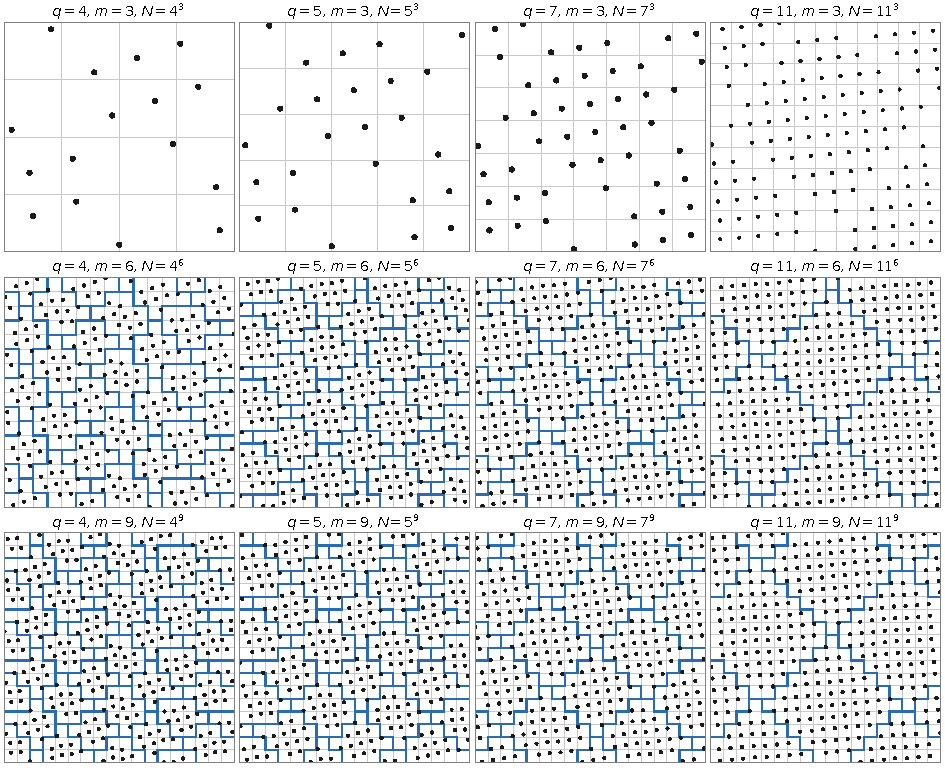
\includegraphics[width=\textwidth]{figs/fig_slab.pdf}
\caption{One slab of cells of $\mathcal P_{k,q}$ for $q=4,5,7,11$ and $m=3,6,9$: the points with $z$-cell $n_z=\lfloor q^k/2\rfloor$ and $(x,y)$-cells in a $W\times W$ window ($W=q$ for $m=3$, i.e. the whole slab; $W=16$ for $q=4$, $m=6$; $W=18$ otherwise; so $16$ to $324$ points), $xy$-projection in cell units (grey: cell boundaries). Blue: slip lines, i.e. cell edges across which the $(x,y)$ part of the step between the two points differs from that of $(I+M/q)e$ by more than half a cell (not drawn for $k=1$, where Proposition~\ref{prop:cell} does not apply). The patches of the tilted square lattice are a few cells wide for $q=4,5$ and grow with $q$.}
\label{fig:slab}
\end{figure}


\clearpage
\section{Formal verification}\label{app:formal}
\emph{Method.} The formalization uses Lean~4 \cite{dMU21}, toolchain \texttt{v4.35.0-rc3}, with the matching Mathlib \cite{Mathlib20}, and forms one Lake project with one statement library: $616$ theorem statements in twelve statement files, one for each part of the paper (Table~\ref{tab:lean}). The statement files contain no proofs; besides Mathlib they import only the definition modules of the project, which define the objects (nets from their generator matrices or graph forms, designs and searched data as explicit constants), so that statements and proofs use the same definitions. The proofs are in separate modules, and a solution file proves every statement under its name. Every proof is checked by the Lean kernel. The tool Comparator, with one configuration that lists the $616$ theorems, checks that the proved theorems are exactly those of the statement library and use only the permitted axioms, and re-checks the proofs with the Lean kernel and with a second, independent kernel (NanoDa).
Both kernels accept all $616$ theorems.
The only axioms used are \texttt{propext}, \texttt{Classical.choice} and \texttt{Quot.sound}; \texttt{native\_decide} is not used, and finite certificates are evaluated by \texttt{decide} in the kernel. Some proofs were reorganized for formalization (for instance, finite case splits replace the case analyses of Theorem~\ref{thm:sep} and Proposition~\ref{prop:twocoset}); the statements are those of the text.

\emph{Theorem~A as a self-contained entry.} Theorem~A also forms a separate entry in the format of the Palomar collection of formalizations: a statement file of $438$ lines that imports only Mathlib, copies verbatim the $43$ definitions that the statement reaches, and states Theorem~A together with three theorems that justify the data defined by choice: the columns of Definition~\ref{def:Ustar} are the only family with the properties required there, the positive generator $\gamma_j$ of Lemma~\ref{lem:sat} is unique, and the net of Definition~\ref{def:Ns} exists and does not depend on the choices made in its construction (the reduction modulo $q$ and the solution of the residual problem, Propositions~\ref{prop:Ns} and~\ref{prop:Gs}). Its solution derives the four theorems from the library, and Comparator checks the entry separately.

\emph{Blueprint.} A blueprint, made with \texttt{leanblueprint}, presents the results of the paper in its words, with their proofs, links every formalized result to the Lean declarations that prove it, and shows the dependency graph. The developments will be public at \url{https://github.com/lgruen/separated-nets-lean} and archived at Zenodo, DOI [to be added at deposit].

\emph{What is formalized.} Every theorem, proposition, lemma and corollary of the paper, every definition except Definition~\ref{def:geom} (which only introduces names), and the proved statements of the remarks listed in Table~\ref{tab:lean} are formalized, apart from the finite computations listed below.

\emph{Cited theorems.} Two formalized results use classical theorems that are not in our version of Mathlib; these theorems are not formalized here, and enter as explicit hypotheses. (1) The design $U_s$ (Remark~\ref{rem:Us}): the constant $1$ in $a_s\le e^{(1+o(1))s^2}$ is proved from the prime number theorem $\psi(x)\sim x$ \cite{Had96,dlVP96}; everything else is unconditional, including $(s-1)\psi(s-2)\le\log a_s\le(s-1)\psi(s-2)+s\log2$ for $s\ge6$ (a consequence of the bounds $L_s\le a_s\le L_s(s^2+2^{s-2})$ of Remark~\ref{rem:Us}, as $s^2+2^{s-2}\le2^s$ for $s\ge6$) and $\log a_s=\Theta(s^2)$ with explicit constants from Chebyshev's bounds. (2) Proposition~\ref{prop:cube}: parts (i)--(iii) with Haj\'os's theorem \cite{Haj42} and Keller's property for $s\le7$ \cite{Per40,BHMN20} as hypotheses; part (iv) unconditionally, except that its strict inequalities for $s=2,3$ use the optimal packing bounds (Thue's for $s=2$ \cite[Ch.~1]{CS99}, Hales's for $s=3$ \cite{Hal05}) as hypotheses. Some statements of the text are consequences of cited theorems that are neither formalized nor used as hypotheses: Niederreiter's discrepancy bound \cite{Nie87} (Remark~\ref{rem:lowdisc}); the optimality of the range of $q$ \cite[Cor.~2]{LNS96} (after Theorem~A and Lemma~\ref{lem:Ts}); the bound $s\le3$ in base two \cite[Cor.~5.11]{Nie87} (Remark~\ref{rem:base2}); the growth $\operatorname{lcm}(1,\dots,s-3)=e^{(1+o(1))s}$ after Proposition~\ref{prop:E} (the prime number theorem); and $K(F)\ge s^{1-O(1/\log\log s)}$ (in particular $K(F)\ge s^{1-o(1)}$) after Theorem~\ref{thm:Lstar}, a consequence of Wigert's divisor bound \cite[Thm.~317]{HW08}, whereas the $\operatorname{div}^*$ inequality of Theorem~\ref{thm:Lstar} itself is formalized.

\emph{Checked by scripts, not in Lean.} By decision, finite computations whose printed values no formalized result needs are checked by the scripts of Appendix~\ref{app:verify}, and, where Section~\ref{sec:formal} says so, by a second implementation, not in Lean:
\begin{itemize}
\item Theorem~\ref{thm:base23}(1), both at the resolutions below the certificate resolution $L$ (the exact minimum distances of the explicitly shifted nets) and beyond it (the certificate $v^*_L$ of the shifted net, which the formal statement of (1) beyond $L$ takes as a hypothesis), and the entries $.4699$ and $.2586$ of column (2) of Table~\ref{tab:base23}. Lean proves parts (2) and (3) for every $m\ge1$, with their constants, the nets of the theorem (seeds, chains and $t=0$ at every resolution) and the certificates $v^\circ_L$, checked in the kernel, and the lift theory (Definition~\ref{def:lift}, Lemmas~\ref{lem:lift}, \ref{lem:liftsep} and~\ref{lem:shiftcert}) in general;
\item the values $a^*_4,\dots,a^*_{10}$ of Table~\ref{tab:astar} and the base thresholds derived from them after Theorem~A, and the running time of the algorithm of Definition~\ref{def:Ustar};
\item the thresholds and scans of Tables~\ref{tab:Kdesigns} and~\ref{tab:practical}, including the bound $\delta N^{1/s}\ge0.8$ of Proposition~\ref{prop:k1designs}(2) and the thresholds stated after Proposition~\ref{prop:4D2}; the deficits, finite maxima and $t=0$ completions that Propositions~\ref{prop:4D2} and~\ref{prop:k1designs} state are formalized;
\item the values labelled \emph{computed} (Section~\ref{sec:formal}), among them the lines and spectral values of Remark~\ref{rem:projlines}, the resolutions at which $v^\circ_L$ vanishes (Remark~\ref{rem:shiftparity}), the comparison of $\mathcal W^*_p$ with $\mathcal W_p$ (Remark~\ref{rem:wstar}) and the shifts of Remark~\ref{rem:wshift} that break the lock.
\end{itemize}

\emph{Conventions fixed in the formal statements.} Where the text states a value up to sign, some formal statements fix the sign. For Lemma~\ref{lem:Tsplit} the sign is $+1$ for $V$ in the monomial basis, with the rows taken coordinate by coordinate and the points ordered $v_0,u_0,v_1,u_1,\dots$, $P$ before $Q$; this exact value is formally verified.

\begin{table}[tbp]\centering\footnotesize
\begin{tabular}{@{}>{\raggedright\arraybackslash}p{2.0cm}>{\raggedright\arraybackslash}p{8.1cm}>{\raggedright\arraybackslash}p{4.5cm}@{}}
\toprule
part of the paper & results & statement file; proof modules\\
\midrule
Sec.~\ref{sec:prelim} & Lems.~\ref{lem:nie}, \ref{lem:box}, \ref{lem:Ss}; Rem.~\ref{rem:K}; Def.~\ref{def:dshift} & \texttt{Prelim} (19); \texttt{F*}, \texttt{DShift}\\
Sec.~\ref{sec:frames} & Lems.~\ref{lem:hermite}, \ref{lem:Ts}, \ref{lem:Rs}, \ref{lem:CH}; Props.~\ref{prop:faure}, \ref{prop:Ns}, \ref{prop:Gs}, \ref{prop:F}; Def.~\ref{def:Ns}, Cor.~\ref{cor:tsk}; Rem.~\ref{rem:projlines} & \texttt{Frames} (50); \texttt{F*}, \texttt{Proj*}, \texttt{Obs*}\\
Sec.~\ref{sec:dims} & Thm.~A, Prop.~\ref{prop:D}, Lems.~\ref{lem:sat}, \ref{lem:adelic}, \ref{lem:babai}, Def.~\ref{def:Ustar}; the design $U_s$ of Rem.~\ref{rem:Us} (assuming PNT) & \texttt{ThmA} (66); \texttt{ThmA*}, \texttt{SU*}; Theorem~A also \texttt{Headline}\\
Sec.~\ref{sec:skel} & Lems.~\ref{lem:skelred}, \ref{lem:skelnec}, \ref{lem:skellat}, \ref{lem:G2N1}, \ref{lem:frameid}; Prop.~\ref{prop:skelcomp}, Cors.~\ref{cor:skelreach}, \ref{cor:frameid}; Defs.~\ref{def:S1}, \ref{def:G2rule}, \ref{def:S2}; Thms.~\ref{thm:S1}, \ref{thm:S2}; Prop.~\ref{prop:korobov4}; mathematical claims of Rem.~\ref{rem:codes} & \texttt{Skeleton} (67); \texttt{Sk*}, \texttt{S1*}, \texttt{S2*}, \texttt{T3*}\\
Sec.~\ref{sec:dim3} & Def.~\ref{def:net}, Thms.~\ref{thm:t0}, \ref{thm:main}, \ref{thm:sep}, Prop.~\ref{prop:cell}, Rem.~\ref{rem:lattice3}; Def.~\ref{def:col}, Thms.~\ref{thm:colmin}, \ref{thm:col}, Lem.~\ref{lem:shared}, Props.~\ref{prop:colfree}, \ref{prop:colshift}; Def.~\ref{def:B}, Prop.~\ref{prop:Bnet}, Thm.~\ref{thm:allm}, Rem.~\ref{rem:B2}; Cor.~\ref{cor:allm}, Rem.~\ref{rem:perprime} & \texttt{Dim3} (67; Def.~\ref{def:net} in \texttt{Frames}); \texttt{Main*}, \texttt{Net*}, \texttt{Sep*}, \texttt{Col*}, \texttt{D3*}, \texttt{KN*}\\
Sec.~\ref{sec:base23} & Def.~\ref{def:lift}, Lems.~\ref{lem:lift}, \ref{lem:liftsep}, \ref{lem:shiftcert}; Thm.~\ref{thm:base23}(2), (3), and (1) beyond $L$ given its certificate; Rem.~\ref{rem:shiftparity}; the proved statements of Rem.~\ref{rem:base2} & \texttt{Base23} (21); \texttt{B23*}\\
Sec.~\ref{sec:dgs} & Lem.~\ref{lem:shift}, Props.~\ref{prop:shift}, \ref{prop:linf}; Cors.~\ref{cor:allmshift}, \ref{cor:dgs}; Rems.~\ref{rem:shiftshared}, \ref{rem:dgsfinite} & \texttt{DGS} (64); \texttt{*Shift*}, \texttt{DGS*}\\
Secs.~\ref{sec:deficit}--\ref{sec:drift} & Def.~\ref{def:K}, Props.~\ref{prop:Dprime}, \ref{prop:ceil}, Lem.~\ref{lem:Kone}, Cors.~\ref{cor:ceil3}, \ref{cor:ceils}, Props.~\ref{prop:4D2}, \ref{prop:k1}, \ref{prop:k1designs}; Rem.~\ref{rem:pm1}; the proved statements of Rem.~\ref{rem:sign}; Prop.~\ref{prop:P2}, Def.~\ref{def:Ktrue}, Thms.~\ref{thm:L}, \ref{thm:O5}; Lems.~\ref{lem:O}, \ref{lem:C}, Prop.~\ref{prop:E}, Thm.~\ref{thm:Lstar}; Lem.~\ref{lem:drift}, Cor.~\ref{cor:colceil}, Thm.~\ref{thm:O} & \texttt{Deficit} (75); \texttt{Deficit*}, \texttt{Obs*}, \texttt{Ceil}, \texttt{D4D2*}, \texttt{K1*}, \texttt{Lstar*}, \texttt{Col*}\\
Sec.~\ref{sec:whylat} & Lems.~\ref{lem:hom}, \ref{lem:phase}, Cor.~\ref{cor:linoff}; Prop.~\ref{prop:cube} (assuming Haj\'os, Keller for $s\le7$, packing bounds) & \texttt{WhyLat} (14); \texttt{WL*}\\
Secs.~\ref{sec:S1E}--\ref{sec:wnet} & Prop.~\ref{prop:S1E}, Table~\ref{tab:S1E}; Prop.~\ref{prop:twocoset}; Props.~\ref{prop:wnet}, \ref{prop:wfamily}, Lem.~\ref{lem:wwrap}, Rems.~\ref{rem:wstar}, \ref{rem:wshift} & \texttt{Large} (81); \texttt{S1E*}, \texttt{SkCert*}; \texttt{QUNetsM3/TC*}, \texttt{QUNetsM3/W*}\\
Secs.~\ref{sec:Pnohalf}--\ref{sec:halfms} & Prop.~\ref{prop:P}; Def.~\ref{def:split}, Lems.~\ref{lem:Tsplit}, \ref{lem:Rsplit}, Prop.~\ref{prop:Gsplit} and the remark after it; Lem.~\ref{lem:Hs}, Prop.~\ref{prop:Hk}, Thm.~\ref{thm:HL}, Prop.~\ref{prop:HL5}; Lem.~\ref{lem:R2}, Prop.~\ref{prop:half5}, Rem.~\ref{rem:accounting}, Thm.~\ref{thm:D} & \texttt{Split} (78); \texttt{Split*}, \texttt{HL*}, \texttt{Half*}, \texttt{Q5*}, \texttt{TD*}, \texttt{Acct*}\\
App.~\ref{app:perprime} & Defs.~\ref{def:ppdesign}, \ref{def:pprelax}, Prop.~\ref{prop:ppsep}, Props.~\ref{prop:pp1}, \ref{prop:pp2}, Lem.~\ref{lem:ppinv}, Rem.~\ref{rem:ppshift}; Table~\ref{tab:perprime} & \texttt{Appendix} (14); \texttt{PP*}, \texttt{KN*}\\
\bottomrule
\end{tabular}
\medskip
\caption{Formal verification: for each part of the paper, the statement file of the Lean library that states its results (in \texttt{QUNets/Statements/}, with the number of its theorems; $616$ in all) and the principal proof modules (in \texttt{Z3Net/} unless stated; \texttt{*} stands for any part of a name). Several results are also used, or restated, in other files. ``Assuming~$X$'' means that the result uses the classical theorems~$X$, which are not in Mathlib, as explicit hypotheses (PNT, the prime number theorem; Appendix~\ref{app:formal}). \texttt{Headline} is the self-contained entry for Theorem~A.}
\label{tab:lean}
\end{table}

\section{Computations}\label{app:verify}
The computed values printed in the paper, none of which is used in a proof, the finite certificates of Theorem~\ref{thm:base23}, Theorem~\ref{thm:D} and Propositions~\ref{prop:korobov4} and~\ref{prop:half5}, and the figures are reproduced by the programs in the folder \texttt{scripts/} of the accompanying software deposit (Python~3, run with \texttt{uv}, and C++). A driver script builds and runs all of them in a few minutes on one laptop (the certificates of Theorem~\ref{thm:base23} use several cores if available); it fails if a value differs from the one printed here or a regenerated figure differs from the published one. The README of the folder lists, for each program, what it reproduces:
\begin{itemize}
\item the base-$2$ $(0,m,3)$-net of \cite[Sec.~2]{GK09}, built from its generator matrices and, independently, by a re-implementation of the C routine printed in \cite{GK09}, with the $(0,m,3)$ property by box counting and the exact toroidal minimum distance: $\delta N^{1/3}=.750$, $.649$, $.486$, $.433$, $.472$, $.466$, $.424$, $.447$, $.375$, $.265$, $.186$ for $m=3,\dots,13$ (Section~\ref{sec:intro});
\item the two-dimensional nets of Remark~\ref{rem:gk2d} for $m=4,6,8,10$: the $(0,m,2)$ property; for (iii), all slides along their lines that keep $t=0$ and their distances from lattice slides ($m=4,6,8$), and, for even $8\le m\le20$, the $(0,m,2)$ property and the exact minimum distances, in the tiling metric, of the re-scrambled nets and of the nets themselves;
\item the enumeration of one-per-cube lattices in $\frac1e\Z^3$, $e\le11$, and the affinity check of Remark~\ref{rem:cubecost};
\item the exact minimum distances of Table~\ref{tab:c}, by a toroidal neighbour-cell scan of nets rebuilt from Definition~\ref{def:net}, with the other values of this table;
\item the computed values after Proposition~\ref{prop:twocoset} (Figure~\ref{fig:arctwocoset}(c));
\item the evaluations of proved formulas in Table~\ref{tab:skel};
\item Table~\ref{tab:astar} ($a^*_s$ and the largest entries computed from Definition~\ref{def:Ustar}, $5a^*_s+4$, the bound of Theorem~A, $a_s$ of $U_s$) and the values derived from it in the Introduction and in Table~\ref{tab:Kdesigns};
\item the certified deficits, $\sigma_{\max}(F)$, $q_{\mathrm{tail}}$ and thresholds of Table~\ref{tab:Kdesigns} ($K$ and thresholds for $s\le6$; $\sigma_{\max}$ and $q_{\mathrm{tail}}$ for $s\le8$) and the finite parts of Proposition~\ref{prop:4D2}, by the exact relaxation of Lemma~\ref{lem:Ss} on the designs of Appendix~\ref{app:designs}; and the $K_1$, thresholds and sizes of Table~\ref{tab:practical} (the per-prime $t=0$ completions of Proposition~\ref{prop:k1designs} are not rerun by these scripts; they were reproduced by independent implementations and are checked in the Lean kernel, Section~\ref{sec:formal});
\item the certificates of Theorem~\ref{thm:base23} (Table~\ref{tab:base23}): the chains replayed from the seeds, $t=0$ at every resolution, the integers $v^*_L$ of Lemma~\ref{lem:liftsep} with the proviso $g_L\le b^{L/3}-Wb^{-2L/3}$, the exact minima between the seed and the certificate resolutions, and the small-$m$ nets, by the checker of the deposit (with OpenMP about half a minute on ten cores); for part~(3), the integers $v^\circ_L$, the exact minima over all digital shifts at the resolutions up to $L$ and of the small-$m$ nets (Lemma~\ref{lem:shiftcert}), and the freezing of the chains, by a second checker (a few seconds);
\item the column nets of Section~\ref{sec:m3}: Theorem~\ref{thm:colmin} on random column point sets against an exact brute-force distance, the closed forms of Theorem~\ref{thm:col} against two exact kernels at every $q\le241$ coprime to $6$ (composites included), the box minors, all digital shifts at small $q$ against Proposition~\ref{prop:colshift}, the class maximum of the digital column nets against Theorem~\ref{thm:O}, the comparison with $\mathcal T_p$ after Proposition~\ref{prop:twocoset}, and the comparison nets with a common second digit of Figure~\ref{fig:drift}(c);
\item the rank-one nets of Section~\ref{sec:wnet}, Proposition~\ref{prop:wnet}: the box minors of $\mathcal W_p$, Lemma~\ref{lem:wwrap} by enumeration of all cells at small $p$, the numerical steps of the proof of Proposition~\ref{prop:wnet} in exact arithmetic (the rules of part~(2) against the lemma, Table~\ref{tab:wcontacts} and the tangent-line constants, and, independently, the full quadratic of every option in each of the $24$ classes of $p$ modulo $48$), the relaxation at every prime $53\le p\le3000$, the pair of part~(3), the exact minimum distances of $\mathcal W_p$ at every prime $5\le p\le199$ and at $307$, $353$ (the finite part of (4)), the comparison with $\mathcal T_p$, the layer with a geometric digit shared by two coordinates at $p=307$ and its value in the limit model, and the digital shifts of Remark~\ref{rem:wshift};
\item for Proposition~\ref{prop:wfamily} and Remark~\ref{rem:wstar}: the constants and every numerical fact of the proof in exact arithmetic, the value $F(\psi^*)=\mu^{*2}$ from all options, the identity $F_p(u)=F(u/p)$ and $\max_uF_p(u)<\mu^{*2}$ over all $u$ at small primes, the box minors and the bound with $K$ for $\mathcal W^*_p$, the thresholds, and the exact minimum distances of $\mathcal W_p$ and $\mathcal W^*_p$ at the primes $p\le1009$ where they differ (recomputed by the scripts at $193$, $241$, $337$; at the other five primes the values come from two separate distance programs that agree, and are not rerun by the driver);
\item the certificates of Proposition~\ref{prop:half5} (the $126$ box minors, the exact scans of Lemma~\ref{lem:R2} and of Proposition~\ref{prop:Hk}(1) with their monotone tails, the finite check of the limit), the constants of Remark~\ref{rem:accounting} and Remark~\ref{rem:M5}, the exact minimum distances of $\mathcal Q^*_p$ for $7\le p\le61$, and the enumerations of Theorem~\ref{thm:D} and of the text after it;
\item the data printed in Proposition~\ref{prop:korobov4}, Remark~\ref{rem:cubecost} and Tables~\ref{tab:ppdesigns}, \ref{tab:S1Ekappa}, \ref{tab:b23seeds}, compared with their sources entry by entry, with the finite checks in the proof of Proposition~\ref{prop:korobov4}, the layer of Remark~\ref{rem:accounting} and the identity and estimates in the proof of Proposition~\ref{prop:twocoset};
\item every printed decimal bound, recomputed in exact arithmetic and checked to be truncated or rounded as stated in Section~\ref{sec:conv} (this check also reads the integers $T_p$ of Table~\ref{tab:perprime} from the formalization);
\item the figures, including those of Part~I (Figures~\ref{fig:thmA}, \ref{fig:base23}, \ref{fig:projlines}, \ref{fig:col}) and of the accounting (Figures~\ref{fig:drift}, \ref{fig:half5}, \ref{fig:wnet}), each regenerated by its script, which also asserts the properties stated in its caption.
\end{itemize}

\begin{thebibliography}{99}
\bibitem{BHMN20} J.~Brakensiek, M.~Heule, J.~Mackey, D.~Narv\'aez, \emph{The resolution of Keller's conjecture}, J. Automat. Reason. 66 (2022) 277--300, doi:10.1007/s10817-022-09623-5; conference version in: IJCAR 2020, Lecture Notes in Comput. Sci. 12166, Springer, 2020, 48--65, doi:10.1007/978-3-030-51074-9\_4; arXiv:1910.03740.
\bibitem{BS83} E.~S.~Barnes, N.~J.~A.~Sloane, \emph{New lattice packings of spheres}, Canad. J. Math. 35 (1983) 117--130, doi:10.4153/cjm-1983-008-1.
\bibitem{CE03} H.~Cohn, N.~Elkies, \emph{New upper bounds on sphere packings I}, Ann. of Math. 157 (2003) 689--714, doi:10.4007/annals.2003.157.689; arXiv:math/0110009.
\bibitem{CKMRV17} H.~Cohn, A.~Kumar, S.~D.~Miller, D.~Radchenko, M.~Viazovska, \emph{The sphere packing problem in dimension $24$}, Ann. of Math. 185 (2017) 1017--1033, doi:10.4007/annals.2017.185.3.8; arXiv:1603.06518.
\bibitem{CM67} R.~R.~Coveyou, R.~D.~MacPherson, \emph{Fourier analysis of uniform random number generators}, J. ACM 14 (1967) 100--119, doi:10.1145/321371.321379.
\bibitem{Coo86} R.~L.~Cook, \emph{Stochastic sampling in computer graphics}, ACM Trans. Graph. 5 (1986) 51--72, doi:10.1145/7529.8927.
\bibitem{COU01} L.~Clozel, H.~Oh, E.~Ullmo, \emph{Hecke operators and equidistribution of Hecke points}, Invent. Math. 144 (2001) 327--351, doi:10.1007/s002220100126.
\bibitem{CP76} R.~Cranley, T.~N.~L.~Patterson, \emph{Randomization of number theoretic methods for multiple integration}, SIAM J. Numer. Anal. 13 (1976) 904--914, doi:10.1137/0713071.
\bibitem{CS99} J.~H.~Conway, N.~J.~A.~Sloane, \emph{Sphere Packings, Lattices and Groups}, 3rd ed., Springer, 1999.
\bibitem{DGLPS1} J.~Dick, T.~Goda, G.~Larcher, F.~Pillichshammer, K.~Suzuki, \emph{On the quasi-uniformity properties of quasi-Monte Carlo point sets and sequences, Part I: lattices and Kronecker sequences}, Math. Comp. (2026), doi:10.1090/mcom/4264; arXiv:2502.06202 (theorem numbers cited from arXiv v2).
\bibitem{DGS2} J.~Dick, T.~Goda, K.~Suzuki, \emph{On the quasi-uniformity properties of quasi-Monte Carlo point sets and sequences, Part II: digital nets and sequences}, Math. Comp. (2026), doi:10.1090/mcom/4263; arXiv:2501.18226 (theorem numbers cited from arXiv v2).
\bibitem{dlVP96} C.-J.~de la Vall\'ee Poussin, \emph{Recherches analytiques sur la th\'eorie des nombres premiers}, Ann. Soc. Sci. Bruxelles 20 B (1896) 183--256.
\bibitem{dMU21} L.~de Moura, S.~Ullrich, \emph{The Lean~4 theorem prover and programming language}, in: Automated Deduction -- CADE 28, Lecture Notes in Comput. Sci. 12699, Springer, 2021, 625--635, doi:10.1007/978-3-030-79876-5\_37.
\bibitem{DP10} J.~Dick, F.~Pillichshammer, \emph{Digital Nets and Sequences: Discrepancy Theory and Quasi-Monte Carlo Integration}, Cambridge Univ. Press, 2010.
\bibitem{EO06} A.~Eskin, H.~Oh, \emph{Ergodic theoretic proof of equidistribution of Hecke points}, Ergodic Theory Dynam. Systems 26 (2006) 163--167, doi:10.1017/s0143385705000428; arXiv:math/0409507.
\bibitem{Fau82} H.~Faure, \emph{Discr\'epance de suites associ\'ees \`a un syst\`eme de num\'eration (en dimension $s$)}, Acta Arith. 41 (1982) 337--351, doi:10.4064/aa-41-4-337-351.
\bibitem{FL09} H.~Faure, C.~Lemieux, \emph{Generalized Halton sequences in 2008: a comparative study}, ACM Trans. Model. Comput. Simul. 19 (2009), Art.~15, 1--31, doi:10.1145/1596519.1596520.
\bibitem{GHS26} T.~Goda, R.~Hofer, K.~Suzuki, \emph{Disproving the quasi-uniformity of the Halton sequences and of some Halton-type sequences}, J. Complexity 95 (2026) 102047, doi:10.1016/j.jco.2026.102047; arXiv:2511.21153 (theorem numbers cited from arXiv v2).
\bibitem{GHSK08} L.~Gr\"unschlo{\ss}, J.~Hanika, R.~Schwede, A.~Keller, \emph{$(t,m,s)$-nets and maximized minimum distance}, in: A.~Keller, S.~Heinrich, H.~Niederreiter (eds.), Monte Carlo and Quasi-Monte Carlo Methods 2006, Springer, 2008, 397--412, doi:10.1007/978-3-540-74496-2\_23.
\bibitem{GK09} L.~Gr\"unschlo{\ss}, A.~Keller, \emph{$(t,m,s)$-nets and maximized minimum distance, Part II}, in: P.~L'Ecuyer, A.~B.~Owen (eds.), Monte Carlo and Quasi-Monte Carlo Methods 2008, Springer, 2009, 395--409, doi:10.1007/978-3-642-04107-5\_25.
\bibitem{Had96} J.~Hadamard, \emph{Sur la distribution des z\'eros de la fonction $\zeta(s)$ et ses cons\'equences arithm\'etiques}, Bull. Soc. Math. France 24 (1896) 199--220, doi:10.24033/bsmf.545.
\bibitem{Haj42} G.~Haj\'os, \emph{\"Uber einfache und mehrfache Bedeckung des $n$-dimensionalen Raumes mit einem W\"urfelgitter}, Math. Z. 47 (1942) 427--467, doi:10.1007/bf01180974.
\bibitem{Hal05} T.~C.~Hales, \emph{A proof of the Kepler conjecture}, Ann. of Math. 162 (2005) 1065--1185, doi:10.4007/annals.2005.162.1065.
\bibitem{Ham60} J.~M.~Hammersley, \emph{Monte Carlo methods for solving multivariable problems}, Ann. New York Acad. Sci. 86 (1960) 844--874, doi:10.1111/j.1749-6632.1960.tb42846.x.
\bibitem{HW08} G.~H.~Hardy, E.~M.~Wright, \emph{An Introduction to the Theory of Numbers}, 6th ed., revised by D.~R.~Heath-Brown and J.~H.~Silverman, Oxford Univ. Press, 2008.
\bibitem{He17} X.~He, \emph{Rotated sphere packing designs}, J. Amer. Statist. Assoc. 112 (2017) 1612--1622, doi:10.1080/01621459.2016.1222289.
\bibitem{He19} X.~He, \emph{Interleaved lattice-based maximin distance designs}, Biometrika 106 (2019) 453--464, doi:10.1093/biomet/asy069; arXiv:1807.02289.
\bibitem{He21} X.~He, \emph{Lattice-based designs with quasi-optimal separation distance on all projections}, Biometrika 108 (2021) 443--454, doi:10.1093/biomet/asaa057; arXiv:1709.02062.
\bibitem{HP55} M.~Hall, L.~J.~Paige, \emph{Complete mappings of finite groups}, Pacific J. Math. 5 (1955) 541--549, doi:10.2140/pjm.1955.5.541.
\bibitem{HS19} R.~Hofer, K.~Suzuki, \emph{A complete classification of digital $(0,m,3)$-nets and digital $(0,2)$-sequences in base $2$}, Unif. Distrib. Theory 14 (2019) 43--52, doi:10.2478/udt-2019-0004; arXiv:1807.04383.
\bibitem{KB79} R.~Kannan, A.~Bachem, \emph{Polynomial algorithms for computing the Smith and Hermite normal forms of an integer matrix}, SIAM J. Comput. 8 (1979) 499--507, doi:10.1137/0208040.
\bibitem{Knu97} D.~E.~Knuth, \emph{The Art of Computer Programming, Vol.~2: Seminumerical Algorithms}, 3rd ed., Addison-Wesley, 1997.
\bibitem{KO14} W.~Kositwattanarerk, F.~Oggier, \emph{Connections between Construction D and related constructions of lattices}, Des. Codes Cryptogr. 73 (2014) 441--455, doi:10.1007/s10623-014-9939-3; arXiv:1308.6175.
\bibitem{Kor59} N.~M.~Korobov, \emph{The approximate computation of multiple integrals}, Dokl. Akad. Nauk SSSR 124 (1959) 1207--1210.
\bibitem{Kri21} R.~Kritzinger, \emph{Dispersion of digital $(0,m,2)$-nets}, Monatsh. Math. 195 (2021) 155--171, doi:10.1007/s00605-021-01525-9; arXiv:2004.14760.
\bibitem{Len77} H.~W.~Lenstra, Jr., \emph{Euclidean number fields of large degree}, Invent. Math. 38 (1976/77) 237--254, doi:10.1007/bf01403131.
\bibitem{L15} C.~Lemieux, \emph{Tractability using periodized generalized Faure sequences}, J. Complexity 31 (2015) 42--56, doi:10.1016/j.jco.2014.08.001.
\bibitem{LF09} C.~Lemieux, H.~Faure, \emph{New perspectives on $(0,s)$-sequences}, in: P.~L'Ecuyer, A.~B.~Owen (eds.), Monte Carlo and Quasi-Monte Carlo Methods 2008, Springer, 2009, 113--130, doi:10.1007/978-3-642-04107-5\_7.
\bibitem{LNS96} G.~Larcher, H.~Niederreiter, W.~Ch.~Schmid, \emph{Digital nets and sequences constructed over finite rings and their application to quasi-Monte Carlo integration}, Monatsh. Math. 121 (1996) 231--253, doi:10.1007/bf01298952.
\bibitem{LP01} G.~Larcher, F.~Pillichshammer, \emph{Walsh series analysis of the $L_2$-discrepancy of symmetrisized point sets}, Monatsh. Math. 132 (2001) 1--18, doi:10.1007/s006050170054.
\bibitem{LS92} J.~C.~Lagarias, P.~W.~Shor, \emph{Keller's cube-tiling conjecture is false in high dimensions}, Bull. Amer. Math. Soc. (N.S.) 27 (1992) 279--283, doi:10.1090/s0273-0979-1992-00318-x; arXiv:math/9210222.
\bibitem{Mac02} J.~Mackey, \emph{A cube tiling of dimension eight with no facesharing}, Discrete Comput. Geom. 28 (2002) 275--279, doi:10.1007/s00454-002-2801-9.
\bibitem{Mat98} J.~Matou\v sek, \emph{On the $L_2$-discrepancy for anchored boxes}, J. Complexity 14 (1998) 527--556, doi:10.1006/jcom.1998.0489.
\bibitem{Mathlib20} The mathlib Community, \emph{The Lean mathematical library}, in: Proc. 9th ACM SIGPLAN Int. Conf. on Certified Programs and Proofs (CPP 2020), ACM, 2020, 367--381, doi:10.1145/3372885.3373824.
\bibitem{MS77} F.~J.~MacWilliams, N.~J.~A.~Sloane, \emph{The Theory of Error-Correcting Codes}, North-Holland, 1977.
\bibitem{Nie87} H.~Niederreiter, \emph{Point sets and sequences with small discrepancy}, Monatsh. Math. 104 (1987) 273--337, doi:10.1007/bf01294651.
\bibitem{Owe95} A.~B.~Owen, \emph{Randomly permuted $(t,m,s)$-nets and $(t,s)$-sequences}, in: H.~Niederreiter, P.~J.-S.~Shiue (eds.), Monte Carlo and Quasi-Monte Carlo Methods in Scientific Computing, Lecture Notes in Statist. 106, Springer, 1995, 299--317, doi:10.1007/978-1-4612-2552-2\_19.
\bibitem{Pai51} L.~J.~Paige, \emph{Complete mappings of finite groups}, Pacific J. Math. 1 (1951) 111--116, doi:10.2140/pjm.1951.1.111.
\bibitem{Per40} O.~Perron, \emph{\"Uber l\"uckenlose Ausf\"ullung des $n$-dimensionalen Raumes durch kongruente W\"urfel}, Math. Z. 46 (1940) 1--26, doi:10.1007/bf01181421; \emph{II}, Math. Z. 46 (1940) 161--180, doi:10.1007/bf01181436.
\bibitem{PFA09} L.~Panek, M.~Firer, M.~M.~S.~Alves, \emph{Symmetry groups of Rosenbloom--Tsfasman spaces}, Discrete Math. 309 (2009) 763--771, doi:10.1016/j.disc.2008.01.013.
\bibitem{RS85} R.~M.~Roth, G.~Seroussi, \emph{On generator matrices of MDS codes (Corresp.)}, IEEE Trans. Inform. Theory 31 (1985) 826--830, doi:10.1109/tit.1985.1057113.
\bibitem{RT97} M.~Yu.~Rosenbloom, M.~A.~Tsfasman, \emph{Codes for the $m$-metric}, Probl. Inf. Transm. 33 (1997) 45--52.
\bibitem{Rud26} L.~Rudolph, \emph{The even-order Gr\"unschlo{\ss}--Keller permutation nets are $(0,m,2)$-nets}, preprint, Zenodo, version 1.0.0, 2026, doi:10.5281/zenodo.22264675.
\bibitem{SG26} N.~Sakai, T.~Goda, \emph{Space-filling lattice designs for computer experiments}, arXiv:2602.15390 (2026).
\bibitem{SJ94} I.~H.~Sloan, S.~Joe, \emph{Lattice Methods for Multiple Integration}, Oxford Univ. Press, 1994.
\bibitem{Skr01} M.~M.~Skriganov, \emph{Coding theory and uniform distributions}, Algebra i Analiz 13 (2001) 191--239; English transl. St. Petersburg Math. J. 13 (2002) 301--337; arXiv:math/9909163 (theorem numbers cited from the arXiv version).
\bibitem{Sob67} I.~M.~Sobol', \emph{On the distribution of points in a cube and the approximate evaluation of integrals}, Zh. Vychisl. Mat. Mat. Fiz. 7 (1967) 784--802; English transl. USSR Comput. Math. Math. Phys. 7 (1967) 86--112, doi:10.1016/0041-5553(67)90144-9.
\bibitem{SS07} I.~M.~Sobol', B.~V.~Shukhman, \emph{Quasi-random points keep their distance}, Math. Comput. Simulation 75 (2007) 80--86, doi:10.1016/j.matcom.2006.09.004.
\bibitem{Suz25} K.~Suzuki, \emph{Exact $\ell^\infty$-separation radius of Sobol' sequences in dimension~$2$}, arXiv:2508.14803 (2025).
\bibitem{Suz26} K.~Suzuki, \emph{Separation properties of scrambled digital nets and related random point sets}, arXiv:2607.29063 (2026).
\bibitem{Tez93} S.~Tezuka, \emph{Polynomial arithmetic analogue of Halton sequences}, ACM Trans. Model. Comput. Simul. 3 (1993) 99--107, doi:10.1145/169702.169694.
\bibitem{Tez95} S.~Tezuka, \emph{Uniform Random Numbers: Theory and Practice}, Kluwer, 1995.
\bibitem{TV06} R.~Tavildar, P.~Viswanath, \emph{Approximately universal codes over slow-fading channels}, IEEE Trans. Inform. Theory 52 (2006) 3233--3258, doi:10.1109/tit.2006.876226; arXiv:cs/0512017.
\bibitem{vDHHM07} E.~R.~van Dam, B.~Husslage, D.~den Hertog, H.~Melissen, \emph{Maximin Latin hypercube designs in two dimensions}, Oper. Res. 55 (2007) 158--169, doi:10.1287/opre.1060.0317.
\bibitem{vDRH09} E.~R.~van Dam, G.~Rennen, B.~Husslage, \emph{Bounds for maximin Latin hypercube designs}, Oper. Res. 57 (2009) 595--608, doi:10.1287/opre.1080.0604.
\bibitem{VG06} P.~O.~Vontobel, A.~Ganesan, \emph{On universally decodable matrices for space-time coding}, Des. Codes Cryptogr. 41 (2006) 325--342, doi:10.1007/s10623-006-9019-4; arXiv:cs/0601075.
\bibitem{Via17} M.~S.~Viazovska, \emph{The sphere packing problem in dimension $8$}, Ann. of Math. 185 (2017) 991--1015, doi:10.4007/annals.2017.185.3.7.
\end{thebibliography}

\end{document}

